\documentclass{book}
\usepackage{a4wide}

%% possible fonts -- in order of preference
%%\usepackage{palatino}
\usepackage{bookman}
%%\usepackage{charter}
%%\usepackage{newcent}
%%\usepackage{times}
%%\usepackage{avant}
%%\usepackage{helvet}
%%\usepackage{sans}
%%\usepackage{chancery}

\usepackage[svgnames]{xcolor}	% for color text support
\usepackage[T1]{fontenc}
\usepackage[11pt]{moresize}
\usepackage{setspace}
\usepackage{ifpdf}
\usepackage{verbatim}   % for the comment environment
\usepackage{makeidx}
\usepackage{longtable}  %% page wrapping table environment
\usepackage{colortbl}   %% colors for tables
\usepackage{fancyvrb}   %% the "Verbatim" environment
\usepackage{fancyhdr}   %% custom headers and footers
\usepackage{multicol}
\usepackage{enumitem}   %% compact bullet lists with \begin{itemize}[noitemsep]
\usepackage{csquotes}   %% for the "displayquote" environment
\usepackage{upquote}
\usepackage{listings}   %% source code listings with syntax highlight (lstxxx commands)
\usepackage[tight]{shorttoc}   %% for generating a second table of contents, only containing chapter titles

\usepackage{tocbibind}  %% makes Bibliography and Index show up in TOC
\settocbibname{References}

\setlength{\textwidth}{160mm}
%\setlength{\oddsidemargin}{12.5mm}
%\setlength{\evensidemargin}{12.5mm}
%\setlength{\topmargin}{0mm}
\setlength{\textheight}{220mm}
%\setlength{\parskip}{1ex}
%\setlength{\parindent}{5ex}

\hfuzz=10pt %% suppress less severe 'overfull hbox' warnings

\renewcommand{\bottomfraction}{0.9}
\renewcommand{\topfraction}{0.9}
\renewcommand{\floatpagefraction}{0.9}

\newenvironment{htmlonly}{\expandafter\comment}{\expandafter\endcomment}
\newcommand{\pdfonly}{}

%% try to cure overfull hboxes
%% \tolerance=500

%% for navigation in dvi files, only needed by old teTeX versions
%%\usepackage{srcltx}

%% try this for spell checking: cat ess2002.tex | ispell -l -t -a | sort | uniq | more

%%
%% OMNeT++ logo, use as {\opp}
%%
\makeatletter
%%\DeclareRobustCommand{\omnetpp}{OM\-NeT\kern-.18em++\@}
\DeclareRobustCommand{\omnetpp}{OMNeT++\@}
\makeatother

\newcommand{\omnest}{OMNEST}
\newcommand{\oppversion}{5.x}

%%
%% *** CHECK SETTING BELOW BEFORE RELEASES ***
%%
\newif\ifcommercial
%\commercialtrue

\ifcommercial
  \newcommand{\opp}{\omnest}
\else
  \newcommand{\opp}{\omnetpp}
\fi

%%
%% PDF Header
%%
% note: \ifpdf now comes from the ifpdf package
%\newif\ifpdf
%\ifx\pdfoutput\undefined
%  \pdffalse
%\else
%  \pdfoutput=1
%  \pdftrue
%\fi
%% PDF-Info
\ifpdf
  \usepackage[pdftex]{graphicx}
  \usepackage[plainpages=false,linktocpage,bookmarksnumbered=true,pdftex]{hyperref}   %% automatic hyperlinking
  \pdfcompresslevel=9
  \pdfinfo{/Author (Andras Varga)
    /Title (Simulation Manual)
    /Subject ()
    /Keywords (OMNeT++ simulation manual)}
\else
  \usepackage{graphicx}
  \usepackage[plainpages=false]{hyperref}   %% automatic hyperlinking
\fi

%%
%% Generate Index
%%
\makeindex


%%
%% Link colors (hyperref package)
%%
\definecolor{MyDarkBlue}{rgb}{0.16,0.16,0.5}
%% XXX the next line apparently screws up all links except in TOC! they'll be colored nicely, but won't work.
%\hypersetup{
%    colorlinks=true,
%    linkcolor=MyDarkBlue,
%    anchorcolor=MyDarkBlue,
%    citecolor=MyDarkBlue,
%    filecolor=MyDarkBlue,
%    menucolor=MyDarkBlue,
%    runcolor=MyDarkBlue,
%    urlcolor=blue,
%}

%%
%% Heading and Footer
%%
\pagestyle{fancy}
\fancyhf{}
\renewcommand{\footrulewidth}{0.5pt}
\renewcommand{\chaptermark}[1]{\markboth{#1}{}}
\lhead{{\opp} Simulation Manual -- \leftmark}
\rfoot{\thepage}

%% this is used for chapter start pages
\fancypagestyle{plain}{
    \rfoot{\thepage}
}

%%
%% Use \begin{graybox}...\end{graybox} for notes
%%
\definecolor{MyGray}{rgb}{0.85,0.85,1.0}
\makeatletter\newenvironment{graybox}%
   {\begin{flushright}\begin{lrbox}{\@tempboxa}\begin{minipage}[r]{0.95\textwidth}}%
   {\end{minipage}\end{lrbox}\colorbox{MyGray}{\usebox{\@tempboxa}}\end{flushright}}%
\makeatother


\newenvironment{note}{\begin{graybox}\textbf{NOTE: }}{\end{graybox}}
\newenvironment{hint}{\begin{graybox}\textbf{HINT: }}{\end{graybox}}
\newenvironment{warning}{\begin{graybox}\textbf{WARNING: }}{\end{graybox}}
\newenvironment{caution}{\begin{graybox}\textbf{CAUTION: }}{\end{graybox}}
\newenvironment{rationale}{\begin{graybox}\textbf{Rationale: }}{\end{graybox}}
\newenvironment{important}{\begin{graybox}\textbf{IMPORTANT: }}{\end{graybox}}

%%
%% Set up listings package
%%
\lstloadlanguages{C++,Python,make,perl,tcl,XML,R,Matlab}

%% See listings.pdf,pp20
\lstdefinelanguage{NED} {
    morekeywords={allowunconnected,bool,channel,channelinterface,connections,const,
                  default,double,exists,extends,false,for,gates,if,import,index,inf,inout,input,
                  int,like,module,moduleinterface,nan,network,output,package,parameters,
                  property,simple,sizeof,string,submodules,this,true,typename,types,
                  volatile,xml,xmldoc},
    sensitive=true,
    morecomment=[l]{//},
    morestring=[b]",
}
\lstdefinelanguage{MSG} {
    morekeywords={abstract,bool,char,class,cplusplus,double,enum,extends,false,
                  fields,int,long,message,namespace,noncobject,packet,properties,
                  readonly,short,string,struct,true,unsigned},
    sensitive=true,
    morecomment=[l]{//},
    morestring=[b]",
}
\lstdefinelanguage{inifile} {
    morekeywords={},
    sensitive=true,
    morecomment=[l]{\#},
    morestring=[b]",
}
\lstdefinelanguage{pseudocode} {
    morekeywords={if,then,else,otherwise,whenever,while},
    sensitive=true,
    morecomment=[l]{//},
    morestring=[b]",
    mathescape=true,
}

%% thick ruler on the left; also, designate backtick as LaTeX escape character
%% (e.g. \opp needs to be written as `\opp` inside listing blocks)
\lstset{
    escapechar=`,
    basicstyle=\ttfamily,
    identifierstyle=\color{Black},
    stringstyle=\color{DarkBlue},
    commentstyle=\color{SeaGreen},
    keywordstyle=\bfseries\color{Purple},
    showstringspaces=false,
    frame=leftline,
    framesep=10pt,
    framerule=3pt,
    xleftmargin=15pt
}

\definecolor{NEDRulerColor}{rgb}{0.8,1.0,0.8}  % pale green
\definecolor{MSGRulerColor}{rgb}{0.8,1.0,0.8}  % pale green
\definecolor{CPPRulerColor}{rgb}{0.8,0.8,1.0}  % pale blue
\definecolor{PythonRulerColor}{rgb}{0.8,0.8,1.0}  % pale blue
\definecolor{IniRulerColor}{rgb}{0.9,0.9,0.2}  % pale yellow
\definecolor{FileListingRulerColor}{rgb}{0.85,0.85,0.85}  % grey
%\definecolor{CommandLineRulerColor}{rgb}{0.9,0.9,0.2}
\definecolor{PseudoCodeRulerColor}{rgb}{0.0,1.0,1.0}  % cyan
\definecolor{XMLRulerColor}{rgb}{0.8,0.8,1.0}  % pale blue

%% See listings.pdf,pp39
\lstnewenvironment{ned}
    {\lstset{language=NED,rulecolor=\color{NEDRulerColor}}}
    {}
\lstnewenvironment{msg}
    {\lstset{language=MSG,rulecolor=\color{MSGRulerColor}}}
    {}
\lstnewenvironment{cpp}
    {\lstset{language=C++,rulecolor=\color{CPPRulerColor}}}
    {}
\lstnewenvironment{python}
    {\lstset{language=Python,rulecolor=\color{PythonRulerColor}}}
    {}
\lstnewenvironment{inifile}
    {\lstset{language=inifile,rulecolor=\color{IniRulerColor}}}
    {}
\lstnewenvironment{filelisting}
    {\lstset{language={},rulecolor=\color{FileListingRulerColor}}}
    {}
\lstnewenvironment{commandline}
    {\lstset{language={},framesep=11pt,framerule=1pt,xleftmargin=16pt}}
    {}

%%
%% some customization
%%
\setlength{\parindent}{0pt}
\setlength{\parskip}{1ex}

%%
%% Shortcuts
%%
\newcommand{\appendixchapter}{\chapter} %% html converter needs to know which chapters are appendices

\newcommand{\tbf}{\textbf} %% bold faced text
\newcommand{\ttt}{\texttt} %% type writer font text

\newcommand{\tab}{\hspace*{5mm}} %% tabulator settings

\newcommand{\new}{$^{New!}$}
\newcommand{\changed}{$^{Changed!}$}

\newcommand{\program}{\textbf}

\newcommand{\includepng}{\includegraphics}
\newcommand{\includesvg}{\includegraphics}

%% Colordefinition for table header rows (requires package colortbl)
\newcommand{\tabheadcol}{\rowcolor[gray]{0.8}}

%%
%% Function/Class/Macro/Variable/Program/Parameter/Define names
%%
%% Write the names in type writer font and do an index entry
%% Allows word wrap by automatic hyphenation
%%
%% Usage: \ffunc{take()}
%%    or: \ffunc[take()]{take(obj)}
%% the second form uses the bracketed word for the index entry
%%

%% Function names
\newcommand{\ffunc}[2][\DefaultOpt]{\def\DefaultOpt{#2}%
  \index{#1}%
  \texttt{\hyphenchar\font=`\-\relax#2}}

%% Class names
\newcommand{\cclass}[2][\DefaultOpt]{\def\DefaultOpt{#2}%
  \index{#1}%
  \texttt{\hyphenchar\font=`\-\relax#2}}

%% Macro names
\newcommand{\fmac}[2][\DefaultOpt]{\def\DefaultOpt{#2}%
  \index{#1}%
  \texttt{\hyphenchar\font=`\-\relax#2}}

%% Variable names
\newcommand{\fvar}[2][\DefaultOpt]{\def\DefaultOpt{#2}%
  \index{#1}%
  \texttt{\hyphenchar\font=`\-\relax#2}}

%% Program names
\newcommand{\fprog}[2][\DefaultOpt]{\def\DefaultOpt{#2}%
  \index{#1}%
  \texttt{\hyphenchar\font=`\-\relax#2}}

%% Command-line options
\newcommand{\fopt}[2][\DefaultOpt]{\def\DefaultOpt{#2}%
  \index{#1}%
  \texttt{\hyphenchar\font=`\-\relax#2}}

%% Parameter names
\newcommand{\fpar}[2][\DefaultOpt]{\def\DefaultOpt{#2}%
  \index{#1}%
  \texttt{\hyphenchar\font=`\-\relax#2}}

%% Defines
\newcommand{\fdef}[2][\DefaultOpt]{\def\DefaultOpt{#2}%
  \index{#1}%
  \texttt{\hyphenchar\font=`\-\relax#2}}

%% NED/MSG properties
\newcommand{\fprop}[2][\DefaultOpt]{\def\DefaultOpt{#2}%
  \index{#1}%
  \texttt{\hyphenchar\font=`\-\relax#2}}

%% Keywords (NED, MSG)
\newcommand{\fkeyword}[2][\DefaultOpt]{\def\DefaultOpt{#2}%
  \index{#1}%
  \textbf{\texttt{\hyphenchar\font=`\-\relax#2}}}

%% Configuration options
\newcommand{\fconfig}[2][\DefaultOpt]{\def\DefaultOpt{#2}%
  \index{#1}%
  \textbf{\texttt{\hyphenchar\font=`\-\relax#2}}}

%% opp_test directives
\newcommand{\ftest}[2][\DefaultOpt]{\def\DefaultOpt{#2}%
  \index{#1}%
  \texttt{\hyphenchar\font=`\-\relax#2}}

%% File names
\newcommand{\ffilename}[2][\DefaultOpt]{\def\DefaultOpt{#2}%
  \index{#1}%
  \texttt{\hyphenchar\font=`\-\relax#2}}

%% do not number subsubsections
%\setcounter{secnumdepth}{4}

% limit the depth of TOC
\setcounter{tocdepth}{2}

%%
%% Start of document
%%
\begin{document}

%% set the image type preference
\DeclareGraphicsExtensions{.pdf,.png}

\pagestyle{empty}
\pagenumbering{roman}
%% background image on title page
\AddToShipoutPictureBG*{%
\AtPageLowerLeft{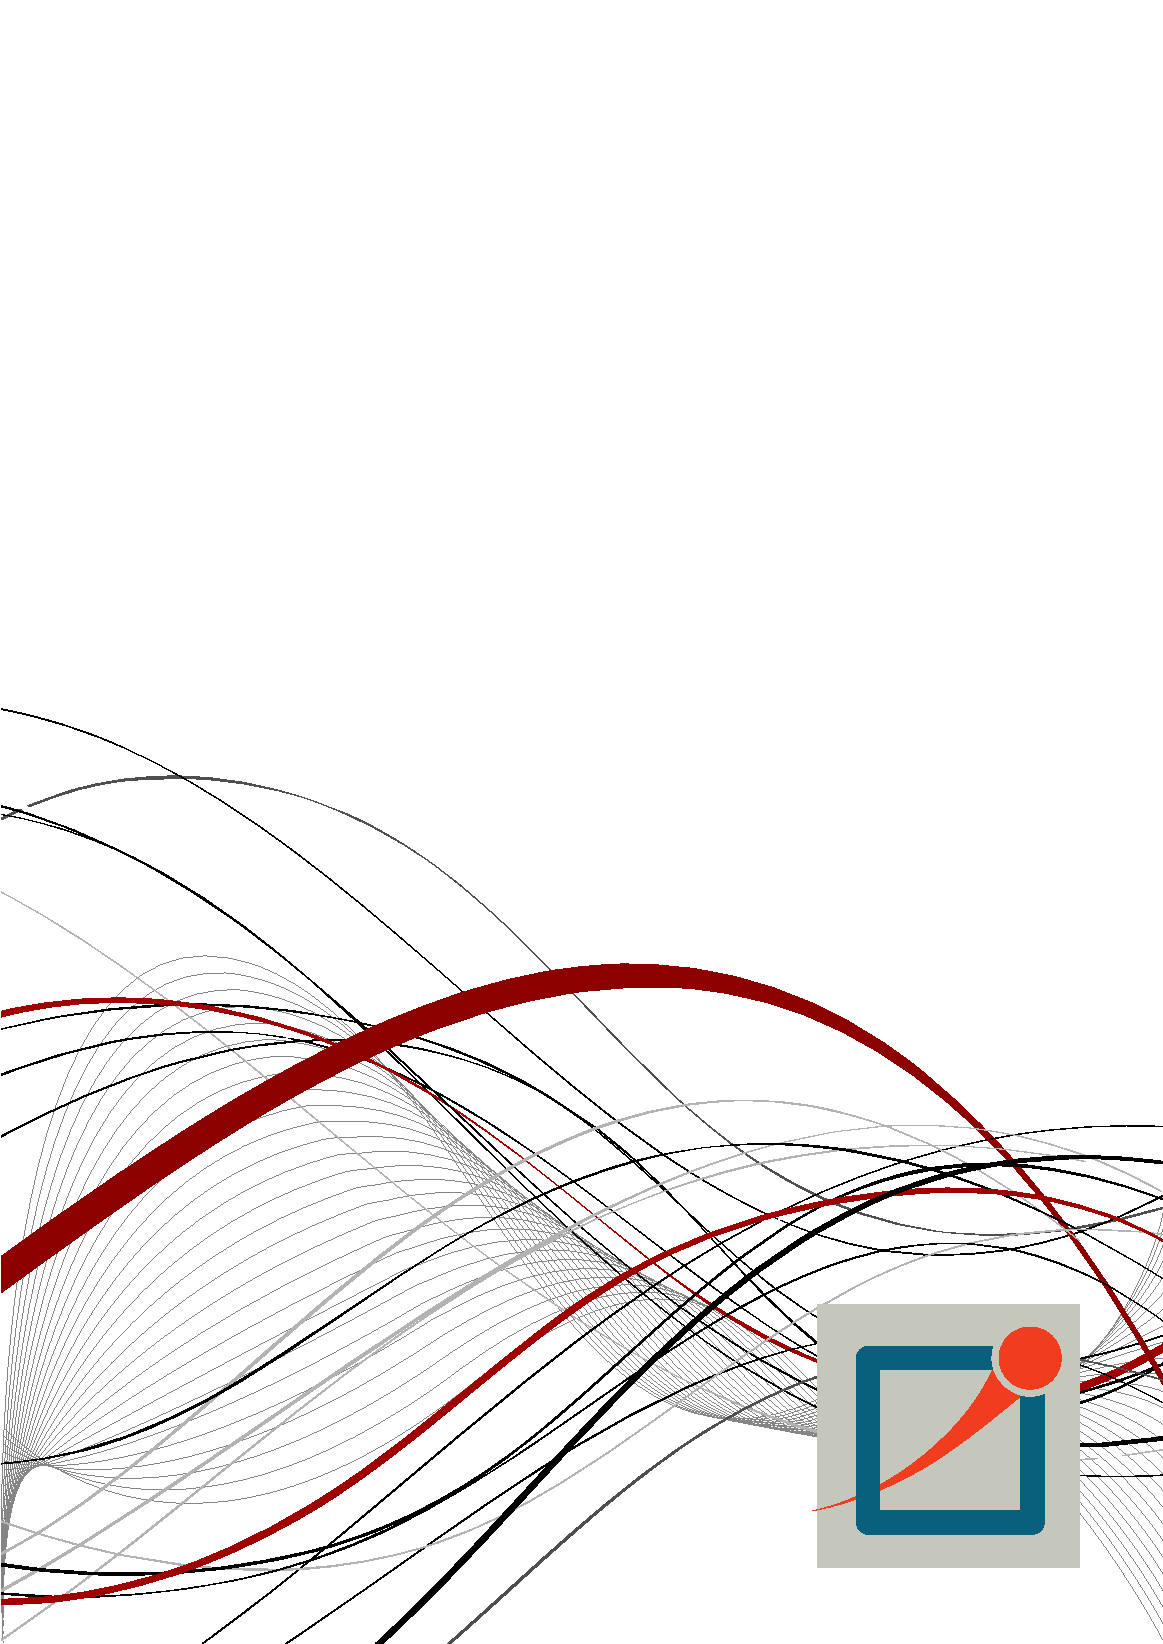
\includegraphics[width=\paperwidth,height=\paperheight]{../cover/cover-background.pdf}}
}
%% the following {center} is a trick -- vspace does nothing if there's
%% nothing above it in the page
\begin{center}\end{center}
\vspace{4cm}
\textbf{\fontsize{60}{80}\selectfont {\opp}}\par
\vspace{0.25cm}
{\fontsize{36}{50}\selectfont Simulation Manual}\par
{\LARGE Version {\oppversion}\par}
\vfill
\newpage
Copyright \copyright 1992-2021, Andr\'{a}s Varga and OpenSim Ltd.\par
\newpage
\cleardoublepage

%%\setcounter{page}{1}
%\newpage
%%\pagenumbering{roman}

\shorttableofcontents{Chapters}{0}
\cleardoublepage

\tableofcontents
\cleardoublepage

\pagestyle{fancy}
\pagenumbering{arabic}

%% XXX the following would set sans serif font: \sffamily

\include{ch-introduction}
\cleardoublepage

\include{ch-overview}
\cleardoublepage

\chapter{The NED Language}
\label{cha:ned-lang}


\section{NED Overview}
\label{sec:ned-lang:ned-overview}

The user describes the structure of a simulation model in the NED language. NED
stands for Network Description. NED lets the user declare simple modules, and
connect and assemble them into compound modules. The user can label some compound
modules as \textit{networks}; that is, self-contained simulation models. Channels are
another component type, whose instances can also be used in compound modules.

The NED language has several features which let it scale well to large projects:

\begin{description}

\item[Hierarchical.] The traditional way to deal with complexity is by
introducing hierarchies. In {\opp}, any module which would be too complex as
a single entity can be broken down into smaller modules, and used as a
compound module.

\item[Component-Based.] Simple modules and compound modules are inherently
reusable, which not only reduces code copying, but more importantly, allows
component libraries (like the INET Framework, MiXiM, Castalia, etc.) to
exist.

\item[Interfaces.] Module and channel interfaces can be used as a
placeholder where normally a module or channel type would be used, and the
concrete module or channel type is determined at network setup time by a
parameter. Concrete module types have to ``implement'' the interface they
can substitute. For example, given a compound module type named
\ttt{MobileHost} contains a \ttt{mobility} submodule of the type
\ttt{IMobility} (where \ttt{IMobility} is a module interface), the actual
type of \ttt{mobility} may be chosen from the module types that implemented
\ttt{IMobility} (\ttt{RandomWalkMobility}, \ttt{TurtleMobility}, etc.)

\item[Inheritance.] Modules and channels can be subclassed. Derived modules
and channels may add new parameters, gates, and (in the case of compound
modules) new submodules and connections. They may set existing parameters
to a specific value, and also set the gate size of a gate vector. This
makes it possible, for example, to take a \ttt{GenericTCPClientApp} module
and derive an \ttt{FTPClientApp} from it by setting certain parameters to a fixed
value; or to derive a \ttt{WebClientHost} compound module from a
\ttt{BaseHost} compound module by adding a \ttt{WebClientApp} submodule and
connecting it to the inherited \ttt{TCP} submodule.

\item[Packages.] The NED language features a Java-like package structure,
to reduce the risk of name clashes between different models. \ttt{NEDPATH}
(similar to Java's \ttt{CLASSPATH}) has also been introduced to make it easier
to specify dependencies among simulation models.

\item[Inner types.] Channel types and module types used locally by a
compound module can be defined within the compound module, in order to
reduce namespace pollution.

\item[Metadata annotations.] It is possible to annotate module or channel
types, parameters, gates and submodules by adding properties. Metadata are
not used by the simulation kernel directly, but they can carry extra
information for various tools, the runtime environment, or even for other
modules in the model. For example, a module's graphical representation
(icon, etc)  or the prompt string and measurement unit (milliwatt, etc) of a
parameter are already specified as metadata annotations.

\end{description}

\begin{note}
    The NED language has changed significantly in the 4.0 version.
    Inheritance, interfaces, packages, inner types, metadata annotations, inout
    gates were all added in the 4.0 release, together with many other features.
    Since the basic syntax has changed as well, old NED files need to be
    converted to the new syntax. There are automated tools for this purpose, so
    manual editing is only needed to take advantage of new NED features.
\end{note}

The NED language has an equivalent tree representation which can be
serialized to XML; that is, NED files can be converted to XML and back
without loss of data, including comments. This lowers the barrier for
programmatic manipulation of NED files; for example extracting information,
refactoring and transforming NED, generating NED from information stored in
other systems like SQL databases, and so on.

\begin{note}
    This chapter is going to explain the NED language gradually, via examples.
    A more formal and concise treatment can be found in Appendix \ref{cha:ned-language-grammar}.
\end{note}


\section{NED Quickstart}
\label{sec:ned-lang:warmup}

In this section we introduce the NED language via a complete and
reasonably real-life example: a communication network.

Our hypothetical network consists of nodes. On each node there is an
application running which generates packets at random intervals.
The nodes are routers themselves as well. We assume that the application
uses datagram-based communication, so that we can leave out the
transport layer from the model.


\subsection{The Network}
\label{sec:ned-lang:warmup:network}

First we'll define the network, then in the next sections we'll continue
to define the network nodes.

Let the network topology be as in Figure \ref{fig:ned-routing-topology}.

\begin{figure}[htbp]
  \begin{center}
    \includepng[scale=0.6]{figures/ned-routing-network}
    \caption{The network}
    \label{fig:ned-routing-topology}
  \end{center}
\end{figure}

The corresponding NED description would look like this:

\begin{ned}
//
// A network
//
network Network
{
    submodules:
        node1: Node;
        node2: Node;
        node3: Node;
        ...
    connections:
        node1.port++ <--> {datarate=100Mbps;} <--> node2.port++;
        node2.port++ <--> {datarate=100Mbps;} <--> node4.port++;
        node4.port++ <--> {datarate=100Mbps;} <--> node6.port++;
        ...
}
\end{ned}

The above code defines a network type named \ttt{Network}. Note that the NED
language uses the familiar curly brace syntax, and ``\ttt{//}'' to denote
comments.

\begin{note}
    Comments in NED not only make the source code more readable, but in the
    {\opp} IDE they also are displayed at various places (tooltips, content
    assist, etc), and become part of the documentation extracted from the NED
    files. The NED documentation system, not unlike \textit{JavaDoc} or
    \textit{Doxygen}, will be described in Chapter \ref{cha:neddoc}.
\end{note}

The network contains several nodes, named \ttt{node1}, \ttt{node2}, etc.
from the NED module type \ttt{Node}. We'll define \ttt{Node} in the next
sections.

The second half of the declaration defines how the nodes are to be
connected. The double arrow means bidirectional connection. The connection
points of modules are called gates, and the \ttt{port++} notation adds a
new gate to the \ttt{port[]} gate vector. Gates and connections will be
covered in more detail in sections \ref{sec:ned-lang:gates} and
\ref{sec:ned-lang:connections}. Nodes are connected with a channel that
has a data rate of 100Mbps.

\begin{note}
    In many other systems, the equivalent of {\opp} gates are called
    \textit{ports}. We have retained the term \textit{gate} to reduce
    collisions with other uses of the otherwise overloaded word
    \textit{port}: router port, TCP port, I/O port, etc.
\end{note}

The above code would be placed into a file named \ttt{Net6.ned}. It is
a convention to put every NED definition into its own file and to name the
file accordingly, but it is not mandatory to do so.

One can define any number of networks in the NED files, and for every
simulation the user has to specify which network to set up.
The usual way of specifying the network is to put the \fconfig{network}
option into the configuration (by default the \ffilename{omnetpp.ini} file):

\begin{inifile}
[General]
network = Network
\end{inifile}


\subsection{Introducing a Channel}
\label{sec:ned-lang:warmup:introducing-a-channel}

It is cumbersome to have to repeat the data rate for every connection.
Luckily, NED provides a convenient solution: one can create a new channel
type that encapsulates the data rate setting, and this channel type can
be defined inside the network so that it does not litter the global
namespace.

The improved network will look like this:

\begin{ned}
//
// A Network
//
network Network
{
    types:
        channel C extends ned.DatarateChannel {
            datarate = 100Mbps;
        }
    submodules:
        node1: Node;
        node2: Node;
        node3: Node;
        ...
    connections:
        node1.port++ <--> C <--> node2.port++;
        node2.port++ <--> C <--> node4.port++;
        node4.port++ <--> C <--> node6.port++;
        ...
}
\end{ned}

Later sections will cover the concepts used (inner types, channels, the
\ttt{DatarateChannel} built-in type, inheritance) in detail.


\subsection{The App, Routing, and Queue Simple Modules}
\label{sec:ned-lang:warmup:the-simple-modules}

Simple modules are the basic building blocks for other (compound) modules,
denoted by the \fkeyword{simple} keyword.
All active behavior in the model is encapsulated in \fkeyword{simple} modules.
Behavior is defined with a C++ class; NED files only declare the externally
visible interface of the module (gates, parameters).

In our example, we could define \ttt{Node} as a simple module. However,
its functionality is quite complex (traffic generation, routing, etc),
so it is better to implement it with several smaller simple module types
which we are going to assemble into a compound module. We'll have
one simple module for traffic generation (\ttt{App}), one for routing
(\ttt{Routing}), and one for queueing up packets to be sent out (\ttt{Queue}).
For brevity, we omit the bodies of the latter two in the code below.

\begin{ned}
simple App
{
    parameters:
        int destAddress;
        ...
        @display("i=block/browser");
    gates:
        input in;
        output out;
}

simple Routing
{
    ...
}

simple Queue
{
    ...
}
\end{ned}

By convention, the above simple module declarations go into the
\ttt{App.ned}, \ttt{Routing.ned} and \ttt{Queue.ned} files.

\begin{note}
    Note that module type names (\ttt{App}, \ttt{Routing}, \ttt{Queue})
    begin with a capital letter, and parameter and gate names begin with
    lowercase -- this is the recommended naming convention. Capitalization
    matters because the language is case sensitive.
\end{note}

Let us look at the first simple module type declaration. \ttt{App} has a
parameter called \ttt{destAddress} (others have been omitted for now),
and two gates named \ttt{out} and \ttt{in} for sending and receiving
application packets.

The argument of \fprop{@display()} is called a \textit{display string},
and it defines the rendering of the module in graphical environments;
\ttt{"i=..."} defines the default icon.

Generally, \ttt{@}-words like \ttt{@display} are called \textit{properties}
in NED, and they are used to annotate various objects
with metadata. Properties can be attached to files, modules, parameters, gates,
connections, and other objects, and parameter values have a very flexible
syntax.


\subsection{The Node Compound Module}
\label{sec:warmup:ned-lang:node-compound-module}

Now we can assemble \ttt{App}, \ttt{Routing} and \ttt{Queue} into the
compound module \ttt{Node}. A compound module can be thought of as
a ``cardboard box'' that groups other modules into a larger unit,
which can further be used as a building block for other modules;
networks are also a kind of compound module.

\begin{figure}[htbp]
  \begin{center}
    \includepng[scale=0.6]{figures/ned-routing-node}
    \caption{The Node compound module}
    \label{fig:ned-routing-node}
  \end{center}
\end{figure}

\begin{ned}
module Node
{
    parameters:
        int address;
        @display("i=misc/node_vs,gold");
    gates:
        inout port[];
    submodules:
        app: App;
        routing: Routing;
        queue[sizeof(port)]: Queue;
    connections:
        routing.localOut --> app.in;
        routing.localIn <-- app.out;
        for i=0..sizeof(port)-1 {
            routing.out[i] --> queue[i].in;
            routing.in[i] <-- queue[i].out;
            queue[i].line <--> port[i];
        }
}
\end{ned}

Compound modules, like simple modules, may have parameters and gates.
Our \ttt{Node} module contains an \ttt{address} parameter, plus a
\textit{gate vector} of unspecified size, named \ttt{port}.
The actual gate vector size will be determined implicitly by the number
of neighbours when we create a network from nodes of this type.
The type of \ttt{port[]} is \ttt{inout}, which allows bidirectional
connections.

The modules that make up the compound module are listed under
\fkeyword{submodules}. Our \ttt{Node} compound module type has an \ttt{app} and
a \ttt{routing} \textit{submodule}, plus a \ttt{queue[]} \textit{submodule
vector} that contains one \ttt{Queue} module for each port, as specified by
\ttt{[sizeof(port)]}. (It is legal to refer to \ttt{[sizeof(port)]} because
the network is built in top-down order, and the node is already created and
connected at network level when its submodule structure is built out.)

In the \fkeyword{connections} section, the submodules are connected to each
other and to the parent module. Single arrows are used to connect input and
output gates, and double arrows connect inout gates, and a \fkeyword{for} loop
is utilized to connect the \ttt{routing} module to each \ttt{queue} module, and
to connect the outgoing/incoming link (\ttt{line} gate) of each queue to the
corresponding port of the enclosing module.


\subsection{Putting It Together}
\label{sec:ned-lang:warmup:putting-it-together}

We have created the NED definitions for this example, but how are they used by {\opp}? When
the simulation program is started, it loads the NED files. The program
should already contain the C++ classes that implement the needed simple
modules, \ttt{App}, \ttt{Routing} and \ttt{Queue}; their C++ code is either
part of the executable or is loaded from a shared library. The simulation
program also loads the configuration (\ffilename{omnetpp.ini}), and determines
from it that the simulation model to be run is the \ttt{Network} network.
Then the network is instantiated for simulation.

The simulation model is built in a top-down preorder fashion. This means
that starting from an empty system module, all submodules are created,
their parameters and gate vector sizes are assigned, and they are fully connected
before the submodule internals are built.

\bigskip
\begin{center}
* * *
\end{center}
\bigskip

In the following sections we'll go through the elements of the NED
language and look at them in more detail.



\section{Simple Modules}
\label{sec:ned-lang:simple-modules}

Simple modules are the active components in the model.
Simple modules are defined with the \fkeyword{simple} keyword.

An example simple module:

\begin{ned}
simple Queue
{
    parameters:
        int capacity;
        @display("i=block/queue");
    gates:
        input in;
        output out;
}
\end{ned}

Both the \fkeyword{parameters} and \fkeyword{gates} sections are optional, that is,
they can be left out if there is no parameter or gate. In addition, the
\fkeyword{parameters} keyword itself is optional too; it can be left out
even if there are parameters or properties.

Note that the NED definition doesn't contain any code to define the
operation of the module: that part is expressed in C++. By default, {\opp}
looks for C++ classes of the same name as the NED type (so here, \ttt{Queue}).

One can explicitly specify the C++ class with the \fprop{@class} property.
Classes with namespace qualifiers are also accepted, as shown in the following
example that uses the \ttt{mylib::Queue} class:

\begin{ned}
simple Queue
{
    parameters:
        int capacity;
        @class(mylib::Queue);
        @display("i=block/queue");
    gates:
        input in;
        output out;
}
\end{ned}

If there are several modules whose C++ implementation classes are in the same
namespace, a better alternative to \fprop{@class} is the \fprop{@namespace} property.
The C++ namespace given with \fprop{@namespace} will be prepended to the normal
class name. In the following example, the C++ classes will be \ttt{mylib::App},
\ttt{mylib::Router} and \ttt{mylib::Queue}:

\begin{ned}
@namespace(mylib);

simple App {
   ...
}

simple Router {
   ...
}

simple Queue {
   ...
}
\end{ned}

The \fprop{@namespace} property may not only be specified at file level as
in the above example, but for packages as well. When placed in a file
called \ttt{package.ned}, the namespace will apply to all components in
that package and below.

The implementation C++ classes need to be subclassed from the
\cclass{cSimpleModule} library class; chapter \ref{cha:simple-modules} of
this manual describes in detail how to write them.

Simple modules can be extended (or specialized) via subclassing. The
motivation for subclassing can be to set some open parameters or gate sizes
to a fixed value (see \ref{sec:ned-lang:parameters} and
\ref{sec:ned-lang:gates}), or to replace the C++ class with a different
one. Now, by default, the derived NED module type will \textit{inherit} the
C++ class from its base, so it is important to remember that you need to
write out \fprop{@class} if you want it to use the new class.

The following example shows how to specialize a module by setting a parameter
to a fixed value (and leaving the C++ class unchanged):

\begin{ned}
simple Queue
{
   int capacity;
   ...
}

simple BoundedQueue extends Queue
{
   capacity = 10;
}
\end{ned}

In the next example, the author wrote a \ttt{PriorityQueue} C++ class, and
wants to have a corresponding NED type, derived from \ttt{Queue}. However,
it does not work as expected:

\begin{ned}
simple PriorityQueue extends Queue // wrong! still uses the Queue C++ class
{
}
\end{ned}

The correct solution is to add a \fprop{@class} property to override the
inherited C++ class:

\begin{ned}
simple PriorityQueue extends Queue
{
   @class(PriorityQueue);
}
\end{ned}

Inheritance in general will be discussed in section \ref{sec:ned-lang:inheritance}.



\section{Compound Modules}
\label{sec:ned-lang:compound-modules}

A compound module groups other modules into a larger unit. A compound
module may have gates and parameters like a simple module, but no active
behavior is associated with it.\footnote{Although the C++ class
for a compound module can be overridden with the \fprop{@class} property,
this is a feature that should probably never be used. Encapsulate the code
into a simple module, and add it as a submodule.}

\begin{note}
    When there is a temptation to add code to a compound module,
    then encapsulate the code into a simple module, and add it as
    a submodule.
\end{note}

A compound module declaration may contain several sections,
all of them optional:

\begin{ned}
module Host
{
   types:
       ...
   parameters:
       ...
   gates:
       ...
   submodules:
       ...
   connections:
       ...
}
\end{ned}

Modules contained in a compound module are called submodules, and they are
listed in the \ttt{submodules} section. One can create arrays of submodules
(i.e. submodule vectors), and the submodule type may come from a parameter.

Connections are listed under the \ttt{connections} section of the
declaration. One can create connections using simple programming constructs
(loop, conditional). Connection behaviour can be defined by associating a
channel with the connection; the channel type may also come from a
parameter.

Module and channel types only used locally can be defined in the
\ttt{types} section as inner types, so that they do not pollute the
namespace.

Compound modules may be extended via subclassing. Inheritance may add new
submodules and new connections as well, not only parameters and gates.
Also, one may refer to inherited submodules, to inherited types etc. What
is not possible is to "de-inherit" or modify submodules or connections.

In the following example, we show how to assemble common protocols
into a "stub" for wireless hosts, and add user agents via
subclassing.\footnote{Module types, gate names, etc. used in the example
are fictional, not based on an actual {\opp}-based model framework}

\begin{ned}
module WirelessHostBase
{
   gates:
       input radioIn;
   submodules:
       tcp: TCP;
       ip: IP;
       wlan: Ieee80211;
   connections:
       tcp.ipOut --> ip.tcpIn;
       tcp.ipIn <-- ip.tcpOut;
       ip.nicOut++ --> wlan.ipIn;
       ip.nicIn++ <-- wlan.ipOut;
       wlan.radioIn <-- radioIn;
}

module WirelessHost extends WirelessHostBase
{
   submodules:
       webAgent: WebAgent;
   connections:
       webAgent.tcpOut --> tcp.appIn++;
       webAgent.tcpIn <-- tcp.appOut++;
}
\end{ned}

The \ttt{WirelessHost} compound module can further be extended,
for example with an Ethernet port:

\begin{ned}
module DesktopHost extends WirelessHost
{
   gates:
       inout ethg;
   submodules:
       eth: EthernetNic;
   connections:
       ip.nicOut++ --> eth.ipIn;
       ip.nicIn++ <-- eth.ipOut;
       eth.phy <--> ethg;
}
\end{ned}



\section{Channels}
\label{sec:ned-lang:channels}

Channels encapsulate parameters and behaviour associated with connections.
Channels are like simple modules, in the sense that there are C++ classes
behind them. The rules for finding the C++ class for a NED channel type is
the same as with simple modules: the default class name is the NED type
name unless there is a \fprop{@class} property (\fprop{@namespace} is also
recognized), and the C++ class is inherited when the channel is subclassed.

Thus, the following channel type would expect a \ttt{CustomChannel} C++ class
to be present:

\begin{ned}
channel CustomChannel  // requires a CustomChannel C++ class
{
}
\end{ned}

The practical difference compared to modules is that one rarely needs to write
custom channel C++ class because there are predefined channel types that one can
subclass from, inheriting their C++ code. The predefined types are:
\ttt{ned.IdealChannel}, \ttt{ned.Delay\-Channel} and \ttt{ned.Datarate\-Channel}.
(``\ttt{ned}'' is the package name; one can get rid of it by importing the types
with the \ttt{import ned.*} directive. Packages and imports are described in
section \ref{sec:ned-lang:packages}.)

\ttt{IdealChannel} has no parameters, and lets through all messages without
delay or any side effect. A connection without a channel object
and a connection with an \ttt{IdealChannel} behave in the same way.
Still, \ttt{IdealChannel} has its uses, for example when a channel object
is required so that it can carry a new property or parameter that is
going to be read by other parts of the simulation model.

\ttt{DelayChannel} has two parameters:

\begin{itemize}
    \item \ttt{delay} is a \ttt{double} parameter which represents the
          propagation delay of the message. Values need to be specified
          together with a time unit (\ttt{s}, \ttt{ms}, \ttt{us}, etc.)
    \item \ttt{disabled} is a boolean parameter that defaults to \ttt{false};
          when set to \ttt{true}, the channel object will drop all messages.
\end{itemize}

\ttt{DatarateChannel} has a few additional parameters compared to \ttt{DelayChannel}:

\begin{itemize}
    \item \ttt{datarate} is a \ttt{double} parameter that represents the
          data rate of the channel. Values need to be specified
          in bits per second or its multiples as unit (\ttt{bps},
          \ttt{kbps}, \ttt{Mbps}, \ttt{Gbps}, etc.) Zero is treated
          specially and results in zero transmission duration, i.e.
          it stands for infinite bandwidth. Zero is also the default.
          Data rate is used for calculating the transmission duration of
          packets.
    \item \ttt{ber} and \ttt{per} stand for Bit Error Rate and Packet Error Rate,
          and allow basic error modelling. They expect a \ttt{double}
          in the $[0,1]$ range. When the channel decides (based on random
          numbers) that an error occurred during transmission of a packet,
          it sets an error flag in the packet object. The receiver
          module is expected to check the flag, and discard the packet
          as corrupted if it is set. The default \ttt{ber} and \ttt{per}
          are zero.
\end{itemize}

\begin{note}
    There is no channel parameter that specifies whether the channel
    delivers the message object to the destination module at the end or
    at the start of the reception; that is decided by the C++ code
    of the target simple module. See the \ffunc{setDeliverOn\-Reception\-Start()}
    method of \cclass{cGate}.
\end{note}

The following example shows how to create a new channel type by
specializing \ttt{DatarateChannel}:

\begin{ned}
channel Ethernet100 extends ned.DatarateChannel
{
    datarate = 100Mbps;
    delay = 100us;
    ber = 1e-10;
}
\end{ned}

\begin{note}
    The three built-in channel types are also used for connections where
    the channel type is not explicitly specified.
\end{note}

One may add parameters and properties to channels via subclassing, and
may modify existing ones. In the following example, we introduce distance-based
calculation of the propagation delay:

\begin{ned}
channel DatarateChannel2 extends ned.DatarateChannel
{
    double distance @unit(m);
    delay = this.distance / 200000km * 1s;
}
\end{ned}

Parameters are primarily intended to be read by the underlying C++ class,
but new parameters may also be added as annotations to be used by other
parts of the model. For example, a \ttt{cost} parameter may be used for
routing decisions in routing module, as shown in the example below. The
example also shows annotation using properties (\fprop{@backbone}).

\begin{ned}
channel Backbone extends ned.DatarateChannel
{
    @backbone;
    double cost = default(1);
}
\end{ned}


\section{Parameters}
\label{sec:ned-lang:parameters}

Parameters are variables that belong to a module. Parameters can be
used in building the topology (number of nodes, etc), and to supply
input to C++ code that implements simple modules and channels.

Parameters can be of type \fkeyword{double}, \fkeyword{int},
\fkeyword{bool}, \fkeyword{string}, \fkeyword{xml} and \fkeyword{object};
they can also be declared \fkeyword{volatile}. For the numeric types, a unit of
measurement can also be specified (\fprop{@unit} property).

Parameters can get their value from NED files or from the configuration
(\ffilename{omnetpp.ini}). A default value can also be given (\ttt{default(}...\ttt{)}),
which is used if the parameter is not assigned otherwise.

The following example shows a simple module that has five parameters, three
of which have default values:

\begin{ned}
simple App
{
    parameters:
        string protocol;       // protocol to use: "UDP" / "IP" / "ICMP" / ...
        int destAddress;       // destination address
        volatile double sendInterval @unit(s) = default(exponential(1s));
                               // time between generating packets
        volatile int packetLength @unit(byte) = default(100B);
                               // length of one packet
        volatile int timeToLive = default(32);
                               // maximum number of network hops to survive
    gates:
        input in;
        output out;
}
\end{ned}


\subsection{Assigning a Value}
\label{sec:ned-lang:parameter-assignments}

Parameters may get their values in several ways: from NED code, from the
configuration (\ffilename{omnetpp.ini}), or even, interactively from the
user. NED lets one assign parameters at several places: in subclasses via
inheritance; in submodule and connection definitions where the NED type is
instantiated; and in networks and compound modules that directly or
indirectly contain the corresponding submodule or connection.

For instance, one could specialize the above \ttt{App} module type via
inheritance with the following definition:

\begin{ned}
simple PingApp extends App
{
    parameters:
        protocol = "ICMP/ECHO"
        sendInterval = default(1s);
        packetLength = default(64byte);
}
\end{ned}

This definition sets the \ttt{protocol} parameter to a fixed value
(\ttt{"ICMP/ECHO"}), and changes the default values of the
\ttt{sendInterval} and \ttt{packetLength} parameters. \ttt{protocol} is now
locked down in \ttt{PingApp}, its value cannot be modified via further subclassing
or other ways. \ttt{sendInterval} and \ttt{packetLength} are still unassigned
here, only their default values have been overwritten.

Now, let us see the definition of a \ttt{Host} compound module that uses
\ttt{PingApp} as submodule:

\begin{ned}
module Host
{
    submodules:
        ping : PingApp {
            packetLength = 128B; // always ping with 128-byte packets
        }
        ...
}
\end{ned}

This definition sets the \ttt{packetLength} parameter to a fixed value. It
is now hardcoded that \ttt{Host}s send 128-byte ping packets; this
setting cannot be changed from NED or the configuration.

It is not only possible to set a parameter from the compound module that
contains the submodule, but also from modules higher up in the module tree.
A network that employs several \ttt{Host} modules could be defined like
this:

\begin{ned}
network Network
{
    submodules:
        host[100]: Host {
            ping.timeToLive = default(3);
            ping.destAddress = default(0);
        }
        ...
}
\end{ned}

Parameter assignment can also be placed into the \ttt{parameters} block of
the parent compound module, which provides additional flexibility. The
following definition sets up the hosts so that half of them pings host \#50,
and the other half pings host \#0:

\begin{ned}
network Network
{
    parameters:
        host[*].ping.timeToLive = default(3);
        host[0..49].ping.destAddress = default(50);
        host[50..].ping.destAddress = default(0);

    submodules:
        host[100]: Host;
        ...
}
\end{ned}

Note the use of asterisk to match any index, and \ttt{..} to match index ranges.

If there were a number of individual hosts instead of a submodule vector,
the network definition could look like this:

\begin{ned}
network Network
{
    parameters:
        host*.ping.timeToLive = default(3);
        host{0..49}.ping.destAddress = default(50);
        host{50..}.ping.destAddress = default(0);

    submodules:
        host0: Host;
        host1: Host;
        host2: Host;
        ...
        host99: Host;
}
\end{ned}

An asterisk matches any substring not containing a dot, and a \ttt{..}
within a pair of curly braces matches a natural number embedded in a
string.

In most assigments we have seen above, the left hand side of the equal sign
contained a dot and often a wildcard as well (asterisk or numeric range);
we call these assignments \textit{pattern assignments} or \textit{deep
assignments}.

There is one more wildcard that can be used in pattern assignments, and
this is the double asterisk; it matches any sequence of characters
including dots, so it can match multiple path elements. An example:

\begin{ned}
network Network
{
    parameters:
        **.timeToLive = default(3);
        **.destAddress = default(0);
    submodules:
        host0: Host;
        host1: Host;
        ...
}
\end{ned}

Note that some assignments in the above examples changed default values,
while others set parameters to fixed values. Parameters that received no
fixed value in the NED files can be assigned from the configuration
(\ffilename{omnetpp.ini}).

\begin{important}
    A non-default value assigned from NED cannot be overwritten later in
    NED or from ini files; it becomes ``hardcoded'' as far as ini files
    and NED usage are concerned. In contrast, default values are possible
    to overwrite.
\end{important}

A parameter can be assigned in the configuration using a similar syntax as
NED pattern assignments (actually, it would be more historically accurate
to say it the other way round, that NED pattern assignments use a similar
syntax to ini files):

%% FIXME show patterns for channel parameters too!

\begin{inifile}
Network.host[*].ping.sendInterval = 500ms  # for the host[100] example
Network.host*.ping.sendInterval = 500ms    # for the host0,host1,... example
**.sendInterval = 500ms
\end{inifile}

One often uses the double asterisk to save typing. One can write

\begin{inifile}
**.ping.sendInterval = 500ms
\end{inifile}

Or if one is certain that only ping modules have \ttt{sendInterval} parameters,
the following will suffice:

\begin{inifile}
**.sendInterval = 500ms
\end{inifile}

Parameter assignments in the configuration are described in section
\ref{sec:config-sim:parameter-settings}.

One can also write expressions, including stochastic expressions, in
NED files and in ini files as well. For example, here's how one can
add jitter to the sending of ping packets:

\begin{inifile}
**.sendInterval = 1s + normal(0s, 0.001s)  # or just: normal(1s, 0.001s)
\end{inifile}

If there is no assignment for a parameter in NED or in the ini file, the
default value (given with \ttt{=default(...)} in NED) will be applied
implicitly. If there is no default value, the user will be asked, provided
the simulation program is allowed to do that; otherwise there will be an
error. (Interactive mode is typically disabled for batch executions where
it would do more harm than good.)

It is also possible to explicitly apply the default (this can sometimes
be useful):

\begin{inifile}
**.sendInterval = default
\end{inifile}

Finally, one can explicitly ask the simulator to prompt the user interactively
for the value (again, provided that interactivity is enabled; otherwise
this will result in an error):

\begin{inifile}
**.sendInterval = ask
\end{inifile}

\begin{note}
    How can one decide whether to assign a parameter from NED or from an ini
    file? The advantage of ini files is that they allow a cleaner separation of the \textit{model}
    and \textit{experiments}. NED files (together with C++ code) are considered
    to be part of the model, and to be more or less constant. Ini files, on
    the other hand, are for experimenting with the model by running it
    several times with different parameters. Thus, parameters that are expected
    to change (or make sense to be changed) during experimentation should be
    put into ini files.
\end{note}


\subsection{Expressions}
\label{sec:ned-lang:expressions}

Parameter values may be given with expressions. NED language expressions
have a C-like syntax, with some variations on operator names: binary and
logical XOR are \ttt{\#} and \ttt{\#\#}, while \ttt{\^} has been reassigned
to \textit{power-of} instead. The \ttt{+} operator does string
concatenation as well as numeric addition. Expressions can use various
numeric, string, stochastic and other functions (\ttt{fabs()}, \ttt{toUpper()},
\ttt{uniform()}, \ttt{erlang\_k()}, etc.).

\begin{note}
    The list of NED functions can be found in Appendix \ref{cha:ned-functions}.
    The user can also extend NED with new functions.
\end{note}

%% XXX also sources of random numbers

Expressions may refer to module parameters, gate vector and module vector sizes
(using the \fkeyword{sizeof} operator) and the index of the current module
in a submodule vector (\fkeyword{index}).

%% XXX note: fullPath() etc functions!

Expressions may refer to parameters of the compound module being defined,
of the current module (with the \ttt{this.} prefix), and to parameters
of already defined submodules, with the syntax \ttt{submodule.parametername}
(or \ttt{submodule[index].parametername}).

%% XXX example: address = address;  delay=this.distance/this.speed;

%% XXX there are no parameter arrays, but... demonstrate the choose() function


\subsection{volatile}
\label{sec:ned-lang:volatile}

The \fkeyword{volatile} modifier causes the parameter's value expression to
be evaluated every time the parameter is read. This has significance if the
expression is not constant, for example it involves numbers drawn from a
random number generator. In contrast, non-volatile parameters are evaluated
only once. (This practically means that they are evaluated and replaced
with the resulting constant at the start of the simulation.)

To better understand \fkeyword{volatile}, let's suppose we have a
\ttt{Queue} simple module that has a \ttt{volatile double} parameter
named \ttt{serviceTime}.

\begin{ned}
simple Queue
{
    parameters:
        volatile double serviceTime;
}
\end{ned}

Because of the \fkeyword{volatile} modifier, the queue module's C++
implementation is expected to re-read the \ttt{serviceTime} parameter
whenever a value is needed; that is, for every job serviced. Thus, if
\ttt{serviceTime} is assigned an expression like \ttt{uniform(0.5s, 1.5s)},
every job will have a different, random service time. To highlight this
effect, here's how one can have a time-varying parameter by exploiting
the \ttt{simTime()} NED function that returns the current simulation time:

\begin{inifile}
**.serviceTime = simTime()<1000s ? 1s : 2s  # queue that slows down after 1000s
\end{inifile}

In practice, a volatile parameters are typically used as a configurable
source of random numbers for modules.

\begin{note}
    This does not mean that a non-volatile parameter could not be assigned a
    random value like \ttt{uniform(0.5s, 1.5s)}. It can, but that would
    have a totally different effect: the simulation would use a constant
    service time, say \ttt{1.2975367s}, chosen randomly at the beginning
    of the simulation.
\end{note}

\subsection{Units}
\label{sec:ned-lang:units}

One can declare a parameter to have an associated unit of measurement,
by adding the \fprop{@unit} property. An example:

\begin{ned}
simple App
{
    parameters:
        volatile double sendInterval @unit(s) = default(exponential(350ms));
        volatile int packetLength @unit(byte) = default(4KiB);
    ...
}
\end{ned}

The \ttt{@unit(s)} and \ttt{@unit(byte)} declarations specify the measurement unit
for the parameter. Values assigned to parameters must have the same or
compatible unit, i.e. \ttt{@unit(s)} accepts milliseconds, nanoseconds,
minutes, hours, etc., and \ttt{@unit(byte)} accepts kilobytes, megabytes,
etc. as well.

\begin{note}
    The list of units accepted by {\opp} is listed in the Appendix, see
    \ref{sec:ned-ref:units}. Unknown units (\ttt{bogomips}, etc.)
    can also be used, but there are no conversions for them,
    i.e. decimal prefixes will not be recognized.
\end{note}

The {\opp} runtime does a full and rigorous unit check on
parameters to ensure ``unit safety'' of models. Constants should
always include the measurement unit.

The \fprop{@unit} property of a parameter cannot be added or overridden
in subclasses or in submodule declarations.


\subsection{XML Parameters}
\label{sec:ned-lang:xml-parameters}

{\opp} supports two explicit ways of passing structured data to a module using
parameters: XML parameters, and object parameters with JSON-style structured data.
This section describes the former, and the next one the latter.

XML parameters are declared with the keyword \fkeyword{xml}. When using
XML parameters, {\opp} will read the XML document for you, DTD-validates it
(if it contains a DOCTYPE), and presents the contents in a DOM-like object tree.
It is also possible to assign a part (i.e. subtree) of the document to the parameter; the
subset can be selected using an XPath-subset notation. {\opp} caches the
content of the document, so it is loaded only once even if it is referenced
by multiple parameters.

Values for an XML parameter can be produced using the \fkeyword{xmldoc()} and
the \fkeyword{xml()} functions. \fkeyword{xmldoc()} accepts a filename as argument,
while \fkeyword{xml()} parses its string argument as XML content.
Of course, one can assign \fkeyword{xml} parameters both from NED and
from \ffilename{omnetpp.ini}.

The following example declares an \fkeyword{xml} parameter, and assigns the
contents of an XML file to it. The file name is understood as being relative
to the working directory.

\begin{ned}
simple TrafGen {
    parameters:
        xml profile;
    gates:
        output out;
}

module Node {
    submodules:
        trafGen1 : TrafGen {
            profile = xmldoc("data.xml");
        }
        ...
}
\end{ned}

\fkeyword{xmldoc()} also lets one select an element \textit{within} an XML
document. In case a simulation model contains numerous modules that need XML
input, this feature allows the user get rid of the many small XML files
by aggregating them into a single XML file. For example, the
following XML file contains two profiles identified with the IDs
\textit{gen1} and \textit{gen2}:

\begin{filelisting}
<?xml>
<root>
    <profile id="gen1">
          <param>3</param>
          <param>5</param>
    </profile>
    <profile id="gen2">
          <param>9</param>
    </profile>
</root>
\end{filelisting}

And one can assign each profile to a corresponding submodule using an XPath-like
expression:

\begin{ned}
module Node {
    submodules:
        trafGen1 : TrafGen {
            profile = xmldoc("all.xml", "/root/profile[@id='gen1']");
        }
        trafGen2 : TrafGen {
            profile = xmldoc("all.xml", "/root/profile[@id='gen2']");
        }
}
\end{ned}

The following example shows how specify XML content using a string literal,
with the \fkeyword{xml()} function. This is especially useful
for specifying a default value.

\begin{ned}
simple TrafGen {
    parameters:
        xml profile = xml("<root/>"); // empty document as default
        ...
}
\end{ned}

The \fkeyword{xml()} function, like \fkeyword{xmldoc()}, also supports an
optional second XPath parameter for selecting a subtree.

%% XXX other xmldoc syntax (=PARENTMODULEINDEX etc)


\subsection{Object/JSON Parameters}
\label{sec:ned-lang:object-parameters}

TODO

\section{Gates}
\label{sec:ned-lang:gates}

Gates are the connection points of modules.  {\opp} has three types of
gates: \textit{input}, \textit{output} and \textit{inout}, the latter being
essentially an input and an output gate glued together.

A gate, whether input or output, can only be connected to one other
gate. (For compound module gates, this means one connection ``outside'' and
one ``inside''.)  It is possible, though generally not recommended, to
connect the input and output sides of an inout gate separately (see section
\ref{sec:ned-lang:connections}).

One can create single gates and gate vectors. The size of a gate vector
can be given inside square brackets in the declaration, but it is also possible
to leave it open by just writing a pair of empty brackets (``\ttt{[]}'').

When the gate vector size is left open, one can still specify it later,
when subclassing the module, or when using the module for a submodule in a
compound module. However, it does not need to be specified because
one can create connections with the \ttt{$gate$++} operator that
automatically expands the gate vector.

The gate size can be queried from various NED expressions with the
\ttt{sizeof()} operator.

NED normally requires that all gates be connected. To relax this
requirement, one can annotate selected gates with the \fprop{@loose}
property, which turns off the connectivity check for that gate. Also, input
gates that solely exist so that the module can receive messages via
\ffunc{sendDirect()} (see \ref{sec:simple-modules:direct-sending}) should
be annotated with \fprop{@directIn}. It is also possible to turn off the connectivity
check for all gates within a compound module by specifying the
\fkeyword{allowunconnected} keyword in the module's connections section.

Let us see some examples.

In the following example, the \ttt{Classifier} module has one input for
receiving jobs, which it will send to one of the outputs. The number of
outputs is determined by a module parameter:

\begin{ned}
simple Classifier {
    parameters:
        int numCategories;
    gates:
        input in;
        output out[numCategories];
}
\end{ned}

The following \ttt{Sink} module also has its \ttt{in[]} gate defined
as a vector, so that it can be connected to several modules:

\begin{ned}
simple Sink {
    gates:
        input in[];
}
\end{ned}

The following lines define a node for building a square grid. Gates around
the edges of the grid are expected to remain unconnected, hence the
\fprop{@loose} annotation:

\begin{ned}
simple GridNode {
    gates:
        inout neighbour[4] @loose;
}
\end{ned}

\ttt{WirelessNode} below is expected to receive messages (radio transmissions)
via direct sending, so its \ttt{radioIn} gate is marked with \fprop{@directIn}.

\begin{ned}
simple WirelessNode {
    gates:
        input radioIn @directIn;
}
\end{ned}

In the following example, we define \ttt{TreeNode} as having gates to connect
any number of children, then subclass it to get a \ttt{BinaryTreeNode} to
set the gate size to two:

\begin{ned}
simple TreeNode {
    gates:
        inout parent;
        inout children[];
}

simple BinaryTreeNode extends TreeNode {
    gates:
        children[2];
}
\end{ned}

An example for setting the gate vector size in a submodule, using the same
\ttt{TreeNode} module type as above:

\begin{ned}
module BinaryTree {
    submodules:
        nodes[31]: TreeNode {
            gates:
                children[2];
        }
    connections:
        ...
}
\end{ned}



\section{Submodules}
\label{sec:ned-lang:submodules}

Modules that a compound module is composed of are called its submodules.
A submodule has a name, and it is an instance of a compound or simple
module type. In the NED definition of a submodule, this module type
is usually given statically, but it is also possible to specify the type
with a string expression. (The latter feature, \textit{parametric submodule
types}, will be discussed in section \ref{sec:ned-lang:submodule-like}.)

NED supports submodule arrays (vectors) and conditional submodules as well.
Submodule vector size, unlike gate vector size, must always be specified
and cannot be left open as with gates.

It is possible to add new submodules to an existing compound module via
subclassing; this has been described in the section
\ref{sec:ned-lang:compound-modules}.

The basic syntax of submodules is shown below:

\begin{ned}
module Node
{
    submodules:
        routing: Routing;   // a submodule
        queue[sizeof(port)]: Queue;  // submodule vector
        ...
}
\end{ned}

As already seen in previous code examples, a submodule may also have a
curly brace block as body, where one can assign parameters, set the size of
gate vectors, and add/modify properties like the display string
(\fprop{@display}). It is not possible to add new parameters and gates.

Display strings specified here will be merged with the display string
from the type to get the effective display string. The merge algorithm is
described in chapter \ref{cha:graphics}.

\begin{ned}
module Node
{
    gates:
        inout port[];
    submodules:
        routing: Routing {
            parameters:   // this keyword is optional
                routingTable = "routingtable.txt"; // assign parameter
            gates:
                in[sizeof(port)];  // set gate vector size
                out[sizeof(port)];
        }
        queue[sizeof(port)]: Queue {
            @display("t=queue id $id"); // modify display string
            id = 1000+index;  // use submodule index to generate different IDs
        }
    connections:
        ...
}
\end{ned}

An empty body may be omitted, that is,

\begin{ned}
      queue: Queue;
\end{ned}

is the same as

\begin{ned}
      queue: Queue {
      }
\end{ned}

A submodule or submodule vector can be conditional. The \fkeyword{if}
keyword and the condition itself goes after the submodule type, like in the
example below:

\begin{ned}
module Host
{
    parameters:
        bool withTCP = default(true);
    submodules:
        tcp : TCP if withTCP;
        ...
}
\end{ned}

Note that with submodule vectors, setting zero vector size can be used as an
alternative to the \fkeyword{if} condition.

\section{Connections}
\label{sec:ned-lang:connections}

Connections are defined in the \fkeyword{connections} section of compound
modules. Connections cannot span across hierarchy levels; one can connect
two submodule gates, a submodule gate and the "inside" of the parent
(compound) module's gates, or two gates of the parent module (though this
is rarely useful), but it is not possible to connect to any gate outside the
parent module, or inside compound submodules.

Input and output gates are connected with a normal arrow, and inout gates
with a double-headed arrow ``\ttt{<-{}->}''. To connect the two gates
with a channel, use two arrows and put the channel specification in between.
The same syntax is used to add properties such as \fprop{@display} to the
connection.

Some examples have already been shown in the NED Quickstart section
(\ref{sec:ned-lang:warmup}); let's see some more.

%% XXX examples

%% XXX explain \$i / \$o

It has been mentioned that an inout gate is basically an input and an
output gate glued together. These sub-gates can also be addressed (and
connected) individually if needed, as \ttt{port\$i} and \ttt{port\$o} (or
for vector gates, as \ttt{port\$i[$k$]} and \ttt{port\$o[$k$]}).

%% XXX explain ++

Gates are specified as \textit{modulespec.gatespec} (to connect a submodule),
or as \textit{gatespec} (to connect the compound module). \textit{modulespec}
is either a submodule name (for scalar submodules), or a submodule name plus
an index in square brackets (for submodule vectors). For scalar gates,
\textit{gatespec} is the gate name; for gate vectors it is either the gate name
plus an index in square brackets, or \textit{gatename}\ttt{++}.

The \textit{gatename}\ttt{++} notation causes the first unconnected gate index
to be used. If all gates of the given gate vector are connected, the behavior
is different for submodules and for the enclosing compound module.
For submodules, the gate vector expands by one. For a compound module,
after the last gate is connected, \ttt{++} will stop with an error.

\begin{note}
    Why is it not possible to expand a gate vector of the compound
    module? The model structure is built in top-down order, so new gates
    would be left unconnected on the outside, as there is no way in NED to
    "go back" and connect them afterwards.
\end{note}

When the \ttt{++} operator is used with \ttt{\$i} or \ttt{\$o}
(e.g. \ttt{g\$i++} or \ttt{g\$o++}, see later), it will actually add
a gate pair (input+output) to maintain equal gate sizes for the two
directions.

%% XXX examples


\subsection{Channel Specification}
\label{sec:ned-lang:channel-specification}

Channel specifications (\ttt{-{}->$channelspec$-{}->} inside a connection)
are similar to submodules in many respect. Let's see some examples!

The following connections use two user-defined channel types,
\ttt{Ethernet100} and \ttt{Backbone}. The code shows the syntax
for assigning parameters (\ttt{cost} and \ttt{length}) and specifying
a display string (and NED properties in general):

\begin{ned}
a.g++ <--> Ethernet100 <--> b.g++;
a.g++ <--> Backbone {cost=100; length=52km; ber=1e-8;} <--> b.g++;
a.g++ <--> Backbone {@display("ls=green,2");} <--> b.g++;
\end{ned}

When using built-in channel types, the type name can be omitted; it
will be inferred from the parameter names.

\begin{ned}
a.g++ <--> {delay=10ms;} <--> b.g++;
a.g++ <--> {delay=10ms; ber=1e-8;} <--> b.g++;
a.g++ <--> {@display("ls=red");} <--> b.g++;
\end{ned}

If \ttt{datarate}, \ttt{ber} or \ttt{per} is assigned,
\ttt{ned.DatarateChannel} will be chosen. Otherwise, if \ttt{delay} or
\ttt{disabled} is present, it will be \ttt{ned.DelayChannel}; otherwise it
is \ttt{ned.IdealChannel}. Naturally, if other parameter names are assigned
in a connection without an explicit channel type, it will be an error (with
\textit{``ned.DelayChannel has no such parameter''} or similar message).

Connection parameters, similarly to submodule parameters, can also
be assigned using pattern assignments, albeit the channel names
to be matched with patterns are a little more complicated and less
convenient to use. A channel can be identified with the name of its
source gate plus the channel name; the channel name is currently always
\ttt{channel}. It is illustrated by the following example:

\begin{ned}
module Queueing
{
    parameters:
        source.out.channel.delay = 10ms;
        queue.out.channel.delay = 20ms;
    submodules:
        source: Source;
        queue: Queue;
        sink: Sink;
    connections:
        source.out --> ned.DelayChannel --> queue.in;
        queue.out --> ned.DelayChannel <--> sink.in;
\end{ned}

Using bidirectional connections is a bit trickier, because both
directions must be covered separately:

\begin{ned}
network Network
{
    parameters:
        hostA.g$o[0].channel.datarate = 100Mbps; // the A -> B connection
        hostB.g$o[0].channel.datarate = 100Mbps; // the B -> A connection
        hostA.g$o[1].channel.datarate = 1Gbps;   // the A -> C connection
        hostC.g$o[0].channel.datarate = 1Gbps;   // the C -> A connection
    submodules:
        hostA: Host;
        hostB: Host;
        hostC: Host;
    connections:
        hostA.g++ <--> ned.DatarateChannel <--> hostB.g++;
        hostA.g++ <--> ned.DatarateChannel <--> hostC.g++;
\end{ned}

Also, with the \ttt{++} syntax it is not always easy to figure out which
gate indices map to the connections one needs to configure. If connection
objects could be given names to override the default name
``\ttt{channel}'', that would make it easier to identify connections in
patterns. This feature is described in the next section.


\subsection{Channel Names}
\label{sec:ned-lang:channel-names}

The default name given to channel objects is \ttt{"channel"}. Since {\opp} 4.3
it is possible to specify the name explicitly, and also to override
the default name per channel type. The purpose of custom channel names is to make
addressing easier when channel parameters are assigned from ini files.

The syntax for naming a channel in a connection is similar to submodule syntax:
\textit{name: type}. Since both \textit{name} and \textit{type} are optional,
the colon must be there after \textit{name} even if \textit{type} is missing,
in order to remove the ambiguity.

Examples:

\begin{ned}
r1.pppg++ <--> eth1: EthernetChannel <--> r2.pppg++;
a.out --> foo: {delay=1ms;} --> b.in;
a.out --> bar: --> b.in;
\end{ned}

In the absence of an explicit name, the channel name comes from the
\ttt{@defaultname} property of the channel type if that exists.

\begin{ned}
channel Eth10G extends ned.DatarateChannel like IEth {
    @defaultname(eth10G);
}
\end{ned}

There's a catch with \ttt{@defaultname} though: if the channel type is
specified with a \ttt{**.$channel\-name$.liketype=} line in an ini file, then
the channel type's \ttt{@defaultname} cannot be used as \textit{channelname}
in that configuration line, because the channel type would only be known as a
result of using that very configuration line. To illustrate the problem,
consider the above \ttt{Eth10G} channel, and a compound module containing the
following connection:

\begin{ned}
r1.pppg++ <--> <> like IEth <--> r2.pppg++;
\end{ned}

Then consider the following inifile:

\begin{inifile}
**.eth10G.typename = "Eth10G"   # Won't match! The eth10G name would come from
                                #   the Eth10G type - catch-22!
**.channel.typename = "Eth10G"  # OK, as lookup assumes the name "channel"
**.eth10G.datarate = 10.01Gbps  # OK, channel already exists with name "eth10G"
\end{inifile}

The anomaly can be avoided by using an explicit channel name in the connection,
not using \ttt{@defaultname}, or by specifying the type via a module parameter
(e.g. writing \ttt{<param> like ...} instead of \ttt{<> like ...}).



\section{Multiple Connections}
\label{sec:ned-lang:multiple-connections}

Simple programming constructs (loop, conditional) allow creating
multiple connections easily.

%% XXX explain for; nesting; explain if;

This will be shown in the following examples.

\subsection{Examples}
\label{sec:ned-lang:multiple-connections-examples}

\subsubsection{Chain}
\label{sec:ned-lang:chain-example}

One can create a chain\index{chain} of modules like this:

\begin{ned}
module Chain
    parameters:
        int count;
    submodules:
        node[count] : Node {
            gates:
                port[2];
        }
    connections allowunconnected:
        for i = 0..count-2 {
            node[i].port[1] <--> node[i+1].port[0];
        }
}
\end{ned}


\subsubsection{Binary Tree}
\label{sec:ned-lang:binary-tree-example}

One can build a binary tree\index{binary tree} in the following way:

\begin{ned}
simple BinaryTreeNode {
    gates:
        inout left;
        inout right;
        inout parent;
}

module BinaryTree {
    parameters:
        int height;
    submodules:
        node[2^height-1]: BinaryTreeNode;
    connections allowunconnected:
        for i=0..2^(height-1)-2 {
            node[i].left <--> node[2*i+1].parent;
            node[i].right <--> node[2*i+2].parent;
        }
}
\end{ned}

Note that not every gate of the modules will be connected. By default,
an unconnected gate produces a run-time error message when the
simulation is started, but this error message is turned off here with
the \fkeyword{allowunconnected} modifier.
Consequently, it is the simple modules' responsibility not to send
on an unconnected gate.



\subsubsection{Random Graph}
\label{sec:ned-lang:random-graph-example}

Conditional connections can be used to generate random
topologies\index{topology!random}, for example. The following code
generates a random subgraph of a full graph:

\begin{ned}
module RandomGraph {
    parameters:
        int count;
        double connectedness; // 0.0<x<1.0
    submodules:
        node[count]: Node {
            gates:
                in[count];
                out[count];
        }
    connections allowunconnected:
        for i=0..count-1, for j=0..count-1 {
            node[i].out[j] --> node[j].in[i]
                if i!=j && uniform(0,1)<connectedness;
        }
}
\end{ned}

Note the use of the \fkeyword{allowunconnected} modifier
here too, to turn off error messages produced by the network setup code
for unconnected gates.


\subsection{Connection Patterns}
\label{sec:ned-lang:connection-design-patterns}

\index{module!compound!patterns}
\index{topology!patterns}

Several approaches can be used for creating complex topologies that have a
regular structure; three of them are described below.


\subsubsection{``Subgraph of a Full Graph''}
\label{sec:ned-lang:subgraph-of-full-graph}


This pattern takes a subset of the connections of a full graph.  A
condition is used to ``carve out'' the necessary interconnection from
the full graph:

\begin{ned}
for i=0..N-1, for j=0..N-1 {
    node[i].out[...] --> node[j].in[...] if condition(i,j);
}
\end{ned}

The RandomGraph compound module (presented earlier) is an example of
this pattern, but the pattern can generate any graph where an
appropriate $condition(i,j)$ can be formulated. For example,
when generating a tree\index{topology!tree} structure, the condition
would return whether node $j$ is a child of node $i$ or
vice versa.

Though this pattern is very general, its usage can be prohibitive if
the number of nodes $N$ is high and the graph is sparse (it has
much less than $N^2$ connections). The following
two patterns do not suffer from this drawback.


\subsubsection{``Connections of Each Node''}
\label{sec:ned-lang:connections-of-each-node}

The pattern loops through all nodes and creates the necessary
connections for each one. It can be generalized like this:

\begin{ned}
for i=0..Nnodes, for j=0..Nconns(i)-1 {
    node[i].out[j] --> node[rightNodeIndex(i,j)].in[j];
}
\end{ned}

The Hypercube\index{topology!hypercube} compound module (to be
presented later) is a clear example of this approach. BinaryTree can
also be regarded as an example of this pattern where the inner j loop
is unrolled.

The applicability of this pattern depends on how easily the $rightNodeIndex(i,j)$
function can be formulated.


\subsubsection{``Enumerate All Connections''}
\label{sec:ned-lang:enumerate-all-connections}


A third pattern is to list all connections within a loop:

\begin{ned}
for i=0..Nconnections-1 {
    node[leftNodeIndex(i)].out[...] --> node[rightNodeIndex(i)].in[...];
}
\end{ned}

This pattern can be used if $leftNodeIndex(i)$ and $rightNodeIndex(i)$
mapping functions can be sufficiently formulated.

The \ttt{Chain} module is an example of this approach where the mapping
functions are extremely simple: $leftNodeIndex(i)=i$ and $rightNodeIndex(i) = i+1$.
The pattern can also be used to create a random subset of a full
graph with a fixed number of connections.

In the case of irregular structures where none of the above patterns
can be employed, one can resort to listing all connections, like one
would do it in most existing simulators.



\section{Parametric Submodule and Connection Types}
\label{sec:ned-lang:parametric-submodule-and-connection-types}

\subsection{Parametric Submodule Types}
\label{sec:ned-lang:submodule-like}

A submodule type may be specified with a module parameter of the type
\fkeyword{string}, or in general, with any string-typed expression.
The syntax uses the \fkeyword{like} keyword.

Let us begin with an example:

\begin{ned}
network Net6
{
    parameters:
        string nodeType;
    submodules:
        node[6]: <nodeType> like INode {
            address = index;
        }
    connections:
        ...
}
\end{ned}

It creates a submodule vector whose module type will come from the
\ttt{nodeType} parameter. For example, if \ttt{nodeType} is set to \ttt{"SensorNode"},
then the module vector will consist of sensor nodes, provided such module
type exists and it qualifies. What this means is that the \ttt{INode} must be
an existing \textit{module interface}, which the \ttt{SensorNode}
module type must implement (more about this later).

As already mentioned, one can write an expression between the angle
brackets. The expression may use the parameters of the parent module and of
previously defined submodules, and has to yield a string value. For
example, the following code is also valid:

\begin{ned}
network Net6
{
    parameters:
        string nodeTypePrefix;
        int variant;
    submodules:
        node[6]: <nodeTypePrefix + "Node" + string(variant)> like INode {
           ...
}
\end{ned}

The corresponding NED declarations:

\begin{ned}
moduleinterface INode
{
    parameters:
        int address;
    gates:
        inout port[];
}

module SensorNode like INode
{
    parameters:
        int address;
        ...
    gates:
        inout port[];
        ...
}
\end{ned}

The ``\ttt{<nodeType> like INode}'' syntax has an issue when used
with submodule vectors: does not allow one to specify different types
for different indices. The following syntax is better suited for
submodule vectors:

The expression between the angle brackets may be left out altogether,
leaving a pair of empty angle brackets, \ttt{<>}:

\begin{ned}
module Node
{
    submodules:
        nic: <> like INic;  // type name expression left unspecified
        ...
}
\end{ned}

Now the submodule type name is expected to be defined via typename pattern
assignments. Typename pattern assignments look like pattern assignments for
the submodule's parameters, only the parameter name is replaced by the
\fkeyword{typename} keyword. Typename pattern assignments may also be
written in the configuration file. In a network that uses the above
\ttt{Node} NED type, typename pattern assignments would look like this:

\begin{ned}
network Network
{
    parameters:
        node[*].nic.typename = "Ieee80211g";
    submodules:
        node: Node[100];
}
\end{ned}

A default value may also be specified between the angle brackets;
it will be used if there is no typename assignment for the
module:

\begin{ned}
module Node
{
    submodules:
        nic: <default("Ieee80211b")> like INic;
        ...
}
\end{ned}

There must be exactly one module type that goes by the simple name \ttt{Ieee80211b}
and also implements the module interface \ttt{INic}, otherwise an error message
will be issued. (The imports in \ttt{Node}'s the NED file play no role in the
type resolution.)  If there are two or more such types, one can remove the ambiguity
by specifying the fully qualified module type name, i.e. one that also includes
the package name:

\begin{ned}
module Node
{
    submodules:
        nic: <default("acme.wireless.Ieee80211b")> like INic; // made-up name
        ...
}
\end{ned}

\subsection{Conditional Parametric Submodules}
\label{sec:ned-lang:conditional-parametric-submodules}

When creating reusable compound modules, it is often useful to be able to make a
parametric submodule also optional. One solution is to let the user define the
submodule type with a string parameter, and not create the module when the
parameter is set to the empty string. Like this:

\begin{ned}
module Node
{
    parameters:
        string tcpType = default("Tcp");
    submodules:
        tcp: <tcpType> like ITcp if tcpType!="";
}
\end{ned}

However, this pattern, when used extensively, can lead to a large number of
string parameters. Luckily, it is also possible to achieve the same effect
with \fkeyword{typename}, without using extra parameters:

\begin{ned}
module Node
{
    submodules:
        tcp: <default("Tcp")> like ITcp if typename!="";
}
\end{ned}

The \fkeyword{typename} operator in a submodule's \fkeyword{if} condition
evaluates to the would-be type of the submodule. By using the \ttt{typename!=""}
condition, we can let the user eliminate the \ttt{tcp} submodule by setting its
typename to the empty string. For example, in a network that uses the above NED
type, typename pattern assignments could look like this:

\begin{ned}
network Network
{
    parameters:
        node1.tcp.typename = "TcpExt"; // let node1 use a custom TCP
        node2.tcp.typename = ""; // no TCP in node2
    submodules:
        node1: Node;
        node2: Node;
}
\end{ned}

Note that this trick does not work with submodule vectors. The reason is that
the condition applies to the vector as a whole, while type is per-element.

It is often also useful to be able to check, e.g. in the connections section,
whether a conditional submodule has been created or not. This can be done with
the \fkeyword{exists()} operator. An example:

\begin{ned}
module Node
{
        ...
    connections:
        ip.tcpOut --> tcp.ipIn if exists(ip) && exists(tcp);
}
\end{ned}

Limitation: \fkeyword{exists()} may only be used \textit{after} the submodule's
occurrence in the compound module.




\subsection{Parametric Connection Types}
\label{sec:ned-lang:connection-like}

Parametric connection types work similarly to parametric submodule types,
and the syntax is similar as well. A basic example that uses a parameter of
the parent module:

\begin{ned}
a.g++ <--> <channelType> like IMyChannel <--> b.g++;
a.g++ <--> <channelType> like IMyChannel {@display("ls=red");} <--> b.g++;
\end{ned}

The expression may use loop variables, parameters of the parent module
and also parameters of submodules (e.g. \ttt{host[2].channelType}).

The type expression may also be absent, and then the type is expected to be
specified using typename pattern assignments:

\begin{ned}
a.g++ <--> <> like IMyChannel <--> b.g++;
a.g++ <--> <> like IMyChannel {@display("ls=red");} <--> b.g++;
\end{ned}

A default value may also be given:

\begin{ned}
a.g++ <--> <default("Ethernet100")> like IMyChannel <--> b.g++;
a.g++ <--> <default(channelType)> like IMyChannel <--> b.g++;
\end{ned}

The corresponding type pattern assignments:

\begin{ned}
a.g$o[0].channel.typename = "Ethernet1000";  // A -> B channel
b.g$o[0].channel.typename = "Ethernet1000";  // B -> A channel
\end{ned}


\section{Metadata Annotations (Properties)}
\label{sec:ned-lang:properties}

NED properties are metadata annotations that can be added to modules, parameters,
gates, connections, NED files, packages, and virtually anything in NED.
\ttt{@display}, \ttt{@class}, \ttt{@namespace}, \ttt{@unit}, \ttt{@prompt},
\ttt{@loose}, \ttt{@directIn} are all properties that have been mentioned in
previous sections, but those examples only scratch the surface of what
properties are used for.

%% XXX @isNetwork (valahol leirni azt is; BTW "network" nincs leirva sectionben)

Using properties, one can attach extra information to NED elements. Some
properties are interpreted by NED, by the simulation kernel; other
properties may be read and used from within the simulation model, or
provide hints for NED editing tools.

Properties are attached to the type, so one cannot have different
properties defined per-instance. All instances of modules, connections,
parameters, etc. created from any particular location in the NED files have
identical properties.

The following example shows the syntax for annotating various NED elements:

\begin{ned}
@namespace(foo);  // file property

module Example
{
    parameters:
       @node;   // module property
       @display("i=device/pc");   // module property
       int a @unit(s) = default(1); // parameter property
    gates:
       output out @loose @labels(pk);  // gate properties
    submodules:
       src: Source {
           parameters:
              @display("p=150,100");  // submodule property
              count @prompt("Enter count:"); // adding a property to a parameter
           gates:
              out[] @loose;  // adding a property to a gate
       }
       ...
    connections:
       src.out++ --> { @display("ls=green,2"); } --> sink1.in; // connection prop.
       src.out++ --> Channel { @display("ls=green,2"); } --> sink2.in;
}
\end{ned}


\subsection{Property Indices}
\label{sec:ned-lang:property-indices}

Sometimes it is useful to have multiple properties with the same name,
for example for declaring multiple statistics produced by a simple module.
\textit{Property indices} make this possible.

A property index is an identifier or a number in square brackets after the
property name, such as \ttt{eed} and \ttt{jitter} in the following example:

\begin{ned}
simple App {
    @statistic[eed](title="end-to-end delay of received packets";unit=s);
    @statistic[jitter](title="jitter of received packets");
}
\end{ned}

This example declares two statistics as \ttt{@statistic} properties,
\ttt{@statistic[eed]} and \ttt{@statistic[jitter]}. Property values within
the parentheses are used to supply additional info, like a more
descriptive name (\ttt{title="..."} or a unit (\ttt{unit=s}).
Property indices can be conveniently accessed from the C++ API as
well; for example it is possible to ask what indices exist for the
\ttt{"statistic"} property, and it will return a list containing
\ttt{"eed"} and \ttt{"jitter"}).

In the \ttt{@statistic} example the index was textual and meaningful,
but neither is actually required. The following dummy example
shows the use of numeric indices which may be ignored altogether
by the code that interprets the properties:

\begin{ned}
simple Dummy {
    @foo[1](what="apples";amount=2);
    @foo[2](what="oranges";amount=5);
}
\end{ned}

Note that without the index, the lines would actually define the
same \ttt{@foo} property, and would overwrite each other's values.

Indices also make it possible to override entries via inheritance:

\begin{ned}
simple DummyExt extends Dummy {
    @foo[2](what="grapefruits"); // 5 grapefruits instead of 5 oranges
}
\end{ned}


\subsection{Data Model}
\label{sec:ned-lang:property-data-model}

Properties may contain data, given in parentheses; the data model is quite
flexible. To begin with, properties may contain no value or a single
value:

\begin{ned}
@node;
@node(); // same as @node
@class(FtpApp2);
\end{ned}

Properties may contain lists:

\begin{ned}
@foo(Sneezy,Sleepy,Dopey,Doc,Happy,Bashful,Grumpy);
\end{ned}

They may contain key-value pairs, separated by semicolons:

\begin{ned}
@foo(x=10.31; y=30.2; unit=km);
\end{ned}

In key-value pairs, each value can be a (comma-separated) list:

\begin{ned}
@foo(coords=47.549,19.034;labels=vehicle,router,critical);
\end{ned}

The above examples are special cases of the general data model. According
to the data model, properties contain \textit{key-valuelist} pairs,
separated by semicolons. Items in \textit{valuelist} are separated by
commas. Wherever \textit{key} is missing, values go on the valuelist of the
\textit{default key}, the empty string.

Value items may contain words, numbers, string constants and some other
characters, but not arbitrary strings. Whenever the syntax does not permit
some value, it should be enclosed in quotes. This quoting does not affect
the value because the parser automatically drops one layer of quotes; thus,
\ttt{@class(TCP)} and \ttt{@class("TCP")} are exactly the same. If the
quotes themselves need to be part of the value, an extra layer of quotes
and escaping are the solution: \ttt{@foo("{\textbackslash}"some
string{\textbackslash}"")}.

There are also some conventions. One can use properties to tag NED
elements; for example, a \fprop{@host} property could be used to mark all
module types that represent various hosts. This property could be
recognized e.g. by editing tools, by topology discovery code inside the
simulation model, etc.

The convention for such a ``marker'' property is that any extra data in it
(i.e. within parens) is ignored, except a single word \ttt{false}, which has
the special meaning of ``turning off'' the property. Thus, any simulation model
or tool that interprets properties should handle all the following forms as
equivalent to \ttt{@host}: \ttt{@host()}, \ttt{@host(true)},
\ttt{@host(anything-but-false)}, \ttt{@host(a=1;b=2)}; and
\ttt{@host(false)} should be interpreted as the lack of the \ttt{@host}
tag.


\subsection{Overriding and Extending Property Values}
\label{sec:ned-lang:overriding-and-extending-property-values}

Properties defined on a module or channel type may be updated both by
subclassing and when using type as a submodule or connection channel.
One can add new properties, and also modify existing ones.

When modifying a property, the new property is merged with the old one. The
rules of merging are fairly simple. New keys simply get added. If a key already
exists in the old property, items in its valuelist overwrite items on
the same position in the old property. A single hyphen ($-$) as
valuelist item serves as ``antivalue'', it removes the item at the
corresponding position.

Some examples:

\begin{tabular}{l l}
$base$   & \ttt{@prop}  \\
$new$    & \ttt{@prop(a)}  \\
\hline
$result$ & \ttt{@prop(a)}
\end{tabular}

\begin{tabular}{l l}
$base$   & \ttt{@prop(a,b,c)}  \\
$new$    & \ttt{@prop(,-)}  \\
\hline
$result$ & \ttt{@prop(a,{},c)}
\end{tabular}

\begin{tabular}{l l}
$base$   & \ttt{@prop(foo=a,b)}  \\
$new$    & \ttt{@prop(foo=A,{},c;bar=1,2)}  \\
\hline
$result$ & \ttt{@prop(foo=A,b,c;bar=1,2)}
\end{tabular}

\begin{note}
    The above merge rules are part of NED, but the code that interprets
    properties may have special rules for certain properties. For example,
    the \ttt{@unit} property of parameters is not allowed to be overridden,
    and \ttt{@display} is merged with special although similar rules
    (see Chapter \ref{cha:graphics}).
\end{note}




\section{Inheritance}
\label{sec:ned-lang:inheritance}

Inheritance support in the NED language is only described briefly here,
because several details and examples have been already presented in
previous sections.

In NED, a type may only extend (\fkeyword{extends} keyword) an element of
the same component type: a simple module may extend a simple module, a
channel may extend a channel, a module interface may extend a module
interface, and so on. There is one irregularity, however: A compound module
may extend a simple module (and inherits its C++ class), but not vica
versa.

Single inheritance is supported for modules and channels, and multiple inheritance
is supported for module interfaces and channel interfaces. A network is a
shorthand for a compound module with the \fprop{@isNetwork} property set, so
the same rules apply to it as to compound modules.

However, a simple or compound module type may implement (\fkeyword{like}
keyword) several module interfaces; likewise, a channel type may implement
several channel interfaces.

\begin{important}
    When you extend a simple module type both in NED and in C++, you must
    use the \fprop{@class} property to tell NED to use the new C++ class --
    otherwise the new module type inherits the C++ class of the base!
\end{important}

Inheritance may:
\begin{itemize}
    \item add new properties, parameters, gates, inner types, submodules,
          connections, as long as names do not conflict with inherited names
    \item modify inherited properties, and properties of inherited parameters and
          gates
    \item it may not modify inherited submodules, connections and inner types
\end{itemize}

For details and examples, see the corresponding sections of this chapter
(simple modules \ref{sec:ned-lang:simple-modules},
compound modules \ref{sec:ned-lang:compound-modules},
channels \ref{sec:ned-lang:channels},
parameters \ref{sec:ned-lang:parameters},
gates \ref{sec:ned-lang:gates},
submodules \ref{sec:ned-lang:submodules},
connections \ref{sec:ned-lang:connections},
module interfaces and channel interfaces \ref{sec:ned-lang:submodule-like}).



\section{Packages}
\label{sec:ned-lang:packages}

Having all NED files in a single directory is fine for small simulation projects.
When a project grows, however, it sooner or later becomes
necessary to introduce a directory structure, and sort the NED files into
them. NED natively supports directory trees with NED files, and calls
directories \textit{packages}. Packages are also useful for reducing
name conflicts, because names can be qualified with the package name.

\begin{note}
    NED packages are based on the Java package concept, with minor
    enhancements. If you are familiar with Java, you'll find little
    surprise in this section.
\end{note}

\subsection{Overview}
\label{sec:ned-lang:packages-overview}

When a simulation is run, one must tell the simulation kernel the
directory which is the root of the package tree; let's call it
\textit{NED source folder}. The simulation kernel will traverse
the whole directory tree, and load all NED files from every directory.
One can have several NED directory trees, and their roots (the NED source
folders) should be given to the simulation kernel in the \textit{NED path}
variable. The NED path can be specified in several ways: as an environment
variable (\ttt{NEDPATH}), as a configuration option (\fconfig{ned-path}),
or as a command-line option to the simulation runtime (\fopt{-n}). \ttt{NEDPATH} is
described in detail in chapter \ref{cha:run-sim}.

Directories in a NED source tree correspond to packages. If NED files are
in the \ttt{<root>/a/b/c} directory (where \ttt{<root>} is listed in NED
path), then the package name is \ttt{a.b.c}. The package name has to be
explicitly declared at the top of the NED files as well, like this:

\begin{ned}
package a.b.c;
\end{ned}

The package name that follows from the directory name and the declared
package must match; it is an error if they don't. (The only exception
is the root \ttt{package.ned} file, as described below.)

By convention, package names are all lowercase, and begin with either
the project name (\ttt{myproject}), or the reversed domain name plus the
project name (\ttt{org.example.myproject}). The latter convention
would cause the directory tree to begin with a few levels of empty
directories, but this can be eliminated with a toplevel \ttt{package.ned}.

NED files called \ffilename{package.ned} have a special role, as they are meant
to represent the whole package. For example, comments in
\ffilename{package.ned} are treated as documentation of the package. Also, a
\fprop{@namespace} property in a \ffilename{package.ned} file affects all NED
files in that directory and all directories below.

The toplevel \ffilename{package.ned} file can be used to designate the root
package, which is useful for eliminating a few levels of empty directories
resulting from the package naming convention. For example, given a project
where all NED types are under the \ttt{org.acme.foosim} package, one can
eliminate the empty directory levels \ttt{org}, \ttt{acme} and \ttt{foosim} by
creating a \ffilename{package.ned} file in the source root directory with
the package declaration \ttt{org.example.myproject}. This will cause a
directory \ttt{foo} under the root to be interpreted as package
\ttt{org.example.myproject.foo}, and NED files in them must contain that as
package declaration. Only the root \ffilename{package.ned} can define the
package, \ffilename{package.ned} files in subdirectories must follow it.

Let's look at the INET Framework as example, which contains hundreds of NED
files in several dozen packages. The directory structure looks like this:

\begin{Verbatim}
INET/
    src/
        base/
        transport/
            tcp/
            udp/
            ...
        networklayer/
        linklayer/
        ...
    examples/
        adhoc/
        ethernet/
        ...
\end{Verbatim}

The \ttt{src} and \ttt{examples} subdirectories are denoted as NED source
folders, so \ttt{NEDPATH} is the following (provided INET was unpacked in
\ttt{/home/joe}):

\begin{filelisting}
/home/joe/INET/src;/home/joe/INET/examples
\end{filelisting}

Both \ttt{src} and \ttt{examples} contain \ffilename{package.ned} files to
define the root package:

\begin{ned}
// INET/src/package.ned:
package inet;
\end{ned}

\begin{ned}
// INET/examples/package.ned:
package inet.examples;
\end{ned}

And other NED files follow the package defined in \ffilename{package.ned}:

\begin{ned}
// INET/src/transport/tcp/TCP.ned:
package inet.transport.tcp;
\end{ned}


\subsection{Name Resolution, Imports}
\label{sec:ned-lang:imports-and-name-resolution}

We already mentioned that packages can be used to distinguish
similarly named NED types. The name that includes the package name
(\ttt{a.b.c.Queue} for a \ttt{Queue} module in the \ttt{a.b.c}
package) is called \textit{fully qualified name}; without the package
name (\ttt{Queue}) it is called \textit{simple name}.

Simple names alone are not enough to unambiguously identify a type.
Here is how one can refer to an existing type:

\begin{enumerate}
  \item By fully qualified name. This is often cumbersome though,
        as names tend to be too long;
  \item Import the type, then the simple name will be enough;
  \item If the type is in the same package, then it doesn't need to be
        imported; it can be referred to by simple name
\end{enumerate}

Types can be imported with the \fkeyword{import} keyword by either
fully qualified name, or by a wildcard pattern. In wildcard patterns,
one asterisk ("\ttt{*}") stands for "any character sequence not containing
period", and two asterisks ("\ttt{**}") mean "any character sequence which may
contain period".

So, any of the following lines can be used to import a type called
\ttt{inet.protocols.net\-worklayer.ip.RoutingTable}:

\begin{ned}
import inet.protocols.networklayer.ip.RoutingTable;
import inet.protocols.networklayer.ip.*;
import inet.protocols.networklayer.ip.Ro*Ta*;
import inet.protocols.*.ip.*;
import inet.**.RoutingTable;
\end{ned}

If an import explicitly names a type with its exact fully qualified name,
then that type must exist, otherwise it is an error. Imports containing
wildcards are more permissive, it is allowed for them not to match any
existing NED type (although that might generate a warning.)

Inner types may not be referred to outside their enclosing types, so they
cannot be imported either.


\subsection{Name Resolution With "like"}
\label{sec:ned-lang:name-resolution-with-like}

The situation is a little different for submodule and connection channel
specifications using the \fkeyword{like} keyword, when the type name comes
from a string-valued expression (see section
\ref{sec:ned-lang:submodule-like} about submodule and channel types as
parameters). Imports are not much use here: at the time of writing the NED
file it is not yet known what NED types will be suitable for being "plugged
in" there, so they cannot be imported in advance.

There is no problem with fully qualified names, but simple names need
to be resolved differently. What NED does is this: it determines which
interface the module or channel type must implement (i.e. \ttt{... like INode}),
and then collects the types that have the given simple name AND implement
the given interface. There must be exactly one such type, which is then used.
If there is none or there are more than one, it will be reported as an error.

Let us see the following example:

\begin{ned}
module MobileHost
{
    parameters:
        string mobilityType;
    submodules:
        mobility: <mobilityType> like IMobility;
        ...
}
\end{ned}

and suppose that the following modules implement the \ttt{IMobility} module
interface: \ttt{inet.mo\-bility.Random\-Walk}, \ttt{inet.adhoc.RandomWalk},
\ttt{inet.mobility.MassMobility}. Also suppose that there is a type
called \ttt{inet.examples.adhoc.MassMobility} but it does not implement the
interface.

So if \ttt{mobilityType="MassMobility"}, then
\ttt{inet.mobility.MassMobility} will be selected; the other
\ttt{MassMobility} doesn't interfere. However, if
\ttt{mobilityType="RandomWalk"}, then it is an error because there are two
matching \ttt{RandomWalk} types. Both \ttt{RandomWalk}'s can still be used,
but one must explicitly choose one of them by providing a package name:
\ttt{mobility\-Type="inet.ad\-hoc.Random\-Walk"}.


\subsection{The Default Package}
\label{sec:ned-lang:default-package}

It is not mandatory to make use of packages: if all NED files are in a
single directory listed on the NEDPATH, then package declarations (and
imports) can be omitted. Those files are said to be in the \textit{default
package}.



%%% Local Variables:
%%% mode: latex
%%% TeX-master: "usman"
%%% End:




\cleardoublepage

\chapter{Simple Modules}
\label{cha:simple-modules}
\index{module!simple}


\textit{Simple modules} are the active components in the model.
Simple modules are programmed in C++, using the {\opp} class
library. The following sections contain a short introduction
to discrete event simulation in general, explain how its concepts are
implemented in {\opp}, and give an overview and practical advice
on how to design and code simple modules.


\section{Simulation Concepts}
\label{sec:simple-modules:simulation-concepts}

This section contains a very brief introduction into how discrete
event simulation (DES) works, in order to introduce terms we'll use
when explaining {\opp} concepts\index{simulation!concepts} and
implementation.


\subsection{Discrete Event Simulation}
\label{sec:simple-modules:discrete-event-simulation}

A \textit{discrete event system} is a system where state changes
(events\index{events}) happen at discrete instances in time, and events take zero time
to happen. It is assumed that nothing (i.e. nothing interesting)
happens between two consecutive events, that is, no state change takes
place in the system between the events. This is in contrast to
\textit{continuous} systems where state changes are continuous.
Systems that can be viewed as discrete event systems can be modeled
using discrete event simulation\index{discrete event simulation}, DES.

For example, computer networks are usually viewed as discrete
event systems. Some of the events are:

\begin{itemize}
  \item start of a packet transmission
  \item end of a packet transmission
  \item expiry of a retransmission timeout
\end{itemize}

This implies that between two events such as \textit{start of a packet
transmission} and \textit{end of a packet transmission}, nothing
interesting happens. That is, the packet's state remains \textit{being
transmitted}. Note that the definition of ``interesting'' events and states always
depends on the intent and purposes of the modeler.
If we were interested in the transmission of individual bits, we would
have included something like \textit{start of bit transmission} and
\textit{end of bit transmission} among our events.


The time when events occur is often called \textit{event timestamp};
\index{event timestamp} with {\opp} we use the term
\textit{arrival time}\index{arrival time} (because in the class
library, the word ``timestamp'' is reserved for a user-settable
attribute in the event class). Time within the model is often called
\textit{simulation time}\index{simulation time}, \textit{model time}
\index{model!time} or \textit{virtual time}\index{virtual time}
as opposed to real time\index{real time} or CPU time\index{CPU time}
which refer to how long the simulation program has been running and
how much CPU time it has consumed.



\subsection{The Event Loop}
\label{sec:simple-modules:event-loop}

Discrete event simulation maintains the set of future
events\index{future events} in a data structure often called
FES\index{FES} (Future Event Set) or FEL\index{FEL} (Future Event List).
Such simulators usually work according to the following pseudocode:

\begin{Verbatim}[commandchars=\\\{\}]
\textit{initialize -- this includes building the model and}
              \textit{inserting initial events to FES}

\textit{while (FES not empty and simulation not yet complete)}
\textit{\{}
    \textit{retrieve first event from FES}
    \textit{t:= timestamp of this event}
    \textbf{\textit{process event}}
    \textit{(processing may insert new events in FES or delete existing ones)}
\textit{\}}
\textit{finish simulation (write statistical results, etc.)}
\end{Verbatim}


The initialization step usually builds the data structures
representing the simulation model, calls any user-defined
initialization code, and inserts initial events\index{initial events}
into the FES\index{FES} to ensure that the simulation can start. Initialization
strategies can differ considerably from one simulator to another.


The subsequent loop consumes events from the FES\index{FES} and processes
them. Events are processed in strict timestamp order
to maintain causality, that is, to ensure that no current event may have
an effect on earlier events.

Processing an event involves calls to user-supplied code. For example,
using the computer network simulation example, processing a ``timeout
expired'' event may consist of re-sending a copy of the network
packet, updating the retry count, scheduling another ``timeout''
event, and so on. The user code may also remove events from the FES\index{FES},
for example when canceling timeouts.

The simulation stops when there are no events left (this rarely happens
in practice), or when it isn't necessary for the simulation
to run further because the model time or the CPU time has reached
a given limit, or because the statistics have reached the desired
accuracy. At this time, before the program exits, the user
will typically want to record statistics into output files.


\subsection{Events and Event Execution Order in {\opp}}
\label{sec:simple-modules:events-in-opp}

{\opp} uses messages\index{message} to represent
events\index{events}.\footnote{For all practical purposes. Note that there
is a class called \cclass{cEvent} that \cclass{cMessage} subclasses from,
but it is only used internal to the simulation kernel.}
Messages are represented by instances of the \cclass{cMessage} class
and its subclasses. Messages are sent from one module to another -- this
means that the place where the ``event will occur'' is the
\textit{message's destination module}, and the model time when the
event occurs is the \textit{arrival time}\index{arrival time} of the
message. Events like ``timeout expired'' are implemented by the
module sending a message to itself.

Events are consumed from the FES\index{FES} in arrival time order, to
maintain causality. More precisely, given two messages, the following
rules apply:

\begin{enumerate}
\item The message with the \tbf{earlier arrival time} is executed
    first. If arrival times are equal,
\item the one with the \tbf{higher scheduling priority} (smaller
    numeric value) is executed first. If priorities are the same,
\item the one \tbf{scheduled/sent earlier} is executed first.
\end{enumerate}

\textit{Scheduling priority}\index{message!priority} is a user-assigned integer
attribute of messages.



\subsection{Simulation Time}
\label{sec:simple-modules:simulation-time}

The current simulation time can be obtained with the \ttt{simTime()} function.

Simulation time in {\opp} is represented by the C++ type \fvar{simtime\_t},
which is by default a typedef to the \ttt{SimTime} class.
\ttt{SimTime} class stores simulation time in a 64-bit integer,
using decimal fixed-point representation. The resolution is controlled
by the \textit{scale exponent} global configuration variable; that is,
\ttt{SimTime} instances have the same resolution. The exponent can be
chosen between -18 (attosecond resolution) and 0 (seconds).
Some exponents with the ranges they provide are shown in the following table.

\begin{center}
  \begin{tabular}{ | r | r | c | }
    \hline
    Exponent & Resolution & Approx. Range \\ \hline
     -18 & $10^{-18}$s (1as) & $\pm 9.22$s \\
     -15 & $10^{-15}$s (1fs) & $\pm 153.72$ minutes \\
     -12 & $10^{-12}$s (1ps) & $\pm 106.75$ days \\
     -9  & $10^{-9}$s (1ns)  & $\pm 292.27$ years \\
     -6  & $10^{-6}$s (1us)  & $\pm 292271$ years \\
     -3  & $10^{-3}$s (1ms)  & $\pm 2.9227e8$ years \\
     0   & 1s                & $\pm 2.9227e11$ years \\ \hline
  \end{tabular}
\end{center}

Note that although simulation time cannot be negative, it is still useful to
be able to represent negative numbers, because they often arise
during the evaluation of arithmetic expressions.

There is no implicit conversion from \ttt{SimTime} to \ttt{double}, mostly
because it would conflict with overloaded arithmetic operations of \ttt{SimTime};
use the \ffunc{dbl()} method of \ttt{SimTime} or the \ffunc{SIMTIME\_DBL()} macro
to convert. To reduce the need for \ffunc{dbl()}, several functions and methods
have overloaded variants that directly accept \ttt{SimTime}, for example
\ffunc{fabs()}, \ffunc{fmod()}, \ffunc{div()}, \ffunc{ceil()}, \ffunc{floor()},
\ffunc{uniform()}, \ffunc{exponential()}, and \ffunc{normal()}.

Other useful methods of \ttt{SimTime} include \ffunc{str()},
which returns the value as a string; \ffunc{parse()}, which converts a
string to \ttt{SimTime}; \ffunc{raw()}, which returns the
underlying 64-bit integer; \ffunc{getScaleExp()}, which returns the
global scale exponent; \ffunc{isZero()}, which tests whether the
simulation time is 0; and \ffunc{getMaxTime()}, which returns the maximum
simulation time that can be represented at the current scale exponent.
Zero and the maximum simulation time are also accessible
via the \fmac{SIMTIME\_ZERO} and \fmac{SIMTIME\_MAX} macros.

\begin{cpp}
// 340 microseconds in the future, truncated to millisecond boundary
simtime_t timeout = (simTime() + SimTime(340, SIMTIME_US)).trunc(SIMTIME_MS);
\end{cpp}

\begin{note}
   Converting a \ttt{SimTime} to \ttt{double} may lose precision, because
   \ttt{double} only has a 52-bit mantissa.
   Earlier versions of {\opp} used \ttt{double} for the simulation
   time, but that caused problems in long simulations that relied on fine-grained timing,
   for example MAC protocols. Other problems were the accumulation of
   rounding errors, and non-associativity (often $(x+y)+z \neq x+(y+z)$, see
   ~\cite{Goldberg91what}) which meant that two \ttt{double} simulation
   times could not be reliably compared for equality.
\end{note}


\subsection{FES Implementation}
\label{sec:simple-modules:fes-implementation}

The implementation of the FES\index{FES} is a crucial factor in the
performance of a discrete event simulator. In {\opp}, the FES is
replaceable, and the default FES implementation uses \textit{binary
heap}\index{binary heap} as data structure. Binary heap is generally
considered to be the best FES algorithm for discrete event simulation, as
it provides a good, balanced performance for most workloads. (Exotic data
structures like \textit{skiplist}\index{skiplist} may perform better than
heap in some cases.)


\section{Components, Simple Modules, Channels}
\label{sec:simple-modules:simple-modules-in-opp}

{\opp} simulation models are composed of modules and connections. Modules
may be simple (atomic) modules or compound modules; simple modules are the
active components in a model, and their behaviour is defined by the user as
C++ code. Connections may have associated channel objects. Channel objects
encapsulate channel behavior: propagation and transmission time modeling,
error modeling, and possibly others. Channels are also programmable in C++
by the user.

Modules and channels are represented with the \cclass{cModule} and \cclass{cChannel}
classes, respectively. \cclass{cModule} and \cclass{cChannel} are both
derived from the \cclass{cComponent} class.

The user defines simple module types by subclassing \cclass{cSimpleModule}.
Compound modules are instantiated with \cclass{cModule}, although
the user can override it with \fprop{@class} in the NED file, and can even
use a simple module C++ class (i.e. one derived from \cclass{cSimpleModule})
for a compound module.

The \cclass{cChannel}'s subclasses include the three built-in channel
types: \cclass{cIdealChannel}, \cclass{cDelayChannel} and
\cclass{cDatarateChannel}. The user can create new channel types
by subclassing \cclass{cChannel} or any other channel class.

The following inheritance diagram illustrates the relationship
of the classes mentioned above.

\begin{figure}[htbp]
  \begin{center}
    \includesvg[scale=0.8]{figures/component-inheritance}
    \caption{Inheritance of component, module and channel classes}
  \end{center}
\end{figure}

Simple modules and channels can be programmed by redefining certain
member functions, and providing your own code in them. Some of those
member functions are declared on \cclass{cComponent}, the common base
class of channels and modules.

\cclass{cComponent} has the following member functions meant for
redefining in subclasses:

\begin{itemize}
  \item \ffunc{initialize()}. This method is invoked after {\opp} has
    set up the network (i.e. created modules and connected them according
    to the definitions), and provides a place for initialization code;
  \item \ffunc{finish()} is called when the simulation has terminated
    successfully, and its recommended use is the recording of summary
    statistics.
\end{itemize}

\ffunc{initialize()} and \ffunc{finish()}, together with \ffunc{initialize()}'s
variants for multi-stage initialization, will be covered in detail in
section \ref{sec:simple-modules:initialize-and-finish}.

In {\opp}, events occur inside simple modules\index{module!simple}.
Simple modules encapsulate C++ code that generates events and reacts to events,
implementing the behaviour of the module.

To define the dynamic behavior of a simple module, one of the following
member functions need to be overridden:

\begin{itemize}
  \item \ffunc[handleMessage()]{handleMessage(cMessage *msg)}. It
     is invoked with the message as parameter whenever the
     module receives a message. \ffunc{handleMessage()} is
     expected to \textit{process} the message, and then return.
     Simulation time never elapses inside \ffunc{handleMessage()}
     calls, only between them.
  \item \ffunc{activity()} is started as a coroutine\footnote{Cooperatively
     scheduled thread, explained later.} at the beginning of the simulation, and
     it runs until the end of simulation (or until the function
     returns or otherwise terminates). Messages are obtained with
     \ffunc{receive()} calls. Simulation time elapses inside
     \ffunc{receive()} calls.
\end{itemize}

Modules written with \ffunc{activity()} and \ffunc{handleMessage()} can be
freely mixed within a simulation model. Generally, \ffunc{handleMessage()}
should be preferred to \ffunc{activity()}, due to scalability and other
practical reasons. The two functions will be described in detail in sections
\ref{sec:simple-modules:handlemessage} and \ref{sec:simple-modules:activity},
including their advantages and disadvantages.

The behavior of channels can also be modified by redefining member functions.
However, the channel API is slightly more complicated than that of simple
modules, so we'll describe it in a later section (\ref{sec:simple-modules:channels}).

Last, let us mention \ffunc{refreshDisplay()}, which is related to updating
the visual appearance of the simulation when run under a graphical user
interface. \ffunc{refreshDisplay()} is covered in the chapter that deals
with simulation visualization (\ref{sec:graphics:refreshdisplay}).

\begin{note}
    \ffunc{refreshDisplay()} has been added in {\opp} 5.0. Until then,
    visualization-related tasks were usually implemented as part of
    \ffunc{handleMessage()}. \ffunc{refreshDisplay()} provides
    a far superior and more efficient solution.
\end{note}


\section{Defining Simple Module Types}
\label{sec:simple-modules:defining-simple-modules}

\subsection{Overview}
\label{sec:simple-modules:defining:overview}

As mentioned before, a simple module\index{module!simple} is nothing more
than a C++ class which has to be subclassed from \cclass{cSimpleModule},
with one or more virtual member functions redefined to define its behavior.

The class has to be registered with {\opp} via the \fmac{Define\_Module()} macro.
The \fmac{Define\_Module()} line should always be put into \ttt{.cc} or \ttt{.cpp}
files and not header file (\ttt{.h}), because the compiler generates code from it.

The following \ttt{HelloModule} is about the simplest simple module one could write.
(We could have left out the \ttt{initialize()} method as well to make it even smaller,
but how would it say Hello then?) Note \cclass{cSimpleModule} as base class,
and the \fmac{Define\_Module()} line.

\begin{cpp}
// file: HelloModule.cc
#include <omnetpp.h>
using namespace omnetpp;

class HelloModule : public cSimpleModule
{
  protected:
    virtual void initialize();
    virtual void handleMessage(cMessage *msg);
};

// register module class with `\opp`
Define_Module(HelloModule);

void HelloModule::initialize()
{
    EV << "Hello World!\n";
}

void HelloModule::handleMessage(cMessage *msg)
{
    delete msg; // just discard everything we receive
}
\end{cpp}

In order to be able to refer to this simple\index{module!simple} module type
in NED files, we also need an associated NED declaration which might
look like this:

\begin{ned}
// file: HelloModule.ned
simple HelloModule
{
    gates:
        input in;
}
\end{ned}


\subsection{Constructor}
\label{sec:simple-modules:module-ctor}

Simple modules are never instantiated by the user directly, but rather by
the simulation kernel. This implies that one cannot write arbitrary
constructors: the signature must be what is expected by the simulation kernel.
Luckily, this contract is very simple: the constructor must be public, and must take
no arguments:

\begin{cpp}
  public:
    HelloModule();  // constructor takes no arguments
\end{cpp}

\cclass{cSimpleModule} itself has two constructors:
\begin{enumerate}
  \item \ttt{cSimpleModule()} -- one without arguments
  \item \ttt{cSimpleModule(size\_t stacksize)} -- one that accepts the coroutine
        stack size\index{module!stack size}\index{stack!size}
\end{enumerate}

The first version should be used with \ffunc{handleMessage()} simple modules,
and the second one with \ffunc{activity()} modules.
(With the latter, the \ffunc{activity()} method of the module class
runs as a coroutine\index{coroutine} which needs a separate CPU stack,
usually of 16..32K. This will be discussed in detail later.)
Passing zero stack size to the latter constructor also selects \ttt{handleMessage()}.

Thus, the following constructor definitions are all OK, and select
\ffunc{handleMessage()} to be used with the module:

\begin{cpp}
HelloModule::HelloModule() {...}
HelloModule::HelloModule() : cSimpleModule() {...}
\end{cpp}

It is also OK to omit the constructor altogether, because the
compiler-generated one is suitable too.

The following constructor definition selects \ffunc{activity()} to be used
with the module, with 16K of coroutine stack:

\begin{cpp}
HelloModule::HelloModule() : cSimpleModule(16384) {...}
\end{cpp}

\begin{note}
    The \fmac{Module\_Class\_Members()} macro, already deprecated in {\opp} 3.2,
    has been removed in the 4.0 version. When porting older simulation models,
    occurrences of this macro can simply be removed from the source code.
\end{note}


\subsection{Initialization and Finalization}
\label{sec:simple-modules:initialize-and-finish}

\subsubsection{Basic Usage}
\label{sec:simple-modules:init-finish:basic-usage}

The \ffunc{initialize()} and \ffunc{finish()} methods are declared
as part of \cclass{cComponent}, and provide the user the opportunity
of running code at the beginning and at successful termination of the
simulation.

The reason \ffunc{initialize()} exists is that usually you cannot put
simulation-related code into the simple module
constructor\index{module!constructor}, because the simulation model is still
being setup when the constructor runs, and many required objects are not yet
available. In contrast, \ffunc{initialize()} is called just before the
simulation starts executing, when everything else has been set up
already.

\ffunc{finish()} is for recording statistics, and it only gets called
when the simulation has terminated normally. It does not get called when
the simulations stops with an error message. The destructor always
gets called at the end, no matter how the simulation stopped, but
at that time it is fair to assume that the simulation model has been
halfway demolished already.

Based on the above considerations, the following usage conventions exist
for these four methods:

\begin{description}

\item Constructor:

Set pointer members of the module class to \ttt{nullptr}; postpone all other
initialization tasks to \ffunc{initialize()}.

\item \ffunc{initialize()}:

Perform all initialization tasks: read module parameters, initialize
class variables, allocate dynamic data structures with \ttt{new};
also allocate and initialize self-messages (timers) if needed.

\item \ffunc{finish()}:

Record statistics. Do \tbf{not} \ttt{delete} anything or cancel timers --
all cleanup must be done in the destructor.

\item Destructor:

Delete everything which was allocated by \ttt{new} and is still held
by the module class. With self-messages (timers), use the
\ffunc{cancelAndDelete(msg)} function! It is almost always wrong
to just delete a self-message from the destructor, because it might be
in the scheduled events list. The \ffunc{cancelAndDelete(msg)} function
checks for that first, and cancels the message before deletion if necessary.

\end{description}

{\opp} prints the list of unreleased objects at the end of the simulation.
When a simulation model dumps \textit{"undisposed object ..."} messages, this indicates
that the corresponding module destructors should be fixed. As a temporary measure, these
messages may be hidden by setting \ttt{print-undisposed=false} in the
configuration.

\begin{note}
    The \ttt{perform-gc} configuration option has been removed in {\opp} 4.0.
    Automatic garbage collection cannot be implemented reliably, due to the
    limitations of the C++ language.
\end{note}


\subsubsection{Invocation Order}
\label{sec:simple-modules:init-finish:invocation-order}

The \ffunc{initialize()} functions of the modules are invoked \textit{before}
the first event is processed, but \textit{after} the initial events (starter
messages\index{starter messages}) have been placed into the FES\index{FES} by
the simulation kernel.

Both simple and compound modules have \ffunc{initialize()} functions. A
compound module's \ffunc{initialize()} function runs \textit{before} that of
its submodules.

The \ffunc{finish()} functions are called when the event loop\index{event loop}
has terminated, and only if it terminated normally.

\begin{note}
\ffunc{finish()} is not called if the simulation has terminated
with a runtime error.
\end{note}

The calling order for \ffunc{finish()} is the reverse of the order of
\ffunc{initialize()}: first submodules, then the encompassing compound module.
  \footnote{The way you can provide an \ffunc{initialize()} function
  for a compound module is to subclass \cclass{cModule}, and tell
  {\opp} to use the new class for the compound module. The latter is done
  by adding the \ttt{@class(<classname>)} property into the NED declaration.}

This is summarized in the following pseudocode:


\begin{Verbatim}[commandchars=\\\{\}]
\textit{perform simulation run:}
    build network
      (i.e. the system module and its submodules recursively)
    insert starter messages for all submodules using activity()
    do callInitialize() on system module
        \textit{enter event loop // (described earlier)}
    if (event loop terminated normally) // i.e. no errors
        do callFinish() on system module
    clean up

callInitialize()
\{
    call to user-defined initialize() function
    if (module is compound)
        for (each submodule)
            do callInitialize() on submodule
\}

callFinish()
\{
    if (module is compound)
        for (each submodule)
            do callFinish() on submodule
    call to user-defined finish() function
\}
\end{Verbatim}

Keep in mind that \ffunc{finish()} is not always called, so it isn't a
good place for cleanup code which should run every time the module is
deleted. \ffunc{finish()} is only a good place for writing statistics,
result post-processing and other operations  which are supposed to run only on
successful completion. Cleanup code should go into the
destructor\index{module!destructor}.


\subsubsection{Multi-Stage Initialization}
\label{sec:simple-modules:multi-stage-init}

In simulation models where one-stage
initialization\index{initialization} provided by \ffunc{initialize()}
is not sufficient, one can use multi-stage
initialization\index{initialization!multi-stage}.  Modules have two
functions which can be redefined by the user:

\begin{cpp}
virtual void initialize(int stage);
virtual int numInitStages() const;
\end{cpp}

At the beginning of the simulation, \ttt{initialize(0)}
is called for \textit{all} modules, then \ttt{initialize(1)},
\ttt{initialize(2)}, etc. You can think of it like
initialization takes place in several ``waves''. For each module,
\ffunc{numInitStages()} must be redefined to return the number of init
stages required, e.g. for a two-stage init, \ffunc{numInitStages()}
should return 2, and \ffunc{initialize(int stage)} must be implemented to
handle the \textit{stage=0} and \textit{stage=1} cases.
  \footnote{Note the \ttt{const} in the \ttt{numInitStages()} declaration.
  If you forget it, by C++ rules you create a \textit{different} function
  instead of redefining the existing one in the base class, thus the
  existing one will remain in effect and return 1.}

The \ffunc{callInitialize()} function performs the full multi-stage initialization
for that module and all its submodules.

If you do not redefine the multi-stage initialization functions, the
default behavior is single-stage initialization: the default
\ffunc{numInitStages()} returns 1, and the default \ttt{initialize(int stage)}
simply calls \ffunc{initialize()}.


\subsubsection{``End-of-Simulation'' Event}
\label{sec:simple-modules:end-of-simulation-event}

The task of \ffunc{finish()} is implemented in several other simulators
by introducing a special \textit{end-of-simulation}\index{end-of-simulation} event.
This is not a very good practice because the simulation programmer has to
code the models (often represented as FSMs) so that they can \textit{always}
properly respond to end-of-simulation events, in whichever state they are. This
often makes program code unnecessarily complicated.
 For this reason {\opp} does not use the end of simulation event.

This can also be witnessed in the design of the PARSEC\index{PARSEC}
simulation language (UCLA). Its predecessor Maisie used
end-of-simulation events, but -- as documented in the PARSEC manual --
this has led to awkward programming in many cases, so for PARSEC
end-of-simulation events were dropped in favour of \ffunc{finish()}
(called \ffunc{finalize()} in PARSEC).


\section{Adding Functionality to cSimpleModule}
\label{sec:simple-modules:handlemessage-and-activity}

This section discusses \cclass{cSimpleModule}'s previously mentioned
\ffunc{handleMessage()} and \ffunc{activity()} member functions, intended
to be redefined by the user.


\subsection{handleMessage()}
\label{sec:simple-modules:handlemessage}

\subsubsection{Function Called for Each Event}
\label{sec:simple-modules:handlemessage:overview}

The idea is that at each event\index{event} (message arrival) we
simply call a user-defined function. This function,
\ttt{handleMessage(cMessage *msg)} is a
virtual member function of \cclass{cSimpleModule} which does
nothing by default -- the user has to redefine it in subclasses
and add the message processing code.

The \ffunc{handleMessage()} function will be called for every message
that arrives at the module. The function should process the message
and return immediately after that. The simulation time is potentially
different in each call. No simulation time elapses within a call
to \ffunc{handleMessage()}.

The event loop inside the simulator handles both \ffunc{activity()}
and \ffunc{handleMessage()} simple modules, and it corresponds
to the following pseudocode:

\begin{Verbatim}[commandchars=\\\{\}]
\textit{while (FES not empty and simulation not yet complete)}
\{
    retrieve first event from FES
    t:= timestamp of this event
    m:= module containing this event
    if (m works with handleMessage())
        \textbf{m->handleMessage( event )}
    else // m works with activity()
        transferTo( m )
\}
\end{Verbatim}

Modules with \ffunc{handleMessage()} are NOT started automatically:
the simulation kernel creates starter messages\index{starter messages}
only for modules with \ffunc{activity()}. This means that you have to
schedule self-messages\index{self-message} from the
\ffunc{initialize()} function if you want a \ffunc{handleMessage()}
simple module to start working ``by itself'', without first receiving
a message from other modules.


\subsubsection{Programming with handleMessage()}
\label{sec:simple-modules:handlemessage:programming}

To use the \ffunc{handleMessage()} mechanism in a simple module, you must
specify \textit{zero stack size}\index{zero stack size} for the module.
This is important, because this tells {\opp} that you want to use
\ffunc{handleMessage()} and not \ffunc{activity()}.

Message/event related functions you can use in \ffunc{handleMessage()}:

\begin{itemize}
  \item \ffunc{send()} family of functions -- to send messages to other modules
  \item \ffunc{scheduleAt()} -- to schedule an event (the module ``sends a message to itself'')
  \item \ffunc{cancelEvent()} -- to delete an event scheduled with \ffunc{scheduleAt()}
\end{itemize}

The \ffunc{receive()} and \ffunc{wait()} functions cannot be used in
\ffunc{handleMessage()}, because they are coroutine-based by nature, as
explained in the section about \ffunc{activity()}.

You have to add data members to the module class for every piece
of information you want to preserve. This information cannot
be stored in local variables of \ffunc{handleMessage()} because they
are destroyed when the function returns. Also, they cannot be
stored in static variables in the function (or the class), because
they would be shared between all instances of the class.

Data members to be added to the module class will typically include
things like:

\begin{itemize}
  \item state (e.g. IDLE/BUSY, CONN\_DOWN/CONN\_ALIVE/...)
  \item other variables which belong to the state of the module: retry
    counts, packet queues, etc.
  \item values retrieved/computed once and then stored: values of module
    parameters, gate indices, routing information, etc.
  \item pointers of message objects created once and then reused for
    timers, timeouts, etc.
  \item variables/objects for statistics collection
\end{itemize}

These variables are often initialized from the \ffunc{initialize()}
method, because the information needed to obtain the initial value
(e.g. module parameters) may not yet be available at the time the
module constructor runs.

Another task to be done in \ffunc{initialize()} is to schedule
initial event(s)\index{events!initial} which trigger the first call(s)
to \ffunc{handleMessage()}.  After the first call,
\ffunc{handleMessage()} must take care to schedule further events for
itself so that the ``chain'' is not broken. Scheduling events is not
necessary if your module only has to react to messages coming from
other modules.

\ffunc{finish()} is normally used to record statistics information
accumulated in data members of the class at the end of the simulation.


\subsubsection{Application Area}
\label{sec:simple-modules:handlemessage:application-area}

\ffunc{handleMessage()} is in most cases a better choice than \ffunc{activity()}:

\begin{enumerate}
  \item When you expect the module to be used in large simulations,
      involving several thousand modules. In such cases, the module stacks
      required by \ffunc{activity()} would simply consume too much memory.
  \item For modules which maintain little or no state information,
      such as packet sinks, \ffunc{handleMessage()} is more convenient to program.
  \item Other good candidates are modules with a large state space and
      many arbitrary state transition possibilities (i.e. where there
      are many possible subsequent states for any state). Such algorithms
      are difficult to program with \ffunc{activity()}, and
      better suited for \ffunc{handleMessage()} (see rule of thumb
      below). This is the case for most communication protocols.
\end{enumerate}


\subsubsection{Example 1: Protocol Models}
\label{sec:simple-modules:handlemessage:protocol-model-example}

Models of protocol layers in a communication network tend to have
a common structure on a high level because fundamentally they all have to react
to three types of events: to messages arriving from higher layer protocols
(or apps), to messages arriving from lower layer protocols (from the network),
and to various timers and timeouts (that is, self-messages).

This usually results in the following source code pattern:

\begin{cpp}
class FooProtocol : public cSimpleModule
{
  protected:
    // state variables
    // ...

    virtual void processMsgFromHigherLayer(cMessage *packet);
    virtual void processMsgFromLowerLayer(FooPacket *packet);
    virtual void processTimer(cMessage *timer);

    virtual void initialize();
    virtual void handleMessage(cMessage *msg);
};

// ...

void FooProtocol::handleMessage(cMessage *msg)
{
    if (msg->isSelfMessage())
        processTimer(msg);
    else if (msg->arrivedOn("fromNetw"))
        processMsgFromLowerLayer(check_and_cast<FooPacket *>(msg));
    else
        processMsgFromHigherLayer(msg);
}
\end{cpp}

The functions \ttt{processMsgFromHigherLayer()}, \ttt{processMsgFromLowerLayer()}
and \ttt{processTimer()} are then usually split further: there are separate
methods to process separate packet types and separate timers.


\subsubsection{Example 2: Simple Traffic Generators and Sinks}
\label{sec:simple-modules:handlemessage:traffic-generator-example}


The code for simple packet generators and sinks programmed with \ffunc{handleMessage()} might
be as simple as the following pseudocode:

\begin{cpp}
PacketGenerator::handleMessage(msg)
{
    create and send out a new packet;
    schedule msg again to trigger next call to handleMessage;
}

PacketSink::handleMessage(msg)
{
    delete msg;
}
\end{cpp}

Note that \textit{PacketGenerator} will need to redefine \ffunc{initialize()}
to create \textit{m} and schedule the first event.

The following simple module generates packets with exponential
inter-arrival time. (Some details in the source haven't been
discussed yet, but the code is probably understandable nevertheless.)


\begin{cpp}
class Generator : public cSimpleModule
{
  public:
    Generator() : cSimpleModule() {}
  protected:
    virtual void initialize();
    virtual void handleMessage(cMessage *msg);
};

Define_Module(Generator);

void Generator::initialize()
{
    // schedule first sending
    scheduleAt(simTime(), new cMessage);
}

void Generator::handleMessage(cMessage *msg)
{
    // generate & send packet
    cMessage *pkt = new cMessage;
    send(pkt, "out");
    // schedule next call
    scheduleAt(simTime()+exponential(1.0), msg);
}
\end{cpp}



\subsubsection{Example 3: Bursty Traffic Generator}
\label{sec:simple-modules:handlemessage:bursty-trafgen-example}

A bit more realistic example is to rewrite our Generator to create
packet bursts, each consisting of \ttt{burstLength} packets.

We add some data members to the class:
\begin{itemize}
\item \ttt{burstLength} will store the parameter that specifies how many
    packets a burst must contain,
\item \ttt{burstCounter} will count in how many packets are left to be sent
    in the current burst.
\end{itemize}

The code:

\begin{cpp}
class BurstyGenerator : public cSimpleModule
{
  protected:
    int burstLength;
    int burstCounter;

    virtual void initialize();
    virtual void handleMessage(cMessage *msg);
};

Define_Module(BurstyGenerator);

void BurstyGenerator::initialize()
{
    // init parameters and state variables
    burstLength = par("burstLength");
    burstCounter = burstLength;
    // schedule first packet of first burst
    scheduleAt(simTime(), new cMessage);
}

void BurstyGenerator::handleMessage(cMessage *msg)
{
    // generate & send packet
    cMessage *pkt = new cMessage;
    send(pkt, "out");
    // if this was the last packet of the burst
    if (--burstCounter == 0) {
        // schedule next burst
        burstCounter = burstLength;
        scheduleAt(simTime()+exponential(5.0), msg);
    }
    else {
        // schedule next sending within burst
        scheduleAt(simTime()+exponential(1.0), msg);
    }
}
\end{cpp}



\subsubsection{Pros and Cons of Using \ffunc{handleMessage()}}
\label{sec:simple-modules:handlemessage:pros-and-cons}

Pros:
\begin{itemize}
  \item consumes less memory: no separate stack needed for simple modules
  \item fast: function call is faster than switching between coroutines\index{coroutine}
\end{itemize}

Cons:
\begin{itemize}
  \item local variables cannot be used to store state information
  \item need to redefine \ffunc{initialize()}
\end{itemize}

Usually, \ffunc{handleMessage()} should be preferred over \ffunc{activity()}.


\subsubsection{Other Simulators}
\label{sec:simple-modules:handlemessage:other-simulators}

Many simulation packages use a similar approach, often topped with
something like a state machine\index{finite state machine}
(FSM\index{FSM}) which hides the underlying function calls. Such
systems are:
\begin{itemize}
  \item OPNET$^{TM}$ which uses FSM's designed using a graphical editor;
  \item NetSim++ clones OPNET's approach;
  \item SMURPH (University of Alberta) defines a (somewhat eclectic)
      language to describe FSMs, and uses a precompiler to turn it
      into C++ code;
  \item Ptolemy (UC Berkeley) uses a similar method.
\end{itemize}

{\opp}'s FSM\index{FSM} support is described in the next section.



\subsection{activity()}
\label{sec:simple-modules:activity}

\subsubsection{Process-Style Description}
\label{sec:simple-modules:activity:overview}

With \ffunc{activity()}, a simple module can be coded much like an
operating system process or thread. One can wait for an incoming message
(event) at any point of the code, suspend the execution for some time
(model time!), etc. When the \ffunc{activity()} function exits, the module
is terminated.  (The simulation can continue if there are other modules
which can run.)

The most important functions that can be used in \ffunc{activity()} are
(they will be discussed in detail later):
\begin{itemize}
\item \ffunc{receive()} -- to receive messages (events)
\item \ffunc{wait()} -- to suspend execution\index{suspend execution}
    for some time (model time)
\item \ffunc{send()} family of functions -- to send messages to other
    modules
\item \ffunc{scheduleAt()} -- to schedule an event (the module ``sends
    a message to itself'')
\item \ffunc{cancelEvent()} -- to delete an event scheduled with
    \ffunc{scheduleAt()}
\item \ffunc{end()} -- to finish execution of this module (same as
    exiting the \ffunc{activity()} function)
\end{itemize}

The \ffunc{activity()} function normally contains an infinite loop,
with at least a \ffunc{wait()} or \ffunc{receive()} call in its body.



\subsubsection{Application Area}
\label{sec:simple-modules:activity:application-area}

Generally you should prefer \ttt{handleMessage()} to \ttt{activity()}.
The main problem with \ttt{activity()} is that it doesn't scale because
every module needs a separate coroutine stack. It has also been observed
that \ttt{activity()} does not encourage a good programming style, and
stack switching also confuses many debuggers.

There is one scenario where \ttt{activity()}'s process-style
description is convenient: when the process has many
states but transitions are very limited, i.e. from any state the
process can only go to one or two other states.  For example, this is
the case when programming a network application, which uses a single
network connection.  The pseudocode of the application which talks to
a transport layer protocol might look like this:

\begin{Verbatim}[commandchars=\\\{\}]
\textit{activity()}
\{
    while(true)
    \{
        open connection by sending OPEN command to transport layer
        receive reply from transport layer
        if (open not successful)
        \{
            wait(some time)
            continue // loop back to while()
        \}

        while (there is more to do)
        \{
            send data on network connection
            if (connection broken)
            \{
                continue outer loop // loop back to outer while()
            \}
            wait(some time)
            receive data on network connection
            if (connection broken)
            \{
                continue outer loop // loop back to outer while()
            \}
            wait(some time)
        \}
        close connection by sending CLOSE command to transport layer
        if (close not successful)
        \{
            // handle error
        \}
        wait(some time)
    \}
\}
\end{Verbatim}

If there is a need to handle several connections concurrently, dynamically creating
simple modules to handle each is an option. Dynamic module creation will be discussed
later.

There are situations when you certainly \textit{do not want} to use \ffunc{activity()}.
If the \ffunc{activity()} function contains no \ffunc{wait()} and it has only one
\ffunc{receive()} at the top of a message handling loop, there is no point in
using \ttt{activity()}, and the code should be written with \ttt{handleMessage()}.
The body of the loop would then become the body of \ffunc{handleMessage()},
state variables inside \ffunc{activity()} would become data members in
the module class, and they would be initialized in \ffunc{initialize()}.

Example:

\begin{cpp}
void Sink::activity()
{
    while(true) {
        msg = receive();
        delete msg;
    }
}
\end{cpp}

should rather be programmed as:

\begin{cpp}
void Sink::handleMessage(cMessage *msg)
{
    delete msg;
}
\end{cpp}



\subsubsection{Activity() Is Run as a Coroutine}
\label{sec:simple-modules:activity:coroutine}

\ffunc{activity()} is run in a coroutine\index{coroutine}.
Coroutines are similar to threads, but are scheduled
non-preemptively (this is also called cooperative
multitasking\index{multitasking!cooperative}).
One can switch from one coroutine to another coroutine by a
\ttt{transferTo(otherCoroutine)} call, causing the first coroutine
to be suspended and second one to run. Later, when the
second coroutine performs a \ttt{transferTo(firstCoroutine)} call
to the first one, the execution of the first coroutine will resume
from the point of the \ttt{transferTo(otherCoroutine)} call.
The full state of the coroutine, including local variables are preserved while the
thread of execution is in other coroutines.  This implies that each
coroutine has its own CPU stack\index{stack}, and
\ffunc{transferTo()} involves a switch from one CPU stack to
another.

Coroutines\index{coroutine} are at the heart of {\opp}, and the
simulation programmer doesn't ever need to call \ffunc{transferTo()}
or other functions in the coroutine library, nor does he need to care
about the coroutine library implementation. It is important to
understand, however, how the event loop found in discrete event simulators
works with coroutines.

When using coroutines, the event loop\index{event loop} looks like
this (simplified):


\begin{Verbatim}[commandchars=\\\{\}]
\textit{while (FES not empty and simulation not yet complete)}
\{
    retrieve first event from FES
    t:= timestamp of this event
    \textbf{transferTo(module containing the event)}
\}
\end{Verbatim}



That is, when a module has an event\index{event}, the simulation
kernel transfers the control to the module's coroutine. It is expected
that when the module ``decides it has finished the processing of the
event'', it will transfer the control back to the simulation kernel by
a \ttt{transferTo(main)} call. Initially,
simple\index{module!simple} modules using \ffunc{activity()} are
``booted'' by events (\textit{''starter messages''}\index{starter messages})
inserted into the FES\index{FES} by the simulation kernel before the
start of the simulation.


How does the coroutine know it has ``finished processing the event''?
The answer: \textit{when it requests another event}.  The functions
which request events from the simulation kernel are the
\ffunc{receive()} and \ffunc{wait()}, so their
implementations contain a \ttt{transferTo(main)} call
somewhere.


Their pseudocode, as implemented in {\opp}:


\begin{Verbatim}[commandchars=\\\{\}]
receive()
\{
    transferTo(main)
    retrieve current event
    return the event // remember: events = messages
\}

wait()
\{
    create event e
    schedule it at (current sim. time + wait interval)
    transferTo(main)
    retrieve current event
    if (current event is not e) \{
        error
    \}
    delete e  // note: actual impl. reuses events
    return
\}
\end{Verbatim}



Thus, the \ffunc{receive()} and \ffunc{wait()} calls are
special points in the \ffunc{activity()} function, because
they are where

\begin{itemize}
  \item simulation time elapses in the module, and
  \item other modules get a chance to execute.
\end{itemize}


\subsubsection{Starter Messages}
\label{simple-modules:activity:starter-messages}

Modules written with \ffunc{activity()} need starter
messages\index{starter messages} to ``boot''.  These starter messages
are inserted into the FES\index{FES} automatically by {\opp} at the
beginning of the simulation, even before the \ffunc{initialize()}
functions are called.


\subsubsection{Coroutine Stack Size}
\label{sec:simple-modules:activity:stack-size}

The simulation programmer needs to define the CPU stack size\index{coroutine!stack size}
for coroutines. This cannot be automated.

16 or 32 kbytes is usually a good choice, but more space may be needed
if the module uses recursive functions or has many/large local variables.
{\opp} has a built-in mechanism that will usually detect if the module stack
is too small and overflows\index{stack!overflow}. {\opp} can also report how
much stack space a module actually uses\index{stack!usage} at runtime.


\subsubsection{initialize() and finish() with activity()}
\label{sec:simple-modules:activity:initialize-and-finish}

Because local variables of \ffunc{activity()} are preserved across
events, you can store everything (state information, packet buffers,
etc.) in them. Local variables can be initialized at the top of the
\ffunc{activity()} function, so there isn't much need to use
\ffunc{initialize()}.

You do need \ffunc{finish()}, however, if you want to write statistics at
the end of the simulation. Because \ffunc{finish()} cannot access
the local variables of \ffunc{activity()}, you have to put the variables
and objects containing the statistics into the module class.
You still don't need \ffunc{initialize()} because class members can also
be initialized at the top of \ffunc{activity()}.

Thus, a typical setup looks like this in pseudocode:

\begin{Verbatim}[commandchars=\\\{\}]
\textit{class MySimpleModule...}
\{
    ...
    variables for statistics collection
    activity();
    finish();
\};

MySimpleModule::activity()
\{
    declare local vars and initialize them
    initialize statistics collection variables

    while(true)
    \{
        ...
    \}
\}

MySimpleModule::finish()
\{
    record statistics into file
\}
\end{Verbatim}


\subsubsection{Pros and Cons of Using \ffunc{activity()}}
\label{sec:simple-modules:activity:pros-and-cons}

Pros:
\begin{itemize}
   \item \ffunc{initialize()} not needed, state can be stored in local
       variables of \ffunc{activity()}
   \item process-style description is a natural programming model in some cases
\end{itemize}

Cons:
\begin{itemize}
   \item limited scalability: coroutine stacks can unacceptably increase the
       memory requirements of the simulation program if there are many
       \ttt{activity()}-based simple modules;
   \item run-time overhead: switching between coroutines is slower than
       a simple function call
   \item does not encourage a good programming style: as module complexity
       grows, \ttt{activity()} tends to become a large, monolythic function.
\end{itemize}

In most cases, cons outweigh pros and it is a better idea to use
\ttt{handleMessage()} instead.


\subsubsection{Other Simulators}
\label{sec:simple-modules:activity:other-simulators}

Coroutines are used by a number of other simulation packages:
\begin{itemize}
\item All simulation software which inherits from SIMULA (e.g. C++SIM)
    is based on coroutines, although all in all the programming
    model is quite different.
\item The simulation/parallel programming language Maisie and its successor
    PARSEC (from UCLA) also use coroutines (although implemented
    with ``normal'' preemptive threads). The philosophy
    is quite similar to {\opp}. PARSEC, being ``just''
    a programming language, it has a more elegant syntax but far fewer
    features than {\opp}.
\item Many Java-based simulation libraries are based on Java
    threads.
\end{itemize}

\subsection{Use Modules Instead of Global Variables}
\label{sec:simple-modules:global-vars}
\index{global variables}

If possible, avoid using global variables, including
static class members. They are prone to cause several problems.
First, they are not reset to their initial values (to zero)
when you rebuild the simulation in Qtenv, or start another run
in Cmdenv. This may produce surprising results.
Second, they prevent you from parallelizing the simulation.
When using parallel simulation, each partition of the model
runs in a separate process, having their own copies of
global variables. This is usually not what you want.

The solution is to encapsulate the variables into simple modules
as private or protected data members, and expose them via public methods.
Other modules can then call these public methods to get or set the values.
Calling methods of other modules will be discussed in section
\ref{sec:simple-modules:direct-method-calls}.
Examples of such modules are \ttt{InterfaceTable} and \ttt{RoutingTable}
in \textit{INET Framework}.


\subsection{Reusing Module Code via Subclassing}
\label{sec:simple-modules:module-subclassing}

The code of simple modules can be reused via subclassing, and redefining
virtual member functions. An example:

\begin{cpp}
class TransportProtocolExt : public TransportProtocol
{
  protected:
    virtual void recalculateTimeout();
};

Define_Module(TransportProtocolExt);

void TransportProtocolExt::recalculateTimeout()
{
    //...
}
\end{cpp}

The corresponding NED declaration:

\begin{ned}
simple TransportProtocolExt extends TransportProtocol
{
    @class(TransportProtocolExt);  // Important!
}
\end{ned}

\begin{note}
  Note the \ttt{@class()} property, which tells {\opp} to use the
  \ttt{TransportProtocolExt} C++ class for the module type! It is needed
  because NED inheritance is NED inheritance \textit{only}, so without \ttt{@class()}
  the \ttt{TransportProtocolExt} NED type would inherit the C++ class from
  its base NED type.
\end{note}



\section{Accessing Module Parameters}
\label{sec:simple-modules:parameters}

Module parameters declared in NED files are represented with the \cclass{cPar}
class at runtime, and be accessed\index{module!accessing parameters}
by calling the \ffunc{par()} member function of \cclass{cComponent}:

\begin{cpp}
cPar& delayPar = par("delay");
\end{cpp}

\cclass{cPar}'s value can be read with methods that correspond to
the parameter's NED type: \ffunc{boolValue()}, \ffunc{intValue()},
\ffunc{doubleValue()}, \ffunc{stringValue()}, \ffunc{stdstringValue()},
\ffunc{xmlValue()}.
There are also overloaded type cast operators for the corresponding types
(\ttt{bool}; integer types including \ttt{int}, \ttt{long}, etc;
\ttt{double}; \ttt{const char *}; \ttt{cXMLElement *}).

\begin{cpp}
long numJobs = par("numJobs").intValue();
double processingDelay = par("processingDelay"); // using operator double()
\end{cpp}

Note that \cclass{cPar} has two methods for returning a string value:
\ffunc{stringValue()}, which returns \ttt{const char *}, and
\ffunc{stdstringValue()}, which returns \ttt{std::string}.
For volatile parameters, only \ffunc{stdstringValue()} may be used,
but otherwise the two are interchangeable.

If you use the \ttt{par("foo")} parameter in expressions (such as
\ttt{4*par("foo")+2}), the C++ compiler may be unable to decide
between overloaded operators and report ambiguity. This issue can be
resolved by adding an explicit cast such as \ttt{(double)par("foo")},
or using the \ffunc{doubleValue()} or \ffunc{intValue()} methods.


\subsection{Volatile and Non-Volatile Parameters}
\label{sec:simple-modules:volatile-parameters}

A parameter can be declared \ttt{volatile} in the NED file. The \ttt{volatile}
modifier indicates that a parameter is re-read every time a value is needed
during simulation. Volatile parameters typically are used for things like
random packet generation interval, and are assigned values like \ttt{exponential(1.0)}
(numbers drawn from the exponential distribution with mean 1.0).

In contrast, non-volatile NED parameters are constants, and reading their
values multiple times is guaranteed to yield the same value. When a non-volatile
parameter is assigned a random value like \ttt{exponential(1.0)}, it is
evaluated once at the beginning of the simulation and replaced with the result,
so all reads will get same (randomly generated) value.

The typical usage for non-volatile parameters is to read them in the
\ffunc{initialize()} method of the module class, and store the values
in class variables for easy access later:

\begin{cpp}
class Source : public cSimpleModule
{
  protected:
    long numJobs;
    virtual void initialize();
    ...
};

void Source::initialize()
{
    numJobs = par("numJobs");
    ...
}
\end{cpp}

\ttt{volatile} parameters need to be re-read every time the value is needed.
For example, a parameter that represents a random packet generation interval
may be used like this:

\begin{cpp}
void Source::handleMessage(cMessage *msg)
{
    ...
    scheduleAt(simTime() + par("interval").doubleValue(), timerMsg);
    ...
}
\end{cpp}

This code looks up the the parameter by name every time. This lookup
can be avoided by storing the parameter object's pointer in a class variable,
resulting in the following code:

\begin{cpp}
class Source : public cSimpleModule
{
  protected:
    cPar *intervalp;
    virtual void initialize();
    virtual void handleMessage(cMessage *msg);
    ...
};

void Source::initialize()
{
    intervalp = &par("interval");
    ...
}

void Source::handleMessage(cMessage *msg)
{
    ...
    scheduleAt(simTime() + intervalp->doubleValue(), timerMsg);
    ...
}
\end{cpp}


\subsection{Changing a Parameter's Value}
\label{sec:simple-modules:setting-parameters}

Parameter values can be changed from the program, during execution.
This is rarely needed, but may be useful for some scenarios.

\begin{note}
    The parameter's type cannot be changed at runtime -- it must
    remain the type declared in the NED file. It is also not possible
    to add or remove module parameters at runtime.
\end{note}

The methods to set the parameter value are \ffunc{setBoolValue()},
\ffunc{setLongValue()}, \ffunc{setStringValue()},
\ffunc{setDoubleValue()}, \ffunc{setXMLValue()}. There are also
overloaded assignment operators for various types including \ttt{bool},
\ttt{int}, \ttt{long}, \ttt{double}, \ttt{const char *}, and
\ttt{cXMLElement *}.

To allow a module to be notified about parameter changes, override
its \ffunc{handleParameterChange()} method, see
\ref{sec:simple-modules:handleparameterchange}.


\subsection{Further cPar Methods}
\label{sec:simple-modules:further-cpar-methods}

The parameter's name and type are returned by the \ffunc{getName()} and
\ffunc{getType()} methods. The latter returns a value from an enum,
which can be converted to a readable string with the \ffunc{getTypeName()}
static method. The enum values are \ttt{BOOL}, \ttt{DOUBLE}, \ttt{LONG},
\ttt{STRING} and \ttt{XML}; and since the enum is an inner type,
they usually have to be qualified with \ttt{cPar::}.

\ffunc{isVolatile()} returns whether the parameter was declared volatile
in the NED file. \ffunc{isNumeric()} returns true if the parameter
type is double or long.

The \ffunc{str()} method returns the parameter's value in a string form.
If the parameter contains an expression, then the string representation
of the expression is returned.

An example usage of the above methods:

\begin{cpp}
int n = getNumParams();
for (int i = 0; i < n; i++)
{
    cPar& p = par(i);
    EV << "parameter: " << p.getName() << "\n";
    EV << "  type:" << cPar::getTypeName(p.getType()) << "\n";
    EV << "  contains:" << p.str() << "\n";
}
\end{cpp}

The NED properties of a parameter can be accessed with the \ffunc{getProperties()}
method that returns a pointer to the \cclass{cProperties} object that stores
the properties of this parameter. Specifically, \ffunc{getUnit()} returns
the unit of measurement associated with the parameter (\fprop{@unit} property in NED).

Further \cclass{cPar} methods and related classes like \cclass{cExpression} and
\cclass{cDynamicExpression} are used by the NED infrastructure to set up and
assign parameters. They are documented in the \tbf{API Reference}, but
they are normally of little interest to users.


\subsection{Emulating Parameter Arrays}
\label{sec:simple-modules:emulating-parameter-arrays}

As of version 4.2, {\opp} does not support parameter arrays,
but in practice they can be emulated using string parameters.
One can assign the parameter a string which contains all values
in a textual form (for example, \ttt{"0 1.234 3.95 5.467"}), then
parse this string in the simple module.

The \cclass{cStringTokenizer} class can be quite useful for this
purpose. The constructor accepts a string, which it regards as
a sequence of tokens (words) separated by delimiter characters
(by default, spaces). Then you can either enumerate the tokens
and process them one by one (\ffunc{hasMoreTokens()}, \ffunc{nextToken()}),
or use one of the \cclass{cStringTokenizer} convenience methods to convert
them into a vector of strings (\ffunc{asVector()}), integers (\ffunc{asIntVector()}),
or \ttt{double}s (\ffunc{asDoubleVector()}).

The latter methods can be used like this:

\begin{cpp}
const char *vstr = par("v").stringValue(); // e.g. "aa bb cc";
std::vector<std::string> v = cStringTokenizer(vstr).asVector();
\end{cpp}

and

\begin{cpp}
const char *str = "34 42 13 46 72 41";
std::vector<int> v = cStringTokenizer().asIntVector();

const char *str = "0.4311 0.7402 0.7134";
std::vector<double> v = cStringTokenizer().asDoubleVector();
\end{cpp}

The following example processes the string by enumerating the tokens:

\begin{cpp}
const char *str = "3.25 1.83 34 X 19.8"; // input

std::vector<double> result;
cStringTokenizer tokenizer(str);
while (tokenizer.hasMoreTokens())
{
    const char *token = tokenizer.nextToken();
    if (strcmp(token, "X")==0)
        result.push_back(DEFAULT_VALUE);
    else
        result.push_back(atof(token));
}
\end{cpp}

\subsection{handleParameterChange()}
\label{sec:simple-modules:handleparameterchange}

It is possible for modules to be notified when the value of a
parameter changes at runtime, possibly due to another module
dynamically changing it. A typical use is to re-read the changed
parameter, and update the module's state if needed.

To enable notification, redefine the \ffunc{handleParameterChange()} method
of the module class. This method will be called back by the
simulation kernel when a module parameter changes, \textit{except during
initialization of the given module}.

\begin{note}
  Notifications are disabled during the initialization of the component,
  because they would make it very difficult to write components
  that work reliably under all conditions.
  \ffunc{handleParameterChange()} is usually triggered from another
  module (it does not make much sense for a module to change
  its own parameters), so the relative order of
  \ffunc{initialize()} and \ffunc{handleParameterChange()}
  would be effectively determined by the initialization order
  of modules, which generally cannot be relied upon. After the last
  stage of the initialization of the component is finished,
  \ffunc{handleParameterChange()} is called by the simulation kernel
  with \ttt{nullptr} as a parameter name. This allows the component
  to react to parameter changes that occurred during the initialization phase.
\end{note}

The method signature is the following:

\begin{cpp}
void handleParameterChange(const char *parameterName);
\end{cpp}

The following example shows a module that re-reads
its \ttt{serviceTime} parameter when its value changes:

\begin{cpp}
void Queue::handleParameterChange(const char *parname)
{
    if (strcmp(parname, "serviceTime")==0)
        serviceTime = par("serviceTime"); // refresh data member
}
\end{cpp}

If your code heavily depends on notifications and you would like to
receive notifications during initialization or finalization as well, one
workaround is to explicitly call \ffunc{handleParameterChange()}
from the \ffunc{initialize()} or \ffunc{finish()} function:

\begin{cpp}
for (int i = 0; i < getNumParams(); i++)
    handleParameterChange(par(i).getName());
\end{cpp}

\begin{note}
  Be extremely careful when changing parameters from inside
  \ffunc{handleParameterChange()}, because it is easy to accidentally
  create an infinite notification loop.
\end{note}


\section{Accessing Gates and Connections}
\label{sec:simple-modules:gates}

\subsection{Gate Objects}
\label{sec:simple-modules:gate-objects}

Module gates\index{gate} are represented by \cclass{cGate} objects.
Gate objects know to which other gates they are connected, and
what are the channel objects associated with the links.

\subsubsection{Accessing Gates by Name}
\label{sec:simple-modules:accessing-gates-by-name}

The \cclass{cModule} class has a number of member functions that
deal with gates. You can look up a gate by name using the \ffunc{gate()}
method:

\begin{cpp}
cGate *outGate = gate("out");
\end{cpp}

This works for input and output gates. However, when a gate was declared
\ttt{inout} in NED, it is actually represented by the simulation kernel
with two gates, so the above call would result in a \textit{gate not found}
error. The \ffunc{gate()} method needs to be told whether the input or
the output half of the gate you need. This can be done by appending
the \ttt{"\$i"} or \ttt{"\$o"} to the gate name. The following example
retrieves the two gates for the inout gate \ttt{"g"}:

\begin{cpp}
cGate *gIn = gate("g$i");
cGate *gOut = gate("g$o");
\end{cpp}

Another way is to use the \ffunc{gateHalf()} function, which takes
the inout gate's name plus either \ttt{cGate::INPUT} or \ttt{cGate::OUTPUT}:

\begin{cpp}
cGate *gIn = gateHalf("g", cGate::INPUT);
cGate *gOut = gateHalf("g", cGate::OUTPUT);
\end{cpp}

These methods throw an error if the gate does not exist, so they cannot
be used to determine whether the module has a particular gate.
For that purpose there is a \ffunc{hasGate()} method. An example:

\begin{cpp}
if (hasGate("optOut"))
   send(new cMessage(), "optOut");
\end{cpp}

A gate can also be identified and looked up by a numeric gate ID.
You can get the ID from the gate itself (\ffunc{getId()} method),
or from the module by gate name (\ffunc{findGate()} method).
The \ffunc{gate()} method also has an overloaded variant which
returns the gate from the gate ID.

\begin{cpp}
int gateId = gate("in")->getId();  // or:
int gateId = findGate("in");
\end{cpp}

As gate IDs are more useful with gate vectors, we'll cover them
in detail in a later section.


\subsubsection{Gate Vectors}
\label{sec:simple-modules:gate-vectors}

Gate vectors possess one \cclass{cGate} object per element.
To access individual gates in the vector, you need to call
the \ffunc{gate()} function with an additional \textit{index}
parameter. The index should be between zero and \textit{size}-1.
The size of the gate vector can be read with the \ffunc{gateSize()}
method. The following example iterates through all elements in the
gate vector:

\begin{cpp}
for (int i = 0; i < gateSize("out"); i++) {
    cGate *gate = gate("out", i);
    //...
}
\end{cpp}

A gate vector cannot have ``holes'' in it; that is, \ffunc{gate()}
never returns \ttt{nullptr} or throws an error if the gate vector exists
and the index is within bounds.

For inout gates, \ffunc{gateSize()} may be called with or without
the \ttt{"\$i"}/\ttt{"\$o"} suffix, and returns the same number.

The \ffunc{hasGate()} method may be used both with and without an
index, and they mean two different things: without an index it tells
the existence of a gate vector with the given name, regardless of its
size (it returns \ttt{true} for an existing vector even if its size
is currently zero!); with an index it also examines whether the index
is within the bounds.


\subsubsection{Gate IDs}
\label{sec:simple-modules:gate-ids}

A gate can also be accessed by its ID. A very important property of gate IDs
is that they are \textit{contiguous} within a gate vector, that is,
the ID of a gate \ttt{g[k]} can be calculated as the ID of \ttt{g[0]} plus $k$.
This allows you to efficiently access any gate in a gate vector, because
retrieving a gate by ID is more efficient than by name and index.
The index of the first gate can be obtained with \ttt{gate("out",0)->getId()},
but it is better to use a dedicated method, \ffunc{gateBaseId()},
because it also works when the gate vector size is zero.

Two further important properties of gate IDs: they are \textit{stable}
and \textit{unique} (within the module). By stable we mean that the ID
of a gate never changes; and by unique we not only mean that at any
given time no two gates have the same IDs, but also that IDs of deleted
gates do not get reused later, so gate IDs are unique in the lifetime
of a simulation run.

\begin{note}
    {\opp} version earlier than 4.0 did not have these guarantees -- resizing
    a gate vector could cause its ID range to be relocated, if it
    would have overlapped with the ID range of other gate vectors.
    {\opp} 4.x solves the same problem by interpreting the gate ID
    as a bitfield, basically containing bits that identify the gate name,
    and other bits that hold the index. This also means that the theoretical
    upper limit for a gate size is now smaller, albeit it is still
    big enough so that it can be safely ignored for practical purposes.
\end{note}

The following example iterates through a gate vector, using IDs:

\begin{cpp}
int baseId = gateBaseId("out");
int size = gateSize("out");
for (int i = 0; i < size; i++) {
    cGate *gate = gate(baseId + i);
    //...
}
\end{cpp}


\subsubsection{Enumerating All Gates}
\label{sec:simple-modules:enumerating-gates}

If you need to go through all gates of a module, there are
two possibilities. One is invoking the \ffunc{getGateNames()} method
that returns the names of all gates and gate vectors the module
has; then you can call \ffunc{isGateVector(name)} to determine
whether individual names identify a scalar gate or a gate vector;
then gate vectors can be enumerated by index. Also, for inout
gates \ffunc{getGateNames()} returns the base name without the
\ttt{"\$i"}/\ttt{"\$o"} suffix, so the two directions
need to be handled separately. The \ffunc{gateType(name)} method
can be used to test whether a gate is inout, input or output
(it returns \ttt{cGate::INOUT}, \ttt{cGate::INPUT}, or
\ttt{cGate::OUTPUT}).

Clearly, the above solution can be quite difficult. An alternative is to use
the \cclass{GateIterator} class provided by \cclass{cModule}.
It goes like this:

\begin{cpp}
for (cModule::GateIterator i(this); !i.end(); i++) {
    cGate *gate = *i;
    ...
}
\end{cpp}

Where \ttt{this} denotes the module whose gates are being enumerated
(it can be replaced by any \ttt{cModule *} variable).

\begin{note}
    In earlier {\opp} versions, gate IDs used to be small integers, so
    it made sense to iterate over all gates of a module by enumerating
    all IDs from zero to a maximum, skipping the holes (\ttt{nullptr}s).
    This is no longer the case with {\opp} 4.0 and later versions.
    Moreover, the \ffunc{gate()} method now throws an error when called
    with an invalid ID, and not just returns \ttt{nullptr}.
\end{note}


\subsubsection{Adding and Deleting Gates}
\label{sec:simple-modules:adding-and-deleting-gates}

Although rarely needed, it is possible to add and remove gates during
simulation. You can add scalar gates and gate vectors, change the size of
gate vectors, and remove scalar gates and whole gate vectors.
It is not possible to remove individual random gates from a gate vector,
to remove one half of an inout gate (e.g. \ttt{"gate\$o"}), or to set
different gate vector sizes on the two halves of an inout gate vector.

The \cclass{cModule} methods for adding and removing gates are
\ffunc[addGate()]{addGate(name,type,isvector=false)} and \ffunc[deleteGate()]{deleteGate(name)}.
Gate vector size can be changed by using \ffunc[setGateSize()]{setGateSize(name,size)}.
None of these methods accept \ttt{"\$i"} / \ttt{"\$o"} suffix in gate names.

\begin{note}
    When memory efficiency is of concern, it is useful to know that
    in {\opp} 4.0 and later, a gate vector will consume significantly less
    memory than the same number of individual scalar gates.
\end{note}


\subsubsection{cGate Methods}
\label{sec:simple-modules:cgate-methods}

The \ffunc{getName()} method of \cclass{cGate} returns the name of the
gate or gate vector without the index. If you need a string that contains the gate index
as well, \ffunc{getFullName()} is what you want. If you also want to
include the hierarchical name of the owner module, call \ffunc{getFullPath()}.

The \ffunc{getType()} method of \cclass{cGate} returns the gate type,
either \ttt{cGate::INPUT} or \ttt{cGate::OUTPUT}. (It cannot return
\ttt{cGate::INOUT}, because an inout gate is represented by a pair
of \cclass{cGate}s.)

If you have a gate that represents half of an inout gate (that is,
\ffunc{getName()} returns something like \ttt{"g\$i"} or \ttt{"g\$o"}), you
can split the name with the \ffunc{getBaseName()} and
\ffunc{getNameSuffix()} methods. \ffunc{getBaseName()} method returns the
name without the \ttt{\$i}/\ttt{\$o} suffix; and \ffunc{getNameSuffix()}
returns just the suffix (including the dollar sign). For normal gates,
\ffunc{getBaseName()} is the same as \ffunc{getName()}, and
\ffunc{getNameSuffix()} returns the empty string.

The \ffunc{isVector()}, \ffunc{getIndex()}, \ffunc{getVectorSize()} speak
for themselves; \ffunc{size()} is an alias to \ffunc{getVectorSize()}. For
non-vector gates, \ffunc{getIndex()} returns 0 and \ffunc{getVectorSize()}
returns 1.

The \ffunc{getId()} method returns the gate ID (not to be confused
with the gate index).

The \ffunc{getOwnerModule()} method returns the module the gate object
belongs to.

To illustrate these methods, we expand the gate iterator example
to print some information about each gate:

\begin{cpp}
for (cModule::GateIterator i(this); !i.end(); i++) {
    cGate *gate = *i;
    EV << gate->getFullName() << ": ";
    EV << "id=" << gate->getId() << ", ";
    if (!gate->isVector())
        EV << "scalar gate, ";
    else
        EV << "gate " << gate->getIndex()
           << " in vector " << gate->getName()
           << " of size " << gate->getVectorSize() << ", ";
    EV << "type:" << cGate::getTypeName(gate->getType());
    EV << "\n";
}
\end{cpp}

There are further \cclass{cGate} methods to access and manipulate
the connection(s) attached to the gate; they will be covered in the
following sections.


\subsection{Connections}
\label{sec:simple-modules:connections}

Simple module gates have normally one connection attached. Compound module
gates, however, need to be connected both inside and outside of the
module to be useful. A series of connections (joined with compound
module gates) is called a \textit{connection path} or just path.
A path is directed, and it normally starts at an output gate of
a simple module, ends at an input gate of a simple module,
and passes through several compound module gates.

Every \cclass{cGate} object contains pointers to the previous gate
and the next gate in the path (returned by the \ffunc{getPreviousGate()}
and \ffunc{getNextGate()} methods), so a path can be thought of as
a double-linked list.

The use of the \textit{previous gate} and \textit{next gate} pointers
with various gate types is illustrated on figure
\ref{fig:ch-simple-modules:gates}.

\begin{figure}[htbp]
  \begin{center}
    \includesvg{figures/simple-gates}
    \caption{(a) simple module output gate, (b) compound module output gate,
             (c) simple module input gate, (d) compound module input gate}
    \label{fig:ch-simple-modules:gates}
  \end{center}
\end{figure}

The start and end gates of the path can be found with the \ffunc{getPathStartGate()}
and \ffunc{getPathEndGate()} methods, which simply follow the \textit{previous gate} and
\textit{next gate} pointers, respectively, until they are \ttt{nullptr}.

The \ffunc{isConnectedOutside()} and \ffunc{isConnectedInside()} methods
return whether a gate is connected on the outside or on the inside. They
examine either the \textit{previous} or the \textit{next} pointer, depending on the
gate type (input or output). For example, an output gate is \textit{connected outside}
if the \textit{next} pointer is non-\ttt{nullptr}; the same function for an input gate
checks the \textit{previous} pointer. Again, see figure \ref{fig:ch-simple-modules:gates}
for an illustration.

The \ffunc{isConnected()} method is a bit different: it returns true if the gate
is \textit{fully} connected, that is, for a compound module gate
both inside and outside, and for a simple module gate, outside.

The following code prints the name of the gate a simple module gate is
connected to:

\begin{cpp}
cGate *gate = gate("somegate");
cGate *otherGate = gate->getType()==cGate::OUTPUT ? gate->getNextGate() :
                                                    gate->getPreviousGate();
if (otherGate)
  EV << "gate is connected to: " << otherGate->getFullPath() << endl;
else
  EV << "gate not connected" << endl;
\end{cpp}


\subsection{The Connection's Channel}
\label{sec:simple-modules:connections-channel}

The channel object associated with a connection is accessible by
a pointer stored at the source gate of the connection. The pointer
is returned by the \ffunc{getChannel()} method of the gate:

\begin{cpp}
cChannel *channel = gate->getChannel();
\end{cpp}

The result may be \ttt{nullptr}, that is, a connection may not have
an associated channel object.

If you have a channel pointer, you can get back its source gate
with the \ffunc{getSourceGate()} method:

\begin{cpp}
cGate *gate = channel->getSourceGate();
\end{cpp}

\cclass{cChannel} is just an abstract base class for channels, so
to access details of the channel you might need to cast the resulting
pointer into a specific channel class, for example \cclass{cDelayChannel}
or \cclass{cDatarateChannel}.

Another specific channel type is \cclass{cIdealChannel}, which basically
does nothing: it acts as if there was no channel object assigned to the
connection. {\opp} sometimes transparently inserts a \cclass{cIdealChannel}
into a channel-less connection, for example to hold the display string
associated with the connection.

Often you are not really interested in a specific connection's channel, but
rather in the \textit{transmission channel} (see
\ref{sec:simple-modules:packet-transmission}) of the connection path that
starts at a specific output gate. The transmission channel can be found by
following the connection path until you find a channel whose
\ffunc{isTransmissionChannel()} method returns \ttt{true}, but
\cclass{cGate} has a convenience method for this, named
\ffunc{getTransmissionChannel()}. An example usage:

\begin{cpp}
cChannel *txChan = gate("ppp$o")->getTransmissionChannel();
\end{cpp}

A complementer method to \ffunc{getTransmissionChannel()} is
\ffunc{getIncomingTransmissionChannel()}; it is usually invoked
on input gates, and searches the connection path in reverse direction.

\begin{cpp}
cChannel *incomingTxChan = gate("ppp$i")->getIncomingTransmissionChannel();
\end{cpp}

Both methods throw an error if no transmission channel is found. If this
is not suitable, use the similar \ffunc{findTransmissionChannel()} and
\ffunc{findIncomingTransmissionChannel()} methods that simply return
\ttt{nullptr} in that case.

Channels are covered in more detail in section \ref{sec:simple-modules:channels}.


\section{Sending and Receiving Messages}
\label{sec:simple-modules:sending-and-receiving}

On an abstract level, an {\opp} simulation model is a set of
simple modules that communicate with each other via message passing.
The essence of simple modules is that they create, send, receive,
store, modify, schedule and destroy messages -- the rest of {\opp} exists
to facilitate this task, and collect statistics
about what was going on.

Messages in {\opp} are instances of the \cclass{cMessage} class or one of
its subclasses. Network packets are represented with \cclass{cPacket},
which is also subclassed from \cclass{cMessage}. Message objects are
created using the C++ \ttt{new} operator, and destroyed using the
\ttt{delete} operator when they are no longer needed.

Messages are described in detail in chapter \ref{cha:messages}.
At this point, all we need to know about them is that they are
referred to as \ttt{cMessage *} pointers. In the examples below,
messages will be created with \ttt{new cMessage("foo")} where
\ttt{"foo"} is a descriptive message name, used for visualization
and debugging purposes.


\subsection{Self-Messages}
\label{sec:simple-modules:self-messages}

Nearly all simulation models need to schedule future events in order
to implement timers, timeouts, delays, etc. Some typical examples:

\begin{itemize}
  \item A source module that periodically creates and sends messages
    needs to schedule the next send after every send operation;
  \item A server which processes jobs from a queue needs to start
    a timer every time it begins processing a job. When the timer
    expires, the finished job can be sent out, and a new job may
    start processing;
  \item When a packet is sent by a communications protocol that employs
    retransmission, it needs to schedule a timeout so that the packet
    can be retransmitted if no acknowledge arrives within a certain
    amount of time.
\end{itemize}

In {\opp}, you solve such tasks by letting the simple module send a message
to itself; the message would be delivered to the simple module at a later
point of time. Messages used this way are called
\textit{self-messages}\index{self-message}, and the module class has
special methods for them that allow for implementing self-messages without
gates and connections.

\subsubsection{Scheduling an Event}
\label{sec:simple-modules:scheduling}

The module can send a message to itself using the \ffunc{scheduleAt()} function.
\ffunc{scheduleAt()} accepts an \textit{absolute} simulation time:

\begin{cpp}
scheduleAt(t, msg);
\end{cpp}

Since the target time is often relative to the current simulation time,
the function has another variant, \ffunc{scheduleAfter()}, which takes
a \textit{delta} instead of an absolute simulation time. The following
calls are equivalent:

\begin{cpp}
scheduleAt(simTime()+delta, msg);
scheduleAfter(delta, msg);
\end{cpp}

Self-messages are delivered to the module in the same way as other
messages (via the usual receive calls or \ffunc{handleMessage()});
the module may call the \ffunc{isSelfMessage()} member of any received
message to determine if it is a self-message.

You can determine whether a message is currently in the FES\index{FES}
by calling its \ffunc{isScheduled()} member function.

\subsubsection{Cancelling an Event}
\label{sec:simple-modules:cancelling}

Scheduled self-messages can be cancelled\index{self-message!cancelling}
\index{message!cancelling} (i.e. removed from the FES\index{FES}).
This feature facilitates implementing timeouts.

\begin{cpp}
cancelEvent(msg);
\end{cpp}

The \ffunc{cancelEvent()} function takes a pointer to the message to
be cancelled, and also returns the same pointer. After having it
cancelled, you may delete the message or reuse it in subsequent
\ffunc{scheduleAt()} calls. \ffunc{cancelEvent()} has no effect if
the message is not scheduled at that time.

There is also a convenience method called \ffunc{cancelAndDelete()}
implemented as \ttt{if (msg!=nullptr) delete cancelEvent(msg)};
this method is primarily useful for writing destructors.

The following example shows how to implement a timeout in a simple
imaginary stop-and-wait protocol. The code utilizes a \ttt{timeoutEvent}
module class data member that stores the pointer of the \cclass{cMessage} used
as self-message, and compares it to the pointer of the received message
to identify whether a timeout has occurred.

\begin{cpp}
void Protocol::handleMessage(cMessage *msg)
{
    if (msg == timeoutEvent) {
        // timeout expired, re-send packet and restart timer
        send(currentPacket->dup(), "out");
        scheduleAt(simTime() + timeout, timeoutEvent);
    }
    else if (...) {  // if acknowledgement received
        // cancel timeout, prepare to send next packet, etc.
        cancelEvent(timeoutEvent);
        ...
    }
    else {
       ...
    }
}
\end{cpp}


\subsubsection{Re-scheduling an Event}
\label{sec:simple-modules:rescheduling}

To reschedule an event which is currently scheduled to a different
simulation time, it first needs to be cancelled using \ffunc{cancelEvent()}.
This is shown in the following example code:

\begin{cpp}
if (msg->isScheduled())
    cancelEvent(msg);
scheduleAt(simTime() + delay, msg);
\end{cpp}

For convenience, the above functionality is available as a single
call, as the functions \ffunc{rescheduleAt()} and \ffunc{rescheduleAfter()}.
The first one takes an absolute simulation time, the second one a
\textit{delta} relative to the current simulation time.

\begin{cpp}
rescheduleAt(t, msg);
rescheduleAfter(delta, msg);
\end{cpp}

Using these dedicated functions may be more efficient than the
\ffunc{cancelEvent()}+\ffunc{scheduleAt()} combo.


\subsection{Sending Messages}
\label{sec:simple-modules:sending-messages}

Once created, a message object can be sent through an
output gate\index{output!gate} using one of the following functions:

\begin{cpp}
send(cMessage *msg, const char *gateName, int index=0);
send(cMessage *msg, int gateId);
send(cMessage *msg, cGate *gate);
\end{cpp}

In the first function, the argument \ttt{gateName} is the name of
the gate the message has to be sent through. If this gate is
a vector gate, \ttt{index} determines though which particular output
gate this has to be done; otherwise, the \ttt{index} argument is not
needed.

The second and third functions use the gate ID and the pointer to the gate
object. They are faster than the first one because they don't have to
search for the gate by name.

Examples:

\begin{cpp}
send(msg, "out");
send(msg, "outv", i); // send via a gate in a gate vector
\end{cpp}

To send via an inout gate, remember that an inout gate is an input and an
output gate glued together, and the two halves can be identified with the
\ttt{\$i} and \ttt{\$o} name suffixes. Thus, the gate name needs to be
specified in the \ffunc{send()} call with the \ttt{\$o} suffix:

\begin{cpp}
send(msg, "g$o");
send(msg, "g$o", i); // if "g[]" is a gate vector
\end{cpp}


\subsection{Broadcasts and Retransmissions}
\label{sec:simple-modules:broadcasts-and-retransmissions}

When implementing broadcasts or retransmissions, two frequently
occurring tasks in protocol simulation, you might feel tempted
to use the same message in multiple \ffunc{send()} operations.
Do not do it -- you cannot send the same message object multiple times.
Instead, duplicate the message object.

Why? A message is like a real-world object -- it cannot be at two places
at the same time. Once sent out, the message no longer belongs
to the module: it is taken over by the simulation kernel, and will
eventually be delivered to the destination module. The sender module should
not even refer to its pointer any more. Once the message arrives in the
destination module, that module will have full authority over it -- it can
send it on, destroy it immediately, or store it for further handling. The
same applies to messages that have been scheduled -- they belong to the
simulation kernel until they are delivered back to the module.

To enforce the rules above, all message sending functions check that the
module actually owns the message it is about to send. If the message is in
another module, in a queue, currently scheduled, etc., a runtime error
will be generated: \textit{not owner of message}.
  \footnote{The feature does not increase runtime overhead significantly, because
  it uses the object ownership\index{ownership} management (described in
  Section \ref{sec:sim-lib:ownership-management});
  it merely checks that the owner of the message is the module that
  wants to send it.}


\subsubsection{Broadcasting Messages}
\label{sec:simple-modules:broadcasting-messages}

In your model, you may need to broadcast a message to several destinations.
Broadcast can be implemented in a simple module by sending out copies
of the same message, for example on every gate of a gate vector.
As described above, you cannot use the same message pointer for
in all \ffunc{send()} calls -- what you have to do instead is
create copies (duplicates) of the message object and send them.

Example:

\begin{cpp}
for (int i = 0; i < n; i++)
{
    cMessage *copy = msg->dup();
    send(copy, "out", i);
}
delete msg;
\end{cpp}

You might have noticed that copying the message for the last gate is
redundant: we can just send out the original message there.
Also, we can utilize gate IDs to avoid looking up the gate by name
for each send operation. We can exploit the fact that the ID of gate
$k$ in a gate vector can be produced as ${baseID} + k$.
The optimized version of the code looks like this:

\begin{cpp}
int outGateBaseId = gateBaseId("out");
for (int i = 0; i < n; i++)
    send(i==n-1 ? msg : msg->dup(), outGateBaseId+i);
\end{cpp}


\subsubsection{Retransmissions}
\label{sec:simple-modules:retransmissions}

Many communication protocols involve retransmissions of packets (frames).
When implementing retransmissions, you cannot just hold a pointer
to the same message object and send it again and again -- you'd get
the \textit{not owner of message} error on the first resend.

Instead, for (re)transmission, you should create and
send copies of the message, and retain the original.
When you are sure there will not be any more retransmission,
you can delete the original message.

Creating and sending a copy:

\begin{cpp}
// (re)transmit packet:
cMessage *copy = packet->dup();
send(copy, "out");
\end{cpp}

and finally (when no more retransmissions will occur):

\begin{cpp}
delete packet;
\end{cpp}


\subsection{Delayed Sending}
\label{sec:simple-modules:delayed-sending}

Sometimes it is necessary for module to hold a message for some time interval,
and then send it. This can be achieved with self-messages, but there is a
more straightforward method: delayed sending\index{delayed sending}. The
following methods are provided for delayed sending:

\begin{cpp}
sendDelayed(cMessage *msg, double delay, const char *gateName, int index);
sendDelayed(cMessage *msg, double delay, int gateId);
sendDelayed(cMessage *msg, double delay, cGate *gate);
\end{cpp}

The arguments are the same as for \ffunc{send()}, except for the extra
\textit{delay} parameter. The delay value must be non-negative.
The effect of the function is similar to as if the module
had kept the message for the delay interval and sent it afterwards;
even the \textit{sending time} timestamp of the message will be set to
the current simulation time plus \textit{delay}.

A example call:

\begin{cpp}
sendDelayed(msg, 0.005, "out");
\end{cpp}

The \ffunc{sendDelayed()} function does not internally perform a
\ffunc{scheduleAt()} followed by a \ffunc{send()}, but rather it computes
everything about the message sending up front, including the arrival time
and the target module. This has two consequences. First,
\ffunc{sendDelayed()} is more efficient than a \ffunc{scheduleAt()}
followed by a \ffunc{send()} because it eliminates one event. The second, less
pleasant consequence is that changes in the connection path during the
delay will \textit{not} be taken into account (because everything is
calculated in advance, before the changes take place).

\begin{note}
  The fact that \ffunc{sendDelayed()} computes the message arrival
  information up front does not make a difference if the model is static,
  but may lead to surprising results if the model changes in time.
  For example, if a connection in the path gets deleted, disabled, or
  reconnected to another module during the delay period, the message
  will still be delivered to the original module as if nothing happened.

  Therefore, despite its performance advantage, you should think twice
  before using \ffunc{sendDelayed()} in a simulation model. It may have
  its place in a one-shot simulation model that you know is static,
  but it certainly should be avoided in reusable modules that need to
  work correctly in a wide variety of simulation models.
\end{note}


\subsection{Direct Message Sending}
\label{sec:simple-modules:direct-sending}

At times it is covenient to be able to send a message directly to an input
gate of another module. The \ffunc{sendDirect()} function is provided for
this purpose.

This function has several flavors. The first set of \ffunc{sendDirect()}
functions accept a message and a target gate; the latter can be specified
in various forms:

\begin{cpp}
sendDirect(cMessage *msg, cModule *mod, int gateId)
sendDirect(cMessage *msg, cModule *mod, const char *gateName, int index=-1)
sendDirect(cMessage *msg, cGate *gate)
\end{cpp}

An example for direct sending:

\begin{cpp}
cModule *targetModule = getParentModule()->getSubmodule("node2");
sendDirect(new cMessage("msg"), targetModule, "in");
\end{cpp}

At the target module, there is no difference between messages received
directly and those received over connections.

The target gate must be an unconnected gate; in other words,
modules must have dedicated gates to be able to receive messages
sent via \ffunc{sendDirect()}. You cannot have a gate which receives
messages via both connections and \ffunc{sendDirect()}.

It is recommended to tag gates dedicated for receiving messages via
\ffunc{sendDirect()} with the \ttt{@directIn} property in the module's NED
declaration. This will cause {\opp} not to complain that the gate is not
connected in the network or compound module where the module is used.

An example:

\begin{ned}
simple Radio {
    gates:
        input radioIn @directIn; // for receiving air frames
}
\end{ned}

The target module is usually a simple module, but it can also be a compound
module. The message will follow the connections that start at the target
gate, and will be delivered to the module at the end of the path -- just as
with normal connections. The path must end in a simple module.

It is even permitted to send to an output gate, which will also cause the
message to follow the connections starting at that gate.
This can be useful, for example, when several submodules are sending
to a single output gate of their parent module.

A second set of \ffunc{sendDirect()} methods accept a propagation
delay and a transmission duration as parameters as well:

\begin{cpp}
sendDirect(cMessage *msg, simtime_t propagationDelay, simtime_t duration,
           cModule *mod, int gateId)
sendDirect(cMessage *msg, simtime_t propagationDelay, simtime_t duration,
           cModule *mod, const char *gateName, int index=-1)
sendDirect(cMessage *msg, simtime_t propagationDelay, simtime_t duration,
           cGate *gate)
\end{cpp}

The transmission duration parameter is important when the message is also
a packet (instance of \cclass{cPacket}). For messages that are not packets
(not subclassed from \cclass{cPacket}), the duration parameter
is ignored.

If the message is a packet, the duration will be written into the packet,
and can be read by the receiver with the \ffunc{getDuration()} method of
the packet.

The receiver module can choose whether it wants the simulation kernel
to deliver the packet object to it at the start or at the end of the
reception. The default is the latter; the module can change it by calling
\ffunc{setDeliverOnReceptionStart()} on the final input gate, that is, on
\ttt{targetGate->getPathEndGate()}.


\subsection{Packet Transmissions}
\label{sec:simple-modules:packet-transmission}

When a message is sent out on a gate, it usually travels through
a series of connections until it arrives at the destination module.
We call this series of connections a \textit{connection path}.

Several connections in the path may have an associated channel,
but there can be only one channel per path that models nonzero
transmission duration. This restriction is enforced by the simulation
kernel. This channel is called the \textit{transmission channel}.
  \footnote{Moreover, if \ffunc{sendDirect()} with a nonzero duration
  was used to send the packet to the start gate of the path,
  then the path cannot have a transmission channel at all.
  The point is that the a transission duration must be unambiguous.}

\begin{note}
  In practice, this means that there can be only one \ttt{ned.DatarateChannel}
  in the path. Note that unnamed channels with a \ttt{datarate} parameter
  also map to \ttt{ned.DatarateChannel}.
\end{note}

\subsubsection{Transmitting a Packet}
\label{sec:simple-modules:transmitting-a-packet}

Packets may only be sent when the transmission channel is idle.
This means that after each transmission, the sender module needs
to wait until the channel has finished transmitting before it can
send another packet.

You can get a pointer to the transmission channel by calling the
\ffunc{getTransmissionChannel()} method on the output gate.
The channel's \ffunc{isBusy()} and \ffunc{getTransmissionFinishTime()}
methods can tell you whether a channel is currently transmitting,
and when the transmission is going to finish. (When the latter is
less or equal the current simulation time, the channel is free.)
If the channel is currently busy, sending needs to be postponed:
the packet can be stored in a queue, and a timer (self-message) can be
scheduled for the time when the channel becomes empty.

A code example to illustrate the above process:

\begin{cpp}
cPacket *pkt = ...; // packet to be transmitted
cChannel *txChannel = gate("out")->getTransmissionChannel();
simtime_t txFinishTime = txChannel->getTransmissionFinishTime();
if (txFinishTime <= simTime()) {
    // channel free; send out packet immediately
    send(pkt, "out");
}
else {
    // store packet and schedule timer; when the timer expires,
    // the packet should be removed from the queue and sent out
    txQueue.insert(pkt);
    scheduleAt(txFinishTime, endTxMsg);
}
\end{cpp}

\begin{note}
  If there is a channel with a propagation delay in
  the path before the transmission channel, the delay should be manually
  substracted from the value returned by \ffunc{getTransmissionFinishTime()}!
  The same applies to \ffunc{isBusy()}: it tells whether the channel is
  currently busy, and not whether it will be busy when a packet that you send
  gets there. It is therefore advisable that you never use propagation delays
  in front of a transmission channel in a path.
\end{note}

The \ttt{getTransmissionChannel()} method searches the connection path each
time it is called. If performance is important, it is a good idea to obtain
the transmission channel pointer once, and then cache it. When the network topology
changes, the cached channel pointer needs to be updated; section
\ref{sec:simple-modules:model-change} describes the mechanism that can
be used to get notifications about topology changes.

\subsubsection{Receiving a Packet}
\label{sec:simple-modules:receiving-a-packet}

As a result of error modeling in the channel, the packet may arrive
with the \textit{bit error} flag set (\ffunc{hasBitError() method}.
It is the receiver module's responsibility to examine this flag
and take appropriate action (i.e. discard the packet).

Normally the packet object gets delivered to the destination module
at the simulation time that corresponds to finishing the reception
of the message (ie. the arrival of its last bit). However, the receiver
module may change this by ``reprogramming'' the receiver gate with
the \ffunc{setDeliverOnReceptionStart()} method:

\begin{cpp}
gate("in")->setDeliverOnReceptionStart(true);
\end{cpp}

This method may only be called on simple module input gates, and it
instructs the simulation kernel to deliver packets arriving through
that gate at the simulation time that corresponds to the
beginning of the reception process.
\ffunc{getDeliverOnReceptionStart()} only needs to be called once,
so it is usually done in the \ffunc{initialize()} method of the module.

\begin{figure}[htbp]
  \begin{center}
    \includesvg[scale=0.9]{figures/transmission}
    \caption{Packet transmission}
    \label{fig:ch-simple-modules:transmission}
  \end{center}
\end{figure}

When a packet is delivered to the module, the packet's
\ffunc{isReceptionStart()} method can be called to determine
whether it corresponds to the start or end of the reception
process (it should be the same as the \ffunc{getDeliverOnReceptionStart()}
flag of the input gate), and \ffunc{getDuration()} returns the transmission
duration.

The following example code prints the start and end times of a packet reception:

\begin{cpp}
simtime_t startTime, endTime;
if (pkt->isReceptionStart()) {
    // gate was reprogrammed with setDeliverOnReceptionStart(true)
    startTime = pkt->getArrivalTime(); // or: simTime();
    endTime = startTime + pkt->getDuration();
}
else {
    // default case
    endTime = pkt->getArrivalTime(); // or: simTime();
    startTime = endTime - pkt->getDuration();
}
EV << "interval: " << startTime << ".." << endTime << "\n";
\end{cpp}

Note that this works with wireless connections (\ffunc{sendDirect()})
as well; there, the duration is an argument to the \ffunc{sendDirect()}
call.

\subsubsection{Aborting Transmissions}
\label{sec:simple-modules:aborting-transmissions}

Certain protocols, for example Ethernet require the ability to abort
a transmission before it completes. The support {\opp} provides
for this task is the \ffunc{forceTransmissionFinishTime()} channel method.
This method forcibly overwrites the \textit{transmissionFinishTime}
member of the channel with the given value, allowing the sender to transmit
another packet without raising the \textit{``channel is currently busy''}
error. The receiving party needs to be notified about the aborted transmission
by some external means, for example by sending another packet or an
out-of-band message.

\subsubsection{Implementation of Message Sending}
\label{sec:simple-modules:implementation-of-message-sending}

Message sending is implemented like this: the arrival time\index{arrival time}
and the bit error\index{bit error} flag of a message are calculated right inside
the \ffunc{send()} call, then the message is inserted into the FES\index{FES}
with the calculated arrival time. The message does \textit{not} get scheduled
individually for each link. This implementation was chosen because of its
run-time efficiency.

\begin{note}
   The consequence of this implementation is that any change in the
   channel's parameters (delay, data rate, bit error rate, etc.) will only affect
   messages \textit{sent} after the change. Messages already underway will not
   be influenced by the change.

   This is not a huge problem in practice, but if it is important to model
   channels with changing parameters, the solution is to insert simple modules
   into the path to ensure strict scheduling.
\end{note}

The code which inserts the message into the FES is the \ffunc{arrived()}
method of the recipient module. By overriding this method it is possible
to perform custom processing at the recipient module immediately, still
from within the \ffunc{send()} call. Use only if you know what you are doing!


\subsection{Receiving Messages with activity()}
\label{sec:simple-modules:receiving-with-activity}

\subsubsection{Receiving Messages}
\label{sec:simple-modules:receive}

\ffunc{activity()}-based modules receive messages with the \ffunc{receive()}
method of \cclass{cSimpleModule}. \ffunc{receive()} cannot be used with
\ffunc{handleMessage()}-based modules.

\begin{cpp}
cMessage *msg = receive();
\end{cpp}

The \ffunc{receive()} function accepts an optional \textit{timeout}
parameter\index{receive!timeout}. (This is a \textit{delta}, not an
absolute simulation time.) If no message arrives within the timeout
period, the function returns \ttt{nullptr}.
    \footnote{Putaside-queue and the functions \ttt{receiveOn()},
    \ttt{receiveNew()}, and \ttt{receiveNewOn()} were deprecated
    in {\opp} 2.3 and removed in {\opp} 3.0.}

\begin{cpp}
simtime_t timeout = 3.0;
cMessage *msg = receive(timeout);

if (msg==nullptr) {
    ...   // handle timeout
}
else {
    ...  // process message
}
\end{cpp}

\subsubsection{The wait() Function}
\label{sec:simple-modules:wait}

The \ffunc{wait()} function suspends the execution of the module for a
given amount of simulation time (a \textit{delta}). \ffunc{wait()} cannot
be used with \ffunc{handleMessage()}-based modules.

\begin{cpp}
wait(delay);
\end{cpp}

In other simulation software, \ffunc{wait()} is often called \textit{hold}.
Internally, the \ffunc{wait()} function is implemented by a
\ffunc{scheduleAt()} followed by a \ffunc{receive()}.
The \ffunc{wait()} function is very convenient in modules that do not need
to be prepared for arriving messages, for example message generators.
An example:

\begin{cpp}
for (;;) {
    // wait for some, potentially random, amount of time, specified
    // in the interarrivalTime volatile module parameter
    wait(par("interarrivalTime").doubleValue());

    // generate and send message
    ...
}
\end{cpp}

It is a runtime error if a message arrives during the wait interval.
If you expect messages to arrive during the wait period, you can
use the \ffunc{waitAndEnqueue()} function. It takes a pointer to a queue object
(of class \cclass{cQueue}, described in chapter \ref{cha:sim-lib})
in addition to the wait interval. Messages that arrive during the
wait interval are accumulated in the queue, and they can be
processed after the \ffunc{waitAndEnqueue()} call returns.

\begin{cpp}
cQueue queue("queue");
...
waitAndEnqueue(waitTime, &queue);
if (!queue.empty())
{
    // process messages arrived during wait interval
    ...
}
\end{cpp}


\section{Channels}
\label{sec:simple-modules:channels}

\subsection{Overview}
\label{sec:simple-modules:channels-overview}

Channels encapsulate parameters and behavior associated with connections.
Channel types are like simple modules, in the sense that they are declared
in NED, and there are C++ implementation classes behind them. Section
\ref{sec:ned-lang:channels} describes NED language support for channels,
and explains how to associate C++ classes with channel types declared in
NED.

C++ channel classes must subclass from the abstract base class
\cclass{cChannel}. However, when creating a new channel class, it may be
more practical to extend one of the existing C++ channel classes behind the
three predefined NED channel types:

\begin{itemize}
  \item \cclass{cIdealChannel} implements the functionality of \ttt{ned.IdealChannel}
  \item \cclass{cDelayChannel} implements the functionality of \ttt{ned.DelayChannel}
  \item \cclass{cDatarateChannel} implements the functionality of \ttt{ned.DatarateChannel}
\end{itemize}

Channel classes need to be registered with the \fmac{Define\_Channel()} macro,
just like simple module classes need \fmac{Define\_Module()}.

The channel base class \cclass{cChannel} inherits from \cclass{cComponent},
so channels participate in the initialization and finalization protocol
(\ffunc{initialize()} and \ffunc{finish()}) described in
\ref{sec:simple-modules:initialize-and-finish}.

The parent module of a channel (as returned by the
\ffunc{getParentModule()}) is the module that contains
the connection. If a connection connects two modules that are children of
the same compound module, the channel's parent is the compound module. If
the connection connects a compound module to one of its submodules, the
channel's parent is also the compound module.


\subsection{The Channel API}
\label{sec:simple-modules:channel-api}

When subclassing \cclass{Channel}, the following pure virtual member functions
need to be overridden:

\begin{itemize}
  \item \ffunc[isTransmissionChannel()]{bool isTransmissionChannel() const}
  \item \ffunc[getTransmissionFinishTime()]{simtime\_t getTransmissionFinishTime() const}
  \item \ffunc[processMessage()]{void processMessage(cMessage *msg, simtime\_t t, result\_t\& result)}
\end{itemize}

The first two functions are usually one-liners; the channel behavior is
encapsulated in the third function, \ffunc{processMessage()}.

\subsubsection{Transmission Channels}
\label{sec:simple-modules:transmission-channels}

The first function, \ffunc{isTransmissionChannel()}, determines whether
the channel is a \textit{transmission channel}, i.e. one that models
transmission duration. A transmission channel sets the duration field of
packets sent through it (see the \ffunc{setDuration()} field of
\cclass{cPacket}).

The \ffunc{getTransmissionFinishTime()} function is only used with
transmission channels, and it should return the simulation time the sender
will finish (or has finished) transmitting. This method is called by
modules that send on a transmission channel to find out when the channel
becomes available. The channel's \ffunc{isBusy()} method is implemented
simply as \ttt{return getTransmissionFinishTime() < simTime()}. For
non-transmission channels, the \ffunc{getTransmissionFinishTime()} return
value may be any simulation time which is less than or equal to the current
simulation time.

\subsubsection{The processMessage() Function}
\label{sec:simple-modules:channel-processmessage}

The third function, \ffunc{processMessage()} encapsulates the channel's
functionality. However, before going into the details of this function
we need to understand how {\opp} handles message sending on connections.

Inside the \ffunc{send()} call, {\opp} follows the
connection path denoted by the \ffunc{getNextGate()} functions of gates,
until it reaches the target module. At each ``hop'', the corresponding
connection's channel (if the connection has one) gets a chance to add to
the message's arrival time (\textit{propagation time modeling}), calculate a
\textit{transmission duration}, and to modify the message object in various
ways, such as set the bit error flag in it (\textit{bit error modeling}).
After processing all hops that way, {\opp} inserts the message object
into the Future Events Set (FES\index{FES}, see section
\ref{sec:simple-modules:event-loop}), and the \ffunc{send()} call returns.
Then {\opp} continues to process events in increasing timestamp order.
The message will be delivered to the target module's \ffunc{handleMessage()}
(or \ffunc{receive()}) function when it gets to the front of the FES.

A few more details: a channel may instruct {\opp} to delete the message
instead of inserting it into the FES; this can be useful to model
disabled channels, or to model that the message has been lost altogether.
The \ffunc{getDeliverOnReceptionStart()} flag of the final gate in the path
will determine whether the transmission duration will be added to the
arrival time or not. Packet transmissions have been described in section
\ref{sec:simple-modules:packet-transmission}.

Now, back to the \ffunc{processMessage()} method.

The method gets called as part of the above process, when the message
is processed at the given hop. The method's arguments are the message
object, the simulation time the beginning of the message will reach
the channel (i.e. the sum of all previous propagation delays),
and a struct in which the method can return the results.

The \cclass{result\_t} struct is an inner type of \cclass{cChannel},
and looks like this:

\begin{cpp}
struct result_t {
    simtime_t delay;     // propagation delay
    simtime_t duration;  // transmission duration
    bool discard;        // whether the channel has lost the message
};
\end{cpp}

It also has a constructor that initializes all fields to zero; it is left
out for brevity.

The method should model the transmission of the given message starting at
the given \textit{t} time, and store the results (propagation delay,
transmission duration, deletion flag) in the result object. Only the
relevant fields in the result object need to be changed, others can be left
untouched.

Transmission duration and bit error modeling only applies to packets (i.e.
to instances of \cclass{cPacket}, where \cclass{cMessage}'s
\ffunc{isPacket()} returns true); it should be skipped for non-packet
messages. \ffunc{processMessage()} does not need to call the \ffunc{setDuration()}
method on the packet; this is done by the simulation kernel. However,
it should call \ffunc[setBitError()]{setBitError(true)} on the packet
if error modeling results in bit errors.

If the method sets the \ttt{discard} flag in the result object, that
means that the message object will be deleted by {\opp}; this facility
can be used to model that the message gets lost in the channel.

The \ffunc{processMessage()} method does not need to throw error on overlapping
transmissions, or if the packet's duration field is already set; these
checks are done by the simulation kernel before \ffunc{processMessage()} is called.

% TODO:
%
% \subsection{Active Channels}
% \label{sec:simple-modules:active-channels}
%
% You may have noticed that channels subclasses from \cclass{cChannel} are
% passive in the sense that they cannot schedule events and cannot react
% to scheduled events. If you need such channels, use modules. Modules
% intented for use as channels should implement the \ttt{ned.IBidirectionalChannel}
% and \ttt{ned.IUnidirectionalChannel} NED interfaces. In future versions,
% {\opp} will be updated so that it handles such modules transparently
% as channels.
%
% XXX why no timers: efficiency. one can program simple modules that act like channels.


\subsection{Channel Examples}
\label{sec:simple-modules:channel-examples}

To illustrate coding channel behavior, we look at how the built-in channel
types are implemented.

\cclass{cIdealChannel} lets through messages and packets without
any delay or change. Its \ffunc{isTransmissionChannel()} method returns
\ttt{false}, \ffunc{getTransmissionFinishTime()} returns $0s$, and the
body of its \ffunc{processMessage()} method is empty:

\begin{cpp}
void cIdealChannel::processMessage(cMessage *msg, simtime_t t, result_t& result)
{
}
\end{cpp}

\cclass{cDelayChannel} implements propagation delay, and it can be
disabled; in its disabled state, messages sent though it will be discarded.
This class still models zero transmission duration, so its
\ffunc{isTransmissionChannel()} and \ffunc{getTransmissionFinishTime()}
methods still return \ttt{false} and $0s$. The \ffunc{processMessage()} method
sets the appropriate fields in the \cclass{result\_t} struct:

\begin{cpp}
void cDelayChannel::processMessage(cMessage *msg, simtime_t t, result_t& result)
{
    // if channel is disabled, signal that message should be deleted
    result.discard = isDisabled;

    // propagation delay modeling
    result.delay = delay;
}
\end{cpp}

The \ffunc{handleParameterChange()} method is also redefined, so that
the channel can update its internal \ttt{delay} and \ttt{isDisabled}
data members if the corresponding channel parameters change during simulation.
\footnote{This code is a little simplified; the actual code uses a bit
in a bitfield to store the value of \ttt{isDisabled}.}

\cclass{cDatarateChannel} is different. It performs model packet duration
(duration is calculated from the data rate and the length of the packet),
so \ffunc{isTransmissionChannel()} returns \ttt{true}.
\ffunc{getTransmissionFinishTime()} returns the value of a \ttt{txfinishtime}
data member, which gets updated after every packet.

\begin{cpp}
simtime_t cDatarateChannel::getTransmissionFinishTime() const
{
    return txfinishtime;
}
\end{cpp}

\cclass{cDatarateChannel}'s \ffunc{processMessage()} method makes use of
the \ttt{isDisabled}, \ttt{datarate}, \ttt{ber} and \ttt{per} data
members, which are also kept up to date with the help of
\ffunc{handleParameterChange()}.

\begin{cpp}
void cDatarateChannel::processMessage(cMessage *msg, simtime_t t, result_t& result)
{
    // if channel is disabled, signal that message should be deleted
    if (isDisabled) {
        result.discard = true;
        return;
    }

    // datarate modeling
    if (datarate!=0 && msg->isPacket()) {
        simtime_t duration = ((cPacket *)msg)->getBitLength() / datarate;
        result.duration = duration;
        txfinishtime = t + duration;
    }
    else {
        txfinishtime = t;
    }

    // propagation delay modeling
    result.delay = delay;

    // bit error modeling
    if ((ber!=0 || per!=0) && msg->isPacket()) {
        cPacket *pkt = (cPacket *)msg;
        if (ber!=0 && dblrand() < 1.0 - pow(1.0-ber, (double)pkt->getBitLength())
            pkt->setBitError(true);
        if (per!=0 && dblrand() < per)
            pkt->setBitError(true);
    }
}
\end{cpp}



\section{Stopping the Simulation}
\label{sec:simple-modules:stopping}

\subsection{Normal Termination}
\label{sec:simple-modules:endsimulation}

You can finish the simulation with the \ffunc{endSimulation()} function:

\begin{cpp}
endSimulation();
\end{cpp}

\ffunc{endSimulation()} is rarely needed in practice because you
can specify simulation time and CPU time limits\index{simulation time limits}
in the ini file (see later).

\subsection{Raising Errors}
\label{sec:simple-modules:raising-errors}

When the simulation encounters an error condition, it can throw a
\ttt{cRuntimeError} exception to terminate the simulation with an error
message. (Under Cmdenv, the exception also causes a nonzero program exit
code). The \ttt{cRuntimeError} class has a constructor with a
\ffunc{printf()}-like argument list. An example:

\begin{cpp}
if (windowSize <= 0)
    throw cRuntimeError("Invalid window size %d; must be >=1", windowSize);
\end{cpp}

Do not include newline (\ttt{{\textbackslash}n}), period or exclamation mark
in the error text; it will be added by {\opp}.

The same effect can be achieved by calling the \ffunc{error()} method of
\cclass{cModule}:

\begin{cpp}
if (windowSize <= 0)
    error("Invalid window size %d; must be >=1", windowSize);
\end{cpp}

Of course, the \ffunc{error()} method can only be used when a module pointer
is available.



\section{Finite State Machines}
\label{sec:simple-modules:fsm}

\subsection{Overview}
\label{sec:simple-modules:fsm-overview}

Finite State Machines\index{finite state machine} (FSMs)\index{FSM}
can make life with \ffunc{handleMessage()} easier. {\opp} provides a
class and a set of macros to build FSMs.

The key points are:
\begin{itemize}
\item There are two kinds of states:
    \textit{transient}\index{transient states} and
    \textit{steady}\index{steady states}. On each event (that is, at
    each call to \ffunc{handleMessage()}), the FSM transitions out of
    the current (\textit{steady}) state, undergoes a series of state
    changes (runs through a number of \textit{transient} states), and
    finally arrives at another \textit{steady} state. Thus between two
    events, the system is always in one of the steady states.
    Transient states are therefore not really a must -- they exist
    only to group actions to be taken during a transition in a
    convenient way.
\item You can assign program code to handle entering and leaving a state
    (known as entry/exit code)\index{entry code}\index{exit code}.
    Staying in the same state is handled as leaving and re-entering
    the state.
\item Entry code should not modify the state (this is verified by
    {\opp}).  State changes (transitions) must be put into the exit
    code.
\end{itemize}

{\opp}'s FSMs \textit{can} be nested\index{FSM!nested}. This means
that any state (or rather, its entry or exit code) may contain a
further full-fledged \fmac{FSM\_Switch()} (see below). This allows you
to introduce sub-states and thereby bring some structure into the
state space if it becomes too large.


\subsubsection{The FSM API}
\label{sec:simple-modules:fsm-api}

FSM state is stored in an object of type \cclass{cFSM}. The possible states
are defined by an enum; the enum is also a place to define which
state is transient and which is steady. In the following example, SLEEP
and ACTIVE are steady states and SEND is transient (the numbers
in parentheses must be unique within the state type and they are used
for constructing the numeric IDs for the states):

\begin{cpp}
enum {
  INIT = 0,
  SLEEP = FSM_Steady(1),
  ACTIVE = FSM_Steady(2),
  SEND = FSM_Transient(1),
};
\end{cpp}

The actual FSM is embedded in a switch-like statement, \fmac{FSM\_Switch()},
with cases for entering and leaving each state:

\begin{cpp}
FSM_Switch(fsm)
{
  case FSM_Exit(state1):
    //...
    break;
  case FSM_Enter(state1):
    //...
    break;
  case FSM_Exit(state2):
    //...
    break;
  case FSM_Enter(state2):
    //...
    break;
  //...
};
\end{cpp}


State transitions\index{state transition} are done via calls to
\fmac{FSM\_Goto()}, which simply stores the new state in the
\cclass{cFSM} object:

\begin{cpp}
FSM_Goto(fsm, newState);
\end{cpp}

The FSM starts from the state with the numeric code 0; this state
is conventionally named INIT.


\subsubsection{Debugging FSMs}
\label{sec:simple-modules:debugging-fsms}

FSMs can log their state transitions, with the output looking like this:

\begin{filelisting}
...
FSM GenState: leaving state SLEEP
FSM GenState: entering state ACTIVE
...
FSM GenState: leaving state ACTIVE
FSM GenState: entering state SEND
FSM GenState: leaving state SEND
FSM GenState: entering state ACTIVE
...
FSM GenState: leaving state ACTIVE
FSM GenState: entering state SLEEP
...
\end{filelisting}

To enable the above output, define \fmac{FSM\_DEBUG} before including \ttt{omnetpp.h}.

\begin{cpp}
#define FSM_DEBUG    // enables debug output from FSMs
#include <omnetpp.h>
\end{cpp}

FSMs perform their logging via the \fmac{FSM\_Print()} macro, defined as
something like this:

\begin{cpp}
#define FSM_Print(fsm,exiting)
  (EV << "FSM " << (fsm).getName()
      << ((exiting) ? ": leaving state " : ": entering state ")
      << (fsm).getStateName() << endl)
\end{cpp}

The log output format can be changed by undefining \ttt{FSM\_Print()} after the
inclusion of \ffilename{omnetpp.ini}, and providing a new definition.


\subsubsection{Implementation}
\label{sec:simple-modules:fsm-implementation}

\fmac{FSM\_Switch()} is a macro. It expands to a \ttt{switch}
statement embedded in a \ffunc{for()} loop which repeats until the
FSM reaches a steady state.

Infinite loops are avoided by counting state transitions: if
an FSM goes through 64 transitions without reaching a steady
state, the simulation will terminate with an error message.


\subsubsection{An Example}
\label{sec:simple-modules:fsm-example}

Let us write another bursty packet generator. It will have two
states, SLEEP and ACTIVE. In the SLEEP state, the module does
nothing. In the ACTIVE state, it sends messages with a given
inter-arrival time. The code was taken from the Fifo2 sample
simulation.


\begin{cpp}
#define FSM_DEBUG
#include <omnetpp.h>
using namespace omnetpp;

class BurstyGenerator : public cSimpleModule
{
  protected:
    // parameters
    double sleepTimeMean;
    double burstTimeMean;
    double sendIATime;
    cPar *msgLength;

    // FSM and its states
    cFSM fsm;
    enum {
      INIT = 0,
      SLEEP = FSM_Steady(1),
      ACTIVE = FSM_Steady(2),
      SEND = FSM_Transient(1),
    };

    // variables used
    int i;
    cMessage *startStopBurst;
    cMessage *sendMessage;

    // the virtual functions
    virtual void initialize();
    virtual void handleMessage(cMessage *msg);
};

Define_Module(BurstyGenerator);

void BurstyGenerator::initialize()
{
    fsm.setName("fsm");
    sleepTimeMean = par("sleepTimeMean");
    burstTimeMean = par("burstTimeMean");
    sendIATime = par("sendIATime");
    msgLength = &par("msgLength");
    i = 0;
    WATCH(i); // always put watches in initialize()
    startStopBurst = new cMessage("startStopBurst");
    sendMessage = new cMessage("sendMessage");
    scheduleAt(0.0,startStopBurst);
}

void BurstyGenerator::handleMessage(cMessage *msg)
{
   FSM_Switch(fsm) {
     case FSM_Exit(INIT):
       // transition to SLEEP state
       FSM_Goto(fsm,SLEEP);
       break;
     case FSM_Enter(SLEEP):
       // schedule end of sleep period (start of next burst)
       scheduleAt(simTime()+exponential(sleepTimeMean), startStopBurst);
     break;
     case FSM_Exit(SLEEP):
       // schedule end of this burst
       scheduleAt(simTime()+exponential(burstTimeMean), startStopBurst);
       // transition to ACTIVE state:
       if (msg!=startStopBurst) {
         error("invalid event in state ACTIVE");
       }
       FSM_Goto(fsm,ACTIVE);
       break;
     case FSM_Enter(ACTIVE):
       // schedule next sending
       scheduleAt(simTime()+exponential(sendIATime), sendMessage);
     break;
     case FSM_Exit(ACTIVE):
       // transition to either SEND or SLEEP
       if (msg==sendMessage) {
         FSM_Goto(fsm,SEND);
       } else if (msg==startStopBurst) {
         cancelEvent(sendMessage);
         FSM_Goto(fsm,SLEEP);
       } else {
         error("invalid event in state ACTIVE");
       }
       break;
     case FSM_Exit(SEND): {
       // generate and send out job
       char msgname[32];
       sprintf(msgname, "job-%d", ++i);
       EV << "Generating " << msgname << endl;
       cMessage *job = new cMessage(msgname);
       job->setBitLength((long) *msgLength);
       job->setTimestamp();
       send(job, "out");
       // return to ACTIVE
       FSM_Goto(fsm,ACTIVE);
       break;
     }
   }
}
\end{cpp}




\section{Navigating the Module Hierarchy}
\label{sec:simple-modules:walking-module-hierarchy}

\subsection{Module Vectors}
\label{sec:simple-modules:module-vectors}

If a module is part of a module vector\index{module!vector}, the
\ffunc{getIndex()} and \ffunc{getVectorSize()} member functions can be used to
query its index and the vector size:

\begin{cpp}
EV << "This is module [" << module->getIndex() <<
      "] in a vector of size [" << module->getVectorSize() << "].\n";
\end{cpp}


\subsection{Component IDs}
\label{sec:simple-modules:module-ids}

Every component (module and channel) in the network has an ID that
can be obtained from \cclass{cComponent}'s \ffunc{getId()} member
function:

\begin{cpp}
int componentId = getId();
\end{cpp}

IDs uniquely identify a module or channel for the whole duration of the
simulation. This holds even when modules are created and destroyed
dynamically, because IDs of deleted modules or channels are never reused for
newly created ones.

To look up a component by ID, one needs to use methods of the simulation
manager object, \cclass{cSimulation}. \ffunc{getComponent()} expects an ID, and
returns the component's pointer if the component still exists, otherwise it
returns \ttt{nullptr}. The method has two variations, \ffunc{getModule(id)}
and \ffunc{getChannel(id)}. They return \cclass{cModule} and \cclass{cChannel}
pointers if the identified component is in fact a module or a channel, respectively,
otherwise they return \ttt{nullptr}.

\begin{cpp}
int id = 100;
cModule *mod = getSimulation()->getModule(id); // exists, and is a module
\end{cpp}


\subsection{Walking Up and Down the Module Hierarchy}
\label{sec:simple-modules:walking-up-and-down-module-hierarchy}

The parent module can be accessed by the \ffunc{getParentModule()}
member function:

\begin{cpp}
cModule *parent = getParentModule();
\end{cpp}

For example, the parameters of the parent module are accessed
like this:

\begin{cpp}
double timeout = getParentModule()->par("timeout");
\end{cpp}

\cclass{cModule}'s \ffunc{findSubmodule()} and \ffunc{getSubmodule()}
member functions make it possible to look up the module's submodules
by name\index{module!submodule!lookup} (or name and index if the submodule
is in a module vector). The first one returns the module ID of
the submodule, and the latter returns the module pointer. If the
submodule is not found, they return -1 or \ttt{nullptr}, respectively.

\begin{cpp}
int submodID = module->findSubmodule("foo", 3); // look up "foo[3]"
cModule *submod = module->getSubmodule("foo", 3);
\end{cpp}


\subsection{Finding Modules by Path}
\label{sec:simple-modules:finding-modules-by-path}

\cclass{cModule}'s \ffunc{getModuleByPath()} member function can be used to
find modules by relative or absolute path. It accepts a path string, and
returns the pointer of the matching module, or throws an exception if it
was not found. If it is not known in advance whether the module exists,
its companion function \ffunc{findModuleByPath()} can be used.
\ffunc{findModuleByPath()} returns \ttt{nullptr} if the module
identified by the path does not exist, but otherwise behaves identically
to \ffunc{getModuleByPath()}.\footnote{\ffunc{findModuleByPath()} was
introduced in {\omnetpp} 6.0. In previous versions, \ffunc{getModuleByPath()}
returned \ttt{nullptr} if there was no matching module.}

The path is dot-separated list of module names. The special module name
\ttt{\textasciicircum} (caret) stands for the parent module. If the path
starts with a dot or caret, it is understood as relative to this module,
otherwise it is taken to mean an absolute path. For absolute paths,
inclusion of the toplevel module's name in the path is optional.
The toplevel module itself may be referred to as \ttt{<root>}.

The following lines demonstrate relative paths, and find the \ttt{app[3]}
submodule and the \ttt{gen} submodule of the \ttt{app[3]} submodule of the
module in question:

\begin{cpp}
cModule *app = module->getModuleByPath(".app[3]");  // note leading dot
cModule *gen = module->getModuleByPath(".app[3].gen");
\end{cpp}

Without the leading dot, the path is interpreted as absolute. The following
lines both find the \ttt{tcp} submodule of \ttt{host[2]} in the network,
regardless of the module on which the \ffunc{getModuleByPath()} has been
invoked.

\begin{cpp}
cModule *tcp = module->getModuleByPath("Network.host[2].tcp");
cModule *tcp = module->getModuleByPath("host[2].tcp");
\end{cpp}

The parent module may be expressed with a caret:

\begin{cpp}
cModule *parent = module->getModuleByPath("^"); // parent module
cModule *tcp = module->getModuleByPath("^.tcp"); // sibling module
cModule *other = module->getModuleByPath("^.^.host[1].tcp"); // two levels up, then...
\end{cpp}


\subsection{Iterating over Submodules}
\label{sec:simple-modules:iterating-over-submodules}

To access all modules within a compound module,
one can use \cclass{cModule::SubmoduleIterator}.

\begin{cpp}
for (cModule::SubmoduleIterator it(module); !it.end(); it++) {
    cModule *submodule = *it;
    EV << submodule->getFullName() << endl;
}
\end{cpp}


\subsection{Navigating Connections}
\label{sec:simple-modules:navigating-connections}

To determine the module at the other end of a connection, use
\cclass{cGate}'s \ffunc{getPreviousGate()}, \ffunc{getNextGate()} and
\ffunc{getOwnerModule()} methods. An example:

\begin{cpp}
cModule *neighbour = gate("out")->getNextGate()->getOwnerModule();
\end{cpp}

For input gates, use \ffunc{getPreviousGate()} instead of \ffunc{getNextGate()}.

The endpoints of the connection path are returned by the
\ffunc{getPathStartGate()} and \ffunc{getPathEndGate()} \cclass{cGate}
methods. These methods follow the connection path by repeatedly calling
\ffunc{getPreviousGate()} and \ffunc{getNextGate()}, respectively,
until they arrive at a \ttt{nullptr}. An example:

\begin{cpp}
cModule *peer = gate("out")->getPathEndGate()->getOwnerModule();
\end{cpp}


\section{Direct Method Calls Between Modules}
\label{sec:simple-modules:direct-method-calls}
\index{method calls!between modules}

In some simulation models, there might be modules which are too
tightly coupled for message-based communication to be efficient.
In such cases, the solution might be calling one simple module's public
C++ methods from another module.

Simple modules are C++ classes, so normal C++ method calls will
work. Two issues need to be mentioned, however:

\begin{itemize}
  \item how to get a pointer to the object representing the module;
  \item how to let the simulation kernel know that a method call across modules
     is taking place.
\end{itemize}

Typically, the called module is in the same compound module as the caller,
so the \ffunc{getParentModule()} and \ffunc{getSubmodule()} methods of
\cclass{cModule} can be used to get a \ttt{cModule*} pointer to the
called module. (Further ways to obtain the pointer are described
in the section \ref{sec:simple-modules:walking-module-hierarchy}.)
The \ttt{cModule*} pointer then has to be cast to the actual C++ class
of the module, so that its methods become visible.

This makes the following code:

\begin{cpp}
cModule *targetModule = getParentModule()->getSubmodule("foo");
Foo *target = check_and_cast<Foo *>(targetModule);
target->doSomething();
\end{cpp}

The \ffunc{check\_and\_cast<>()} template function on the second line
is part of {\opp}. It performs a standard C++ \ttt{dynamic\_cast}, and checks
the result: if it is \ttt{nullptr}, \ttt{check\_and\_cast} raises an {\opp} error.
Using \ttt{check\_and\_cast} saves you from writing error checking
code: if \ttt{targetModule} from the first line is \ttt{nullptr} because
the submodule named \ttt{"foo"} was not found, or if that
module is actually not of type \ttt{Foo}, an exception is thrown
from \ttt{check\_and\_cast} with an appropriate error message.\footnote{A
\ffunc{check\_and\_cast\_nullable<>()} function also exists. It
accepts \ttt{nullptr} as input, and only complains if the cast
goes wrong.}

The second issue is how to let the simulation kernel know that
a method call across modules is taking place. Why is this necessary
in the first place? First, the simulation kernel always has to know which
module's code is currently executing, in order for ownership handling
and other internal mechanisms to work correctly. Second, the Qtenv
simulation GUI can animate method calls, but to be able to do that,
it needs to know about them. Third, method calls are also recorded
in the event log.

The solution is to add the \fmac{Enter\_Method()} or \fmac{Enter\_Method\_Silent()}
macro at the top of the methods that may be invoked from other
modules. These calls perform context switching, and, in case of
\fmac{Enter\_Method()}, notify the simulation GUI so that animation
of the method call can take place. \fmac{Enter\_Method\_Silent()}
does not animate the method call, but otherwise it is equivalent
\fmac{Enter\_Method()}. Both macros accept a \ttt{printf()}-like
argument list (it is optional for \fmac{Enter\_Method\_Silent()}),
which should produce a string with the method name and the
actual arguments as much as practical. The string is displayed in
the animation (\fmac{Enter\_Method()} only) and recorded into the event log.


\begin{cpp}
void Foo::doSomething()
{
    Enter_Method("doSomething()");
    ...
}
\end{cpp}



\section{Dynamic Module Creation}
\label{sec:simple-modules:creating-modules}
\index{module!dynamic creation}

\subsection{When To Use}
\label{sec:simple-modules:dynamic-creation:when-to-use}

Certain simulation scenarios require the ability to dynamically create
and destroy modules. For example, simulating the arrival and departure
of new users in a mobile network may be implemented in terms of adding
and removing modules during the course of the simulation. Loading and
instantiating network topology (i.e. nodes and links) from a data file
is another common technique enabled by dynamic module (and link) creation.

{\opp} allows both simple and compound modules to be created at runtime.
When instantiating a compound module, its full internal structure
(submodules and internal connections) is reproduced.

Once created and started, dynamic modules aren't any different from
``static'' modules.

%%TODO they will pick up parameters from the NED/ini file?? via @dynamic

\subsection{Overview}
\label{sec:simple-modules:dynamic-creation:overview}

To understand how dynamic module creation works, you have to know a
bit about how {\opp} normally instantiates modules. Each module type
(class) has a corresponding factory object of the class
\cclass{cModuleType}. This object is created under the hood by the
\fmac{Define\_Module()} macro, and it has a factory
method which can instantiate the module class (this function basically
only consists of a \ttt{return new \textit{<moduleclass>}(...)} statement).

The \cclass{cModuleType} object can be looked up by its name
string (which is the same as the module class name). Once you have its
pointer, it is possible to call its factory method and create an
instance of the corresponding module class -- without having to
include the C++ header file containing module's class declaration
into your source file.

The \cclass{cModuleType} object also knows what gates and
parameters the given module type has to have. (This info comes from
NED files.)

Simple modules can be created in one step. For a compound module, the
situation is more complicated, because its internal structure
(submodules, connections) may depend on parameter values and gate
vector sizes. Thus, for compound modules it is generally required to
first create the module itself, second, set parameter values and gate
vector sizes, and then call the method that creates its submodules and
internal connections.

As you know already, simple modules with \ffunc{activity()} need a
starter message\index{starter messages}. For statically created
modules, this message is created automatically by {\opp}, but for
dynamically created modules, you have to do this explicitly by calling
the appropriate functions.

Calling \ffunc{initialize()} has to take place after insertion of the
starter messages, because the initializing code may insert new messages
into the FES\index{FES}, and these messages should be processed
\textit{after} the starter message.


\subsection{Creating Modules}
\label{sec:simple-modules:dynamic-creation:api}

The first step is to find the factory object. The \ttt{cModuleType::get()}
function expects a fully qualified NED type name, and returns the factory
object:

\begin{cpp}
cModuleType *moduleType = cModuleType::get("foo.nodes.WirelessNode");
\end{cpp}

The return value does not need to be checked for \ttt{nullptr}, because
the function raises an error if the requested NED type is not found.
(If this behavior is not what you need, you can use the similar
\ttt{cModuleType::find()} function, which returns \ttt{nullptr} if the type
was not found.)

\subsubsection{The All-in-One Method}
\label{sec:simple-modules:dynamic:createscheduleinit}

\cclass{cModuleType} has a
\ffunc[createScheduleInit()]{createScheduleInit(const char *name, cModule *parentmod)} % don't break this line (for html)
convenience function to get a module up and running in one step.

\begin{cpp}
cModule *mod = moduleType->createScheduleInit("node", this);
\end{cpp}

\ffunc{createScheduleInit()} performs the following steps: \ffunc{create()},
\ffunc{finalizeParameters()}, \ffunc{buildInside()},
\ffunc[scheduleStart()]{scheduleStart(now)} and \ffunc{callInitialize()}.

This method can be used for both simple and compound modules. Its
applicability is somewhat limited, however: because it does everything in
one step, you do not have the chance to set parameters or gate sizes, and
to connect gates before \ffunc{initialize()} is called.
(\ffunc{initialize()} expects all parameters and gates to be in place and
the network fully built when it is called.) Because of the above
limitation, this function is mainly useful for creating basic simple
modules.


\subsubsection{The Detailed Procedure}
\label{sec:simple-modules:dynamic-creation:details}

If the \ffunc{createScheduleInit()} all-in-one method is not applicable,
one needs to use the full procedure. It consists of five steps:

\begin{enumerate}
  \item Find the factory object;
  \item Create the module;
  \item Set up its parameters and gate sizes as needed;
  \item Tell the (possibly compound) module to recursively create
        its internal submodules and connections;
  \item Schedule activation message(s) for the new simple module(s).
\end{enumerate}

Each step (except for Step 3.) can be done with one line of code.

See the following example, where Step 3 is omitted:

\begin{cpp}
// find factory object
cModuleType *moduleType = cModuleType::get("foo.nodes.WirelessNode");

// create (possibly compound) module and build its submodules (if any)
cModule *module = moduleType->create("node", this);
module->finalizeParameters();
module->buildInside();

// create activation message
module->scheduleStart(simTime());
\end{cpp}

If you want to set up parameter values or gate vector sizes (Step 3.),
the code goes between the \ffunc{create()} and
\ffunc{buildInside()} calls:

\begin{cpp}
// create
cModuleType *moduleType = cModuleType::get("foo.nodes.WirelessNode");
cModule *module = moduleType->create("node", this);

// set up parameters and gate sizes before we set up its submodules
module->par("address") = ++lastAddress;
module->finalizeParameters();

module->setGateSize("in", 3);
module->setGateSize("out", 3);

// create internals, and schedule it
module->buildInside();
module->scheduleStart(simTime());
\end{cpp}


\subsection{Deleting Modules}
\label{sec:simple-modules:deleting-modules}

To delete a module dynamically\index{module!dynamic deletion}, use
\cclass{cModule}'s \ffunc{deleteModule()} member function:

\begin{cpp}
module->deleteModule();
\end{cpp}

If the module was a compound module, this involves recursively
deleting all its submodules. A simple module can also delete itself;
in this case, the \ffunc{deleteModule()} call does not return to the
caller.

Currently, you cannot safely delete a compound module from a simple module
in it; you must delegate the job to a module outside the compound
module.


\subsection{Module Deletion and finish()}
\label{sec:simple-modules:module-deletion-and-finish}

\ffunc{finish()} is called for \textit{all} modules at the end of the
simulation, no matter how the modules were created. If a module is
dynamically deleted before that, \ffunc{finish()} will not be invoked
(\ffunc{deleteModule()} does not do it). However, you can still manually
invoke it before \ffunc{deleteModule()}.

You can use the \ffunc{callFinish()} function to invoke \ffunc{finish()}
(It is not a good idea to invoke \ffunc{finish()} directly). If you are
deleting a compound module, \ffunc{callFinish()} will recursively invoke
\ffunc{finish()} for all submodules, and if you are deleting a simple
module from another module, \ffunc{callFinish()} will do the context switch
for the duration of the call.
  \footnote{The \ffunc{finish()} function has even been made \ttt{protected}
  in \cclass{cSimpleModule}, in order to discourage its invocation from
  other modules.}

Example:

\begin{cpp}
mod->callFinish();
mod->deleteModule();
\end{cpp}


\subsection{Creating Connections}
\label{sec:simple-modules:creating-connections}
\index{connection!creating}

Connections can be created using \cclass{cGate}'s \ffunc{connectTo()}
method. \ffunc{connectTo()} should be invoked on the source gate
of the connection, and expects the destination gate pointer as
an argument. The use of the words \textit{source} and \textit{destination}
correspond to the direction of the arrow in NED files.

\begin{cpp}
srcGate->connectTo(destGate);
\end{cpp}

\ffunc{connectTo()} also accepts a channel object (\ttt{cChannel*}) as an
additional, optional argument. Similarly to modules, channels can be
created using their factory objects that have the type \cclass{cChannelType}:

\begin{cpp}
cGate *outGate, *inGate;
...

// find factory object and create a channel
cChannelType *channelType = cChannelType::get("foo.util.Channel");
cChannel *channel = channelType->create("channel");

// create connecting
outGate->connectTo(inGate, channel);
\end{cpp}

The channel object will be owned by the source gate of the connection, and
one cannot reuse the same channel object with several connections.

Instantiating one of the built-in channel types (\cclass{cIdealChannel},
\cclass{cDelayChannel} or \cclass{cDatarateChannel}) is somewhat simpler,
because those classes have static \ffunc{create()} factory functions, and the
step of finding the factory object can be spared. Alternatively, one can use
\cclass{cChannelType}'s \ffunc{createIdealChannel()}, \ffunc{createDelayChannel()}
and \ffunc{createDatarateChannel()} static methods.

The channel object may need to be parameterized before using it for a
connection. For example, \cclass{cDelayChannel} has a \ffunc{setDelay()}
method, and \cclass{cDatarateChannel} has \ffunc{setDelay()},
\ffunc{setDatarate()}, \ffunc{setBitErrorRate()} and
\ffunc{setPacketErrorRate()}.

An example that sets up a channel with a datarate and a delay between two
modules:

\begin{cpp}
cDatarateChannel *datarateChannel = cDatarateChannel::create("channel");
datarateChannel->setDelay(0.001);
datarateChannel->setDatarate(1e9);
outGate->connectTo(inGate, datarateChannel);
\end{cpp}

Finally, here is a more complete example that creates two modules and
connects them in both directions:

\begin{cpp}
cModuleType *moduleType = cModuleType::get("TicToc");
cModule *a = modtype->createScheduleInit("a", this);
cModule *b = modtype->createScheduleInit("b", this);

a->gate("out")->connectTo(b->gate("in"));
b->gate("out")->connectTo(a->gate("in"));
\end{cpp}


\subsection{Removing Connections}
\label{sec:simple-modules:removing-connections}
\index{connection!removing}

The \ffunc{disconnect()} method of \cclass{cGate} can be
used to remove connections. This method has to be invoked
on the \textit{source} side of the connection. It also destroys
the channel object associated with the connection, if one has been set.

\begin{cpp}
srcGate->disconnect();
\end{cpp}



\section{Signals}
\label{sec:simple-modules:signals}

This section describes \textit{simulation signals}, or signals for short.
Signals are a versatile concept that first appeared in {\opp} 4.1.

Simulation signals can be used for:

\begin{itemize}
  \item exposing statistical properties of the model, without specifying
        whether and how to record them
  \item receiving notifications about simulation model changes at runtime, and
        acting upon them
  \item implementing a publish-subscribe style communication among modules;
        this is advantageous when the producer and consumer of the information
        do not know about each other, and possibly there is many-to-one or
        many-to-many relationship among them
  \item emitting information for other purposes, for example as input for
        custom animation effects
\end{itemize}

Signals are emitted by components (modules and channels). Signals propagate on
the module hierarchy up to the root. At any level, one can register listeners,
that is, objects with callback methods. These listeners will be notified (their
appropriate methods called) whenever a signal value is emitted. The result of
upwards propagation is that listeners registered at a compound module can
receive signals from all components in that submodule tree. A listener
registered at the system module can receive signals from the whole simulation.

\begin{note}
    A channel's parent is the (compound) module that contains the connection,
    not the owner of either gate the channel is connected to.
\end{note}

Signals are identified by signal \textit{names} (i.e. strings), but for efficiency,
at runtime we use dynamically assigned numeric identifiers (\textit{signal IDs},
typedef'd as \ttt{simsignal\_t}). The mapping of signal names to signal IDs is
global, so all modules and channels asking to resolve a particular signal name
will get back the same numeric signal ID.

Listeners can subscribe to signal names or IDs, regardless of their
source. For example, if two different and unrelated module types, say
\ttt{Queue} and \ttt{Buffer}, both emit a signal named \ttt{"length"}, then
a listener that subscribes to \ttt{"length"} at some higher compound module
will get notifications from both \ttt{Queue} and \ttt{Buffer} module
instances. The listener can still look at the source of the signal if it
wants to distinguish the two (it is available as a parameter to the
callback function), but the signals framework itself does not have such a
feature.

\begin{note}
  Because the component type that emits the signal is not part of the signal's
  identity, it is advised to choose signal names carefully. A good naming scheme
  facilitates "merging" of signals that arrive from different sources but
  mean the same thing, and reduces the chance of collisions between signals that
  accidentally have the same name but represent different things.
\end{note}

When a signal is emitted, it can carry a \textit{value} with it. There are
multiple overloaded versions of the \ffunc{emit()} method for different
data types, and also overloaded \ffunc{receiveSignal()} methods in
listeners. The signal value can be of selected primitive types, or an
object pointer; anything that is not feasible to emit as a primitive type
may be wrapped into an object, and emitted as such.

Even when the signal value is of a primitive type, it is possible to convey
extra information to listeners via an additional \textit{details} object,
which an optional argument of \ffunc{emit()}.


\subsection{Design Considerations and Rationale}
\label{sec:simple-modules:signals-design}

The implementation of signals is based on the following assumptions:

\begin{itemize}
  \item subscribe/unsubscribe operations are rare compared to \ffunc{emit()}
    calls, so it is \ffunc{emit()} that needs to be efficient
  \item the signals mechanism is present in every module, so per-module
    memory overhead must be kept as low as possible
  \item it is expected that modules and channels will be heavily instrumented
    with signals, and only a subset of signals will actually be used
    (will have listeners) in any particular simulation; therefore,
    the CPU and memory overhead of momentarily unused signals must be
    as low as possible
\end{itemize}

These goals have been achieved in the 4.1 version with the following
implementation. First, the data structure that used to store listeners in
components is dynamically allocated, so if there are no listeners, the
per-component overhead is only the size of the pointer (which will be
\ttt{nullptr} then).

Second, additionally there are two bitfields in every component that store
which one of the first 64 signals (IDs 0..63) have local listeners and
listeners in ancestor modules.\footnote{It is assumed that there will be
typically less than 64 frequently used signals used at a time in a
simulation.} Using these bitfields, it is possible to determine in constant
time for the first 64 signals whether the signal has listeners, so
\ffunc{emit()} can return immediately if there are none. For other signals,
\ffunc{emit()} needs to examine the listener lists up to the root every
time. Even if a simulation uses more than 64 signals, in
performance-critical situations it is possible to arrange that frequently
emitted signals (e.g. \ttt{"txBegin"}) get the ``fast'' signal IDs, while
infrequent signals (like e.g. \ttt{"routerDown"}) get the rest.


\subsection{The Signals Mechanism}
\label{sec:simple-modules:signals-api}

Signal-related methods are declared on \cclass{cComponent}, so they are available
for both \cclass{cModule} and \cclass{cChannel}.

\subsubsection{Signal IDs}
\label{sec:simple-modules:signal-ids}

Signals are identified by names, but internally numeric signal IDs are used
for efficiency. The \ffunc{registerSignal()} method takes a signal name as
parameter, and returns the corresponding \ttt{simsignal\_t} value.
The method is static, illustrating the fact that signal names are global.
An example:

\begin{cpp}
simsignal_t lengthSignalId = registerSignal("length");
\end{cpp}

The \ffunc{getSignalName()} method (also static) does the reverse:
it accepts a \ttt{simsignal\_t}, and returns the name of the signal as
\ttt{const char *} (or \ttt{nullptr} for invalid signal handles):

\begin{cpp}
const char *signalName = getSignalName(lengthSignalId); // --> "length"
\end{cpp}

\begin{note}
  Since {\opp} 4.3, the lifetime of signal IDs is the entire program, and
  it is possible to call \ffunc{registerSignal()} from initializers of
  global variables, e.g. static class members. In earlier versions,
  signal IDs were usually allocated in \ffunc{initialize()}, and were
  only valid for that simulation run.
\end{note}

\subsubsection{Emitting Signals}
\label{sec:simple-modules:emitting-signals}

The \ffunc{emit()} family of functions emit a signal from the module or
channel. \ffunc{emit()} takes a signal ID (\ttt{simsignal\_t}) and
a value as parameters:

\begin{cpp}
emit(lengthSignalId, queue.length());
\end{cpp}

The value can be of type \ttt{bool}, \ttt{long}, \ttt{double}, \ttt{simtime\_t},
\ttt{const char *}, or \ttt{(const) cObject *}. Other types can be cast into
one of these types, or wrapped into an object subclassed from \cclass{cObject}.

\ffunc{emit()} also has an extra, optional object pointer argument named
\ttt{details}, with the type \ttt{cObject*}. This argument may be used
to convey to listeners extra information.\footnote{The \textit{details}
parameter was added in {\opp} 5.0.}

When there are no listeners, the runtime cost of \ttt{emit()} is usually minimal.
However, if producing a value has a significant runtime cost, then the
\ffunc{mayHaveListeners()} or \ffunc{hasListeners()} method can be used
to check beforehand whether the given signal has any listeners at all --
if not, producing the value and emitting the signal can be skipped.

Example usage:

\begin{cpp}
if (mayHaveListeners(distanceToTargetSignal)) {
    double d = sqrt((x-targetX)*(x-targetX) + (y-targetY)*(y-targetY));
    emit(distanceToTargetSignal, d);
}
\end{cpp}

The \ffunc{mayHaveListeners()} method is very efficient (a constant-time
operation), but may return false positive. In contrast,
\ffunc{hasListeners()} will search up to the top of the module tree if
the answer is not cached, so it is generally slower. We recommend that
you take into account the cost of producing notification information when
deciding between \ffunc{mayHaveListeners()} and \ffunc{hasListeners()}.


\subsubsection{Signal Declarations}
\label{sec:simple-modules:signal-declarations}

Since {\opp} 4.4, signals can be declared in NED files for documentation
purposes, and {\opp} can check that only declared signals are emitted,
and that they actually conform to the declarations (with regard to the
data type, etc.)

The following example declares a queue module that emits a signal named
\ttt{queueLength}:

\begin{ned}
simple Queue
{
    parameters:
        @signal[queueLength](type=long);
        ...
}
\end{ned}

Signals are declared with the \fprop{@signal} property on
the module or channel that emits it. (NED properties are described in
\ref{sec:ned-lang:properties}). The property index corresponds
to the signal name, and the property's body may declare various attributes
of the signal; currently only the data type is supported.

The \ttt{type} property key is optional; when present, its value should be
\ttt{bool}, \ttt{long}, \ttt{unsigned long}, \ttt{double}, \ttt{simtime\_t},
\ttt{string}, or a registered class name optionally followed by a question
mark. Classes can be registered using the \fmac{Register\_Class()} or
\fmac{Register\_Abstract\_Class()} macros; these macros create a
\cclass{cObjectFactory} instance, and the simulation kernel will call
\cclass{cObjectFactory}'s \ffunc{isInstance()} method to check that the
emitted object is really a subclass of the declared class.
\ffunc{isInstance()} just wraps a C++ \ttt{dynamic\_cast}.)

A question mark after the class name means that the signal is allowed to
emit \ttt{nullptr} pointers. For example, a module named \ttt{PPP} may emit
the frame (packet) object every time it starts transmiting, and emit
\ttt{nullptr} when the transmission is completed:

\begin{ned}
simple PPP
{
    parameters:
        @signal[txFrame](type=PPPFrame?);  // a PPPFrame or nullptr
        ...
}
\end{ned}

The property index may contain wildcards, which is important for declaring
signals whose names are only known at runtime. For example, if a module emits
signals called \ttt{session-1-seqno}, \ttt{session-2-seqno}, \ttt{session-3-seqno},
etc., those signals can be declared as:

\begin{ned}
    @signal[session-*-seqno]();
\end{ned}


\subsubsection{Enabling/Disabling Signal Checking}
\label{sec:simple-modules:enabling-signal-checking}

Starting with {\opp} 5.0, signal checking is turned on by default when the
simulation kernel is compiled in debug mode, requiring all signals to be
declared with \fprop{@signal}. (It is turned off in release mode
simulation kernels due to performance reasons.)

If needed, signal checking can be disabled with the \fconfig{check-signals}
configuration option:

\begin{inifile}
check-signals = false
\end{inifile}


\subsubsection{Signal Data Objects}
\label{sec:simple-modules:signal-data-objects}

When emitting a signal with a \ttt{cObject*} pointer, you can pass as data
an object that you already have in the model, provided you have a suitable
object at hand. However, it is often necessary to declare a custom class
to hold all the details, and fill in an instance just for the purpose of
emitting the signal.

The custom notification class must be derived from \cclass{cObject}.
We recommend that you also add \cclass{noncopyable} as a base class, because
then you don't need to write a copy constructor, assignment operator, and
\ffunc{dup()} function, sparing some work. When emitting the signal, you
can create a temporary object, and pass its pointer to the \ffunc{emit()}
function.

An example of custom notification classes are the ones associated with
model change notifications (see \ref{sec:simple-modules:model-change}).
For example, the data class that accompanies a signal that announces that a
gate or gate vector is about to be created looks like this:

\begin{cpp}
class cPreGateAddNotification : public cObject, noncopyable
{
  public:
    cModule *module;
    const char *gateName;
    cGate::Type gateType;
    bool isVector;
};
\end{cpp}

And the code that emits the signal:

\begin{cpp}
if (hasListeners(PRE_MODEL_CHANGE))
{
    cPreGateAddNotification tmp;
    tmp.module = this;
    tmp.gateName = gatename;
    tmp.gateType = type;
    tmp.isVector = isVector;
    emit(PRE_MODEL_CHANGE, &tmp);
}
\end{cpp}


\subsubsection{Subscribing to Signals}
\label{sec:simple-modules:subscribing-to-signals}

The \ffunc{subscribe()} method registers a listener for a signal.
Listeners are objects that extend the \cclass{cIListener} class.
The same listener object can be subscribed to multiple signals.
\ffunc{subscribe()} has two arguments: the signal and a pointer to
the listener object:

\begin{cpp}
cIListener *listener = ...;
simsignal_t lengthSignalId = registerSignal("length");
subscribe(lengthSignalId, listener);
\end{cpp}

For convenience, the \ffunc{subscribe()} method has a variant
that takes the signal name directly, so the \ffunc{registerSignal()}
call can be omitted:

\begin{cpp}
cIListener *listener = ...;
subscribe("length", listener);
\end{cpp}

One can also subscribe at other modules, not only the local one.
For example, in order to get signals from all parts of the model,
one can subscribe at the system module level:

\begin{cpp}
cIListener *listener = ...;
getSimulation()->getSystemModule()->subscribe("length", listener);
\end{cpp}

The \ffunc{unsubscribe()} method has the same parameter list
as \ffunc{subscribe()}, and unregisters the given listener
from the signal:

\begin{cpp}
unsubscribe(lengthSignalId, listener);
\end{cpp}

or

\begin{cpp}
unsubscribe("length", listener);
\end{cpp}

It is an error to subscribe the same listener to the same
signal twice.

It is possible to test whether a listener is subscribed to a signal,
using the \ffunc{isSubscribed()} method which also takes the same
parameter list.

\begin{cpp}
if (isSubscribed(lengthSignalId, listener)) {
    ...
}
\end{cpp}

For completeness, there are methods for getting the list of signals
that the component has subscribed to (\ffunc{getLocalListenedSignals()}),
and the list of listeners for a given signal (\ffunc{getLocalSignalListeners()}).
The former returns \ttt{std::vector<simsignal\_t>}; the latter takes
a signal ID (\ttt{simsignal\_t}) and returns \ttt{std::vector<cIListener*>}.

The following example prints the number of listeners for each signal:

\begin{cpp}
EV << "Signal listeners:\n";
std::vector<simsignal_t> signals = getLocalListenedSignals();
for (unsigned int i = 0; i < signals.size(); i++) {
    simsignal_t signalID = signals[i];
    std::vector<cIListener*> listeners = getLocalSignalListeners(signalID);
    EV << getSignalName(signalID) << ": " << listeners.size() << " signals\n";
}
\end{cpp}

\subsubsection{Listeners}
\label{sec:simple-modules:signal-listeners}

Listeners are objects that subclass from the \cclass{cIListener} class, which
declares the following methods:

\begin{cpp}
class cIListener
{
  public:
    virtual ~cIListener() {}
    virtual void receiveSignal(cComponent *src, simsignal_t id,
                               bool value, cObject *details) = 0;
    virtual void receiveSignal(cComponent *src, simsignal_t id,
                               long value, cObject *details) = 0;
    virtual void receiveSignal(cComponent *src, simsignal_t id,
                               double value, cObject *details) = 0;
    virtual void receiveSignal(cComponent *src, simsignal_t id,
                               simtime_t value, cObject *details) = 0;
    virtual void receiveSignal(cComponent *src, simsignal_t id,
                               const char *value, cObject *details) = 0;
    virtual void receiveSignal(cComponent *src, simsignal_t id,
                               cObject *value, cObject *details) = 0;
    virtual void finish(cComponent *component, simsignal_t id) {}
    virtual void subscribedTo(cComponent *component, simsignal_t id) {}
    virtual void unsubscribedFrom(cComponent *component, simsignal_t id) {}
};
\end{cpp}

This class has a number of virtual methods:

\begin{itemize}
  \item Several overloaded \ffunc{receiveSignal()} methods, one for each
    data type. Whenever a signal is emitted (via \ffunc{emit()}), the matching
    \ffunc{receiveSignal()} method is invoked on the subscribed listeners.
  \item \ffunc{finish()} is called by a component on its local listeners
    after the component's \ffunc{finish()} method was called. If the listener
    is subscribed to multiple signals or at multiple components, the method
    will be called multiple times. Note that \ffunc{finish()} methods in general
    are not invoked if the simulation terminates with an error, so that method
    is not a place for doing cleanup.
  \item \ffunc{subscribedTo()}, \ffunc{unsubscribedFrom()} are called
    when this listener object is subscribed/unsubscribed to (from) a signal.
    These methods give the opportunity for listeners to track whether
    and where they are subscribed. It is also OK for a listener to delete
    itself in the last statement of the \ffunc{unsubscribedFrom()} method,
    but you must be sure that there are no other places the same listener
    is still subscribed.
\end{itemize}

Since \cclass{cIListener} has a large number of pure virtual methods, it is more
convenient to subclass from \cclass{cListener}, a do-nothing implementation
instead. It defines \ffunc{finish()}, \ffunc{subscribedTo()} and
\ffunc{unsubscribedFrom()} with an empty body, and the \ffunc{receiveSignal()}
methods with a bodies that throw a \ttt{"Data type not supported"} error.
You can redefine the \ffunc{receiveSignal()} method(s) whose data type
you want to support, and signals emitted with other (unexpected) data
types will result in an error instead of going unnoticed.

The order in which listeners will be notified is undefined (it is not necessarily
the same order in which listeners were subscribed.)

\subsubsection{Listener Life Cycle}
\label{sec:simple-modules:signals:life-cycle}

When a component (module or channel) is deleted, it automatically
unsubscribes (but does not delete) the listeners it has. When a
module is deleted, it first unsubscribes all listeners from all
modules and channels in its submodule tree before starting
to recursively delete the modules and channels themselves.

When a listener is deleted, it automatically unsubscribes from all components
it is subscribed to.\footnote{This behavior is new in {\opp 6.0}. Prior versions
mandated that the listener be already unsubscribed from all places when its
destructor runs, but did not automatically unsubscribe.}

\begin{note}
  If your module has added listeners to other modules (e.g. the toplevel
  module), these listeners must be unsubscribed in the module
  destructor at latest. Remember to make sure the modules still exist before you
  call \ffunc{unsubscribe()} on them, unless they are an ancestor
  of your module in the module tree.
\end{note}


\subsection{Listening to Model Changes}
\label{sec:simple-modules:model-change}

In simulation models it is often useful to hold references to other
modules, a connecting channel or other objects, or to cache information
derived from the model topology. However, such pointers or data may
become invalid when the model changes at runtime, and need to be updated
or recalculated. The problem is how to get notification that something has
changed in the model.

\begin{note}
  Whenever you see a \ttt{cModule*}, \ttt{cChannel*}, \ttt{cGate*} or
  similar pointer kept as state in a simple module, you should think about
  how it will be kept up-to-date if the model changes at runtime.
\end{note}

The solution is, of course, signals. {\opp} has two built-in signals,
\fmac{PRE\_MODEL\_CHANGE} and \fmac{POST\_MODEL\_CHANGE} (these macros
are \ttt{simsignal\_t} values, not names) that are emitted before and
after each model change.

Pre/post model change notifications are emitted with data objects that
carry the details of the change. The data classes are:

\begin{itemize}
  \item \cclass{cPreModuleAddNotification} / \cclass{cPostModuleAddNotification}
  \item \cclass{cPreModuleDeleteNotification} / \cclass{cPostModuleDeleteNotification}
  \item \cclass{cPreModuleReparentNotification} / \cclass{cPostModuleReparentNotification}
  \item \cclass{cPreGateAddNotification} / \cclass{cPostGateAddNotification}
  \item \cclass{cPreGateDeleteNotification} / \cclass{cPostGateDeleteNotification}
  \item \cclass{cPreGateVectorResizeNotification} / \cclass{cPostGateVectorResizeNotification}
  \item \cclass{cPreGateConnectNotification} / \cclass{cPostGateConnectNotification}
  \item \cclass{cPreGateDisconnectNotification} / \cclass{cPostGateDisconnectNotification}
  \item \cclass{cPrePathCreateNotification} / \cclass{cPostPathCreateNotification}
  \item \cclass{cPrePathCutNotification} / \cclass{cPostPathCutNotification}
  \item \cclass{cPreParameterChangeNotification} / \cclass{cPostParameterChangeNotification}
  \item \cclass{cPreDisplayStringChangeNotification} / \cclass{cPostDisplayStringChangeNotification}
\end{itemize}

They all subclass from \cclass{cModelChangeNotification}, which is of course a
\cclass{cObject}. Inside the listener, you can use \ttt{dynamic\_cast<>} to figure
out what notification arrived.

\begin{note}
  Please look up these classes in the API documentation to see their data fields,
  when exactly they get fired, and what one needs to be careful about when using them.
\end{note}

An example listener that prints a message when a module is deleted:

\begin{cpp}
class MyListener : public cListener
{
   ...
};

void MyListener::receiveSignal(cComponent *src, simsignal_t id, cObject *value,
                               cObject *details)
{
    if (dynamic_cast<cPreModuleDeleteNotification *>(value)) {
        cPreModuleDeleteNotification *data = (cPreModuleDeleteNotification *)value;
        EV << "Module " << data->module->getFullPath() << " is about to be deleted\n";
    }
}
\end{cpp}

If you'd like to get notification about the deletion of any module, you need
to install the listener on the system module:

\begin{cpp}
getSimulation()->getSystemModule()->subscribe(PRE_MODEL_CHANGE, listener);
\end{cpp}

\begin{note}
  \fmac{PRE\_MODEL\_CHANGE} and \fmac{POST\_MODEL\_CHANGE} are fired on the
  module (or channel) affected by the change, and \textit{not} on the module
  which executes the code that causes the change. For example,
  \textit{pre-module-deleted} is fired on the module to be removed, and
  \textit{post-module-deleted} is fired on its parent (because the original
  module no longer exists), and not on the module that contains the
  \ffunc{deleteModule()} call.
\end{note}

\begin{note}
  A listener will \textit{not} receive \textit{pre/post-module-deleted}
  notifications if the whole submodule tree that contains the subscription
  point is deleted. This is because compound module destructors begin
  by unsubscribing all modules/channels in the subtree before starting
  recursive deletion.
\end{note}


\section{Signal-Based Statistics Recording}
\label{sec:simple-modules:signal-based-statistics}

\subsection{Motivation}
\label{sec:simple-modules:signal-based-statistics-motivation}

One use of signals is to expose variables for result collection without
telling where, how, and whether to record them. With this approach,
modules only publish the variables, and the actual result recording
takes place in listeners. Listeners may be added by the simulation
framework (based on the configuration), or by other modules (for example
by dedicated result collection modules).

The signals approach allows for several possibilities:

\begin{itemize}
 \item Provides a controllable level of detail: in some simulation runs
    you may want to record all values as a time series, in other runs
    only record the mean, time average, minimum/maximum value, standard
    deviation etc, and in yet other runs you may want to record the
    distribution as a histogram;
 \item Depending on the purpose of the simulation experiment, you may want
    to process the results before recording them, for example
    record a smoothed or filtered value, record the percentage of time the
    value is nonzero or over a threshold, record the sum of the values, etc.;
 \item You may want aggregate statistics, e.g. record the total number
    of packet drops or the average end-to-end delay for the whole network;
 \item You may want to record combined statistics, for example a drop
    percentage (drop count/total number of packets);
 \item You may want to ignore results generated during the warm-up period
    or during other transients.
\end{itemize}

With the signals approach the above goals can be fulfilled.


\subsection{Declaring Statistics}
\label{sec:simple-modules:declaring-statistics}

\subsubsection{Introduction}
\label{sec:simple-modules:declared-statistics:introduction}

In order to record simulation results based on signals, one must add
\fprop{@statistic} properties to the simple module's (or channel's) NED
definition. A \fprop{@statistic} property defines the name of the
statistic, which signal(s) are used as input, what processing steps are to
be applied to them (e.g. smoothing, filtering, summing, differential
quotient), and what properties are to be recorded (minimum, maximum,
average, etc.) and in which form (vector, scalar, histogram). Record items
can be marked optional, which lets you denote a \textit{``default''} and a
more comprehensive \textit{``all''} result set to be recorded; the list of
record items can be further tweaked from the configuration. One can also
specify a descriptive name (``title'') for the statistic, and also a
measurement unit.

The following example declares a queue module with a queue length statistic:

\begin{ned}
simple Queue
{
    parameters:
        @statistic[queueLength](record=max,timeavg,vector?);
    gates:
        input in;
        output out;
}
\end{ned}

As you can see, statistics are represented with indexed NED properties (see
\ref{sec:ned-lang:properties}). The property name is always
\ttt{statistic}, and the index (here, \ttt{queueLength}) is the
name of the statistic. The property value, that is, everything inside the
parentheses, carries hints and extra information for recording.

The above \ttt{@statistic} declaration assumes that module's C++ code
emits the queue's updated length as signal \ttt{queueLength} whenever
elements are inserted into the queue or are removed from it.
By default, the maximum and the time average of the queue length will
be recorded as scalars. One can also instruct the simulation (or parts
of it) to record ``all'' results; this will turn on optional record items,
those marked with a question mark, and then the queue lengths will also be
recorded into an output vector.

\begin{note}
The configuration lets you fine-tune the list of result items even
beyond the \ttt{default} and \ttt{all} settings; see section
\ref{sec:ana-sim:configuring-recording-modes}.
\end{note}

In the above example, the signal to be recorded was taken from the
statistic name. When that is not suitable, the \ttt{source} property key
lets you specify a different signal as input for the statistic. The
following example assumes that the C++ code emits a \ttt{qlen} signal, and
declares a \ttt{queueLength} statistic based on that:

\begin{ned}
simple Queue
{
    parameters:
        @signal[qlen](type=int); // optional
        @statistic[queueLength](source=qlen; record=max,timeavg,vector?);
        ...
}
\end{ned}

Note that beyond the \ttt{source=qlen} property key we have also added
a signal declaration (\fprop{@signal} property) for the \ttt{qlen} signal.
Declaring signals is currently optional and in fact \ttt{@signal} properties
are currently ignored by the system, but it is a good practice nevertheless.

It is also possible to apply processing to a signal before recording it.
Consider the following example:

\begin{ned}
@statistic[dropCount](source=count(drop); record=last,vector?);
\end{ned}

This records the total number of packet drops as a scalar, and
optionally the number of packets dropped in the function of time as a
vector, provided the C++ code emits a \ttt{drop} signal every time a packet
is dropped. The value and even the data type of the \ttt{drop} signal is
indifferent, because only the number of emits will be counted.
Here, \ttt{count()} is a \textit{result filter}.

\begin{note}
Starting from {\opp} 4.4, items containing parens (e.g. \ttt{count(drop)})
no longer need to be enclosed in quotation marks.
\end{note}

Another example:

\begin{ned}
@statistic[droppedBytes](source=sum(packetBytes(pkdrop)); record=last,
vector?);
\end{ned}

This example assumes that the C++ code emits a \ttt{pkdrop} signal with a
packet (\ttt{cPacket*} pointer) as a value. Based on that signal, it
records the total number of bytes dropped (as a scalar, and optionally as a
vector too). The \ttt{packetBytes()} filter extracts the number of bytes
from each packet using \cclass{cPacket}'s \ffunc{getByteLength()} method,
and the \ttt{sum()} filter, well, sums them up.

Arithmetic expressions can also be used. For example, the following line
computes the number of dropped bytes using the \ttt{packetBits()} filter.

\begin{ned}
@statistic[droppedBytes](source=sum(8*packetBits(pkdrop)); record=last,
vector?);
\end{ned}

The source can also combine multiple signals in an arithmetic expression:

\begin{ned}
@statistic[dropRate](source=count(drop)/count(pk); record=last,vector?);
\end{ned}

When multiple signals are used, a value arriving on either signal will
result in one output value. The computation will use the last values of the
other signals (sample-hold interpolation). One limitation regarding
multiple signals is that the same signal cannot occur twice, because it
would cause glitches in the output.

Record items may also be expressions and contain filters. For example, the
statistic below is functionally equivalent to one of the above examples: it
also computes and records as scalar and as vector the total number of bytes
dropped, using a \ttt{cPacket*}-valued signal as input; however, some of
the computations have been shifted into the recorder part.

\begin{ned}
@statistic[droppedBytes](source=packetBits(pkdrop); record=last(8*sum),
vector(8*sum)?);
\end{ned}


\subsubsection{Property Keys}
\label{sec:simple-modules:declared-statistics:property-keys}

The following keys are understood in \fprop{@statistic} properties:

\begin{description}
  \item[source]: Defines the input for the recorders (see \ttt{record=} key).
     When missing, the statistic name is taken as the signal name;
  \item[record]: Contains a list of recording modes, separated by comma.
     Recording modes define how to record the source (see \ttt{source=} key).
  \item[title]: A longer, descriptive name for the statistic signal; result
      visualization tools may use it as chart label, e.g. in the legend.
  \item[unit]: Measurement unit of the values. This may also appear in charts.
  \item[interpolationmode]: Defines how to interpolate signal values where
      needed (e.g. for drawing); possible values are \ttt{none},
      \ttt{sample-hold}, \ttt{backward-sample-hold}, \ttt{linear}.
%XXX clarify whether needed/used:  \item[type]: XXX int, double, enum
  \item[enum]: Defines symbolic names for various integer signal values.
      The property value must be a string, containing \textit{name=value} pairs
      separated by comma. Example: \ttt{"IDLE=1,BUSY=2,DOWN=3"}.
%XXX TODO implement:  \item[enumName]: xxx
\end{description}


\subsubsection{Available Filters and Recorders}
\label{sec:simple-modules:available-result-filters-and-recorders}

The following table contains the list of predefined result filters.
All filters in the table output a value for each input value.

\begin{longtable}{|l|p{10cm}|}
  \hline
  \tabheadcol
  \tbf{Filter} & \tbf{Description} \\\hline
  \ttt{count} & Computes and outputs the count of values received so far. \\\hline
  \ttt{sum} & Computes and outputs the sum of values received so far. \\\hline
  \ttt{min} & Computes and outputs the minimum of values received so far. \\\hline
  \ttt{max} & Computes and outputs the maximum of values received so far. \\\hline
  \ttt{mean} & Computes and outputs the average (sum / count) of values received so far. \\\hline
  \ttt{timeavg} & Regards the input values and their timestamps as a step function (sample-hold style), and
                  computes and outputs its time average (integral divided by duration). \\\hline
  \ttt{constant0} & Outputs a constant 0 for each received value (independent of the value). \\\hline
  \ttt{constant1} & Outputs a constant 1 for each received value (independent of the value). \\\hline
  \ttt{packetBits} & Expects \ttt{cPacket} pointers as value, and outputs the bit length
                     for each received one. Non-\ttt{cPacket} values are ignored. \\\hline
  \ttt{packetBytes} & Expects \ttt{cPacket} pointers as value, and outputs the byte length
                      for each received one. Non-\ttt{cPacket} values are ignored. \\\hline
  \ttt{sumPerDuration} & For each value, computes the sum of values received so far,
                         divides it by the duration, and outputs the result. \\\hline
  \ttt{removeRepeats} & Removes repeated values, i.e. discards values that are the same as the previous value. \\\hline
\end{longtable}

The list of predefined result recorders:

\begin{longtable}{|l|p{10cm}|}
  \hline
  \tabheadcol
  \tbf{Recorder} & \tbf{Description} \\\hline
  \ttt{last} & Records the last value into an output scalar. \\\hline
  \ttt{count} & Records the count of the input values into an output scalar;
                functionally equivalent to \ttt{last(count)} \\\hline
  \ttt{sum} & Records the sum of the input values into an output scalar
              (or zero if there was none);
              functionally equivalent to \ttt{last(sum)} \\\hline
  \ttt{min} & Records the minimum of the input values into an output scalar
              (or positive infinity if there was none);
              functionally equivalent to \ttt{last(min)} \\\hline
  \ttt{max} & Records the maximum of the input values into an output scalar
              (or negative infinity if there was none);
              functionally equivalent to \ttt{last(max)} \\\hline
  \ttt{mean} & Records the mean of the input values into an output scalar
               (or NaN if there was none);
               functionally equivalent to \ttt{last(mean)} \\\hline
  \ttt{timeavg} & Regards the input values with their timestamps as a step
               function (sample-hold style), and records the time average of the
               input values into an output scalar;
               functionally equivalent to \ttt{last(timeavg)} \\\hline
  \ttt{stats} & Computes basic statistics (count, mean, std.dev, min, max) from the input values,
                and records them into the output scalar file as a statistic object. \\\hline
  \ttt{histogram} & Computes a histogram and basic statistics (count, mean, std.dev, min, max)
                from the input values, and records the result into the output scalar file
                as a histogram object. \\\hline
  \ttt{vector} & Records the input values with their timestamps into an output vector. \\\hline
\end{longtable}

\begin{note}
You can have the list of available result filters and result recorders
printed by executing the \ttt{opp\_run -h resultfilters} and \ttt{opp\_run
-h resultrecorders} commands.
\end{note}


\subsubsection{Naming and Attributes of Recorded Results}
\label{sec:simple-modules:naming-and-attributes-of-recorded-results}

The names of recorded result items will be formed by concatenating the
statistic name and the recording mode with a colon between them:
\ttt{"\textit{<statisticName>}:\textit{<recordingMode>}"}.

Thus, the following statistics

\begin{ned}
@statistic[dropRate](source=count(drop)/count(pk); record=last,vector?);
@statistic[droppedBytes](source=packetBytes(pkdrop); record=sum,vector(sum)?);
\end{ned}

will produce the following scalars: \ttt{dropRate:last}, \ttt{droppedBytes:sum},
and the following vectors: \ttt{dropRate:vector}, \ttt{droppedBytes:vector(sum)}.

All property keys (except for \ttt{record}) are recorded as result
attributes into the vector file or scalar file. The \ttt{title} property
will be tweaked a little before recording: the recording mode will be added
after a comma, otherwise all result items saved from the same statistic
would have exactly the same name.

Example: "Dropped Bytes, sum", "Dropped Bytes, vector(sum)"

%TODO: it produces silly names...

It is allowed to use other property keys as well, but they won't be
interpreted by the {\opp} runtime or the result analysis tool.


\subsubsection{Source and Record Expressions in Detail}
\label{sec:simple-modules:statistic-source-and-record-details}

To fully understand \ttt{source} and \ttt{record}, it will be useful to see
how result recording is set up.

When a module or channel is created in the simulation, the {\opp} runtime
examines the \ttt{@statistic} properties on its NED declaration, and adds
listeners on the signals they mention as input. There are two kinds of
listeners associated with result recording: \textit{result filters} and
\textit{result recorders}. Result filters can be chained, and at the end of
the chain there is always a recorder. So, there may be a recorder directly
subscribed to a signal, or there may be a chain of one or more filters plus
a recorder. Imagine it as a pipeline, or rather a ``pipe tree'', where the
tree roots are signals, the leaves are result recorders, and the
intermediate nodes are result filters.

Result filters typically perform some processing on the values they receive
on their inputs (the previous filter in the chain or directly a signal),
and propagate them to their output (chained filters and recorders). A
filter may also swallow (i.e. not propagate) values. Recorders may write
the received values into an output vector, or record output scalar(s)
at the end of the simulation.

Many operations exist both in filter and recorder form. For example, the
\ttt{sum} \textit{filter} propagates the sum of values received on its
input to its output; and the \ttt{sum} \textit{recorder} only computes the
the sum of received values in order to record it as an output scalar on
simulation completion.

The next figure illustrates which filters and recorders are created and how
they are connected for the following statistics:

\begin{ned}
@statistic[droppedBits](source=8*packetBytes(pkdrop); record=sum,vector(sum));
\end{ned}

\begin{figure}[htbp]
  \begin{center}
    \includesvg{figures/statisticrecording}
    \caption{Result filters and recorders chained}
  \end{center}
\end{figure}

\begin{hint}
To see how result filters and recorders have been set up for a particular
simulation, run the simulation with the \fconfig{debug-statistics-recording}
configuration option, e.g. specify \ttt{--debug-statistics-recording=true}
on the command line.
\end{hint}


\subsection{Statistics Recording for Dynamically Registered Signals}
\label{sec:simple-modules:statistic-recording-dynamic-signals}

It is often convenient to have a module record statistics per session, per
connection, per client, etc. One way of handling this use case is registering
signals dynamically (e.g. \ttt{session1-jitter}, \ttt{session2-jitter}, ...),
and setting up \fprop{@statistic}-style result recording on each.

The NED file would look like this:

\begin{ned}
@signal[session*-jitter](type=simtime_t); // note the wildcard
@statisticTemplate[sessionJitter](record=mean,vector?);
\end{ned}

In the C++ code of the module, you need to register each new signal with
\ffunc{registerSignal()}, and in addition, tell {\opp} to set up statistics
recording for it as described by the \fprop{@statisticTemplate} property.
The latter can be achieved by calling \ffunc{getEnvir()->addResultRecorders()}.

\begin{cpp}
char signalName[32];
sprintf(signalName, "session%d-jitter", sessionNum);
simsignal_t signal = registerSignal(signalName);

char statisticName[32];
sprintf(statisticName, "session%d-jitter", sessionNum);
cProperty *statisticTemplate =
    getProperties()->get("statisticTemplate", "sessionJitter");
getEnvir()->addResultRecorders(this, signal, statisticName, statisticTemplate);
\end{cpp}

In the \fprop{@statisticTemplate} property, the \ttt{source} key will be
ignored (because the signal given as parameter will be used as source). The
actual name and index of property will also be ignored. (With
\fprop{@statistic}, the index holds the result name, but here the name is
explicitly specified in the statisticName parameter.)

When multiple signals are recorded using a common \fprop{@statisticTemplate}
property, you'll want the titles of the recorded statistics to differ
for each signal. This can be achieved by using dollar variables in the
\ttt{title} key of \fprop{@statisticTemplate}. The following variables
are available:

\begin{itemize}
  \item \ttt{\$name}: name of the statistic
  \item \ttt{\$component}: component fullpath
  \item \ttt{\$mode}: recording mode
  \item \ttt{\$namePart[0-9]+}: given part of statistic name, when split
    along colons (:); numbering starts with 1
\end{itemize}

For example, if the statistic name is \ttt{"conn:host1-to-host4(3):bytesSent"},
and the title is \ttt{"bytes sent in connection \$namePart2"}, it will become
\ttt{"bytes sent in connection host1-to-host4(3)"}.


\subsection{Adding Result Filters and Recorders Programmatically}
\label{sec:simple-modules:statistic-recording-programmatically}

As an alternative to \fprop{@statisticTemplate} and \ffunc{addResultRecorders()},
it is also possible to set up result recording programmatically, by creating and
attaching result filters and recorders to the desired signals.

\begin{note}
It is important to know that \ttt{@statistic} implements warmup period
support by including a special \textit{warmup period filter} at the
front of the filter/recorder chain. When adding result filters and recorders
manually, you need to add this filter manually as well.
\end{note}

The following code example sets up recording to an output vector after
removing duplicate values, and is essentially equivalent to the following
\ttt{@statistic} line:

\begin{ned}
@statistic[queueLength](source=qlen; record=vector(removeRepeats);
                        title="Queue Length"; unit=packets);
\end{ned}

The C++ code:

\begin{cpp}
simsignal_t signal = registerSignal("qlen");

cResultFilter *warmupFilter =
        cResultFilterType::get("warmup")->create();
cResultFilter *removeRepeatsFilter =
        cResultFilterType::get("removeRepeats")->create();
cResultRecorder *vectorRecorder =
        cResultRecorderType::get("vector")->create();
opp_string_map *attrs = new opp_string_map;
(*attrs)["title"] = "Queue Length";
(*attrs)["unit"] = "packets";
vectorRecorder->init(this, "queueLength", "vector", nullptr, attrs);

subscribe(signal, warmupFilter);
warmupFilter->addDelegate(removeRepeatsFilter);
removeRepeatsFilter->addDelegate(vectorRecorder);
\end{cpp}


\subsection{Emitting Signals}
\label{sec:simple-modules:emitting-statistic-signals}

Emitting signals for statistical purposes does not differ much from
emitting signals for any other purpose. Statistic signals are primarily
expected to contain numeric values, so the overloaded \ffunc{emit()} functions
that take \ttt{long}, \ttt{double} and \ttt{simtime\_t} are going to be the
most useful ones.

\textbf{Emitting with timestamp.} The emitted values are associated with
the current simulation time. At times it might be desirable to associate
them with a different timestamp, in much the same way as the
\ffunc{recordWithTimestamp()} method of \cclass{cOutVector} (see
\ref{sec:sim-lib:coutvector}) does. For example, assume that you want to
emit a signal at the start of every successful wireless frame reception.
However, whether any given frame reception is going to be successful can
only be known after the reception has completed. Hence, values can only be
emitted at reception completion, and need to be associated with past
timestamps.

To emit a value with a different timestamp, an object containing
a $(timestamp, value)$ pair needs to be filled in, and emitted using
the \ffunc{emit(simsignal\_t, cObject *)} method. The class is called
\cclass{cTimestampedValue}, and it simply has two public data members called
\ttt{time} and \ttt{value}, with types \ttt{simtime\_t} and \ttt{double}.
It also has a convenience constructor taking these two values.

\begin{note}
\cclass{cTimestampedValue} is not part of the signal mechanism. Instead,
the result recording listeners provided by {\opp} have been written
in a way so that they understand \cclass{cTimestampedValue}, and know how
to handle it.
\end{note}

An example usage:

\begin{cpp}
simtime_t frameReceptionStartTime = ...;
double receivePower = ...;
cTimestampedValue tmp(frameReceptionStartTime, receivePower);
emit(recvPowerSignal, &tmp);
\end{cpp}

If performance is critical, the \cclass{cTimestampedValue} object may be
made a class member or a static variable to eliminate object
construction/destruction time.\footnote{It is safe to use a static
variable here because the simulation program is single-threaded,
but ensure that there isn't a listener somewhere that would modify
the same static variable during firing.}

Timestamps must be monotonically increasing.

\textbf{Emitting non-numeric values.} Sometimes it is practical to have
multi-purpose signals, or to retrofit an existing non-statistical signal so
that it can be recorded as a result. For this reason, signals having
non-numeric types (that is, \ttt{const char *} and \ttt{cObject *}) may
also be recorded as results. Wherever such values need to be interpreted as
numbers, the following rules are used by the built-in result recording
listeners:

\begin{itemize}
  \item Strings are recorded as 1.0;
  \item Objects that can be cast to \cclass{cITimestampedValue} are recorded
     using the \ffunc{getSignalTime()} and \ffunc{getSignalValue()}
     methods of the class;
  \item Other objects are recorded as 1.0, except for \ttt{nullptr} which is recorded as 0.0.
\end{itemize}

\cclass{cITimestampedValue} is a C++ interface that may be used as an additional
base class for any class. It is declared like this:

\begin{cpp}
class cITimestampedValue {
    public:
        virtual ~cITimestampedValue() {}
        virtual double getSignalValue(simsignal_t signalID) = 0;
        virtual simtime_t getSignalTime(simsignal_t signalID);
};
\end{cpp}

\ffunc{getSignalValue()} is pure virtual (it must return some value),
but \ffunc{getSignalTime()} has a default implementation that
returns the current simulation time. Note the \ttt{signalID} argument
that allows the same class to serve multiple signals (i.e. to return
different values for each).


\subsection{Writing Result Filters and Recorders}
\label{sec:simple-modules:writing-result-filters}

You can define your own result filters and recorders in addition to the
built-in ones. Similar to defining modules and new NED functions, you have
to write the implementation in C++, and then register it with a
registration macro to let {\opp} know about it. The new result filter or
recorder can then be used in the \ttt{source=} and \ttt{record=} attributes
of \fprop{@statistic} properties just like the built-in ones.

Result filters must be subclassed from \cclass{cResultFilter} or from one
of its more specific subclasses \cclass{cNumericResultFilter} and
\cclass{cObjectResultFilter}. The new result filter class needs to be
registered using the \fmac{Register\_ResultFilter(NAME, CLASSNAME)} macro.

Similarly, a result recorder must subclass from the
\cclass{cResultRecorder} or the more specific
\cclass{cNumericResultRecorder} class, and be registered using the
\fmac{Register\_ResultRecorder(NAME, CLASSNAME)} macro.

\begin{figure}[htbp]
  \begin{center}
    \includesvg[scale=0.8]{figures/resultlistener-inheritance}
    \caption{Inheritance of result filter and recorder classes}
  \end{center}
\end{figure}

An example result filter implementation from the simulation runtime:

%TODO explain warmup period; chaining...

\begin{cpp}
/**
 * Filter that outputs the sum of signal values divided by the measurement
 * interval (simtime minus warmup period).
 */
class SumPerDurationFilter : public cNumericResultFilter
{
    protected:
        double sum;
    protected:
        virtual bool process(simtime_t& t, double& value, cObject *details);
    public:
        SumPerDurationFilter() {sum = 0;}
};

Register_ResultFilter("sumPerDuration", SumPerDurationFilter);

bool SumPerDurationFilter::process(simtime_t& t, double& value, cObject *)
{
    sum += value;
    value = sum / (simTime() - getSimulation()->getWarmupPeriod());
    return true;
}
\end{cpp}


%
% \subsubsection{Signal Naming}
% \label{sec:simple-modules:signal-naming}
%
% XXX
%
% Some design difficulty: overlap in purposes of signals. I.e. we want to record
% the delay of each frame as it arrives; but other modules require an rxEnd signal.
% Question: these should be the same signal or two different signals? I.e.
% dedicated signals or not?
%
% Practical difficulty with signal naming: name would have to express 2 aspects:
% what happened (message removed from queue and started service), and what
% the signal value represents (time spent in queue). Recommendation:
% signal name should express the event ("dequeue"), and the signal title
% should describe the value (@statistic[dequeue](title="Queueing time at dequeue")) ???
%


%%% Local Variables:
%%% mode: latex
%%% TeX-master: "usman"
%%% End:

\cleardoublepage

\chapter{Messages and Packets}
\label{cha:messages}

\section{Overview}
\label{sec:msgs:overview}

Messages are a central concept in {\opp}. In the model, message objects
represent events, packets, commands, jobs, customers or other kinds of
entities, depending on the model domain.

Messages are represented with the \cclass{cMessage} class and its subclass
\cclass{cPacket}. \cclass{cPacket} is used for network packets (frames,
datagrams, transport packets, etc.) in a communication network, and
\cclass{cMessage} is used for everything else. Users are free to subclass
both \cclass{cMessage} and \cclass{cPacket} to create new types and to
add data.

\cclass{cMessage} has the following fields; some are used by
the simulation kernel, and others are provided for the convenience
of the simulation programmer:

\begin{itemize}
  \item The \textit{name} field is a string (\ttt{const char *}),
    which can be freely used by the simulation programmer. The message
    name is displayed at many places in the graphical runtime interface,
    so it is generally useful to choose a descriptive name. Message name
    is inherited from \cclass{cObject} (see section
    \ref{sec:sim-lib:cobject}).
  \item \textit{Message kind} is an integer field.
    Some negative values are reserved by the simulation library, but zero
    and positive values can be freely used in the model for any purpose.
    Message kind is typically used to carry a value that conveys the
    role, type, category or identity of the message.
  \item The \textit{scheduling priority} field is used by the simulation
    kernel to determine the delivery order of messages that have the same
    arrival time values. This field is rarely used in practice.
  \item The \textit{send time}, \textit{arrival time}, \textit{source module},
    \textit{source gate}, \textit{destination module}, \textit{destination gate}
    fields store information about the message's last sending or scheduling,
    and should not be modified from the model. These fields are primarily
    used internally by the simulation kernel while the message is in the
    future events set (FES)\index{FES}, but the information is still in
    the message object when the message is delivered to a module.
  \item \textit{Time stamp} (not to be confused with \textit{arrival time})
    is a utility field, which the programmer can freely use for any purpose.
    The time stamp is not examined or changed by the simulation kernel at all.
  \item The \textit{parameter list}, \textit{control info} and
    \textit{context pointer} fields make some simulation tasks easier
    to program, and they will be discussed later.
\end{itemize}

The \cclass{cPacket} class extends \cclass{cMessage} with fields that are
useful for representing network packets:

\begin{itemize}
  \item The \textit{packet length} field represents the length of the packet
    in bits. It is used by the simulation kernel to compute the transmission
    duration when a packet travels through a connection that has an assigned
    data rate, and also for error modeling on channels with a nonzero
    bit error rate.
  \item The \textit{encapsulated packet} field helps modeling protocol layers
    by supporting the concept of encapsulation and decapsulation.
  \item The \textit{bit error flag} field carries the result of error
    modelling after the packet is sent through a channel that has a nonzero
    packet error rate (PER) or bit error rate (BER). It is up to the receiver
    to examine this flag after having received the packet, and to act upon it.
  \item The \textit{duration} field carries the transmission duration after
    the packet was sent through a channel with a data rate.
  \item The \textit{is-reception-start} flag tells whether this packet
    represents the start or the end of the reception after the packet travelled
    through a channel with a data rate. This flag is controlled by the
    \textit{deliver-on-reception-start} flag of the receiving gate.
\end{itemize}


\section{The cMessage Class}
\label{sec:msgs:cmessage}

\subsection{Basic Usage}
\label{sec:messages:cmessage-basic-usage}

The \cclass{cMessage} constructor accepts an \textit{object name}
and a \textit{message kind}, both optional:

\begin{cpp}
cMessage(const char *name=nullptr, short kind=0);
\end{cpp}

Descriptive message names can be very useful when tracing, debugging or
demonstrating the simulation, so it is recommended to use them.
Message kind is usually initialized with a symbolic constant
(e.g. an \textit{enum} value) which signals what the message object
represents. Only positive values and zero can be used --
negative values are reserved for use by the simulation kernel.

The following lines show some examples of message creation:

\begin{cpp}
cMessage *msg1 = new cMessage();
cMessage *msg2 = new cMessage("timeout");
cMessage *msg3 = new cMessage("timeout", KIND_TIMEOUT);
\end{cpp}

Once a message has been created, its basic data members can be set
with the following methods:

\begin{cpp}
void setName(const char *name);
void setKind(short k);
void setTimestamp();
void setTimestamp(simtime_t t);
void setSchedulingPriority(short p);
\end{cpp}

The argument-less \ffunc{setTimeStamp()} method is equivalent to
\ttt{setTimeStamp(simTime())}.

The corresponding getter methods are:

\begin{cpp}
const char *getName() const;
short getKind() const;
simtime_t getTimestamp() const;
short getSchedulingPriority() const;
\end{cpp}

The \ffunc{getName()}/\ffunc{setName()} methods are inherited from
a generic base class in the simulation library, \cclass{cNamedObject}.

Two more interesting methods:

\begin{cpp}
bool isPacket() const;
simtime_t getCreationTime() const;
\end{cpp}

The \ffunc{isPacket()} method returns \ttt{true} if the particular message
object is a subclass of \cclass{cPacket}, and \ttt{false} otherwise. As
\ffunc{isPacket()} is implemented as a virtual function that just contains
a \ttt{return false} or a \ttt{return true} statement, it might be faster
than calling \ttt{dynamic\_cast<cPacket*>}.

The \ffunc{getCreationTime()} method returns the creation time of the
message. It is worthwhile to mention that with cloned messages (see
\ffunc{dup()} later), the creation time of the original message is returned
and not the time of the cloning operation. This is particularly useful when
modeling communication protocols, because many protocols clone the
transmitted packages to be able to do retransmissions and/or
segmentation/reassembly.


\subsection{Duplicating Messages}
\label{sec:messages:duplicating-messages}
\index{message!duplication}

It is often necessary to duplicate a message or a packet, for example,
to send one and keep a copy. Duplication can be done in the same way as
for any other {\opp} object:

\begin{cpp}
cMessage *copy = msg->dup();
\end{cpp}

The resulting message (or packet) will be an exact copy of the original
including message parameters and encapsulated messages, except for the
message ID field. The creation time field is also copied, so
for cloned messages \ffunc{getCreationTime()} will return the creation
time of the original, not the time of the cloning operation.
  \footnote{Note, however, that the simulation library may delay the
  duplication of the encapsulated message until it is really needed;
  see section \ref{sec:messages:reference-counting}.}

When subclassing \cclass{cMessage} or \cclass{cPacket}, one needs
to reimplement \ffunc{dup()}. The recommended implementation is to delegate
to the copy constructor of the new class:

\begin{cpp}
class FooMessage : public cMessage {
  public:
    FooMessage(const FooMessage& other) {...}
    virtual FooMessage *dup() const {return new FooMessage(*this);}
    ...
};
\end{cpp}

For generated classes (chapter \ref{cha:msg-def}), this is
taken care of automatically.


\subsection{Message IDs}
\label{sec:messages:message-ids}
\index{message!IDs}

Every message object has a unique numeric \textit{message ID}. It is normally
used for identifying the message in a recorded event log file, but may occasionally
be useful for other purposes as well. When a message is cloned (\ttt{msg->dup()}),
the clone will have a different ID.

There is also another ID called \textit{tree ID}. The tree ID is initialized
to the message ID. However, when a message is cloned, the clone will retain
the tree ID of the original. Thus, messages that have been created by cloning
the same message or its clones will have the same tree ID.  Message IDs are
of the type \ttt{long}, which is is usually enough so that IDs remain unique
during the simulation run (i.e. the counter does not wrap).

The methods for obtaining message IDs:

\begin{cpp}
long getId() const;
long getTreeId() const;
\end{cpp}


\subsection{Control Info}
\label{sec:messages:control-info}

One of the main application areas of {\opp} is the simulation of
telecommunication networks. Here, protocol layers are usually
implemented as modules which exchange packets. Packets themselves
are represented by messages subclassed from \cclass{cPacket}.

However, communication between protocol layers requires sending
additional information to be attached to packets. For example,
a TCP implementation sending down a TCP packet to IP will want
to specify the destination IP address and possibly
other parameters. When IP passes up a packet to TCP after
decapsulation from the IP header, it will want to let TCP know
at least the source IP address.

This additional information is represented by \textit{control info} objects
in {\opp}. Control info objects have to be subclassed from \cclass{cObject}
(a small footprint base class with no data members), and can be attached to
any message. \cclass{cMessage} has the following methods for this purpose:

\begin{cpp}
void setControlInfo(cObject *controlInfo);
cObject *getControlInfo() const;
cObject *removeControlInfo();
\end{cpp}

When a "command" is associated with the message sending (such as
TCP OPEN, SEND, CLOSE, etc), the message kind field (\ttt{getKind()},
\ttt{setKind()} methods of \ttt{cMessage}) should carry the command code.
When the command doesn't involve a data packet (e.g.
TCP CLOSE command), a dummy packet (empty \ttt{cMessage}) can be sent.

An object set as control info via \ffunc{setControlInfo()} will be owned
by the message object. When the message is deallocated, the control
info object is deleted as well.


\subsection{Information About the Last Arrival}
\label{sec:messages:information-about-last-arrival}

The following methods return the sending and arrival times that correspond
to the last sending of the message.

\begin{cpp}
simtime_t getSendingTime() const;
simtime_t getArrivalTime() const;
\end{cpp}

The following methods can be used to determine where the message came from
and which gate it arrived on (or will arrive if it is currently scheduled
or under way.) There are two sets of methods, one returning module/gate Ids,
and the other returning pointers.

\begin{cpp}
int getSenderModuleId() const;
int getSenderGateId() const;
int getArrivalModuleId() const;
int getArrivalGateId() const;
cModule *getSenderModule() const;
cGate *getSenderGate() const;
cModule *getArrivalModule() const;
cGate *getArrivalGate() const;
\end{cpp}

There are further convenience functions to tell whether
the message arrived on a specific gate given with id or
with name and index.

\begin{cpp}
bool arrivedOn(int gateId) const;
bool arrivedOn(const char *gatename) const;
bool arrivedOn(const char *gatename, int gateindex) const;
\end{cpp}


\subsection{Display String}
\label{sec:messages:displaystring}

\textit{Display strings} affect the message's visualization in graphical
user interfaces like Qtenv. Message objects do not store a
display string by default, but contain a \ffunc{getDisplayString()} method
that can be overridden in subclasses to return the desired string.  The
method:

\begin{cpp}
const char *getDisplayString() const;
\end{cpp}

Since {\opp} version 5.1, \cclass{cPacket}'s default \ffunc{getDisplayString()}
implementation is such so that a packet ``inherits'' the display string of its
encapsulated packet, provided it has one. Thus, in the model of a network stack,
the appearance of e.g. an application layer packet will be preserved even
after multiple levels of encapsulation.

See section \label{sec:graphics:message-displaystrings} for
more information on message display string syntax and possibilities.



\section{Self-Messages}
\label{sec:msgs:self-messages}

\subsection{Using a Message as Self-Message}
\label{sec:messages:using-message-as-self-message}

Messages are often used to represent events internal to a module,
such as a periodically firing timer to represent expiry of a timeout.
A message is termed \textit{self-message} when it is used
in such a scenario -- otherwise self-messages are normal messages
of class \cclass{cMessage} or a class derived from it.

When a message is delivered to a module by the simulation kernel, the
\ffunc{isSelfMessage()} method can be used to determine if it is
a self-message; that is, whether it was scheduled with \ffunc{scheduleAt()},
or sent with one of the \ffunc{send...()} methods. The \ffunc{isScheduled()}
method returns true if the message is currently scheduled. A scheduled
message can also be cancelled (\ffunc{cancelEvent()}).

\begin{cpp}
bool isSelfMessage() const;
bool isScheduled() const;
\end{cpp}

The methods \ffunc{getSendingTime()} and \cclass{getArrivalTime()} are also
useful with self-messages: they return the time the message was scheduled
and arrived (or will arrive; while the message is scheduled, arrival time
is the time it will be delivered to the module).


\subsection{Context Pointer}
\label{sec:messages:context-pointer}

\cclass{cMessage} contains a \textit{context pointer} of type \ttt{void*},
which can be accessed by the following functions:

\begin{cpp}
void setContextPointer(void *p);
void *getContextPointer() const;
\end{cpp}

The context pointer can be used for any purpose by the simulation programmer.
It is not used by the simulation kernel, and it is treated as
a mere pointer (no memory management is done on it).

Intended purpose: a module which schedules several self-messages (timers)
will need to identify a self-message when it arrives back to the module,
ie. the module will have to determine which timer went off and what to do
then. The context pointer can be made to point at a data structure kept by
the module which can carry enough ``context'' information about the event.



\section{The cPacket Class}
\label{sec:msgs:cpacket}

\subsection{Basic Usage}
\label{sec:messages:cpacket-basic-usage}

The \cclass{cPacket} constructor is similar to the \cclass{cMessage}
constructor, but it accepts an additional \textit{bit length} argument:

\begin{cpp}
cPacket(const char *name=nullptr, short kind=0, int64 bitLength=0);
\end{cpp}

The most important field \cclass{cPacket} has over \cclass{cMessage} is
the message length. This field is kept in bits, but it can also be
set/get in bytes. If the bit length is not a multiple of eight, the
\ffunc{getByteLength()} method will round it up.

\begin{cpp}
void setBitLength(int64_t l);
void setByteLength(int64_t l);
void addBitLength(int64_t delta);
void addByteLength(int64_t delta);
int64_t getBitLength() const;
int64_t getByteLength() const;
\end{cpp}

Another extra field is the bit error flag. It can be accessed with the
following methods:

\begin{cpp}
void setBitError(bool e);
bool hasBitError() const;
\end{cpp}


\subsection{Identifying the Protocol}
\label{sec:messages:identifying-protocol-of-packet}

In {\opp} protocol models, the protocol type is usually represented in the
message subclass. For example, instances of class \ttt{IPv6Datagram}
represent IPv6 datagrams and \ttt{EthernetFrame} represents Ethernet
frames. The C++ \ttt{dynamic\_cast} operator can be used to determine if a
message object is of a specific protocol.

An example:

\begin{cpp}
cMessage *msg = receive();
if (dynamic_cast<IPv6Datagram *>(msg) != nullptr) {
    IPv6Datagram *datagram = (IPv6Datagram *)msg;
    ...
}
\end{cpp}


\subsection{Information About the Last Transmission}
\label{sec:messages:information-about-last-transmission}

When a packet has been received, some information can be obtained
about the transmission, namely the \textit{transmission duration}
and the \textit{is-reception-start} flag. They are returned by
the following methods:

\begin{cpp}
simtime_t getDuration() const;
bool isReceptionStart() const;
\end{cpp}


\subsection{Encapsulating Packets}
\label{sec:messages:encapsulating-packets}

When modeling layered protocols of computer networks, it is commonly
needed to encapsulate a packet\index{packet!encapsulation} into another.
The following \cclass{cPacket} methods are associated with encapsulation:

\begin{cpp}
void encapsulate(cPacket *packet);
cPacket *decapsulate();
cPacket *getEncapsulatedPacket() const;
\end{cpp}

The \ffunc{encapsulate()} function encapsulates a packet into another one.
The length of the packet will grow by the length of the encapsulated
packet. An exception: when the encapsulating (outer) packet has zero
length, {\opp} assumes it is not a real packet but an out-of-band signal,
so its length is left at zero.

A packet can only hold one encapsulated packet at a time; the second
\ffunc{encapsulate()} call will result in an error. It is also an error if
the packet to be encapsulated is not owned by the module.

Decapsulation, that is, removing the encapsulated packet, is done by the
\ffunc{decapsulate()} method. \ffunc{decapsulate()} will decrease the
length of the packet accordingly, except if it was zero. If the length
would become negative, an error occurs.

The \ffunc{getEncapsulatedPacket()} function returns a pointer to the
encapsulated packet, or \ttt{nullptr} if no packet is encapsulated.

Example usage:

\begin{cpp}
cPacket *data = new cPacket("data");
data->setByteLength(1024);

UDPPacket *udp = new UDPPacket("udp"); // subclassed from cPacket
udp->setByteLength(8);

udp->encapsulate(data);
EV << udp->getByteLength() << endl; // --> 8+1024 = 1032
\end{cpp}

And the corresponding decapsulation code:

\begin{cpp}
cPacket *payload = udp->decapsulate();
\end{cpp}



\subsection{Reference Counting}
\label{sec:messages:reference-counting}

Since the 3.2 release, {\opp} implements reference counting of encapsulated
packets, meaning that when a packet containing an encapsulated packet is
cloned (\ffunc{dup()}), the encapsulated packet will not be duplicated,
only a reference count is incremented. Duplication of
the encapsulated packet is deferred until \ffunc{decapsulate()}
actually gets called. If the outer packet is deleted without its
\ffunc{decapsulate()} method ever being called, then the reference
count of the encapsulated packet is simply decremented. The
encapsulated packet is deleted when its reference count reaches
zero.

Reference counting can significantly improve performance, especially
in LAN and wireless scenarios. For example, in the simulation of a
broadcast LAN or WLAN, the IP, TCP and higher layer packets won't
be duplicated (and then discarded without being used) if the
MAC address doesn't match in the first place.

The reference counting mechanism works transparently. However, there
is one implication: \tbf{one must not change anything in a packet
that is encapsulated into another!} That is,
\ffunc{getEncapsulatedPacket()} should be viewed as if it returned a
pointer to a read-only object (it returns a \ttt{const} pointer
indeed), for quite obvious reasons: the encapsulated packet may be
shared between several packets, and any change would affect those
other packets as well.


\subsection{Encapsulating Several Packets}
\label{sec:messages:encapsulating-several-packets}

The \cclass{cPacket} class does not directly support encapsulating more
than one packet, but one can subclass \cclass{cPacket} or \cclass{cMessage}
to add the necessary functionality.

Encapsulated packets can be stored in a fixed-size or a dynamically
allocated array, or in a standard container like \ttt{std::vector}.
In addition to storage, object ownership needs to be taken care of as well.
The message class has to \textbf{take ownership} of the inserted messages, and
\textbf{release} them when they are removed from the message. These tasks are
done via the \ffunc{take()} and \ffunc{drop()} methods.

Here is an example that assumes that the class has an \ttt{std::list} member
called \ttt{messages} for storing message pointers:

\begin{cpp}
void MultiMessage::insertMessage(cMessage *msg)
{
    take(msg);  // take ownership
    messages.push_back(msg);  // store pointer
}

void MultiMessage::removeMessage(cMessage *msg)
{
    messages.remove(msg);  // remove pointer
    drop(msg);  // release ownership
}
\end{cpp}

One also needs to provide an \ffunc{operator=()} method to make sure that
message objects are copied and duplicated properly. Section
\ref{sec:sim-lib:deriving-new-classes} covers requirements and conventions
associated with deriving new classes in more detail.



\section{Attaching Objects To a Message}
\label{sec:msgs:attaching-objects}

When parameters or objects need to be added to a message, the preferred
way to do that is via message definitions, described in chapter
\ref{cha:msg-def}.


\subsection{Attaching Objects}
\label{sec:messages:attaching-objects}

The \cclass{cMessage} class has an internal \cclass{cArray} object which
can carry objects. Only objects that are derived from \cclass{cObject} can
be attached. The \ffunc{addObject()}, \ffunc{getObject()},
\ffunc{hasObject()}, \ffunc{removeObject()} methods use the object's name
(as returned by the \ffunc{getName()} method) as the key to the array.

An example where the sender attaches an object, and the receiver
checks for the object's existence and obtains a pointer to it:

\begin{cpp}
// sender:
cHistogram *histogram = new cHistogram("histogram");
msg->addObject(histogram);

// receiver:
if (msg->hasObject("histogram")) {
   cObject *obj = msg->getObject("histogram");
   cHistogram *histogram = check_and_cast<cHistogram *>(obj);
   ...
}
\end{cpp}

One needs to take care that names of the attached objects don't
conflict with each other. Note that message parameters (\cclass{cMsgPar},
see next section) are also attached the same way, so their names
also count.

When no objects are attached to a message (and \ffunc{getParList()} is not
invoked), the internal \cclass{cArray} object is not created.
This saves both storage and execution time.

Non-\cclass{cObject} data can be attached to messages by wrapping them into
\cclass{cObject}, for example into \cclass{cMsgPar} which has been designed
expressly for this purpose. \cclass{cMsgPar} will be covered in the next
section.

\subsection{Attaching Parameters}
\label{sec:messages:attaching-parameters}

The preferred way of extending messages with new data fields is to use
message definitions (see chapter \ref{cha:msg-def}).

The old, deprecated way of adding new fields to messages is via
attaching \cclass{cMsgPar} objects.
There are several downsides of this approach, the worst being
large memory and execution time overhead. \cclass{cMsgPar}'s are
heavy-weight and fairly complex objects themselves.
It has been reported that using \cclass{cMsgPar} message parameters
might account for a large part of execution time, sometimes as much as 80\%.
Using \cclass{cMsgPar} is also error-prone because \cclass{cMsgPar} objects
have to be added dynamically and individually to each message object.
In contrast, subclassing benefits from static type checking:
if one mistypes the name of a field in the C++ code, the compiler
can detect the mistake.

If one still needs \cclass{cMsgPar}s for some reason, here is a short summary.
At the sender side, one can add a new named parameter to the message
with the \ffunc{addPar()} member function, then set its value with
one of the methods \ffunc{setBoolValue()}, \ffunc{setLongValue()},
\ffunc{setStringValue()}, \ffunc{setDoubleValue()}, \ffunc{setPointerValue()},
\ffunc{setObjectValue()}, and \ffunc{setXMLValue()}. There are also overloaded
assignment operators for the corresponding C/C++ types.

At the receiver side, one can look up the parameter object on the message
by name and obtain a reference to it with the \ffunc{par()} member function.
\ffunc{hasPar()} can be used to check first whether the message object has a parameter
object with the given name. Then the value can be read with the methods
\ffunc{boolValue()}, \ffunc{longValue()}, \ffunc{stringValue()},
\ffunc{doubleValue()}, \ffunc{pointerValue()}, \ffunc{objectValue()},
\ffunc{xmlValue()}, or by using the provided overloaded type cast operators.

Example usage:

\begin{cpp}
msg->addPar("destAddr");
msg->par("destAddr").setLongValue(168);
...
long destAddr = msg->par("destAddr").longValue();
\end{cpp}

Or, using overloaded operators:

\begin{cpp}
msg->addPar("destAddr");
msg->par("destAddr") = 168;
...
long destAddr = msg->par("destAddr");
\end{cpp}


\cleardoublepage

\include{ch-message-definitions}
\cleardoublepage

\chapter{The Simulation Library}
\label{cha:sim-lib}

{\opp} has an extensive C++ class library available to the user for
implementing simulation models and model components. Part of the class
library's functionality has already been covered in the previous chapters,
including discrete event simulation basics, the simple module programming
model, module parameters and gates, scheduling events, sending and
receiving messages, channel operation and programming model, finite state
machines, dynamic module creation, signals, and more.

This chapter discusses the rest of the simulation library. Topics will
include logging, random number generation, queues, topology discovery and
routing support, and statistics and result collection. This chapter also
covers some of the conventions and internal mechanisms of the simulation
library to allow one extending it and using it to its full potential.


\section{Fundamentals}
\label{sec:sim-lib:fundamentals}

\subsection{Using the Library}
\label{sec:sim-lib:using-omnetpp-library}

Classes in the {\opp} simulation library are part of the \ttt{omnetpp}
namespace. To use the {\opp} API, one must include the \ttt{omnetpp.h}
header file and either import the namespace with \ttt{using namespace
omnetpp}, or qualify names with the \ttt{omnetpp::} prefix.

Thus, simulation models will contain the

\begin{cpp}
#include <omnetpp.h>
\end{cpp}

line, and often also

\begin{cpp}
using namespace omnetpp;
\end{cpp}

When writing code that should work with various versions of {\opp}, it is
often useful to have compile-time access to the {\opp} version in a numeric
form. The \fmac{OMNETPP\_VERSION} macro exists for that purpose, and it is
defined by {\opp} to hold the version number in the form
\textit{major*256+minor}. For example, in {\opp} 4.6 it was defined as

\begin{cpp}
#define OMNETPP_VERSION 0x406
\end{cpp}


\subsection{The cObject Base Class}
\label{sec:sim-lib:cobject}

Most classes in the simulation library are derived from \cclass{cObject},
or its subclasses \cclass{cNamedObject} and \cclass{cOwnedObject}.
\cclass{cObject} defines several virtual member functions that are either
inherited or redefined by subclasses. Otherwise, \cclass{cObject} is a
zero-overhead class as far as memory consumption goes: it purely defines an
interface but has no data members. Thus, having \cclass{cObject} a base
class does not add anything to the size of a class if it already has at
least one virtual member function.

\begin{figure}[htbp]
  \begin{center}
    \includesvg[scale=0.8]{figures/cobject-inheritance}
    \caption{cObject is the base class for most of the simulation library}
  \end{center}
\end{figure}

The subclasses \cclass{cNamedObject} and \cclass{cOwnedObject} add data
members to implement more functionality. The following sections discuss
some of the practically important functonality defined by \cclass{cObject}.


\subsubsection{Name and Full Name}
\label{sec:sim-lib:object-name}
\index{object!name}

The most useful and most visible member functions of \cclass{cObject} are
\ffunc{getName()} and \ffunc{getFullName()}. The idea behind them is that
many objects in {\opp} have names by default (for example, modules,
parameters and gates), and even for other objects, having a printable name
is a huge gain when it comes to logging and debugging.

\ffunc{getFullName()} is important for gates and modules, which may be part
of gate or module vectors. For them, \ffunc{getFullName()} returns the name
with the index in brackets, while \ffunc{getName()} only returns the name
of the module or gate vector. That is, for a gate \ttt{out[3]} in the gate
vector \ttt{out[10]}, \ffunc{getName()} returns \ttt{"out"}, and
\ffunc{getFullName()} returns \ttt{"out[3]"}. For other objects,
\ffunc{getFullName()} simply returns the same string as \ffunc{getName()}.
An example:

\begin{cpp}
cGate *gate = gate("out", 3);  // out[3]
EV << gate->getName();  // prints "out"
EV << gate->getFullName();  // prints "out[3]"
\end{cpp}

\begin{note}
When printing out the name of an object, prefer \ffunc{getFullName()} to
\ffunc{getName()}, especially if the runtime type is not know. This will
ensure that the vector index will also be printed if the object has one.
\end{note}

\cclass{cObject} merely defines these member functions, but they return an
empty string. Actual storage for a name string and a \ffunc{setName()}
method is provided by the class \cclass{cNamedObject}, which is also an
(indirect) base class for most library classes. Thus, one can assign names
to nearly all user-created objects. It it also recommended to do so, because
a name makes an object easier to identify in graphical runtimes like Qtenv.

By convention, the object name is the first argument to the constructor
of every class, and it defaults to the empty string. To create an object with
a name, pass the name string (a \ttt{const char*} pointer) as the first
argument of the constructor. For example:

\begin{cpp}
cMessage *timeoutMsg = new cMessage("timeout");
\end{cpp}

To change the name of an object, use \cclass{setName()}:

\begin{cpp}
timeoutMsg->setName("timeout");
\end{cpp}

Both the constructor and \ffunc{setName()} make an internal copy of the string,
instead of just storing the pointer passed to them.\footnote{
  In a simulation, there are usually many objects with the same name:
  modules, parameters, gates, etc. To conserve memory, several classes
  keep names in a shared, reference-counted \textit{name pool} instead of
  making separate copies for each object. The runtime cost of looking up an
  existing string in the name pool and incrementing its reference count
  also compares favorably to the cost of allocation and copying.}

For convenience and efficiency reasons, the empty string \ttt{""}
and \ttt{nullptr} are treated as interchangeable by library objects.
That is, \ttt{""} is stored as \ttt{nullptr} but returned as \ttt{""}.
If one creates a message object with either \ttt{nullptr}
or \ttt{""} as its name string, it will be stored as \ttt{nullptr},
and \ffunc{getName()} will return a pointer to a static \ttt{""}.


\subsubsection{Hierarchical Name}
\label{sec:sim-lib:object-fullpath}
\index{object!fullpath}

\ffunc{getFullPath()} returns the object's hierarchical name. This name is
produced by prepending the \textit{full name} (\ffunc{getFullName()}) with
the parent or owner object's \ffunc{getFullPath()}, separated by a dot. For
example, if the \ttt{out[3]} gate in the previous example belongs to a
module named \ttt{classifier}, which in turn is part of a network called
\ttt{Queueing}, then the gate's \ffunc{getFullPath()} method will return
\ttt{"Queueing.classifier.out[3]"}.

\begin{cpp}
cGate *gate = gate("out", 3);  // out[3]
EV << gate->getName();  // prints "out"
EV << gate->getFullName();  // prints "out[3]"
EV << gate->getFullPath();  // prints "Queueing.classifier.out[3]"
\end{cpp}

The \ffunc{getFullName()} and \ffunc{getFullPath()} methods are
extensively used in graphical runtime environments like Qtenv,
and also when assembling runtime error messages.

In contrast to \ffunc{getName()} and \ffunc{getFullName()} which return
\ttt{const char *} pointers, \ffunc{getFullPath()} returns
\ttt{std::string}. This makes no difference when logging via \ttt{EV<<},
but when \ffunc{getFullPath()} is used as a \ttt{"\%s"} argument to
\ffunc{sprintf()}, one needs to write \ttt{getFullPath().c\_str()}.

\begin{cpp}
char buf[100];
sprintf("msg is '%80s'", msg->getFullPath().c_str()); // note c_str()
\end{cpp}


\subsubsection{Class Name}
\label{sec:sim-lib:classname}

The \ffunc{getClassName()} member function returns the class
name as a string, including the namespace. \ffunc{getClassName()} internally
relies on C++ RTTI.

An example:

\begin{cpp}
const char *className = msg->getClassName(); // returns "omnetpp::cMessage"
\end{cpp}

%% \subsubsection{Owner}
%% \label{sec:sim-lib:object-owner}
%%
%% TODO

\subsubsection{Cloning Objects}
\label{sec:sim-lib:dup}

The \ffunc{dup()} member function creates an exact copy of the
object\index{object!copy}, duplicating\index{object!duplication}
contained objects also if necessary. This is especially useful in the
case of message objects.

\begin{cpp}
cMessage *copy = msg->dup();
\end{cpp}

\ffunc{dup()} delegates to the copy constructor. Classes also declare
an assignment operator (\ffunc{operator=()}) which can be used to copy contents
of an object into another object of the same type. \ffunc{dup()}, the copy
constructor and the assignment operator all perform deep coping: objects
contained in the copied object will also be duplicated if necessary.

\ffunc{operator=()} differs from the other two in that it does \textit{not}
copy the object's name string, i.e. does not invoke \ffunc{setName()}.
The rationale is that the name string is often used for identifying the particular
object instance, as opposed to being considered as part of its contents.

%% \subsubsection{Foreach}
%% \label{sec:sim-lib:foreach}
%%
%% TODO

\subsection{Iterators}
\label{sec:sim-lib:iterators}

There are several container classes in the library (\cclass{cQueue},
\cclass{cArray} etc.) For many of them, there is a corresponding
iterator class that one can use to loop through the objects stored in
the container.

For example:

\begin{cpp}
cQueue queue;

//...
for (cQueue::Iterator it(queue); !it.end(); ++it) {
    cObject *containedObject = *it;
    //...
}
\end{cpp}

\subsection{Runtime Errors}
\label{sec:sim-lib:runtime-errors}

When library objects detect an error condition, they throw a C++ exception.
This exception is then caught by the simulation environment which pops up
an error dialog or displays the error message.

At times it can be useful to be able stop the simulation at the place of
the error (just before the exception is thrown) and use a C++ debugger to
look at the stack trace and examine variables. Enabling the
\fconfig{debug-on-errors} or the \fconfig{debugger-attach-on-error}
configuration option lets you do that -- check it in section
\ref{sec:run-sim:debugging-support}.


\section{Logging from Modules}
\label{sec:sim-lib:logging-from-modules}

In a simulation there are often thousands of modules which simultaneously carry
out non-trivial tasks. In order to understand a complex simulation, it is
essential to know the inputs and outputs of algorithms, the information on
which decisions are based, and the performed actions along with their parameters.
In general, logging facilitates understanding which module is doing what and why.

{\opp} makes logging easy and consistent among simulation models by providing
its own C++ API and configuration options. The API provides efficient logging
with several predefined log levels, global compile-time and runtime filters,
per-component runtime filters, automatic context information, log prefixes and
other useful features. In the following sections, we look at how to write log
statements using the {\opp} logging API.

\subsection{Log Output}
\label{sec:sim-lib:log-output}

The exact way log messages are displayed to the user depends on the user interface.
In the command-line user interface (Cmdenv\index{Cmdenv}), the log is simply
written to the standard output. In the Qtenv graphical user interface,
the main window has an area for displaying the log output from the currently
displayed compound module.

\subsection{Log Levels}
\label{sec:sim-lib:log-levels}

All logging must be categorized into one of the predefined log levels. The
assigned log level determines how important and how detailed a log statement
is. When deciding which log level is appropriate for a particular log statement,
keep in mind that they are meant to be local to components. There's no need for
a global agreement among all components, because {\opp} provides per component
filtering. Log levels are mainly useful because log output can be filtered
based on them.

\begin{itemize}
  \item \fmac{LOGLEVEL\_OFF} is not a real log level, it can't be used for actual
    logging. It is only useful for configuration purposes, it completely disables
    logging.
  \item \fmac{LOGLEVEL\_FATAL} is the highest log level. It should be used for
    fatal (unrecoverable) errors that prevent the component from further
    operation. It doesn't mean that the simulation must stop immediately
    (because in such cases the code should throw a cRuntimeError), but rather
    that the a component is unable to continue normal operation. For example, a
    special purpose recording component may be unable to continue recording due
    to the disk being full.
  \item \fmac{LOGLEVEL\_ERROR} should be used for recoverable (non-fatal)
    errors that allow the component to continue normal operation. For example,
    a MAC layer protocol component could log unsuccessful packet receptions and
    unsuccessful packet transmissions using this level.
  \item \fmac{LOGLEVEL\_WARN} should be used for exceptional (non-error)
    situations that may be important for users and rarely occur in the
    component. For example, a MAC layer protocol component could log detected
    bit errors using this level.
  \item \fmac{LOGLEVEL\_INFO} should be used for high-level protocol specific
    details that are most likely important for the users of the component. For
    example, a MAC layer protocol component could log successful packet
    receptions and successful packet transmissions using this level.
  \item \fmac{LOGLEVEL\_DETAIL} should be used for low-level protocol-specific
    details that may be useful and understandable by the users of the component.
    These messages may help to track down various protocol-specific issues
    without actually looking too deep into the code. For example, a MAC layer
    protocol component could log state machine updates, acknowledge timeouts
    and selected back-off periods using this level.
  \item \fmac{LOGLEVEL\_DEBUG} should be used for high-level
    implementation-specific technical details that are most likely important
    for the developers of the component. These messages may help to debug
    various issues when one is looking at the code. For example, a MAC layer
    protocol component could log updates to internal state variables, updates
    to complex data structures using this level.
  \item \fmac{LOGLEVEL\_TRACE} is the lowest log level. It should be used for
    low-level implementation-specific technical details that are mostly useful
    for the developers of the component. For example, a MAC layer protocol
    component could log control flow in loops and if statements,
    entering/leaving methods and code blocks using this level.
\end{itemize}

\subsection{Log Statements}
\label{sec:sim-lib:log-statements}

{\opp} provides several C++ macros for the actual logging. Each one of these
macros act like a C++ stream, so they can be used similarly to \fvar{std::cout}
with \ffunc{operator<<} (shift operator).

\begin{itemize}
  \item \fmac{EV\_FATAL} for \fmac{LOGLEVEL\_FATAL}
  \item \fmac{EV\_ERROR} for \fmac{LOGLEVEL\_ERROR}
  \item \fmac{EV\_WARN} for \fmac{LOGLEVEL\_WARN}
  \item \fmac{EV\_INFO} for \fmac{LOGLEVEL\_INFO}
  \item \fmac{EV\_DETAIL} for \fmac{LOGLEVEL\_DETAIL}
  \item \fmac{EV\_DEBUG} for \fmac{LOGLEVEL\_DEBUG}
  \item \fmac{EV\_TRACE} for \fmac{LOGLEVEL\_TRACE}
  \item \fmac{EV} is provided for backward compatibility, and defaults to \fmac{EV\_INFO}
\end{itemize}

The actual logging is as simple as writing information into one of these special
log streams as follows:

\begin{cpp}
EV_ERROR << "Connection to server is lost.\n";
EV_WARN << "Queue is full, discarding packet.\n";
EV_INFO << "Packet received , sequence number = " << seqNum << "." << endl;
EV_TRACE << "routeUnicastPacket(" << packet << ");" << endl;
\end{cpp}

\begin{note}
It is not recommended to use plain \ffunc{printf()} or \ffunc{std::cout} for
logging. Output from \fmac{EV\_INFO} and the other log macros can be controlled
more easily from \ffilename{omnetpp.ini}, and it is more convenient to view
using Qtenv.
\end{note}

The above C++ macros work well from any C++ class, including {\opp} modules. In
fact, they automatically capture a number of context specific information such
as the current event, current simulation time, context module, \fvar{this}
pointer, source file and line number. The final log lines will be automatically
extended with a prefix that is created from the captured information (see
section \ref{sec:config-sim:logging}).

In static class member functions or in non-class member functions an extra
\fmac{EV\_STATICCONTEXT} macro must be present to make sure that normal log
macros compile. \footnote{This is due to that in C++ it is impossible
determine at compile-time whether a \fvar{this} pointer is accessible.}

\begin{cpp}
void findModule(const char *name, cModule *from)
{
    EV_STATICCONTEXT;
    EV_TRACE << "findModule(" << name << ", " << from << ");" << endl;
\end{cpp}

\subsection{Log Categories}
\label{sec:sim-lib:log-categories}

Sometimes it might be useful to further classify log statements into user
defined log categories. In the {\opp} logging API, a log category is an
arbitrary string provided by the user.

For example, a module test may check for a specific log message in the test's
output. Putting the log statement into the \ttt{test} category ensures that
extra care is taken when someone changes the wording in the statement to match
the one in the test.

Similarily to the normal C++ log macros, there are separate log macros for each
log level which also allow specifying the log category. Their name is the same
as the normal variants' but simply extended with the \fmac{\_C} suffix. They
take the log category as the first parameter before any shift operator calls:

\begin{cpp}
EV_INFO_C("test") << "Received " << numPacket << " packets in total.\n";
\end{cpp}

\subsection{Composition and New lines}
\label{sec:sim-lib:logging-composition-and-new-lines}

Occasionally it's easier to produce a log line using multiple statements.
Mostly because some computation has to be done between the parts. This can be
achieved by omitting the new line from the log statements which are to be
continued. And then subsequent log statements must use the same log level,
otherwise an implicit new line would be inserted.

\begin{cpp}
EV_INFO << "Line starts here, ";
... // some other code without logging
EV_INFO << "and it continues here" << endl;
\end{cpp}

Assuming a simple log prefix that prints the log level in brakets, the above
code fragment produces the following output in Cmdenv:

\begin{filelisting}
[INFO] Line starts here, and it continues here
\end{filelisting}

Sometimes it might be useful to split a line into multiple lines to achieve
better formatting. In such cases, there's no need to write multiple log
statements. Simply insert new lines into the sequence of shift operator calls:

\begin{cpp}
EV_INFO << "First line" << endl << "second line" << endl;
\end{cpp}

In the produced output, each line will have the same log prefix, as shown below:

\begin{filelisting}
[INFO] First line
[INFO] Second line
\end{filelisting}

The {\opp} logging API also supports direct printing to a log stream. This is
mainly useful when printing is really complicated algorithmically (e.g. printing
a multi-dimensional value). The following code could produce multiple log lines
each having the same log prefix.

\begin{cpp}
void Matrix::print(std::stream &output) { ... }
void Matrix::someFunction()
{
   print(EV_INFO);
\end{cpp}


\subsection{Implementation}
\label{sec:sim-lib:logging-implementation}

{\opp} does its best to optimize the performance of logging. The implementation
fully supports conditinal compilation of log statements based on their log
level. It automatically checks whether the log is recorded anywhere. It also
checks global and per-component runtime log levels. The latter is efficiently
cached in the components for subsequent checks. See section
\ref{sec:config-sim:logging} for more details on how to configure these log
levels.

The implementation of the C++ log macros makes use of the fact that the
\ffunc{operator<<} is bound more loosely than the conditional operator
(\ttt{?:}). This solves conditional compilation, and also helps runtime
checks by redirecting the output to a \ttt{null} stream. Unfortunately the
\ffunc{operator<<} calls are still evaluated on the \ttt{null} stream, even if
the log level is disabled.

Rarely just the computation of log statement parameters may be very expensive,
and thus it must be avoided if possible. In this case, it is a good idea to
make the log statement conditional on whether the output is actually being
displayed or recorded anywhere. The \ttt{cEnvir::isLoggingEnabled()} call
returns false when the output is disabled, such as in ``express'' mode. Thus,
one can write code like this:

%FIXME a fenti valszeg nem igaz!

\begin{cpp}
if (!getEnvir()->isLoggingEnabled())
    EV_DEBUG << "CRC: " << computeExpensiveCRC(packet) << endl;
\end{cpp}


%FIXME add tale about debug channels etc.


\section{Random Number Generators}
\label{sec:sim-lib:random-number-generators}

Random numbers in simulation are usually not really random. Rather, they
are produced using deterministic algorithms. Based on some internal state,
the algorithm performs some deterministic computation to produce a
``random'' number and the next state. Such algorithms and their
implementations are called \textit{random number generators} or RNGs, or
sometimes pseudo random number generators or PRNGs to highlight their
deterministic nature. The algorithm's internal state is usually initialized
from a smaller \textit{seed} value.

Starting from the same seed, RNGs always produce the same sequence of
random numbers. This is a useful property and of great importance, because
it makes simulation runs repeatable.

RNGs are rarely used directly, because they produce uniformly distributed
random numbers. When non-uniform random numbers are needed, mathematical
transformations are used to produce random numbers from RNG input that
correspond to specific distributions. This is called random variate
generation, and it will be covered in the next section,
\ref{sec:sim-lib:random-variate-generation}.

It is often advantageous for simulations to use random numbers from
multiple RNG instances. For example, a wireless network simulation may use
one RNG for generating traffic, and another RNG for simulating transmission
errors in the noisy wireless channel. Since seeds for individual RNGs can
be configured independently, this arrangement allows one e.g. to perform
several simulation runs with the same traffic but with bit errors occurring
in different places. A simulation technique called \textit{variance
reduction} is also related to the use of different random number streams.
{\opp} makes it easy to use multiple RNGs in various flexible configurations.

When assigning seeds, it is important that different RNGs and also
different simulation runs use non-overlapping series of random numbers.
Overlap in the generated random number sequences can introduce unwanted
correlation in the simulation results.

\subsection{RNG Implementations}
\label{sec:sim-lib:rngs}

{\opp} comes with the following RNG implementations.

\subsubsection{Mersenne Twister}
\label{sec:sim-lib:mersenne-twister}

By default, {\opp} uses the Mersenne Twister RNG (MT) by M. Matsumoto and
T. Nishimura \cite{Matsumoto98}. MT has a period of $2^{19937}-1$,
and 623-dimensional equidistribution property is assured. MT is
also very fast: as fast or faster than ANSI C's \ttt{rand()}.

\subsubsection{The "Minimal Standard" RNG}
\label{sec:sim-lib:minimal-standard-rng}

{\opp} releases prior to 3.0 used a linear congruential generator
(LCG) with a cycle length of $2^{31}-2$, described in
\cite{Jain91}, pp. 441-444,455. This RNG is still available
and can be selected from \ffilename{omnetpp.ini} (Chapter \ref{cha:run-sim}).
This RNG is only suitable for small-scale simulation studies.
As shown by Karl Entacher et al. in \cite{Entacher02},
the cycle length of about $2^{31}$ is too small (on todays
fast computers it is easy to exhaust all random numbers), and
the structure of the generated ``random'' points is too regular.
The \cite{Hellekalek98} paper provides a broader overview of issues
associated with RNGs used for simulation, and it is well worth reading.
It also contains useful links and references on the topic.

\subsubsection{The Akaroa RNG}
\label{sec:sim-lib:akaroa-rng}

When a simulation is executed under Akaroa control (see section
\ref{sec:run-sim:akaroa}), it is also possible to let {\opp} use Akaroa's
RNG. This needs to be configured in \ffilename{omnetpp.ini} (section
\ref{sec:config-sim:rng-config}).

\subsubsection{Other RNGs}
\label{sec:sim-lib:other-rngs}

{\opp} allows plugging in your own RNGs as well. This mechanism,
based on the \cclass{cRNG} interface, is described in section
\ref{sec:plugin-exts:rng}.
For example, one candidate to include could be L'Ecuyer's CMRG \cite{LEcuyer02}
which has a period of about $2^{191}$ and can provide a large
number of \textit{guaranteed} independent streams.


\subsection{Global and Component-Local RNGs}
\label{sec:sim-lib:global-and-component-local-rngs}

{\opp} can be configured to make several RNGs available for the simulation
model. These \textit{global} or \textit{physical} RNGs are numbered from
$0$ to $numRNGs-1$, and can be seeded independently.

However, usually model code doesn't directly work with those RNGs. Instead,
there is an indirection step introduced for additional flexibility. When
random numbers are drawn in a model, the code usually refers to
\textit{component-local} or \textit{logical} RNG numbers. These
local RNG numbers are mapped to global RNG indices to arrive at
actual RNG instances. This mapping occurs on per-component basis. That is,
each module and channel object contains a mapping table similar to the
following:

\begin{center}
\begin{tabular}{ c c c }
Local RNG index &               & Global RNG \\ \hline
              0 & $\rightarrow$ & 0 \\
              1 & $\rightarrow$ & 0 \\
              2 & $\rightarrow$ & 2 \\
              3 & $\rightarrow$ & 1 \\
              4 & $\rightarrow$ & 1 \\
              5 & $\rightarrow$ & 3 \\
\end{tabular}
\end{center}

In the example, the module or channel in question has 6 local (logical)
RNGs that map to 4 global (physical) RNGs.

\begin{note}
Local RNG number 0 is special in the sense that all random number functions
use that RNG, unless explicitly told otherwise by specifying an \textit{rng=k}
argument.
\end{note}

The local-to-global mapping, as well as the number of number of global
RNGs and their seeding can be configured in \ffilename{omnetpp.ini} (see
section \ref{sec:config-sim:rng-config}).

The mapping can be set up arbitrarily, with the default being identity
mapping (that is, local RNG $k$ refers to global RNG $k$.) The mapping
allows for flexibility in RNG and random number streams configuration
-- even for simulation models which were not written with RNG awareness.
For example, even if modules in a simulation only use the default, local
RNG number 0, one can set up mapping so that different groups of modules
use different physical RNGs.

In theory, RNGs could also be instantiated and used directly from C++ model
code. However, doing so is not recommended, because the model would lose
configurability via \ffilename{omnetpp.ini}.

\subsection{Accessing the RNGs}
\label{sec:sim-lib:accessing-rngs}

RNGs are represented with subclasses of the abstract class \cclass{cRNG}.
In addition to random number generation methods like \ffunc{intRand()} and
\ffunc{doubleRand()}, the \cclass{cRNG} interface also includes methods like
\ffunc{selfTest()} for basic integrity checking and \ffunc{getNumbersDrawn()}
to query the number of random numbers generated.

RNGs can be accessed by local RNG number via \cclass{cComponent}'s
\ffunc{getRNG(k)} method. To access global global RNGs directly by their
indices, one can use \cclass{cEnvir}'s \ffunc{getRNG(k)} method.
However, RNGs rarely need to be accessed directly. Most simulations will
only use them via random variate generation functions, described in the
next section.


\section{Generating Random Variates}
\label{sec:sim-lib:random-variate-generation}

Random numbers produced by RNGs are uniformly distributed. This section
describes how to obtain streams of non-uniformly distributed random numbers
from various distributions.

The simulation library supports the following distributions:

\begin{longtable}{|p{5cm}|p{9cm}|}
\hline
\tbf{Distribution} & \tbf{Description}\\\hline
\multicolumn{2}{|c|}{\tbf{Continuous distributions}}\\\hline
\textit{\tbf{uniform}(a, b)} & uniform distribution in the range [a,b) \\\hline
\textit{\tbf{exponential}(mean)} & exponential distribution with the given mean \\\hline
\textit{\tbf{normal}(mean, stddev)} & normal distribution with the given mean and standard deviation \\\hline
\textit{\tbf{truncnormal}(mean, stddev)} & normal distribution truncated to nonnegative values \\\hline
\textit{\tbf{gamma\_d}(alpha, beta)} & gamma distribution with parameters alpha>0, beta>0 \\\hline
\textit{\tbf{beta}(alpha1, alpha2)} & beta distribution with parameters alpha1>0, alpha2>0 \\\hline
\textit{\tbf{erlang\_k}(k, mean)} & Erlang distribution with k>0 phases and the given mean \\\hline
\textit{\tbf{chi\_square}(k)} & chi-square distribution with k>0 degrees of freedom \\\hline
\textit{\tbf{student\_t}(i)} & student-t distribution with i>0 degrees of freedom \\\hline
\textit{\tbf{cauchy}(a, b)} & Cauchy distribution with parameters a,b where b>0 \\\hline
\textit{\tbf{triang}(a, b, c)} & triangular distribution with parameters a<=b<=c, a!=c \\\hline
\textit{\tbf{lognormal}(m, s)} & lognormal distribution with mean m and variance s>0 \\\hline
\textit{\tbf{weibull}(a, b)} & Weibull distribution with parameters a>0, b>0 \\\hline
\textit{\tbf{pareto\_shifted}(a, b, c)} & generalized Pareto distribution with parameters a, b and shift c \\\hline
\multicolumn{2}{|c|}{\tbf{Discrete distributions}} \\\hline
\textit{\tbf{intuniform}(a, b)} & uniform integer from a..b \\\hline
\textit{\tbf{bernoulli}(p)} & result of a Bernoulli trial with probability 0<=p<=1 (1 with probability p and 0 with probability (1-p)) \\\hline
\textit{\tbf{binomial}(n, p)} & binomial distribution with parameters n>=0 and 0<=p<=1 \\\hline
\textit{\tbf{geometric}(p)} & geometric distribution with parameter 0<=p<=1 \\\hline
\textit{\tbf{negbinomial}(n, p)} & negative binomial distribution with parameters n>0 and 0<=p<=1\\\hline
\textit{\tbf{poisson}(lambda)} & Poisson distribution with parameter lambda \\\hline
\end{longtable}

Some notes:

\begin{itemize}
\item \textit{intuniform()} generates integers including both the lower and upper
    limit, so for example the outcome of tossing a coin could be written as
    \ttt{intuniform(1,2)}.
\item \textit{truncnormal()} is the normal distribution truncated to nonnegative
    values; its implementation generates a number with normal distribution and
    if the result is negative, it keeps generating other numbers until the
    outcome is nonnegative.
\end{itemize}

There are several ways to generate random numbers from these distributions,
as described in the next sections.

\subsection{Component Methods}
\label{sec:sim-lib:random-variate-component-methods}

The preferred way is to use methods defined on \cclass{cComponent}, the
common base class of modules and channels:

\begin{cpp}
double uniform(double a, double b, int rng=0) const;
double exponential(double mean, int rng=0) const;
double normal(double mean, double stddev, int rng=0) const;
...
\end{cpp}

These methods work with the component's local RNGs, and accept the RNG
index (default 0) in their extra \ttt{int} parameter.

Since most simulation code is located in methods of simple modules, these
methods can be usually called in a concise way, without an explicit module
or channel pointer. An example:

\begin{cpp}
scheduleAt(simTime() + exponential(1.0), msg);
\end{cpp}

There are two additional methods, \ffunc{intrand()} and \ffunc{dblrand()}.
\ffunc{intrand(n)} generates random integers in the range $[0, n-1]$, and
\ffunc{dblrand()} generates a random double on $[0,1)$. They also accept
an additional local RNG index that defaults to 0.

\subsection{Random Number Stream Classes}
\label{sec:sim-lib:random-number-stream-classes}

It is sometimes useful to be able to pass around random variate generators
as objects. The classes \cclass{cUniform}, \cclass{cExponential},
\cclass{cNormal}, etc. fulfill this need.

These classes subclass from the \cclass{cRandom} abstract class.
\cclass{cRandom} was designed to encapsulate random number streams. Its
most important method is \ffunc{draw()} that returns a new random number
from the stream. \cclass{cUniform}, \cclass{cExponential} and other classes
essentially bind the distribution's parameters and an RNG to the generation
function.

\begin{figure}[htbp]
  \begin{center}
    \includesvg[scale=0.8]{figures/crandom-inheritance}
    \caption{Random number stream classes}
  \end{center}
\end{figure}

Let us see for example \cclass{cNormal}. The constructor expects an RNG
(\cclass{cRNG} pointer) and the parameters of the distribution, mean and
standard deviation. It also has a default constructor, as it is a
requirement for \fmac{Register\_Class()}. When the default constructor
is used, the parameters can be set with \ffunc{setRNG()}, \ffunc{setMean()}
and \ffunc{setStddev()}. \ffunc{setRNG()} is defined on \cclass{cRandom}.
The \ffunc{draw()} method, of course, is redefined to return a random
number from the normal distribution.

An example that shows the use of a random number stream as an object:

\begin{cpp}
cNormal *normal = new cNormal(getRNG(0), 0, 1); // unit normal distr.
printRandomNumbers(normal, 10);
...

void printRandomNumbers(cRandom *rand, int n)
{
    EV << "Some numbers from a " << rand->getClassName() << ":" << endl;
    for (int i = 0; i < n; i++)
        EV << rand->draw() << endl;
}
\end{cpp}

Another important property of \cclass{cRandom} is that it can encapsulate
state. That is, subclasses can be implemented that, for example, return
autocorrelated numbers, numbers from a stochastic process, or simply
elements of a stored sequence (e.g. one loaded from a trace file).

\subsection{Generator Functions}
\label{sec:sim-lib:random-variate-generator-functions}

Both the \cclass{cComponent} methods and the random number stream classes
described above have been implemented with the help of standalone generator
functions. These functions take a \cclass{cRNG} pointer as their first
argument.

\begin{cpp}
double uniform(cRNG *rng, double a, double b);
double exponential(cRNG *rng, double mean);
double normal(cRNG *rng, double mean, double stddev);
...
\end{cpp}

\subsection{Random Numbers from Histograms}
\label{sec:sim-lib:random-numbers-from-histograms}

One can also specify a distribution as a histogram\index{distribution!as histogram}.
The \cclass{cHistogram}, \cclass{cKSplit} and \cclass{cPSquare} classes
can be used to generate random numbers from histograms. This feature is
documented later, with the statistical classes.

\subsection{Adding New Distributions}
\label{sec:sim-lib:adding-new-distributions}

One can easily add support for new distributions. We recommend that
you write a standalone generator function first. Then you can add
a \cclass{cRandom} subclass that wraps it, and/or module (channel)
methods that invoke it with the module's local RNG.
If the function is registered with the \fmac{Define\_NED\_Function()}
macro (see \ref{sec:sim-lib:defining-ned-functions}), it will be
possible to use the new distribution in NED files and ini files, as well.

If you need a random number stream that has state, you need to
subclass from \cclass{cRandom}.


\section{Container Classes}
\label{sec:sim-lib:container-classes}

\subsection{Queue class: cQueue}
\label{sec:sim-lib:cqueue}

\subsubsection{Basic Usage}
\label{sec:sim-lib:cqueue-basic-usage}

\cclass{cQueue} is a container class that acts as a queue.
\cclass{cQueue} can hold objects of type derived from \cclass{cObject}
(almost all classes from the {\opp} library), such as
\cclass{cMessage}, \cclass{cPar}, etc. Normally, new elements
are inserted at the back, and removed from the front.

\begin{figure}[htbp]
  \begin{center}
    \includesvg[scale=0.8]{figures/simlib-queue}
    \caption{cQueue: insertion and removal}
    \label{fig:ch-sim-lib:cqueue}
  \end{center}
\end{figure}

The member functions dealing with insertion and removal are
\ffunc{insert()} and \ffunc{pop()}.

\begin{cpp}
cQueue queue("my-queue");
cMessage *msg;

// insert messages
for (int i = 0; i < 10; i++) {
    msg = new cMessage;
    queue.insert(msg);
}

// remove messages
while(!queue.isEmpty()) {
    msg = (cMessage *)queue.pop();
    delete msg;
}
\end{cpp}

The \ffunc{length()} member function returns the number of items in the
queue, and \ffunc{empty()} tells whether there is anything in the queue.

There are other functions dealing with insertion and removal.  The
\ffunc{insertBefore()} and \ffunc{insertAfter()} functions insert a
new item exactly before or after a specified one, regardless of the
ordering function.

The \ffunc{front()} and \ffunc{back()} functions return pointers to the objects
at the front and back of the queue, without affecting queue contents.

The \ffunc{pop()} function can be used to remove items from the
tail of the queue, and the \ffunc{remove()} function can be
used to remove any item known by its pointer from the queue:

\begin{cpp}
queue.remove(msg);
\end{cpp}


\subsubsection{Priority Queue}
\label{sec:sim-lib:cqueue-as-priority-queue}

By default, \cclass{cQueue} implements a FIFO, but it can also act as a
priority queue, that is, it can keep the inserted objects
ordered\index{queue!order}.  To use this feature, one needs to provide a
comparison function that takes two \cclass{cObject} pointers, and returns
-1, 0 or 1 (see the reference for details).  An example of setting up an
ordered \cclass{cQueue}:

\begin{cpp}
cQueue queue("queue", someCompareFunc);
\end{cpp}

If the queue object is set up as an ordered queue, the \ffunc{insert()}
function uses the ordering function: it searches the queue contents
from the head until it reaches the position where the new item
needs to be inserted, and inserts it there.


\subsubsection{Iterators}
\label{sec:sim-lib:cqueue-iteration}

The \cclass{cQueue::Iterator} class lets one iterate over the contents
of the queue and examine each object\index{queue!iteration}.

The \cclass{cQueue::Iterator} constructor expects the queue object in the
first argument. Normally, forward iteration is assumed, and the iteration
is initialized to point at the front of the queue. For reverse iteration,
specify \ttt{reverse=true} as the optional second argument. After that, the
class acts as any other {\opp} iterator: one can use the \ttt{++} and
\ttt{--} operators to advance it, the \ttt{*} operator to get a pointer
to the current item, and the \ffunc{end()} member function to examine
whether the iterator has reached the end (or the beginning) of the queue.

Forward iteration:

\begin{cpp}
for (cQueue::Iterator iter(queue); !iter.end(), iter++) {
    cMessage *msg = (cMessage *) *iter;
    //...
}
\end{cpp}

Reverse iteration:

\begin{cpp}
for (cQueue::Iterator iter(queue, true); !iter.end(), iter--) {
    cMessage *msg = (cMessage *) *iter;
    //...
}
\end{cpp}



\subsection{Expandable Array: cArray}
\label{sec:sim-lib:carray}

\subsubsection{Basic Usage}
\label{sec:sim-lib:carray-basic-usage}

\cclass{cArray} is a container class that holds objects derived from
\cclass{cObject}. \cclass{cArray} implements a dynamic-size array: its
capacity grows automatically when it becomes full. \cclass{cArray} stores
pointers of objects inserted instead of making copies.

Creating an array:

\begin{cpp}
cArray array("array");
\end{cpp}

Adding an object at the first free index:

\begin{cpp}
cMsgPar *p = new cMsgPar("par");
int index = array.add(p);
\end{cpp}

Adding an object at a given index (if the index is occupied,
you will get an error message):

\begin{cpp}
cMsgPar *p = new cMsgPar("par");
int index = array.addAt(5,p);
\end{cpp}

Finding an object in the array:

\begin{cpp}
int index = array.find(p);
\end{cpp}

Getting a pointer to an object at a given index:

\begin{cpp}
cPar *p = (cPar *) array[index];
\end{cpp}

You can also search the array or get a pointer to an object by
the object's name:

\begin{cpp}
int index = array.find("par");
Par *p = (cPar *) array["par"];
\end{cpp}

You can remove an object from the array by calling \ffunc{remove()}
with the object name, the index position or the object pointer:

\begin{cpp}
array.remove("par");
array.remove(index);
array.remove(p);
\end{cpp}


The \ffunc{remove()} function doesn't deallocate the object, but it
returns the object pointer. If you also want to deallocate it, you can
write:

\begin{cpp}
delete array.remove(index);
\end{cpp}

\subsubsection{Iteration}
\label{sec:sim-lib:carray-iteration}

\cclass{cArray} has no iterator, but it is easy to loop through all the
indices with an integer variable. The \ffunc{size()} member function
returns the largest index plus one.

\begin{cpp}
for (int i = 0; i < array.size(); i++) {
  if (array[i]) { // is this position used?
    cObject *obj = array[i];
    EV << obj->getName() << endl;
  }
}
\end{cpp}


%FIXME document: cXMLElement
%FIXME document: simulation.getUniqueNumber(), for generating unique IDs for models


\section{Routing Support: cTopology}
\label{sec:sim-lib:ctopology}

\subsection{Overview}
\label{sec:sim-lib:ctopology-overview}

The \cclass{cTopology} class was designed primarily to support
routing\index{routing support} in communication networks.

A \cclass{cTopology} object stores an abstract representation of the
network in a graph form:
\begin{itemize}
  \item each \cclass{cTopology} node corresponds to a \textit{module}
    (simple or compound), and
  \item each \cclass{cTopology} edge corresponds to a \textit{link} or
    \textit{series of connecting links}.
\end{itemize}

One can specify which modules to include in the graph. Compound modules
may also be selected. The graph will include all connections among the
selected modules. In the graph, all nodes are at the same level;
there is no submodule nesting.  Connections which span across compound
module boundaries are also represented as one graph edge. Graph edges
are directed, just as module gates are.

If you are writing a router or switch model, the \cclass{cTopology}
graph can help you determine what nodes are available through which
gate and also to find optimal routes\index{optimal routes}. The
\cclass{cTopology} object can calculate shortest paths\index{shortest
  path} between nodes for you.

The mapping between the graph (nodes, edges) and network model (modules,
gates, connections) is preserved: one can find the corresponding module for
a \cclass{cTopology} node and vice versa.


\subsection{Basic Usage}
\label{sec:sim-lib:ctopology-basic-usage}

One can extract the network topology into a \cclass{cTopology}
object with a single method call. There are several ways to specify
which modules should be included in the topology:

\begin{itemize}
  \item by module type
  \item by a parameter's presence and value
  \item with a user-supplied boolean function
\end{itemize}

First, you can specify which node types you want to include. The
following code extracts all modules of type \ttt{Router} or \ttt{Host}.
(\ttt{Router} and \ttt{Host} can be either simple or compound module types.)

\begin{cpp}
cTopology topo;
topo.extractByModuleType("Router", "Host", nullptr);
\end{cpp}

Any number of module types can be supplied; the list must be terminated by \ttt{nullptr}.

A dynamically assembled list of module types can be passed as a
\ttt{nullptr}-terminated array of \ttt{const char*} pointers, or
in an STL string vector \ttt{std::vector<std::string>}.
An example for the former:

\begin{cpp}
cTopology topo;
const char *typeNames[3];
typeNames[0] = "Router";
typeNames[1] = "Host";
typeNames[2] = nullptr;
topo.extractByModuleType(typeNames);
\end{cpp}

Second, you can extract all modules which have a certain parameter:

\begin{cpp}
topo.extractByParameter("ipAddress");
\end{cpp}

You can also specify that the parameter must have a certain value
for the module to be included in the graph:

\begin{cpp}
cMsgPar yes = "yes";
topo.extractByParameter("includeInTopo", &yes);
\end{cpp}

The third form allows you to pass a function which can determine for
each module whether it should or should not be included.  You can have
\cclass{cTopology} pass supplemental data to the function through a
\ttt{void*} pointer. An example which selects all top-level modules (and
does not use the \ttt{void*} pointer):

\begin{cpp}
int selectFunction(cModule *mod, void *)
{
  return mod->getParentModule() == getSimulation()->getSystemModule();
}

topo.extractFromNetwork(selectFunction, nullptr);
\end{cpp}

%
% TBD one more example which \textit{does use} the void* ptr.
%

A \cclass{cTopology} object uses two types: \cclass{cTopology::Node} for
nodes and \cclass{cTopology::Link} for edges. (\cclass{cTopology::LinkIn} and
\cclass{cTopology::LinkOut} are aliases for \cclass{cTopology::Link}; we'll
talk about them later.)

Once you have the topology extracted, you can start exploring
it. Consider the following code (we'll explain it shortly):

\begin{cpp}
for (int i = 0; i < topo.getNumNodes(); i++) {
  cTopology::Node *node = topo.getNode(i);
  EV << "Node i=" << i << " is " << node->getModule()->getFullPath() << endl;
  EV << " It has " << node->getNumOutLinks() << " conns to other nodes\n";
  EV << " and " << node->getNumInLinks() << " conns from other nodes\n";

  EV << " Connections to other modules are:\n";
  for (int j = 0; j < node->getNumOutLinks(); j++) {
    cTopology::Node *neighbour = node->getLinkOut(j)->getRemoteNode();
    cGate *gate = node->getLinkOut(j)->getLocalGate();
    EV << " " << neighbour->getModule()->getFullPath()
       << " through gate " << gate->getFullName() << endl;
  }
}
\end{cpp}

The \ffunc{getNumNodes()} member function returns the number of
nodes in the graph, and \ffunc{getNode(i)} returns a pointer to the \textit{i}th
node, a \cclass{cTopology::Node} structure.

The correspondence between a graph node and a module can be obtained
by \ffunc{getNodeFor()} method:

\begin{cpp}
cTopology::Node *node = topo.getNodeFor(module);
cModule *module = node->getModule();
\end{cpp}

The \ffunc{getNodeFor()} member function returns a pointer to the graph
node for a given module. (If the module is not in the graph, it
returns \ttt{nullptr}). \ffunc{getNodeFor()} uses binary search within the
\cclass{cTopology} object so it is relatively fast.

\cclass{cTopology::Node}'s other member functions let you determine the
connections of this node: \ffunc{getNumInLinks()}, \ffunc{getNumOutLinks()} return
the number of connections, \ttt{getLinkIn(i)} and
\ttt{getLinkOut(i)} return pointers to graph edge objects.

By calling member functions of the graph edge object, you can
determine the modules and gates involved. The \ffunc{getRemoteNode()}
function returns the other end of the connection, and
\ffunc{getLocalGate()}, \ffunc{getRemoteGate()}, \ffunc{getLocalGateId()} and
\ffunc{getRemoteGateId()} return the gate pointers and ids of the gates
involved. (Actually, the implementation is a bit tricky here: the same
graph edge object \cclass{cTopology::Link} is returned either as
\cclass{cTopology::LinkIn} or as \cclass{cTopology::LinkOut} so that ``remote''
and ``local'' can be correctly interpreted for edges of both
directions.)


\subsection{Shortest Paths}
\label{sec:sim-lib:ctopology-shortest-paths}

The real power of \cclass{cTopology} is in finding shortest
paths\index{topology!shortest path} in the network to support optimal
routing\index{optimal routing}. \cclass{cTopology} finds shortest paths
from \textit{all} nodes \textit{to} a target node. The algorithm is
computationally inexpensive. In the simplest case, all edges are
assumed to have the same weight.

A real-life example assumes we have the target module pointer; finding
the shortest path to the target looks like this:

\begin{cpp}
cModule *targetmodulep =...;
cTopology::Node *targetnode = topo.getNodeFor(targetmodulep);
topo.calculateUnweightedSingleShortestPathsTo(targetnode);
\end{cpp}


This performs the Dijkstra algorithm\index{Dijkstra algorithm} and
stores the result in the \cclass{cTopology} object. The result can
then be extracted using \cclass{cTopology} and
\ttt{cTopology::Node}\index{cTopology::Node} methods.  Naturally, each call to
\ffunc{calculateUnweightedSingleShortestPathsTo()} overwrites the results of
the previous call.

Walking along the path from our module to the target node:

\begin{cpp}
cTopology::Node *node = topo.getNodeFor(this);

if (node == nullptr) {
  EV << "We (" << getFullPath() << ") are not included in the topology.\n";
}
else if (node->getNumPaths()==0) {
  EV << "No path to destination.\n";
}
else {
  while (node != topo.getTargetNode()) {
    EV << "We are in " << node->getModule()->getFullPath() << endl;
    EV << node->getDistanceToTarget() << " hops to go\n";
    EV << "There are " << node->getNumPaths()
       << " equally good directions, taking the first one\n";
    cTopology::LinkOut *path = node->getPath(0);
    EV << "Taking gate " << path->getLocalGate()->getFullName()
       << " we arrive in " << path->getRemoteNode()->getModule()->getFullPath()
       << " on its gate " << path->getRemoteGate()->getFullName() << endl;
    node = path->getRemoteNode();
  }
}
\end{cpp}

The purpose of the \ffunc{getDistanceToTarget()} member function of a
node is self-explanatory. In the unweighted case, it returns the
number of hops. The \ffunc{getNumPaths()} member function returns the number
of edges which are part of a shortest path, and
\ffunc[path()]{path(i)} returns the \textit{i}th edge of them as
\cclass{cTopology::LinkOut}. If the shortest paths were created by the
\ffunc[SingleShortestPaths()]{...SingleShortestPaths()} function,
\ffunc{getNumPaths()} will always return 1 (or 0 if the target is not
reachable), that is, only one of the several possible shortest paths
are found.  The
\ffunc[MultiShortestPathsTo()]{...MultiShortestPathsTo()} functions
find all paths, at increased run-time cost. The \cclass{cTopology}'s
\ffunc{getTargetNode()} function returns the target node of the last
shortest path search.

You can enable/disable nodes or edges in the graph. This is done by
calling their \ffunc{enable()} or \ffunc{disable()} member functions.
Disabled nodes or edges are ignored by the shortest paths calculation
algorithm. The \ffunc{isEnabled()} member function returns the state of
a node or edge in the topology graph.

One usage of \ffunc{disable()} is when you want to determine in how many
hops the target node can be reached from our node \textit{through
a particular output gate}. To compute this, you compute the
shortest paths to the target \textit{from the neighbor node} while
disabling the current node to prevent the shortest paths
from going through it:

\begin{cpp}
cTopology::Node *thisnode = topo.getNodeFor(this);
thisnode->disable();
topo.calculateUnweightedSingleShortestPathsTo(targetnode);
thisnode->enable();

for (int j = 0; j < thisnode->getNumOutLinks(); j++) {
  cTopology::LinkOut *link = thisnode->getLinkOut(i);
  EV << "Through gate " << link->getLocalGate()->getFullName() << " : "
     << 1 + link->getRemoteNode()->getDistanceToTarget() << " hops" << endl;
}
\end{cpp}

In the future, other shortest path algorithms will also be implemented:

\begin{cpp}
unweightedMultiShortestPathsTo(cTopology::Node *target);
weightedSingleShortestPathsTo(cTopology::Node *target);
weightedMultiShortestPathsTo(cTopology::Node *target);
\end{cpp}

\subsection{Manipulating the graph}
\label{sec:sim-lib:ctopology-manipulating}

\cclass{cTopology} also has methods that let one manipulate the stored graph,
or even, build a graph from scratch. These methods are \ffunc{addNode()},
\ffunc{deleteNode()}, \ffunc{addLink()} and \ffunc{deleteLink()}.

When extracting the topology from the network, \cclass{cTopology} uses
the factory methods \ttt{createNode()} and \ttt{createLink()} to instantiate
the node and link objects. These methods may be overridden by subclassing
\cclass{cTopology} if the need arises, for example when it is useful to be
able to store additional information in those objects.


\section{Pattern Matching}
\label{sec:sim-lib:pattern-matching}

Since version 4.3, {\opp} contains two utility classes for pattern
matching, \cclass{cPatternMatcher} and \cclass{cMatchExpression}.

\cclass{cPatternMatcher} is a glob-style pattern matching class, adopted to
special {\opp} requirements. It recognizes wildcards, character ranges and
numeric ranges, and supports options such as case sensitive and whole
string matching. \cclass{cMatchExpression} builds on top of
\cclass{cPatternMatcher} and extends it in two ways: first, it lets you
combine patterns with AND, OR, NOT into boolean expressions, and second, it
applies the pattern expressions to \textit{objects} instead of text. These
classes are especially useful for making model-specific configuration files
more concise or more powerful by introducing patterns.

% See \ref{sec:config-sim:wildcards} too.


\subsection{cPatternMatcher}
\label{sec:sim-lib:cpatternmatcher}

\cclass{cPatternMatcher} holds a pattern string and several option flags,
and has a \ffunc{matches()} boolean function that determines whether the
string passed as argument matches the pattern with the given flags. The
pattern and the flags can be set via the constructor or by calling the
\ffunc{setPattern()} member function.

The pattern syntax is a variation on Unix \textit{glob}-style patterns. The
most apparent differences to globbing rules are the distinction between
\ttt{*} and \ttt{**}, and that character ranges should be written with
curly braces instead of square brackets; that is, \textit{any-letter} is
expressed as \ttt{\{a-zA-Z\}} and not as \ttt{[a-zA-Z]}, because square
brackets are reserved for the notation of module vector indices.

The following option flags are supported:

\begin{itemize}
  \item \textit{dottedpath}: controls whether some wildcards (\ttt{?}, \ttt{*}) will match dots
  \item \textit{fullstring}: controls whether to do full string or substring match.
  \item \textit{casesensitive}: whether matching is case sensitive or case insensitive
\end{itemize}

Patterns may contain the following elements:

\begin{itemize}
  \item \textit{question mark}, \ttt{?} : matches any character (except dot if \textit{dottedpath}=true)
  \item \textit{asterisk}, \ttt{*} : matches zero or more characters (except dots if \textit{dottedpath}=true)
  \item \textit{double asterisk}, \ttt{**} : matches zero or more characters, including dots
  \item \textit{set}, e.g. \ttt{\{a-zA-Z\}} : matches any character that is contained in the set
  \item \textit{negated set}, e.g. \ttt{\{{\textasciicircum}a-z\}}: matches any character that is NOT contained in the set
  \item \textit{numeric range}, e.g. \ttt{\{38..150\}} : matches any number (i.e. sequence of digits) in the given range
  \item \textit{numeric index range}, e.g. \ttt{[38..150]} : matches any number in square brackets in the given range
  \item \textit{backslash}, {\textbackslash} : takes away the special meaning of the subsequent character
\end{itemize}

\begin{note}
The \textit{dottedpath} option was introduced to make matching {\opp}
module paths more powerful. When it is off (\textit{dottedpath}=false),
there is no difference between \ttt{*} and \ttt{**}, they both match any
character sequence. However, when matching {\opp} module paths or other
strings where dot is a separator character, it is useful to turn on the
dottedpath mode (\textit{dottedpath}=true). In that mode, \ttt{*}, not
being able to cross a dot, can match only a single path component (or part
of it), and \ttt{**} can match multiple path components.
\end{note}

Sets and negated sets can contain several character ranges and also
enumeration of characters, for example \ttt{\{\_a-zA-Z0-9\}} or
\ttt{\{xyzc-f\}}. To include a hyphen in the set, place it at a position
where it cannot be interpreted as character range, for example
\ttt{\{a-z-\}} or \ttt{\{-a-z\}}. To include a close brace in
the set, it must be the first character: \ttt{\{\}a-z\}}, or for a negated
set: \ttt{\{\textasciicircum\}a-z\}}. A backslash is always taken as
literal backslash (and NOT as escape character) within set definitions.
When doing case-insensitive match, avoid ranges that include both alpha and
non-alpha characters, because they might cause funny results.

For numeric ranges and numeric index ranges, ranges are inclusive, and both
the start and the end of the range are optional; that is, \ttt{\{10..\}},
\ttt{\{..99\}} and \ttt{\{..\}} are all valid numeric ranges (the last one
matches any number). Only nonnegative integers can be matched. Caveat:
\ttt{\{17..19\}} will match \ttt{"a17"}, \ttt{"117"} and also \ttt{"963217"}!

The \cclass{cPatternMatcher} constructor and the \ffunc{setPattern()} member
function have similar signatures:

\begin{cpp}
cPatternMatcher(const char *pattern, bool dottedpath, bool fullstring,
                bool casesensitive);
void setPattern(const char *pattern, bool dottedpath, bool fullstring,
                bool casesensitive);
\end{cpp}

The matcher function:

\begin{cpp}
bool matches(const char *text);
\end{cpp}

There are also some more utility functions for printing the pattern,
determining whether a pattern contains wildcards, etc.

Example:

\begin{cpp}
cPatternMatcher matcher("**.host[*]", true, true, true);
EV << matcher.matches("Net.host[0]") << endl;  // -> true
EV << matcher.matches("Net.area1.host[0]") << endl;  // -> true
EV << matcher.matches("Net.host") << endl;  // -> false
EV << matcher.matches("Net.host[0].tcp") << endl;  // -> false
\end{cpp}


\subsection{cMatchExpression}
\label{sec:sim-lib:cmatchexpression}

The \cclass{cMatchExpression} class builds on top of \cclass{cPatternMatcher},
and lets one determine whether an \textit{object} matches a given pattern
expression.

A pattern expression consists of elements in the
\textit{fieldname(pattern)} syntax; they check whether the string
representation of the given field of the object matches the pattern. For
example, \ttt{srcAddr(192.168.0.*)} will match if the \textit{srcAddr}
field of the object starts with \ttt{192.168.0.} A naked pattern (without
field name and parens) is also accepted, and it will be matched against the
\textit{default field} of the object, which will usually be its name.

These elements can be combined with the AND, OR, NOT operators, accepted in
both lowercase and uppercase. AND has higher precedence than OR, but
parentheses can be used to change the evaluation order.

Pattern examples:

\begin{itemize}
 \item \ttt{"node*"}
 \item \ttt{"node* or host*"}
 \item \ttt{"packet-* and className(PPPFrame)"}
 \item \ttt{"className(TCPSegment) and byteLength(\{4096..\})"}
 \item \ttt{"className(TCPSegment) and (SYN or DATA-*) and not kind(\{0..2\})"}
\end{itemize}

The \cclass{cMatchExpression} class has a constructor and \ffunc{setPattern()}
method similar to those of \cclass{cPatternMatcher}:

\begin{cpp}
cMatchExpression(const char *pattern, bool dottedpath, bool fullstring,
                bool casesensitive);
void setPattern(const char *pattern, bool dottedpath, bool fullstring,
                bool casesensitive);
\end{cpp}

However, the matcher function takes a \cclass{cMatchExpression::Matchable}
instead of string:

\begin{cpp}
bool matches(const Matchable *object);
\end{cpp}

This means that objects to be matched must either be subclassed from
\cclass{cMatchExpression::Matchable}, or be wrapped into some adapter class
that does. \cclass{cMatchExpression::Matchable} is a small abstract class
with only a few pure virtual functions:

\begin{cpp}
/**
 * Objects to be matched must implement this interface
 */
class SIM_API Matchable
{
  public:
    /**
     * Return the default string to match. The returned pointer will not be
     * cached by the caller, so it is OK to return a pointer to a static buffer.
     */
    virtual const char *getAsString() const = 0;

    /**
     * Return the string value of the given attribute, or nullptr if the object
     * doesn't have an attribute with that name. The returned pointer will not
     * be cached by the caller, so it is OK to return a pointer to a static buffer.
     */
    virtual const char *getAsString(const char *attribute) const = 0;

    /**
     * Virtual destructor.
     */
    virtual ~Matchable() {}
};
\end{cpp}

To be able to match instances of an existing class that is not already a
\ttt{Matchable}, one needs to write an adapter class. An adapter class that
we can look at as an example is \cclass{cMatchableString}. \cclass{cMatchableString}
makes it possible to match strings with a \cclass{cMatchExpression}, and is part
of {\opp}:

\begin{cpp}
/**
 * Wrapper to make a string matchable with cMatchExpression.
 */
class cMatchableString : public cMatchExpression::Matchable
{
  private:
    std::string str;
  public:
    cMatchableString(const char *s) {str = s;}
    virtual const char *getAsString() const {return str.c_str();}
    virtual const char *getAsString(const char *name) const {return nullptr;}
};
\end{cpp}

An example:

\begin{cpp}
cMatchExpression expr("foo* or bar*", true, true, true);
cMatchableString str1("this is a foo");
cMatchableString str2("something else");
EV << expr.matches(&str1) << endl; // -> true
EV << expr.matches(&str2) << endl; // -> false
\end{cpp}

Or, by using temporaries:

\begin{cpp}
EV << expr.matches(&cMatchableString("this is a foo")) << endl; // -> true
EV << expr.matches(&cMatchableString("something else")) << endl; // -> false
\end{cpp}


\section{Collecting Summary Statistics and Histograms}
\label{sec:sim-lib:statistics}

There are several statistic and result collection classes:
\cclass{cStdDev}, \cclass{cHistogram}, \cclass{cPSquare} and
\cclass{cKSplit}. They are all derived from the abstract base class
\cclass{cStatistic}; histogram-like classes derive from
\cclass{cAbstractHistogram}.\footnote{Earlier versions of {\opp} had more
statistical classes: \cclass{cWeightedStdDev}, \cclass{cLong\-Histogram},
\cclass{cDouble\-Histogram}, \cclass{cVarHistogram}. The functionality
of these classes have been consolidated into \cclass{cStdDev} and
\cclass{cHistogram}.}

\begin{itemize}
  \item \cclass{cStdDev} keeps summary statistics (mean, standard deviation,
    range) of weighted or unweighted observations.
  \item \cclass{cHistogram} is for collecting observations into a histogram.
    \cclass{cHistogram} is highly configurable, supports adding/removing/merging bins
    dynamically, and can produce a good histogram from most distributions
    without requiring manual configuration.
  \item \cclass{cPSquare} is a class that uses the $P^{2}$ algorithm
    described in \cite{JCh85}. The algorithm calculates quantiles without
    storing the observations; one can also think of it as a histogram
    with equiprobable cells\index{histogram!equiprobable-cells}.
  \item \cclass{cKSplit} is adaptive histogram-like algorithm
    which performs dynamic subdivision of the bins to refine resolution
    at the bulk of the distribution.
\end{itemize}

\begin{figure}[htbp]
  \begin{center}
    \includesvg[scale=0.8]{figures/cstatistic-inheritance}
    \caption{Statistics classes}
  \end{center}
\end{figure}

All classes use the \ttt{double} type for representing observations,
and compute all metrics in the same data type (except the observation
count, which is \ttt{int64\_t}.)

For weighted statistics, weights are also \ttt{double}s. Being able to
handle non-integer weights is important because weighted statistics
are often used for computing time averages, e.g. average queue length
or average channel utilization.

\subsection{cStdDev}
\label{sec:sim-lib:cstatistic-and-descendants}

The \cclass{cStdDev} class is meant to collect summary statistics of
observations. If you also need to compute a histogram, use \cclass{cHistogram}
(or \cclass{cKSplit}/\cclass{cPSquare}) instead, because those classes
already include the functionality of \cclass{cStdDev}.

\cclass{cStdDev} can collect unweighted or weighted statistics. This needs
to be decided in the constructor call, and cannot be changed later.
Specify \ttt{true} as the second argument for weighted statistics.

\begin{cpp}
cStdDev unweighted("packetDelay");  // unweighted
cStdDev weighted("queueLength", true); // weighted
\end{cpp}

Observations are added to the statistics by using the \ffunc{collect()}
or the \ffunc{collectweighted()} methods. The latter takes two parameters,
the value and the weight.

\begin{cpp}
for (double value : values)
    unweighted.collect(value);

for (double value : values2) {
    double weight = ...
    weighted.collectWeighted(value, weight);
}
\end{cpp}

Statistics can be obtained from the object with the following methods:
\ffunc{getCount()}, \ffunc{getMin()}, \ffunc{getMax()}, \ffunc{getMean()},
\ffunc{getStddev()}, \ffunc{getVariance()}.

There are two getter methods that only work for unweighted statistics:
\ffunc{getSum()} and \ffunc{getSqrSum()}. Plain (unweighted) sum and
sum of squares are not computed for weighted observations, and it is
an error to call these methods in the weighted case.

Other getter methods are primarily meant for weighted statistics:
\ffunc{getSumWeights()}, \ffunc{getWeightedSum()},
\ffunc{getSqrSumWeights()}, \ffunc{getWeightedSqrSum()}.
When called on unweighted statistics, these methods simply
assume a weight of 1.0 for all observations.

An example:

\begin{cpp}
EV << "count = " << unweighted.getCount() << endl;
EV << "mean = " << unweighted.getMean() << end;
EV << "stddev = " << unweighted.getStddev() << end;
EV << "min = " << unweighted.getMin() << end;
EV << "max = " << unweighted.getMax() << end;
\end{cpp}


\subsection{cHistogram}
\label{sec:sim-lib:histograms}

\cclass{cHistogram} is able to represent both uniform and non-uniform
bin histograms, and supports both weighted and unweighted observations.
The histogram can be modified dynamically: it can be extended with new bins,
and adjacent bins can be merged. In addition to the bin values (which mean
count in the unweighted case, and sum of weights in the weighted case),
the histogram object also keeps the number (or sum of weights) of the
lower and upper outliers (``underflows'' and ``overflows''.)

\begin{figure}[htbp]
  \begin{center}
    \includesvg{figures/simlib-histogramsetup}
    \caption{Histograms keep track of outliers as well}
  \end{center}
\end{figure}

Setting up and managing the bins based on the collected observations
is usually delegated to a strategy object. However, for most
use cases, histogram strategies is not something the user needs
to be concerned with. The default constructor of \cclass{cHistogram}
sets up the histogram with a default strategy that usually produces
a good quality histogram without requiring manual configuration or a-priori
knowledge about the distribution. For special use cases, there are
other histogram strategies, and it is also possible to write new ones.

\subsubsection{Creating a Histogram}
\label{sec:sim-lib:creating-a-histogram}

\cclass{cHistogram} has several constructors variants. Like with
\cclass{cStdDev}, it needs to be decided in the constructor call
by a boolean argument whether the histogram should collect
unweighted (\ttt{false}) or weighted (\ttt{true}) statistics;
the default is unweighted. Another argument is a number of bins
hint. (The actual number of bins produced might slightly differ,
due to dynamic range extensions and bin merging performed by
some strategies.)

\begin{cpp}
cHistogram unweighted1("packetDelay");  // unweighted
cHistogram unweighted2("packetDelay", 10);  // unweighted, with ~10 bins
cHistogram weighted1("queueLength", true); // weighted
cHistogram weighted2("queueLength", 10, true); // weighted, with ~10 bins
\end{cpp}

It is also possible to provide a strategy object in a constructor call.
(The strategy object may also be set later though, using \ffunc{setStrategy()}.
It must be called before the first observation is collected.)

\begin{cpp}
cHistogram autoRangeHist("queueLength", new cAutoRangeHistogramStrategy());
\end{cpp}

This constructor can also be used to create a histogram without a strategy
object, which is useful if you want to set up the histogram bins manually.

\begin{cpp}
cHistogram hist("queueLength", nullptr, true); // weighted, no strategy
\end{cpp}

\cclass{cHistogram} also has methods where you can provide constraints
and hints for setting up the bins: \ffunc{setMode()}, \ffunc{setRange()},
\ffunc{setRangeExtensionFactor()}, \ffunc{setAutoExtend()},
\ffunc{setNumBinsHint()}, \ffunc{setBinSizeHint()}. These methods
delegate to similar methods of \cclass{cAutoRangeHistogramStrategy}.


\subsubsection{Collecting Observations}
\label{sec:sim-lib:collecting-observations}

Observations are added to the histogram in the same way as with \cclass{cStdDev}:
using the \ffunc{collect()} and \ffunc{collectWeighted()} methods.

\subsubsection{Querying the Bins}
\label{sec:sim-lib:querying-bins}

Histogram bins can be accessed with three member functions:
\ffunc{getNumBins()} returns the number of bins,
\ffunc[getBinEdge()]{getBinEdge(int k)} returns the \textit{k}th bin edge,
\ffunc[getBinValue()]{getBinValue(int k)} returns the count or sum of weights in bin \textit{k},
and \ffunc[getBinPDF()]{getBinPDF(int k)} returns the PDF value in the bin
(i.e. between \ffunc[getBinEdge()]{getBinEdge(k)} and \ffunc[getBinEdge()]{getBinEdge(k+1)}).
The \ffunc[getBinInfo()]{getBinInfo(k)} method returns multiple bin data
(edges, value, relative frequency) packed together in a struct.
Four other methods, \ffunc{getUnderflowSumWeights()}, \ffunc{getOverflowSumWeights()},
\ffunc{getNumUnderflows()}, \ffunc{getNumOverflows()}, provide access to
the outliers.

These functions, being defined on \cclass{cHistogramBase}, are not only
available on \cclass{cHistogram} but also for \cclass{cPSquare} and \cclass{cKSplit}.

For \cclass{cHistogram}, bin edges and bin values can also be accessed
as a vector of \texttt{double}s, using the \ffunc{getBinEdges()} and
\ffunc{getBinValues()} methods.

\begin{figure}[htbp]
  \begin{center}
    \includesvg{figures/simlib-histogramcells}
    \caption{Bin edges and bins of an $N$-bin histogram}
  \end{center}
\end{figure}

An example:

\begin{cpp}
EV << "[" << hist.getMin() << "," << hist.getBinEdge(0) << "): "
   << hist.getUnderflowSumWeights() << endl;
int numBins = hist.getNumBins();
for (int i = 0; i < numBins; i++) {
  EV << "[" << hist.getBinEdge(i) << "," << hist.getBinEdge(i+1) << "): "
     << hist.getBinValue(i) << endl;
}
EV << "[" << hist.getBinEdge(numBins) << "," << hist.getMax() << "]: "
   << hist.getOverflowSumWeights() << endl;
\end{cpp}

The \ffunc[getPDF()]{getPDF(x)} and \ffunc[getCDF()]{getCDF(x)} member functions
return the value of the Probability Density Function and the Cumulated
Density Function at a given \textit{x}, respectively.

Note that bins may not be immediately available during observation
collection, because some histogram strategies use precollection
to gather information about the distribution before setting up the bins.
Use \ffunc{binsAlreadySetUp()} to figure out whether bins are
set up already. Setting up the bins can be forced with the
\ffunc{setupBins()} method.


\subsubsection{Setting Up and Managing the Bins}
\label{sec:sim-lib:setting-up-bins}

The \cclass{cHistogram} class has several methods for creating and
manipulating bins. These methods are primarily intended to be called
from strategy classes, but are also useful if you want to manage
the bins manually, i.e. without a strategy class.

For setting up the bins, you can either use \ffunc{createUniformBins()}
with the range (lo, hi) and the step size as parameters, or specify
all bin edges explicitly in a vector of \ttt{double}s to \ffunc{setBinEdges()}.

When the bins have already been set up, the histogram can be extended
with new bins down or up using the \ffunc{prependBins()} and \ffunc{appendBins()}
methods that take a list of new bin edges to add. There is also an
\ffunc{extendBinsTo()} method that extends the histogram with equal-sized
bins at either end to make sure that a supplied value falls into the
histogram range. Of course, extending the histogram is only possible
if there are no outliers in that direction. (The positions of the
outliers is not preserved, so it is not known how many would fall in
each of the newly created bins.)

If the histogram has too many bins, adjacent ones (pairs, triplets,
or groups of size $n$) can be merged, using the \ffunc{mergeBins()}
method.

Example code which sets up a histogram with uniform bins:

\begin{cpp}
cHistogram hist("queueLength", nullptr); // create w/o strategy object
hist.createUniformBins(0, 100, 10); // 10 bins over (0,100)
\end{cpp}

The following code achieves the same, but uses \ffunc{setBinEdges()}:

\begin{cpp}
std::vector<double> edges = {0,10,20,30,40,50,60,70,80,90,100}; // C++11
cHistogram hist("queueLength", nullptr);
hist.setBinEdges(edges);
\end{cpp}


\subsubsection{Strategy Concept}
\label{sec:sim-lib:histogram-strategy-concept}

Histogram strategies subclass from \cclass{cIHistogramStrategy}, and are
responsible for setting up and managing the bins.

A \ffunc{cHistogram} is created with a \cclass{cDefaultHistogramStrategy}
by default, which works well in most cases. Other \ffunc{cHistogram}
constructors allow passing in an arbitrary histogram strategy.

The \ffunc{collect()} and \ffunc{collectWeighted()} methods of a
\ffunc{cHistogram} delegate to similar methods of the strategy
object, which in turn decides when and how to set up the bins,
and how to manage the bins later. (Setting up the bins may be
postponed until a few observations have been collected, in order to
gather more information for it.) The histogram strategy
uses public histogram methods like \ffunc{createUniformBins()}
to create and manage the bins.

\subsubsection{Available Histogram Strategies}
\label{sec:sim-lib:available-histogram-strategies}

The following histogram strategy classes exist.

\cclass{cFixedRangeHistogramStrategy} sets up uniform bins over
a predetermined interval. The number of bins and the histogram mode
(integers or reals) also need to be configured. This strategy does
not use precollection, as all input for setting up the bins must be
explicitly provided by the user.

\cclass{cDefaultHistogramStrategy} is used by the default setup of \cclass{cHistogram}.
This strategy uses precollection to gather input information about the
distribution before setting up the bins. Precollection is used to determine
the initial histogram range and the histogram mode (integers vs. reals).
In integers mode, bin edges will be whole numbers.

To keep up with distributions that change over time, this histogram strategy
can auto-extend the histogram range by adding new bins as needed. It also
performs bin merging when necessary, to keep the number of bins reasonably low.

\cclass{cAutoRangeHistogramStrategy} is a generic, very configurable,
precollection-based histogram strategy which creates uniform bins, and
creates quality histograms for practical distributions.

Several constraints and hints can be specified for setting up the bins:
range lower and/or upper endpoint, bin size, number of bins,
mode (integers vs. reals), and whether bin size rounding is to be used.

This histogram strategy can auto-extend the histogram range by adding new
bins at either end. One can also set up an upper limit to the number of
histogram bins to prevent it from growing indefinitely. Bin merging can
also be enabled: it will cause every two (or N) adjacent bins to be
merged to reduce the number of bins if their number grows too high.


\subsubsection{Random Number Generation from Distributions}
\label{sec:sim-lib:random-number-generation-from-distributions}

The \ffunc{draw()} member function generates random
numbers\index{random!numbers} from the distribution stored by the
object:

\begin{cpp}
double rnd = histogram.draw();
\end{cpp}


\subsubsection{Storing and Loading Distributions}
\label{sec:sim-lib:storing-and-loading-distributions}

The statistic classes have \ffunc{loadFromFile()} member functions
that read the histogram data from a text file. If you need a custom
distribution\index{distribution!custom} that cannot be written (or it
is inefficient) as a C++ function, you can describe it in histogram form
stored in a text file, and use a histogram object with
\ffunc{loadFromFile()}.

You can also use \ffunc{saveToFile()} that writes out the distribution
collected by the histogram object:

\begin{cpp}
FILE *f = fopen("histogram.dat","w");
histogram.saveToFile(f); // save the distribution
fclose(f);

cHistogram restored;
FILE *f2 = fopen("histogram.dat","r");
restored.loadFromFile(f2); // load stored distribution
fclose(f2);
\end{cpp}


\subsection{cPSquare}
\label{sec:sim-lib:psquare}

The \cclass{cPSquare} class implements the $P^{2}$ algorithm
described in \cite{JCh85}. $P^{2}$ is a heuristic algorithm
for dynamic calculation of the median and other quantiles.
The estimates are produced dynamically as the observations arrive.
The observations are not stored; therefore, the algorithm has
a very small and fixed storage requirement regardless of
the number of observations. The $P^{2}$ algorithm operates
by adaptively shifting bin edges as observations arrive.

\cclass{cPSquare} only needs the number of cells, for example
in the constructor:

\begin{cpp}
cPSquare psquare("endToEndDelay", 20);
\end{cpp}

Afterwards, observations can be added and the resulting histogram
can be queried with the same \cclass{cAbstractHistogram} methods
as with \cclass{cHistogram}.


\subsection{cKSplit}
\label{sec:sim-lib:ksplit}

\subsubsection{Motivation}
\label{sec:sim-lib:ksplit-purpose}

The \textit{k}-split algorithm is an on-line distribution
estimation\index{distribution!online estimation} method.  It was
designed for on-line result collection in simulation programs.  The
method was proposed by Varga and Fakhamzadeh in 1997. The primary
advantage of \textit{k}-split is that without having to store the
observations, it gives a good estimate without requiring a-priori
information about the distribution, including the sample size. The
\textit{k}-split algorithm can be extended to multi-dimensional
distributions\index{distribution!multi-dimensional}, but here we deal
with the one-dimensional version only.


\subsubsection{The k-split Algorithm}
\label{sec:sim-lib:ksplit-algorithm}

The \textit{k-split} algorithm is an adaptive histogram-type estimate which
maintains a good partitioning by doing cell splits. We start out with
a histogram range $[x_{lo}, x_{hi})$ with $k$ equal-sized histogram
cells with observation counts $n_1,n_2, \cdots n_k$.  Each collected
observation increments the corresponding observation count. When an
observation count $n_i$ reaches a \textit{split threshold}, the cell
is split into $k$ smaller, equal-sized cells with observation counts
$n_{i,1}, n_{i,2}, \cdots n_{i,k}$ initialized to zero. The $n_i$
observation count is remembered and is called the \textit{mother
  observation count} to the newly created cells. Further observations
may cause cells to be split further (e.g. $n_{i,1,1},...n_{i,1,k}$
etc.), thus creating a $k$-order tree of observation counts where
leaves contain live counters that are actually incremented by new
observations, and intermediate nodes contain mother observation counts
for their children. If an observation falls outside the histogram
range, the range is extended in a natural manner by inserting new
level(s) at the top of the tree. The fundamental parameter to the
algorithm is the split factor $k$. Experience has shown that $k=2$
works best.

\begin{figure}[htbp]
  \begin{center}
    \includesvg[width=3.442in, height=1.518in]{figures/simlib-ksplit1}
    \caption{Illustration of the k-split algorithm, $k=2$. The
      numbers in boxes represent the observation count values}
  \end{center}
\end{figure}


For density estimation, the total number of observations that
fell into each cell of the partition has to be determined. For
this purpose, mother observations in each internal node of the
tree must be distributed among its child cells and propagated
up to the leaves.

% careful with reformatting! $..$ MUST NOT BE BROKEN TO SEVERAL LINES!

Let $n_{...,i}$ be the (mother) observation count for a cell,
$s_{...,i}$ be the total observation count in a cell $n_{...,i}$ plus
the observation counts in all its sub-, sub-sub-, etc. cells), and
$m_{...,i}$ the mother observations propagated to the cell. We are
interested in the $\tilde{n}_{...,i} = n_{...,i} + m_{...,i}$
estimated amount of observations in the tree nodes, especially in the
leaves. In other words, if we have $\tilde{n}_{...,i}$ estimated
observation amount in a cell, how to divide it to obtain
$m_{...,i,1}, m_{...,i,2} \cdots m_{...,i,k}$
that can be propagated to child cells. Naturally,
$m_{...,i,1} + m_{...,i,2} + \cdots + m_{...,i,k} = \tilde{n}_{...,i}$.

% careful with reformatting! $..$ MUST NOT BE BROKEN TO SEVERAL LINES!

Two natural distribution methods are even
distribution\index{distribution!even} (when
$m_{...,i,1} = m_{...,i,2} = \cdots = m_{...,i,k}$) and proportional
distribution\index{distribution!proportional} (when
$m_{...,i,1} : m_{...,i,2} : \cdots : m_{...,i,k} = s_{...,i,1} : s_{...,i,2} : \cdots : s_{...,i,k}$).
Even distribution is optimal when the
$s_{...,i,j}$ values are very small, and proportional distribution is
good when the $s_{...,i,j}$ values are large compared to
$m_{...,i,j}$. In practice, a linear combination of them seems
appropriate, where $\lambda=0$ means even and $\lambda=1$ means
proportional distribution:

% careful with reformatting! $..$ MUST NOT BE BROKEN TO SEVERAL LINES!

$m_{\cdots,i,j} = (1-\lambda)\tilde{n}_{\cdots,i}/k + \lambda \tilde{n}_{\cdots,i} s_{...,i,j} / s_{\cdots,i}$
where $\lambda\in[0,1]$

\begin{figure}[htbp]
  \begin{center}
    \includesvg[width=4.147in, height=1.567in]{figures/simlib-ksplit2}
    \caption{Density estimation from the k-split cell tree. We
      assume $\lambda=0$, i.e. we distribute mother observations
      evenly.}
  \end{center}
\end{figure}

% careful with reformatting! $..$ MUST NOT BE BROKEN TO SEVERAL LINES!

Note that while $n_{...,i}$ are integers, $m_{...,i}$ and thus
$\tilde{n}_{...,i}$ are typically real numbers. The histogram estimate
calculated from \textit{k}-split is not exact, because the frequency
counts calculated in the above manner contain a degree of estimation
themselves. This introduces a certain \textit{cell division error};
the $\lambda$ parameter should be selected so that it minimizes that
error. It has been shown that the cell division error can
be reduced to a more-than-acceptable small value.\\
Strictly speaking, the \textit{k}-split algorithm is semi-online,
because its needs some observations to set up the initial histogram
range.  Because of the range extension and cell split
capabilities, the algorithm is not very sensitive to the choice of the
initial range, so very few observations are sufficient for range
estimation (say $N_{pre}=10$). Thus we can regard \textit{k}-split as
an on-line method.

\textit{K}-split can also be used in semi-online mode, when the
algorithm is only used to create an optimal partition from a larger
number of $N_{pre}$ observations. When the partition has been created,
the observation counts are cleared and the $N_{pre}$ observations are
fed into \textit{k}-split once again. This way all mother (non-leaf)
observation counts will be zero and the cell division error is
eliminated. It has been shown that the partition created by
\textit{k}-split can be better than both the equi-distant and the
equal-frequency partition.

{\opp} contains an implementation of the \textit{k}-split algorithm,
the \cclass{cKSplit} class.


\subsubsection{The cKSplit Class}
\label{sec:sim-lib:cksplit-class}

The \cclass{cKSplit} class is an implementation of the \textit{k-split}
method. It is a subclass of \cclass{cAbstractHistogram}, so configuring,
adding observations and querying histogram cells is done the same way as
with other histogram classes.

Specific member functions allow one to fine-tune the \textit{k}-split
algorithm. \ffunc{setCritFunc()} and \ffunc{setDivFunc()} let one replace
the split criteria and the cell division function, respectively.
\ffunc{setRangeExtension()} lets one enable/disable range extension. (If
range extension is disabled, out-of-range observations will simply be
counted as underflows or overflows.)

The class also allows one to access the \textit{k}-split data structure,
directly, via methods like \ffunc{getTreeDepth()}, \ffunc{getRootGrid()},
\ffunc{getGrid(i)}, and others.


% \subsection{The P$^2$ Algorithm}
% \label{sec:sim-lib:psquare}
% TODO

\section{Recording Simulation Results}
\label{sec:sim-lib:result-recording}

\subsection{Output Vectors: cOutVector}
\label{sec:sim-lib:coutvector}

Objects of type \cclass{cOutVector} are responsible for writing time series
data (referred to as \textit{output vectors}) to a file. The \ffunc{record()}
method is used to output a value (or a value pair) with a timestamp.
The object name will serve as the name of the output vector.

The vector name can be passed in the constructor,

\begin{cpp}
cOutVector responseTimeVec("response time");
\end{cpp}

but in the usual arrangement you'd make the \cclass{cOutVector} a member
of the module class and set the name in \ffunc{initialize()}. You'd
record values from \ffunc{handleMessage()} or from a function called from
\ffunc{handleMessage()}.

The following example is a \ttt{Sink} module which records the lifetime
of every message that arrives to it.

\begin{cpp}
class Sink : public cSimpleModule
{
  protected:
    cOutVector endToEndDelayVec;

    virtual void initialize();
    virtual void handleMessage(cMessage *msg);
};

Define_Module(Sink);

void Sink::initialize()
{
    endToEndDelayVec.setName("End-to-End Delay");
}

void Sink::handleMessage(cMessage *msg)
{
    simtime_t eed = simTime() - msg->getCreationTime();
    endToEndDelayVec.record(eed);
    delete msg;
}
\end{cpp}

There is also a \ffunc{recordWithTimestamp()} method, to make it
possible to record values into output vectors with a timestamp other than
\ffunc{simTime()}. Increasing timestamp order is still enforced though.

All \cclass{cOutVector} objects write to a single \textit{output vector file}
that has a file extension \ttt{.vec}.
  \footnote{A \ttt{.vci} file is also created, but it is just an index for
  the \ttt{.vec} file and does not contain any new information. The IDE
  re-creates the \ttt{.vci} file if it gets lost.}
The format and processing of output vector files is described in section
\ref{cha:ana-sim}.

You can configure output vectors from \ffilename{omnetpp.ini}:
you can disable individual vectors, or limit recording to certain
simulation time intervals (see sections
\ref{sec:ana-sim:disabling-result-items},
\ref{sec:ana-sim:vector-recording-intervals}).

If the output vector object is disabled or the simulation time is
outside the specified interval, \ffunc{record()} doesn't write
anything to the output file. However, if you have a Qtenv inspector
window open for the output vector object\index{output!vector object},
the values will be displayed there, regardless of the state of the
output vector object.



\subsection{Output Scalars}
\label{sec:sim-lib:output-scalars}

While output vectors are to record time series data and thus they
typically record a large volume of data during a simulation run,
output scalars\index{output!scalars} are supposed to record a single
value per simulation run. You can use output scalars

\begin{itemize}
\item to record summary data at the end of the simulation run
\item to do several runs with different parameter settings/random seed
    and determine the dependence of some measures on the parameter
    settings. For example, multiple runs and output scalars are the
    way to produce \textit{Throughput vs. Offered Load} plots.
\end{itemize}

Output scalars are recorded with the \ffunc{record()} method of
\cclass{cSimpleModule}, and you will usually want to insert this code
into the \ffunc{finish()} function. An example:

\begin{cpp}
void Transmitter::finish()
{
    double avgThroughput = totalBits / simTime();
    recordScalar("Average throughput", avgThroughput);
}
\end{cpp}

You can record whole statistic objects by calling their \ffunc{record()}
methods, declared as part of \cclass{cStatistic}. In the following example
we create a \ttt{Sink} module which calculates the mean, standard
deviation, minimum and maximum values of a variable, and records them at the
end of the simulation.

\begin{cpp}
class Sink : public cSimpleModule
{
  protected:
    cStdDev eedStats;

    virtual void initialize();
    virtual void handleMessage(cMessage *msg);
    virtual void finish();
};

Define_Module(Sink);

void Sink::initialize()
{
    eedStats.setName("End-to-End Delay");
}

void Sink::handleMessage(cMessage *msg)
{
    simtime_t eed = simTime() - msg->getCreationTime();
    eedStats.collect(eed);
    delete msg;
}

void Sink::finish()
{
    recordScalar("Simulation duration", simTime());
    eedStats.record();
}
\end{cpp}

The above calls record the data into an \textit{output scalar file},
a line-oriented text file that has the file extension \ttt{.sca}.
The format and processing of output vector files is described in chapter
\ref{cha:ana-sim}.



\section{Watches and Snapshots}
\label{sec:sim-lib:watches-and-snapshots}

\subsection{Basic Watches}
\label{sec:sim-lib:basic-watches}

Unfortunately, variables of type \ttt{int}, \ttt{long}, \ttt{double}
do not show up by default in Qtenv; neither do STL classes
(\ttt{std::string}, \ttt{std::vector}, etc.) or your own structs and
classes. This is because the simulation kernel, being a library, knows
nothing about types and variables in your source code.

{\opp} provides \fmac{WATCH()} and a set of other macros to
allow variables to be inspectable in Qtenv and to be output into the snapshot
file\index{snapshot file}. \fmac{WATCH()} macros are usually placed into
\ffunc{initialize()} (to watch instance variables) or to the top of the
\ffunc{activity()} function (to watch its local variables); the point being
that they should only be executed once.

\begin{cpp}
long packetsSent;
double idleTime;

WATCH(packetsSent);
WATCH(idleTime);
\end{cpp}

Of course, members of classes and structs can also be watched:

\begin{cpp}
WATCH(config.maxRetries);
\end{cpp}

The Qtenv runtime environment lets you inspect and also change
the values of inspected variables.

The \fmac{WATCH()} macro can be used with any type that has a
stream output operator (\ttt{operator<<}) defined. By default,
this includes all primitive types and \ttt{std::string}, but since
you can write \ttt{operator<<} for your classes/structs and basically
any type, \fmac{WATCH()} can be used with anything. The only limitation
is that since the output should more or less fit on single line, the
amount of information that can be conveniently displayed is limited.

An example stream output operator:

\begin{cpp}
std::ostream& operator<<(std::ostream& os, const ClientInfo& cli)
{
    os << "addr=" << cli.clientAddr << "  port=" << cli.clientPort; // no endl!
    return os;
}
\end{cpp}

And the \ttt{WATCH()} line:

\begin{cpp}
WATCH(currentClientInfo);
\end{cpp}


\subsection{Read-write Watches}
\label{sec:sim-lib:read-write-watches}

Watches for primitive types and \ttt{std::string} allow for changing
the value from the GUI as well, but for other types you need to explicitly
add support for that. What you need to do is define a stream input
operator (\ttt{operator>>}) and use the \fmac{WATCH\_RW()} macro instead of
\fmac{WATCH()}.

The stream input operator:

\begin{cpp}
std::ostream& operator>>(std::istream& is, ClientInfo& cli)
{
    // read a line from "is" and parse its contents into "cli"
    return is;
}
\end{cpp}

And the \ttt{WATCH\_RW()} line:

\begin{cpp}
WATCH_RW(currentClientInfo);
\end{cpp}


\subsection{Structured Watches}
\label{sec:sim-lib:structured-watches}

\ttt{WATCH()} and \ttt{WATCH\_RW()} are basic watches; they allow one
line of (unstructured) text to be displayed. However, if you have a
data structure generated from message definitions (see Chapter \ref{cha:messages}),
then there is a better approach. The message compiler automatically generates
meta-information describing individual fields of the class or struct,
which makes it possible to display the contents on field level.

The \texttt{WATCH} macros to be used for this purpose are \fmac{WATCH\_OBJ()}
and \fmac{WATCH\_PTR()}. Both expect the object to be subclassed from
\cclass{cObject}; \fmac{WATCH\_OBJ()} expects a reference to such class,
and \fmac{WATCH\_PTR()} expects a pointer variable.

\begin{cpp}
ExtensionHeader hdr;
ExtensionHeader *hdrPtr;
...
WATCH_OBJ(hdr);
WATCH_PTR(hdrPtr);
\end{cpp}

CAUTION: With \fmac{WATCH\_PTR()}, the pointer variable must point to a valid
object or be \ttt{nullptr} at all times, otherwise the GUI may crash
while trying to display the object. This practically means that
the pointer should be initialized to \ttt{nullptr} even if not used, and
should be set to \ttt{nullptr} when the object to which it points is deleted.

\begin{cpp}
delete watchedPtr;
watchedPtr = nullptr;  // set to nullptr when object gets deleted
\end{cpp}


\subsection{STL Watches}
\label{sec:sim-lib:stl-watches}

The standard C++ container classes (\ttt{vector}, \ttt{map}, \ttt{set}, etc)
also have structured watches, available via the following macros:

\fmac{WATCH\_VECTOR()}, \fmac{WATCH\_PTRVECTOR()},
\fmac{WATCH\_LIST()}, \fmac{WATCH\_PTRLIST()},
\fmac{WATCH\_SET()}, \fmac{WATCH\_PTRSET()},
\fmac{WATCH\_MAP()}, \fmac{WATCH\_PTRMAP()}.

The \ttt{PTR}-less versions expect the data items ("T") to have
stream output operators (\ttt{operator <<}), because that is how
they will display them. The \ttt{PTR} versions assume that
data items are pointers to some type which has \ttt{operator <<}.
\fmac{WATCH\_PTRMAP()} assumes that only the value type (``second'')
is a pointer, the key type (``first'') is not. (If you happen to use
pointers as key, then define \ttt{operator <<} for the pointer type
itself.)

Examples:

\begin{cpp}
std::vector<int> intvec;
WATCH_VECTOR(intvec);

std::map<std::string,Command*> commandMap;
WATCH_PTRMAP(commandMap);
\end{cpp}



\subsection{Snapshots}
\label{sec:sim-lib:snapshots}

The \ffunc{snapshot()} function outputs textual information about all
or selected objects of the simulation (including the objects created
in module functions by the user) into the snapshot file\index{snapshot file}.

\begin{cpp}
bool snapshot(cObject *obj=nullptr, const char *label=nullptr);
\end{cpp}

The function can be called from module functions, like this:

\begin{cpp}
snapshot();     // dump the network
snapshot(this); // dump this simple module and all its objects
snapshot(getSimulation()->getFES()); // dump the future events set
\end{cpp}

\ffunc{snapshot()} will append to the end of the snapshot file. The snapshot
file name has an extension of \ttt{.sna}.

The snapshot file output is detailed enough to be used for debugging
the simulation: by regularly calling \ffunc{snapshot()}, one can trace
how the values of variables, objects changed over the simulation.
The arguments: label is a string that will appear in the output
file; obj is the object whose inside is of interest. By default,
the whole simulation (all modules etc) will be written out.

If you run the simulation with Qtenv, you can also create a
snapshot from the menu.

An example snapshot file (some abbreviations have been applied):

\begin{filelisting}
<?xml version="1.0" encoding="ISO-8859-1"?>
<snapshot object="simulation" label="Long queue" simtime="9.038229311343"
network="FifoNet">
  <object class="cSimulation" fullpath="simulation">
    <info></info>
    <object class="cModule" fullpath="FifoNet">
      <info>id=1</info>
      <object class="fifo::Source" fullpath="FifoNet.gen">
        <info>id=2</info>
        <object class="cPar" fullpath="FifoNet.gen.sendIaTime">
          <info>exponential(0.01s)</info>
        </object>
        <object class="cGate" fullpath="FifoNet.gen.out">
          <info>--&gt; fifo.in</info>
        </object>
      </object>
      <object class="fifo::Fifo" fullpath="FifoNet.fifo">
        <info>id=3</info>
        <object class="cPar" fullpath="FifoNet.fifo.serviceTime">
          <info>0.01</info>
        </object>
        <object class="cGate" fullpath="FifoNet.fifo.in">
          <info>&lt;-- gen.out</info>
        </object>
        <object class="cGate" fullpath="FifoNet.fifo.out">
          <info>--&gt; sink.in</info>
        </object>
        <object class="cQueue" fullpath="FifoNet.fifo.queue">
          <info>length=13</info>
          <object class="cMessage" fullpath="FifoNet.fifo.queue.job">
            <info>src=FifoNet.gen (id=2)  dest=FifoNet.fifo (id=3)</info>
          </object>
          <object class="cMessage" fullpath="FifoNet.fifo.queue.job">
            <info>src=FifoNet.gen (id=2)  dest=FifoNet.fifo (id=3)</info>
          </object>
        </object>
      <object class="fifo::Sink" fullpath="FifoNet.sink">
        <info>id=4</info>
        <object class="cGate" fullpath="FifoNet.sink.in">
          <info>&lt;-- fifo.out</info>
        </object>
      </object>
    </object>
    <object class="cEventHeap" fullpath="simulation.scheduled-events">
      <info>length=3</info>
      <object class="cMessage" fullpath="simulation.scheduled-events.job">
        <info>src=FifoNet.fifo (id=3)  dest=FifoNet.sink (id=4)</info>
      </object>
      <object class="cMessage" fullpath="...sendMessageEvent">
        <info>at T=9.0464.., in dt=0.00817..; selfmsg for FifoNet.gen (id=2)</info>
      </object>
      <object class="cMessage" fullpath="...end-service">
        <info>at T=9.0482.., in dt=0.01; selfmsg for FifoNet.fifo (id=3)</info>
      </object>
    </object>
  </object>
</snapshot>

\end{filelisting}



% \subsection{Disabling Warnings}
% \label{sec:sim-lib:disabling-warnings}
%
% Some container classes and functions suspend the simulation and issue
% warning messages in potentially bogus/dangerous situations, for
% example when an object is not found and \ttt{nullptr} pointer/reference is
% about to be returned. Very often this is useful, but sometimes it is
% more trouble. You can turn warnings on/off from the ini file
% (warnings=yes/no)\index{ini file!warnings}.
%
%
% It is a good practice to leave warnings\index{warnings} enabled, and
% temporarily disable warnings in places where {\opp} would normally
% issue warnings but you know the code is correct. This is done in the
% following way:
%
% \ begin{verbatim}
% bool w = getSimulation()->warnings();
% getSimulation()->setWarnings(false);
% ...
% ... // critical code
% ...
% getSimulation()->setWarnings(w);
% \ end{verbatim}





\subsection{Getting Coroutine Stack Usage}
\label{sec:sim-lib:getting-coroutine-stack-usage}

It is important to choose the correct stack size for
modules\index{module!stack size}\index{stack!size}.  If the stack is
too large, it unnecessarily consumes memory; if it is too small, stack
violation occurs.

%From the Feb99 release,
{\opp} contains a mechanism that detects stack
overflows\index{stack!overflow}. It checks the intactness of a
predefined byte pattern (\texttt{0xdeadbeef}) at the stack boundary,
and reports ``stack violation''\index{stack!violation} if it was
overwritten. The mechanism usually works fine, but occasionally it can
be fooled by large -- and not fully used -- local variables (e.g. char
buffer[256]): if the byte pattern happens to fall in the middle of
such a local variable, it may be preserved intact and {\opp} does not
detect the stack violation.

To be able to make a good guess about stack size, you can use
the \ffunc{getStackUsage()} call which tells you how much stack the module
actually uses. It is most conveniently called from \ffunc{finish()}:

\begin{cpp}
void FooModule::finish()
{
  EV << getStackUsage() << " bytes of stack used\n";
}
\end{cpp}


The value includes the extra stack added by the user interface library
(see \textit{extraStackforEnvir}\index{extraStackforEnvir} in
envir/envirbase.h), which is currently 8K for Cmdenv and at least 80K
for Qtenv.
  \footnote{The actual value is platform-dependent.}

\ffunc{getStackUsage()} also works by checking the existence of predefined
byte patterns in the stack area, so it is also subject to the above
effect with local variables.


\section{Defining New NED Functions}
\label{sec:sim-lib:defining-ned-functions}

It is possible to extend the NED language with new functions beyond the
built-in ones. New functions are implemented in C++, and then compiled into
the simulation model. When a simulation program starts up, the new
functions are registered in the NED runtime, and become available for use
in NED and ini files.

There are two methods to define NED functions. The
\fmac{Define\_NED\_Function()} macro is the more flexible, preferred method
of the two. \fmac{Define\_NED\_Math\_Function()} is the older one, and it
supports only certain cases. Both macros have several variants.
  \footnote{Before {\opp} 4.2, \fmac{Define\_NED\_Math\_Function()} was
  called \fmac{Define\_Function()}.}

\subsection{Define\_NED\_Function()}
\label{sec:sim-lib:define-ned-function-macro}

The \fmac{Define\_NED\_Function()} macro lets you define new functions that
can accept arguments of various data types (\ttt{bool}, \ttt{double},
\ttt{string}, etc.), supports optional arguments and also variable
argument lists (variadic functions).

The macro has two variants:

\begin{cpp}
Define_NED_Function(FUNCTION,SIGNATURE);
Define_NED_Function2(FUNCTION,SIGNATURE,CATEGORY,DESCRIPTION);
\end{cpp}

The two variants are basically equivalent; the only difference is that the
second one allows you to specify two more parameters, \ttt{CATEGORY} and
\ttt{DESCRIPTION}. These two parameters expect human-readable strings that
are displayed when listing the available NED functions.

The common parameters, \ttt{FUNCTION} and \ttt{SIGNATURE} are the important
ones. \ttt{FUNCTION} is the name of (or pointer to) the C++ function that
implements the NED function, and \ttt{SIGNATURE} is the function signature
as a string; it defines the name, argument types and return type of the NED
function.

You can list the available NED functions by running \fprog{opp\_run} or
any simulation executable with the \fopt{-h nedfunctions} option.
The result will be similar to what you can see in Appendix
\ref{cha:ned-functions}.

\begin{commandline}
$ opp_run -h nedfunctions
OMNeT++ Discrete Event Simulation...
Functions that can be used in NED expressions and in omnetpp.ini:

 Category "conversion":
  double : double double(any x)
    Converts x to double, and returns the result. A boolean argument becomes
    0 or 1; a string is interpreted as number; an XML argument causes an error.
 ...
\end{commandline}

Seeing the above output, it should now be obvious what the \ttt{CATEGORY}
and \ttt{DESCRIPTION} macro arguments are for. {\opp} uses the following
category names: \ttt{"conversion"}, \ttt{"math"}, \ttt{"misc"},
\ttt{"ned"}, \ttt{"random/continuous"}, \ttt{"random/discrete"},
\ttt{"strings"}, \ttt{"units"}, \ttt{"xml"}. You can use these category names
for your own functions as well, when appropriate.


\subsubsection{The Signature}
\label{sec:sim-lib:ned-function-signature}

The signature string has the following syntax:

\begin{Verbatim}[commandchars=\\\{\}]
\textit{returntype functionname(argtype1 argname1, argtype2 argname2, ...)}
\end{Verbatim}

The \textit{functionname} part defines the name of the NED function, and it
must meet the syntactical requirements for NED identifiers (start with a
letter or underscore, not be a reserved NED keyword, etc.)

The argument types and return type can be one of the following:
\fkeyword{bool}, \fkeyword{int} (maps to C/C++ \ttt{long}),
\fkeyword{double}, \fkeyword{quantity}, \fkeyword{string}, \fkeyword{xml}
or \fkeyword{any}; that is, any NED parameter type plus \fkeyword{quantity}
and \fkeyword{any}. \fkeyword{quantity} means \textit{double with an
optional measurement unit} (\fkeyword{double} and \fkeyword{int} only
accept dimensionless numbers), and \fkeyword{any} stands for any type. The
argument names are presently ignored.

To make arguments optional, append a question mark to the argument name.
Like in C++, optional arguments may only occur at the end of the argument
list, i.e. all arguments after an optional argument must also be optional.
The signature string does not have syntax for supplying default values for
optional arguments; that is, default values have to be built into the C++
code that implements the NED function. To let the NED function accept any
number of additional arguments of arbitrary types, add an ellipsis
(\ttt{...}) to the signature as the last argument.

Some examples:

\begin{cpp}
"int factorial(int n)"
"bool isprime(int n)"
"double sin(double x)"
"string repeat(string what, int times)"
"quantity uniform(quantity a, quantity b, long rng?)"
"any choose(int index, ...)"
\end{cpp}

The first three examples define NED functions with the names \ttt{factorial},
\ttt{isprime} and \ttt{sin}, with the obvious meanings. The fourth example
can be the signature for a function that repeats a string $n$ times, and
returns the concatenated result. The fifth example is the signature of the
existing \ttt{uniform()} NED function; it accepts numbers both with and without
measurement units (of course, when invoked with measurement units, both \ttt{a}
and \ttt{b} must have one, and the two must be compatible -- this should be checked
by the C++ implementation). \ttt{uniform()} also accepts an optional third argument,
an RNG index. The sixth example can be the signature of a \ttt{choose()}
NED function that accepts an integer plus any number of additional arguments
of any type, and returns the \textit{index}th one among them.

\subsubsection{Implementing the NED Function}
\label{sec:sim-lib:implementing-ned-function}

The C++ function that implements the NED function must have the following
signature, as defined by the \fdef{NEDFunction} typedef:

\begin{cpp}
cValue function(cComponent *context, cValue argv[], int argc);
\end{cpp}

As you can see, the function accepts an array of \cclass{cValue}
objects, and returns a \cclass{cValue}; the \textit{argc-argv} style
argument list should be familiar to you from the declaration of the C/C++
\ttt{main()} function. \cclass{cValue} is a class that is used during
the evaluation of NED expressions, and represents a value together with its
type.  The \ttt{context} argument contains the module or channel in the
context of which the NED expression is being evaluated; it is useful for
implementing NED functions like \ttt{getParentModuleIndex()}.

The function implementation does not need to worry too much about checking
the number and types of the incoming arguments, because the NED expression
evaluator already does that: inside the function you can be sure that the
number and types of arguments correspond to the function signature string.
Thus, \ttt{argc} is mostly useful only if you have optional arguments or a
variable argument list. The NED expression evaluator also checks that the
value you return from the function corresponds to the signature.

\cclass{cValue} can store all the needed data types (\ttt{bool},
\ttt{double}, \ttt{string}, etc.), and is equipped with the functions
necessary to conveniently read and manipulate the stored value. The value can
be read via functions like \ffunc{boolValue()}, \ffunc{intValue()},
\ffunc{doubleValue()}, \ffunc{stringValue()} (returns \ttt{const char *}),
\ffunc{stdstringValue()} (returns \ttt{const std::string\&}) and
\ffunc{xmlValue()} (returns \ttt{cXMLElement*}), or by simply casting the
object to the desired data type, making use of the provided typecast
operators. Invoking a getter or typecast operator that does not match the
stored data type will result in a runtime error. For setting the stored
value, \cclass{cValue} provides a number of overloaded \ffunc{set()}
functions, assignment operators and constructors.

Further \cclass{cValue} member functions provide access to the stored
data type; yet other functions are associated with handling quantities,
i.e. doubles with measurement units. There are member functions for getting
and setting the number part and the measurement unit part separately; for
setting the two components together; and for performing unit conversion.

Equipped with the above information, we can already write a simple NED function
that returns the length of a string:

\begin{cpp}
static cValue ned_strlen(cComponent *context, cValue argv[], int argc)
{
    return (long)argv[0].stdstringValue().size();
}

Define_NED_Function(ned_strlen, "int length(string s)");
\end{cpp}

Note that since \fmac{Define\_NED\_Function()} expects the C++ function to
be already declared, we place the function implementation in front of the
\fmac{Define\_NED\_Function()} line. We also declare the function to be
\ttt{static}, because its name doesn't need to be visible for the linker.
In the function body, we use \ttt{std::string}'s \ttt{size()} method to
obtain the length of the string, and cast the result to \ttt{long}; the C++
compiler will convert that into a \ttt{cValue} using \ttt{cValue}'s
\ttt{long} constructor. Note that the \fkeyword{int} keyword in the signature
maps to the C++ type \ttt{long}.

The following example defines a \ttt{choose()} NED function that returns
its $k$th argument that follows the \ttt{index} ($k$) argument.

\begin{cpp}
static cValue ned_choose(cComponent *context, cValue argv[], int argc)
{
    int index = (int)argv[0];
    if (index < 0 || index >= argc-1)
        throw cRuntimeError("choose(): index %d is out of range", index);
    return argv[index+1];
}

Define_NED_Function(ned_choose, "any choose(int index, ...)");
\end{cpp}

Here, the value of \ttt{argv[0]} is read using the typecast operator that
maps to \ttt{intValue()}. (Note that if the value of the \ttt{index}
argument does not fit into an \ttt{int}, the conversion will result
in data loss!) The code also shows how to report errors (by throwing a
\cclass{cRuntimeError}.)

The third example shows how the built-in \ttt{uniform()} NED function could
be reimplemented by the user:

\begin{cpp}
static cValue ned_uniform(cComponent *context, cValue argv[], int argc)
{
    int rng = argc==3 ? (int)argv[2] : 0;
    double argv1converted = argv[1].doubleValueInUnit(argv[0].getUnit());
    double result = uniform((double)argv[0], argv1converted, rng);
    return cValue(result, argv[0].getUnit());
    // or: argv[0].setPreservingUnit(result); return argv[0];
}

Define_NED_Function(ned_uniform, "quantity uniform(quantity a, quantity b, int rng?)");
\end{cpp}

The first line of the function body shows how to supply default values for
optional arguments; for the \ttt{rng} argument in this case. The next line
deals with unit conversion. This is necessary because the \ttt{a} and
\ttt{b} arguments are both quantities and may come in with different
measurement units. We use the \ffunc{doubleValueInUnit()} function to
obtain the numeric value of \ttt{b} in \ttt{a}'s measurement unit. If the
two units are incompatible or only one of the parameters have a unit, an
error will be raised. If neither parameters have a unit,
\ffunc{doubleValueInUnit()} simply returns the stored \ttt{double}. Then we
call the \ttt{uniform()} C++ function to actually generate a random number,
and return it in a temporary object with \ttt{a}'s measurement unit.
Alternatively, we could have overwritten the numeric part of \ttt{a} with
the result using \ffunc{setPreservingUnit()}, and returned just that. If
there is no measurement unit, \ffunc{getUnit()} will return \ttt{nullptr},
which is understood by both \ffunc{doubleValueInUnit()} and the
\cclass{cValue} constructor.

\begin{note}
Note that it is OK to change the elements of the \ttt{argv[]} vector: they
will be discarded (popped off the evaluation stack) by the NED expression
evaluator anyway when your function returns.
\end{note}


\subsubsection{cValue In More Detail}
\label{sec:sim-lib:cvalue-in-more-detail}

In the previous section we have given an overview and demonstrated the basic
use of the \cclass{cValue} class; here we go into further details.

The stored data type can be obtained with the \ffunc{getType()} function.
It returns an enum (\ttt{cValue::Type}) that has the following values:
\ttt{UNDEF}, \ttt{BOOL}, \ttt{INT}, \ttt{DOUBLE}, \ttt{STRING}, \ttt{XML}.
\ttt{UNDEF} is synonymous with \textit{unset}; the others correspond to data
types: \ttt{bool}, \ttt{int64\_t}, \ttt{double}, \ttt{const char *}
(\ttt{std::string}), \ttt{cXMLElement}.
There is no separate \ttt{QUANTITY} type: quantities are also represented with
the \ttt{DOUBLE} type, which has an optional associated measurement unit.

The \ffunc{getTypeName()} static function returns the string equivalent of
a \ttt{cValue::Type}. The utility function \ffunc{isSet()} returns \ttt{true}
if the type is different from \ttt{UNDEF}; \ffunc{isNumeric()} returns \ttt{true}
if the type is \ttt{INT} or \ttt{DOUBLE}.

\begin{cpp}
cValue value = 5.0;
cValue::Type type = value.getType(); // ==> DOUBLE
EV << cValue::getTypeName(type) << endl; // ==> "double"
\end{cpp}

We have already seen that the \ttt{DOUBLE} type serves both the
\fkeyword{double} and \fkeyword{quantity} types of the NED function
signature, by storing an optional measurement unit (a string)
in addition to the \ttt{double} variable. A \cclass{cValue} can be set
to a quantity by creating it with a two-argument constructor that accepts
a \ttt{double} and a \ttt{const char *} for unit, or by invoking a similar
two-argument \ffunc{set()} function. The measurement unit can be read with
\ffunc{getUnit()}, and overwritten with \ffunc{setUnit()}. If you assign a
\ttt{double} to a \cclass{cValue} or invoke the one-argument
\ttt{set(double)} method on it, that will clear the measurement unit. If you
want to overwrite the number part but preserve the original unit, you need
to use the \ffunc{setPreservingUnit(double)} method.

There are several functions that perform unit conversion. The
\ffunc{doubleValueInUnit()} method accepts a measurement unit, and attempts
to return the number in that unit. The \ffunc{convertTo()} method also
accepts a measurement unit, and tries to permanently convert the value to
that unit; that is, if successful, it changes both the number and the
measurement unit part of the object. The \ffunc{convertUnit()} static
\cclass{cValue} member function accepts three arguments: a quantity as a
\ttt{double} and a unit, and a target unit; and returns the number in the
target unit. A \ffunc{parseQuantity()} static member function parses
a string that contains a quantity (e.g. \ttt{"5min 48s"}), and return
both the numeric value and the measurement unit. Another version of
\ffunc{parseQuantity()} tries to return the value in a unit you specify.
All functions raise an error if the unit conversion is not possible, e.g.
due to incompatible units.

For performance reasons, \ttt{setUnit()}, \ttt{convertTo()} and all other
functions that accept and store a measurement unit will only store the
\ttt{const char*} pointer, but do \textit{not} copy the string itself.
Consequently, the passed measurement unit pointers must stay valid for at
least the lifetime of the \cclass{cValue} object, or even longer if the
same pointer propagates to other \cclass{cValue} objects. It is
recommended that you only pass pointers that stay valid during the entire
simulation. It is safe to use: (1) string constants from the code; (2) unit
strings from other \cclass{cValue}s; and (3) pooled strings e.g. from a
\cclass{cStringPool} or from \cclass{cValue}'s static \ffunc{getPooled()}
function.

Example code:

\begin{cpp}
// manipulating the number and the measurement unit
cValue value(250,"ms");    // initialize to 250ms
value = 300.0;                // ==> 300 (clears the unit!)
value.set(500,"ms");          // ==> 500ms
value.setUnit("s");           // ==> 500s (overwrites the unit)
value.setPreservingUnit(180); // ==> 180s (overwrites the number)
value.setUnit(nullptr);       // ==> 180 (clears the unit)

// unit conversion
value.set(500, "ms");         // ==> 500ms
value.convertTo("s");         // ==> 0.5s
double us = value.doubleValueInUnit("us"); // ==> 500000 (value is unchanged)
double bps = cValue::convertUnit(128, "kbps", "bps"); // ==> 128000
double ms = cValue::convertUnit("2min 15.1s", "ms"); // ==> 135100

// getting persistent measurement unit strings
const char *unit = argv[0].stringValue(); // cannot be trusted to persist
value.setUnit(cValue::getPooled(unit)); // use a persistent copy for setUnit()
\end{cpp}


\subsection{Define\_NED\_Math\_Function()}
\label{sec:sim-lib:define-ned-math-function}

The \fmac{Define\_NED\_Math\_Function()} macro lets you register a C/C++
``mathematical'' function as a NED function. The registered C/C++ function
may take up to four \ttt{double} arguments, and must return a \ttt{double};
the NED signature will be the same. In other words, functions registered
this way cannot accept any NED data type other than \ttt{double}; cannot
return anything else than \ttt{double}; cannot accept or return values with
measurement units; cannot have optional arguments or variable argument
lists; and are restricted to four arguments at most. In exchange for these
restrictions, the C++ implementation of the functions is a lot simpler.

Accepted function signatures for \fmac{Define\_NED\_Math\_Function()}:

\begin{cpp}
double f();
double f(double);
double f(double, double);
double f(double, double, double);
double f(double, double, double, double);
\end{cpp}

The simulation kernel uses \fmac{Define\_NED\_Math\_Function()} to expose
commonly used \ttt{<math.h>} functions in the NED language. Most \ttt{<math.h>}
functions (\ttt{sin()}, \ttt{cos()}, \ttt{fabs()}, \ttt{fmod()}, etc.)
can be directly registered without any need for wrapper code, because their
signatures is already one of the accepted ones listed above.

The macro has the following variants:

\begin{cpp}
Define_NED_Math_Function(NAME,ARGCOUNT);
Define_NED_Math_Function2(NAME,FUNCTION,ARGCOUNT);
Define_NED_Math_Function3(NAME,ARGCOUNT,CATEGORY,DESCRIPTION);
Define_NED_Math_Function4(NAME,FUNCTION,ARGCOUNT,CATEGORY,DESCRIPTION);
\end{cpp}

All macros accept the \ttt{NAME} and \ttt{ARGCOUNT} parameters; they are
the intended name of the NED function and the number of \ttt{double}
arguments the function takes (0..3). \ttt{NAME} should be provided without
quotation marks (they will be added inside the macro.) Two macros also
accept a \ttt{FUNCTION} parameter, which is the name of (or pointer to) the
implementation C/C++ function. The macros that don't have a \ttt{FUNCTION}
parameter simply use the \ttt{NAME} parameter for that as well. The last
two macros accept \ttt{CATEGORY} and \ttt{DESCRIPTION}, which have exactly
the same role as with \fmac{Define\_NED\_Function()}.

Examples:

\begin{cpp}
Define_NED_Math_Function3(sin, 1, "math", "Trigonometric function; see <math.h>");
Define_NED_Math_Function3(cos, 1, "math", "Trigonometric function; see <math.h>");
Define_NED_Math_Function3(pow, 2, "math", "Power-of function; see <math.h>");
\end{cpp}



\section{Deriving New Classes}
\label{sec:sim-lib:deriving-new-classes}

\subsection{cObject or Not?}
\label{sec:sim-lib:cobject-or-not}

If you plan to implement a completely new class (as opposed to
subclassing something already present in {\opp}), you have
to ask yourself whether you want the new class to be based
on \cclass{cObject} or not.
Note that we are \textit{not} saying you should always
subclass from \cclass{cObject}.
Both solutions have advantages and disadvantages, which you
have to consider individually for each class.

\cclass{cObject} already carries (or provides a framework for)
significant functionality that is either relevant to
your particular purpose or not. Subclassing \cclass{cObject}
generally means you have more code to write (as you \textit{have to}
redefine certain virtual functions and adhere to conventions)
and your class will be a bit more heavy-weight.
However, if you need to store your objects in {\opp} objects like \cclass{cQueue}
or you want to store {\opp} classes in your object,
then you \textit{must} subclass from \cclass{cObject}.
  \footnote{For simplicity, in these sections ``{\opp} object''
  should be understood as ``object of a class subclassed from
  \cclass{cObject}''}

The most significant features of \cclass{cObject} are
the name string (which has to be stored somewhere, so it has
its overhead) and ownership management (see section
\ref{sec:sim-lib:ownership-management}), which
also provides advantages at some cost.

As a general rule, small \ttt{struct}-like classes like \ttt{IPAddress} or
\ttt{MACAddress} are better \textit{not} subclassed from \cclass{cObject}.
If your class has at least one virtual member function, consider
subclassing from \cclass{cObject}, which does not impose any
extra cost because it doesn't have data members at all, only
virtual functions.


\subsection{cObject Virtual Methods}
\label{sec:sim-lib:cobject-virtual-methods}

Most classes in the simulation class library are descendants of
\cclass{cObject}. When deriving a new class from \cclass{cObject}
or a \cclass{cObject} descendant, one must redefine certain member
functions so that objects of the new class can fully co-operate
with the simulation library classes. A list of those methods is
presented below.

\begin{note}
You don't need to worry about the length of the list: most functions
are not always required to implement. For example, \ffunc{forEachChild()}
is only important if the new class is a container.
\end{note}

The following methods \textbf{must} be implemented:

\begin{itemize}
  \item \textit{Constructor}. At least two constructors should be provided:
        one that takes the object name string as \ttt{const char *}
        (recommended by convention), and another one with no arguments
        (must be present). The two are usually implemented as a single
        method, with \ttt{nullptr} as default name string.
  \item \textit{Copy constructor}, which must have the following signature
        for a class \ttt{X}: \ttt{X(const X\&)}.
  \item \textit{Destructor}.
  \item \textit{Duplication function,} \ffunc{X *dup() const}.
        It should create and return an exact duplicate of the object.
        It is usually a one-line function that delegates to the copy constructor.
  \item \textit{Assignment operator}, that is, \ttt{X\& operator=(const X\&)}
        for a class \ttt{X}. It should copy the contents of the other
        object into this one, \textit{except} the name string. See later what to do
        if the object contains pointers to other objects.
\end{itemize}

If the new class contains other objects subclassed from \cclass{cObject},
either via pointers or as a data member, the following function \textbf{should}
be implemented:

\begin{itemize}
  \item \textit{Iteration function,} \ttt{void forEachChild(cVisitor *v)}.
        The implementation should call the function passed
        for each object it contains via pointer or as a data member;
        see the API Reference on \cclass{cObject} on how to implement
        \ttt{forEachChild()}. \ffunc{forEachChild()} makes it possible
        for Qtenv to display the object tree, to perform searches on it, etc.
        It is also used by \ffunc{snapshot()} and some other library functions.
\end{itemize}

Implementation of the following methods is \textbf{recommended}:

\begin{itemize}
  \item \textit{Object info,} \ffunc{str()}. The \ttt{str()} function
        should return a one-line string describing the object's contents or state.
        The text returned by \ttt{str()} is displayed at several places in Qtenv.
        \footnote{Until {\opp} version 5.1, \ffunc{str()} was called \ffunc{info()}.
        There was also a \ffunc{detailedInfo()} method that was removed in the
        same version for lack of real usefulness.}
  \item \textit{Serialization}, \ffunc{parsimPack()} and \ffunc{parsimUnpack()} methods.
        These methods are needed for parallel simulation, if you want
        objects of this type to be transmitted across partitions.
\end{itemize}

It is customary to implement the copy constructor and the assignment operator
so that they delegate to the same function of the base class, and invoke a common
private \ffunc{copy()} function to copy the local members.

\subsection{Class Registration}
\label{sec:sim-lib:class-registration}

You should also use the \fmac{Register\_Class()} macro to register the
new class. It is used by the \ffunc{createOne()} factory function, which can
create any object given the class name as a string. \ffunc{createOne()}
is used by the Envir library to implement \ffilename{omnetpp.ini} options
such as \ttt{rng-class="..."} or \ttt{scheduler-class="..."}.
(see Chapter \ref{cha:plugin-exts})

For example, an \ffilename{omnetpp.ini} entry such as

\begin{inifile}
rng-class = "cMersenneTwister"
\end{inifile}

would result in something like the following code to be executed
for creating the RNG objects:

\begin{cpp}
cRNG *rng = check_and_cast<cRNG*>(createOne("cMersenneTwister"));
\end{cpp}

But for that to work, we needed to have the following line somewhere in the code:

\begin{cpp}
Register_Class(cMersenneTwister);
\end{cpp}

\ffunc{createOne()} is also needed by the parallel distributed simulation feature
(Chapter \ref{cha:parallel-exec}) to create blank objects to unmarshal into
on the receiving side.


\subsection{Details}
\label{sec:sim-lib:subclassing-cobject-details}

We'll go through the details using an example. We create a new
class \ttt{NewClass}, redefine all above mentioned \cclass{cObject}
member functions, and explain the conventions, rules and tips
associated with them.
To demonstrate as much as possible, the class will contain
an \ttt{int} data member, dynamically allocated non-\cclass{cObject} data
(an array of \cclass{double}s),
an {\opp} object as data member (a \ttt{cQueue}), and
a dynamically allocated {\opp} object (a \ttt{cMessage}).

The class declaration is the following. It contains the declarations
of all methods discussed in the previous section.

\begin{cpp}
//
// file: NewClass.h
//
#include <omnetpp.h>

class NewClass : public cObject
{
  protected:
    int size;
    double *array;
    cQueue queue;
    cMessage *msg;
    ...
  private:
    void copy(const NewClass& other); // local utility function
  public:
    NewClass(const char *name=nullptr, int d=0);
    NewClass(const NewClass& other);
    virtual ~NewClass();
    virtual NewClass *dup() const;
    NewClass& operator=(const NewClass& other);

    virtual void forEachChild(cVisitor *v);
    virtual std::string str();
};
\end{cpp}

We'll discuss the implementation method by method.
Here is the top of the \ttt{.cc} file:

\begin{cpp}
//
// file: NewClass.cc
//
#include <stdio.h>
#include <string.h>
#include <iostream.h>
#include "newclass.h"

Register_Class(NewClass);

NewClass::NewClass(const char *name, int sz) : cObject(name)
{
    size = sz;
    array = new double[size];
    take(&queue);
    msg = nullptr;
}
\end{cpp}

The constructor (above) calls the base class constructor with
the name of the object, then initializes its own data members.
You need to call \ffunc{take()} for \cclass{cOwnedObject}-based data members.

\begin{cpp}
NewClass::NewClass(const NewClass& other) : cObject(other)
{
    size = -1; // needed by copy()
    array = nullptr;
    msg = nullptr;
    take(&queue);
    copy(other);
}
\end{cpp}

The copy constructor relies on the private \ffunc{copy()} function.
Note that pointer members have to be initialized (to \ttt{nullptr} or to an
allocated object/memory) before calling the \ffunc{copy()} function.

You need to call \ffunc{take()} for \cclass{cOwnedObject}-based data members.

\begin{cpp}
NewClass::~NewClass()
{
    delete [] array;
    if (msg->getOwner()==this)
        delete msg;
}
\end{cpp}

The destructor should delete all data structures the object allocated.
\cclass{cOwnedObject}-based objects should \textit{only} be deleted if they
are owned by the object -- details will be covered in section
\ref{sec:sim-lib:ownership-management}.

\begin{cpp}
NewClass *NewClass::dup() const
{
    return new NewClass(*this);
}
\end{cpp}

The \ttt{dup()} function  is usually just one line, like the one above.

\begin{cpp}
NewClass& NewClass::operator=(const NewClass& other)
{
    if (&other==this)
        return *this;

    cOwnedObject::operator=(other);
    copy(other);
    return *this;
}
\end{cpp}

The assignment operator (above) first makes sure that will not try to copy
the object to itself, because that can be disastrous. If so (that is,
\ttt{\&other==this}), the function returns immediately without doing anything.

The base class part is copied via invoking the assignment operator of
the base class. Then the method copies over the local members using the
\ffunc{copy()} private utility function.

\begin{cpp}
void NewClass::copy(const NewClass& other)
{
    if (size != other.size) {
        size = other.size;
        delete array;
        array = new double[size];
    }
    for (int i = 0; i < size; i++)
        array[i] = other.array[i];

    queue = other.queue;
    queue.setName(other.queue.getName());

    if (msg && msg->getOwner()==this)
        delete msg;

    if (other.msg && other.msg->getOwner()==const_cast<cMessage*>(&other))
        take(msg = other.msg->dup());
    else
        msg = other.msg;
}
\end{cpp}

Complexity associated with copying and duplicating the object
is concentrated in the \ffunc{copy()} utility function.

Data members are copied in the normal C++ way. If the class
contains pointers, you will most probably want to make a deep copy of
the data where they point, and not just copy the pointer values.

If the class contains pointers to {\opp} objects, you need
to take ownership into account. If the contained object is \textit{not owned}
then we assume it is a pointer to an ``external'' object, consequently
we only copy the pointer. If it is \textit{owned}, we duplicate
it and become the owner of the new object. Details of ownership
management will be covered in section \ref{sec:sim-lib:ownership-management}.


\begin{cpp}
void NewClass::forEachChild(cVisitor *v)
{
    v->visit(queue);
    if (msg)
        v->visit(msg);
}
\end{cpp}

The \ffunc{forEachChild()} function should call \ttt{v->visit(obj)}
for each \ttt{obj} member of the class. See the API Reference for more
information about \ffunc{forEachChild()}.

\begin{cpp}
std::string NewClass::str()
{
    std::stringstream out;
    out << "data=" << data << ", array[0]=" << array[0];
    return out.str();

}
\end{cpp}

The \ffunc{str()} method should produce a concise, one-line string
about the object. You should try not to exceed 40-80 characters, since the
string will be shown in tooltips and listboxes.

See the virtual functions of \cclass{cObject} and \cclass{cOwnedObject}
in the class library reference for more information. The sources of the
Sim library (\ttt{include/}, \ttt{src/sim/}) can serve as further examples.



\section{Object Ownership Management}
\label{sec:sim-lib:ownership-management}

\subsection{The Ownership Tree}
\label{sec:sim-lib:ownership-tree}

{\opp} has a built-in ownership management mechanism which
is used for sanity checks, and as part of the infrastructure
supporting Qtenv inspectors.

Container classes like \cclass{cQueue} own the objects inserted
into them, but this is not limited to objects inserted into a container:
\textit{every \cclass{cOwnedObject}-based object has an owner all the time}.
From the user's point of view, ownership is managed transparently.
For example, when you create a new \cclass{cMessage},
it will be owned by the simple module. When you send it, it will
first be handed over to (i.e. change ownership to) the FES\index{FES}, and,
upon arrival, to the destination simple module. When you encapsulate
the message in another one, the encapsulating message will become
the owner. When you decapsulate it again, the currently active
simple module becomes the owner.

The \ffunc{getOwner()} method, defined in \cclass{cObject}, returns the
owner of the object:

\begin{cpp}
cOwnedObject *o = msg->getOwner();
EV << "Owner of " << msg->getName() << " is: " <<
   << "(" << o->getClassName() << ") " << o->getFullPath() << endl;
\end{cpp}

The other direction, enumerating the objects owned can be implemented with
the \ffunc{forEachChild()} method by it looping through all
contained objects and checking the owner of each object.

\subsubsection{Why Do We Need This?}
\label{sec:sim-lib:why-we-need-ownership}

The traditional concept of object ownership is associated with
the ``right to delete'' objects. In addition to that,
keeping track of the owner and the list of objects owned also
serves other purposes in {\opp}:

\begin{itemize}
    \item enables methods like \ttt{getFullPath()} to be implemented.

    \item prevents certain types of programming errors, namely,
    those associated with wrong ownership handling.

    \item enables Qtenv to display the list of simulation objects
    present within a simple module. This is extremely useful for finding
    memory leaks caused by forgetting to delete messages that are
    no longer needed.
\end{itemize}

Some examples of programming errors that can be caught
by the ownership facility:

\begin{itemize}
    \item attempts to send a message while it is still in a queue,
    encapsulated in another message, etc.

    \item attempts to send/schedule a message while it is still owned
    by the simulation kernel (i.e. scheduled as a future event)

    \item attempts to send the very same message object to multiple
    destinations at the same time (ie. to all connected modules)
\end{itemize}

For example, the \ffunc{send()} and \ffunc{scheduleAt()} functions check
that the message being sent/scheduled is owned by the module.
If it is not, then it signals a programming error: the message is probably
owned by another module (already sent earlier?), or currently scheduled, or
inside a queue, a message or some other object -- in either case, the
module does not have any authority over it. When you get the error message
(\ttt{"not owner of object"}), you need to carefully examine the error
message to determine which object has ownership of the message, and correct
the logic that caused the error.

The above errors are easy to make in the code, and if not detected
automatically, they could cause random crashes which are usually very
difficult to track down. Of course, some errors of the same kind still
cannot be detected automatically, like calling member functions of a
message object which has been sent to (and so is currently owned by) another
module.


\subsection{Managing Ownership}
\label{sec:sim-lib:managing-ownership}

Ownership is managed transparently for the user, but this mechanism
has to be supported by the participating classes themselves.
It will be useful to look inside \cclass{cQueue} and \cclass{cArray},
because they might give you a hint what behavior you need
to implement when you want to use non-{\opp} container classes
to store messages or other \cclass{cOwnedObject}-based objects.


\subsubsection{Insertion}
\label{sec:sim-lib:ownership-and-insertion-into-container}

\cclass{cArray} and \cclass{cQueue} have internal data structures
(array and linked list) to store the objects which are inserted
into them. However, they do \textit{not} necessarily own all of these
objects.  (Whether they own an object or not can be determined
from that object's \ffunc{getOwner()} pointer.)

The default behaviour of \cclass{cQueue} and \cclass{cArray} is
to take ownership of the objects inserted.
This behavior can be changed via the \textit{takeOwnership} flag.

Here is what the \textit{insert} operation of \cclass{cQueue} (or \cclass{cArray}) does:
\begin{itemize}
    \item insert the object into the internal array/list data structure

    \item if the \textit{takeOwnership} flag is true, take ownership
    of the object, otherwise just leave it with its original owner
\end{itemize}

The corresponding source code:

\begin{cpp}
void cQueue::insert(cOwnedObject *obj)
{
    // insert into queue data structure
    ...

    // take ownership if needed
    if (getTakeOwnership())
        take(obj);

}
\end{cpp}


\subsubsection{Removal}
\label{sec:sim-lib:ownership-and-removal-from-container}

Here is what the \textit{remove} family of operations in \cclass{cQueue}
(or \cclass{cArray}) does:

\begin{itemize}
    \item remove the object from the internal array/list data structure

    \item if the object is actually owned by this \cclass{cQueue}/\cclass{cArray},
    release ownership of the object, otherwise just leave it with
    its current owner
\end{itemize}

After the object was removed from a \cclass{cQueue}/\cclass{cArray},
you may further use it, or if it is not needed any more, you can delete it.

The \textit{release ownership} phrase requires further explanation.
When you remove an object from a queue or array, the ownership
is expected to be transferred to the simple module's local objects list.
This is accomplished by the \ffunc{drop()} function, which transfers the
ownership to the object's default owner.
\ffunc{getDefaultOwner()} is a virtual method defined in \cclass{cOwnedObject},
and its implementation returns
the currently executing simple module's local object list.

As an example, the \ffunc{remove()} method of \cclass{cQueue} is
implemented like this:
  \footnote{Actual code in \texttt{src/sim} is structured somewhat
  differently, but the meaning is the same.}

\begin{cpp}
cOwnedObject *cQueue::remove(cOwnedObject *obj)
{
    // remove object from queue data structure
    ...

    // release ownership if needed
    if (obj->getOwner()==this)
        drop(obj);

    return obj;
}
\end{cpp}


\subsubsection{Destructor}
\label{sec:sim-lib:ownership-and-container-destructor}

The concept of \ffunc{ownership} is that \textit{the owner has the
exclusive right and duty to delete the objects it owns}.
For example, if you delete a \cclass{cQueue} containing \cclass{cMessage}s,
all messages it contains \textit{and} owns will also be deleted.

The destructor should delete all data structures the object allocated.
From the contained objects, only the owned ones are deleted -- that is,
where \ttt{obj->getOwner()==this}.


\subsubsection{Object Copying}
\label{sec:sim-lib:ownership-and-object-copying}

The ownership mechanism also has to be taken into consideration
when a \cclass{cArray} or \cclass{cQueue} object is duplicated
(using \ffunc{dup()} or the copy constructor.)
The duplicate is supposed to have the same content as the
original; however, the question is whether the contained objects
should also be duplicated or only their pointers taken over
to the duplicate \cclass{cArray} or \cclass{cQueue}. A similar
question arises when an object is copied using the assignment operator
(\ffunc{operator=()}).

The convention followed by \cclass{cArray}/\cclass{cQueue} is that
only owned objects are copied, and the contained but not owned ones
will have their pointers taken over and their original owners
left unchanged.


% FIXME finish this!
%
% \subsubsection{Another Example: cMessage's Encapsulation Feature}
% \label{sec:sim-lib:another-example-cmessages-encapsulation-feature}
%
% This template should be followed in other places too. Like cMessage's
% encapsulation...
%
% \ begin{verbatim}
% void cMessage::encapsulate(cMessage *msg)
% {
%     if (encapmsg)
%        throw cRuntimeError(this,"encapsulate(): another message already encapsulated");
%
%    if (msg)
%    {
%        if (msg->getOwner()!=&(getSimulation()->getContextSimpleModule()->locals))
%            throw cRuntimeError(this,"encapsulate(): not owner of message");
%        take(encapmsg = msg);
%        len += encapmsg->len;
%    }
%}
%\ end{verbatim}
%
%
%\subsection{If you Use STL Containers}
% \label{sec:sim-lib:if-you-use-stl-containers}
%


%%% Local Variables:
%%% mode: latex
%%% TeX-master: "usman"
%%% End:

\cleardoublepage

\include{ch-graphics}
\cleardoublepage

\include{ch-build-sim-progs}
\cleardoublepage

\chapter{Configuring Simulations}
\label{cha:config-sim}

\section{The Configuration File}
\label{sec:config-sim:config-file}

Configuration and input data for the simulation are in
a configuration file usually called \ffilename{omnetpp.ini}.

\subsection{An Example}
\label{sec:config-sim:example-inifile}

For a start, let us see a simple \ffilename{omnetpp.ini} file which
can be used to run the Fifo example simulation.

\begin{inifile}
[General]
network = FifoNet
sim-time-limit = 100h
cpu-time-limit = 300s
#debug-on-errors = true
#record-eventlog = true

[Config Fifo1]
description = "low job arrival rate"
**.gen.sendIaTime = exponential(0.2s)
**.gen.msgLength = 100b
**.fifo.bitsPerSec = 1000bps

[Config Fifo2]
description = "high job arrival rate"
**.gen.sendIaTime = exponential(0.01s)
**.gen.msgLength = 10b
**.fifo.bitsPerSec = 1000bps
\end{inifile}

The file is grouped into \textit{sections} named \ttt{[General]}, \ttt{[Config Fifo1]}
and \ttt{[Config Fifo2]}, each one containing several \textit{entries}.


\subsection{File Syntax}
\label{sec:config-sim:inifile-syntax}

An {\opp} configuration file is an ASCII text file, but non-ASCII
characters are permitted in comments and string literals. This allows for
using encodings that are a superset of ASCII, for example ISO 8859-1 and
UTF-8. There is no limit on the file size or on the line length.

Comments may be placed at the end of any line after a hash mark, ``\#''.
Comments extend to the end of the line, and are ignored during processing.
Blank lines are also allowed and ignored.

The file is line oriented, and consists of \textit{section heading lines},
\textit{key-value lines}, and \textit{directive lines}:

\begin{enumerate}
\item \textit{Section heading lines} contain a section name enclosed in square brackets.
\item \textit{Key-value lines} have the \textit{<key>=<value>} syntax; spaces
      are allowed (but not required) on both sides of the equal sign.
      If a line contains more than one equal sign, the leftmost one is taken
      as the key-value separator.
\item Currently there is only one kind of directive line, \textit{include}. An
      include line starts with the \ttt{include} word, followed by the name of
      the file to be included.
\end{enumerate}

Key-value lines may not occur above the first section heading line (except
in included files, see later).

Keys may be further classified based on syntax alone:

\begin{enumerate}
\item Keys that do not contain dots represent global or per-run \textit{configuration options}.
\item If a key contains a dot, its last component (substring after the last dot)
      is considered. If the last component contains a hyphen or is equal to
      \ttt{typename}, the key represents a \textit{per-object configuration option}.
\item Otherwise, the key represents a \textit{parameter assignment}. Thus, parameter
      assignment keys contain a dot, and no hyphen after the last dot.
\end{enumerate}

Long lines can be broken up using the backslash notation: if the last
character of a line is ``\textbackslash'', it will be merged with the next
line.

An example:

\begin{inifile}
# This is a comment line
[General]                       # section heading
network = Foo                   # configuration option
debug-on-errors = false         # another configuration option

**.vector-recording = false     # per-object configuration option
**.app*.typename = "HttpClient" # per-object configuration option

**.app*.interval = 3s           # parameter value
**.app*.requestURL = "http://www.example.com/this-is-a-very-very-very-very\
-very-long-url?q=123456789"     # a two-line parameter value
\end{inifile}

\subsection{File Inclusion}
\label{sec:config-sim:inifile-inclusion}

{\opp} supports including an ini file in another\index{ini file!file inclusion},
via the \ttt{include} keyword. This feature allows one to partition a large ini
file into logical units, fixed and varying part, etc.

An example:

\begin{inifile}
# omnetpp.ini
...
include params1.ini
include params2.ini
include ../common/config.ini
...
\end{inifile}

One can also include files from other directories. If the included ini file
further includes others, their path names will be understood as relative to
the location of the file which contains the reference, rather than relative
to the current working directory of the simulation.

This rule also applies to other file names occurring in ini files (such as
the \fconfig{load-libs}, \fconfig{output-vector-file},
\fconfig{output-scalar-file}, etc. options, and \ttt{xmldoc()} module
parameter values.)

In included files, it is allowed to have key-value lines without first having a
section heading line. File inclusion is conceptually handled as text
substitution, except that a section heading in an included file will not
change the current section the main file. The following example illustrates
the rules:

\begin{inifile}
# incl.ini
foo1 = 1          # no preceding section heading: these lines will go into
foo2 = 2          # whichever section the file is included into
[Config Bar]
bar = 3           # this will always go to into [Config Bar]
\end{inifile}

\begin{inifile}
# omnetpp.ini
[General]
include incl.ini  # adds foo1/foo2 to [General], and defines [Config Bar] w/ bar
baz1 = 4          # include files don't change the current section, so these
baz2 = 4          # lines still belong to [General]
\end{inifile}

\begin{note}
The concept of file inclusion implies that include files may not make sense
on their own. Thus, when an included ini file is opened in the ini editor
in the IDE, file contents may be flagged with errors and warnings. These
errors/warnings disappear when the file is viewed as part of its main file.
\end{note}


\section{Sections}
\label{sec:config-sim:sections}

An ini file may contain a \ttt{[General]} section and several \ttt{[Config <configname>]}
sections. The order of the sections doesn't matter.

\subsection{The [General] Section}
\label{sec:config-sim:general-section}

The most commonly used options of the \texttt{[General]} section are the
following.

\begin{itemize}
  \item The \fconfig{network} option selects the model to be set up and run.
  \item The length of the simulation can be set with the
    \fconfig{sim-time-limit} and the \fconfig{cpu-time-limit} options (the
    usual time units such as ms, s, m, h, etc. can be used).
\end{itemize}

Note that the NED files loaded by the simulation may contain several
networks, and any of them may be specified in the \fconfig{network}
option.


\subsection{Named Configurations}
\label{sec:config-sim:named-configurations}

Named configurations are sections of the form \ttt{[Config <configname>]}, where
\textit{<configname>} is by convention a camel-case string that starts with a capital letter:
\ttt{Config1}, \ttt{WirelessPing}, \ttt{OverloadedFifo}, etc. For example,
\ffilename{omnetpp.ini} for an Aloha simulation might have the following skeleton:

\begin{inifile}
[General]
...
[Config PureAloha]
...
[Config SlottedAloha1]
...
[Config SlottedAloha2]
...
\end{inifile}

Some configuration options (such as user interface selection) are only
accepted in the \ttt{[General]} section, but most of them can go into \ttt{Config}
sections as well.

When a simulation is run, one needs to select one of the configurations
to be activated. In Cmdenv, this is done with the \fopt{-c} command-line option:

\begin{commandline}
$ aloha -c PureAloha
\end{commandline}

The simulation will then use the contents of the \ttt{[Config PureAloha]}
section to set up the simulation. (Qtenv, of course, lets the user choose
the configuration from a dialog.)


\subsection{Section Inheritance}
\label{sec:config-sim:section-inheritance}

When the PureAloha configuration is activated, the contents of
the \ttt{[General]} section will also be taken into account: if some
configuration option or parameter value is not found in \ttt{[Config PureAloha]},
then the search will continue in the \ttt{[General]} section. In
other words, lookups in \ttt{[Config PureAloha]} will fall back to \ttt{[General]}.
The \ttt{[General]} section itself is optional; when it is absent, it is
treated like an empty \ttt{[General]} section.

All named configurations fall back to \ttt{[General]} by default. However, for
each configuration it is possible to specify the fall-back section or a list of
fallback sections explicitly, using the \fconfig{extends} key. Consider the
following ini file skeleton:

\begin{inifile}
[General]
...
[Config SlottedAlohaBase]
...
[Config LowTrafficSettings]
...
[Config HighTrafficSettings]
...

[Config SlottedAloha1]
extends = SlottedAlohaBase, LowTrafficSettings
...
[Config SlottedAloha2]
extends = SlottedAlohaBase, HighTrafficSettings
...
[Config SlottedAloha2a]
extends = SlottedAloha2
...
[Config SlottedAloha2b]
extends = SlottedAloha2
...
\end{inifile}


When \ttt{SlottedAloha2b} is activated, lookups will consider sections in the
following order (this is also called the \textit{section fallback chain}):
\ttt{SlottedAloha2b}, \ttt{SlottedAloha2}, \ttt{SlottedAlohaBase},
\ttt{HighTrafficSettings}, \ttt{General}.

The effect is the same as if the contents of the sections
SlottedAloha2b, SlottedAloha2, SlottedAlohaBase, HighTrafficSettings and
General were copied together into one section, one after another,
\ttt{[Config SlottedAloha2b]} being at the top, and \ttt{[General]}
at the bottom. Lookups always start at the top, and stop at the first
matching entry.

The order of the sections in the \textit{fallback chain} is computed
using the \textit{C3 linearization algorithm} (\cite{Barrett1996}):

The \textit{fallback chain} of a configuration \ttt{A} is
\begin{itemize}
  \item if \ttt{A} does not have an \fconfig{extends} key then
        \ttt{A}, \ttt{General}
  \item otherwise the merge of the configurations enumerated in the
        \fconfig{extends} key, and all of their \textit{fallback section chains}.
        The merge is \textit{monotonic}: if some configuration \ttt{X}
        precedes configuration \ttt{Y} in one of the input chains,
        it will precede it in the output chain too.
\end{itemize}

The \textit{section fallback chain} can be printed by the \fopt{-X} option
of the command line of the simulation program:

\begin{commandline}
$ aloha -X SlottedAloha2b
`\opp` Discrete Event Simulation
...
Config SlottedAloha2b
Config SlottedAloha2
Config SlottedAlohaBase
Config HighTrafficSettings
General
\end{commandline}

The \textit{section fallback} concept is similar to multiple inheritance in
object-oriented languages, and benefits are similar too; one can factor out
the common parts of several configurations into a ``base'' configuration,
and additionally, one can reuse existing configurations without copying, by
using them as a base. In practice one will often have ``abstract''
configurations too (in the C++/Java sense), which assign only a subset of
parameters and leave the others open, to be assigned in derived
configurations.

When experimenting with a lot of different parameter settings for a
simulation model, file inclusion and section inheritance can make it much
easier to manage ini files.


\section{Assigning Module Parameters}
\label{sec:config-sim:parameter-settings}

Simulations get input via module parameters, which can be assigned a
value in NED files or in \ffilename{omnetpp.ini} -- in this order. Since parameters
assigned in NED files cannot be overridden in \ffilename{omnetpp.ini}, one can
think about them as being ``hardcoded''. In contrast, it is easier
and more flexible to maintain module parameter settings in \ffilename{omnetpp.ini}.

In \ffilename{omnetpp.ini}, module parameters are referred to by their full paths
(hierarchical names). This name consists of the dot-separated list of
the module names (from the top-level module down to the module containing
the parameter), plus the parameter name (see section \ref{sec:sim-lib:object-fullpath}).

An example \ffilename{omnetpp.ini} which sets the \ttt{numHosts} parameter of
the toplevel module and the \ttt{transactionsPerSecond} parameter of the
\ttt{server} module:

\begin{inifile}
[General]
Network.numHosts = 15
Network.server.transactionsPerSecond = 100
\end{inifile}

Typename pattern assignments are also accepted:

\begin{inifile}
[General]
Network.host[*].app.typename = "PingApp"
\end{inifile}


\subsection{Using Wildcard Patterns}
\label{sec:config-sim:wildcards}

Models can have a large number of parameters to be configured, and it would
be tedious to set them one-by-one in \ffilename{omnetpp.ini}. {\opp} supports
\textit{wildcard patterns} which allow for setting several model parameters
at once. The same pattern syntax is used for per-object configuration options;
for example \ttt{<object-path-pattern>.record-scalar}, or \ttt{<module-path-pattern>.rng-<N>}.

The pattern syntax is a variation on Unix \textit{glob}-style
patterns. The most apparent differences to globbing rules are the
distinction between \ttt{*} and \ttt{**}, and that character ranges should
be written with curly braces instead of square brackets; that is,
\textit{any-letter} is expressed as \ttt{\{a-zA-Z\}} and not as
\ttt{[a-zA-Z]}, because square brackets are reserved for the notation of
module vector indices.

Pattern syntax:

\begin{itemize}
  \item \ttt{?} : matches any character except dot (.)
  \item \ttt{*} : matches zero or more characters except dot (.)
  \item \ttt{**} : matches zero or more characters (any character)
  \item \ttt{\{a-f\}} : \textit{set}: matches a character in the range a-f
  \item \ttt{\{{\textasciicircum}a-f\}}: \textit{negated set}: matches a character
    NOT in the range a-f
  \item \ttt{\{38..150\}} : \textit{numeric range}: any number (i.e. sequence of digits)
    in the range 38..150, inclusive; both limits are optional
  \item \ttt{[38..150]} : \textit{index range}: any number in square brackets in the
    range 38..150, inclusive; both limits are optional
  \item backslash ({\textbackslash}) : takes away the special meaning of the
    subsequent character
\end{itemize}

\subsubsection{Precedence}
\label{sec:config-sim:precedence-of-entries}

The order of entries is very important with wildcards. When a key matches
several wildcard patterns, the \textit{first} matching occurrence
is used. This means that one needs to list specific settings first, and
more general ones later. Catch-all settings should come last.

An example ini file:

\begin{inifile}
[General]
*.host[0].waitTime = 5ms   # specifics come first
*.host[3].waitTime = 6ms
*.host[*].waitTime = 10ms  # catch-all comes last
\end{inifile}


\subsubsection{Asterisk vs Double Asterisk}
\label{sec:config-sim:asterisk-vs-double-asterisk}

The \ttt{*} wildcard is for matching a single module or parameter name in the
path name, while \ttt{**} can be used to match several components in the path.
For example, \ttt{**.queue*.bufSize} matches the \ttt{bufSize} parameter of any module
whose name begins with \ttt{queue} in the model, while \ttt{*.queue*.bufSize}
or \ttt{net.queue*.bufSize} selects only queues immediately on network level.
Also note that \ttt{**.queue**.bufSize} would match \ttt{net.queue1.foo.bar.bufSize}
as well!

\subsubsection{Sets, Negated Sets}
\label{sec:config-sim:sets-negated-sets}

Sets and negated sets can contain several character ranges and also
enumeration of characters. For example, \ttt{\{\_a-zA-Z0-9\}} matches any letter
or digit, plus the underscore; \ttt{\{xyzc-f\}} matches any of the characters
x, y, z, c, d, e, f.
To include '-' in the set, put it at a position where it cannot be
interpreted as character range, for example: \ttt{\{a-z-\}} or \ttt{\{-a-z\}}.
To include '\}' in the set, it must be the first character: \ttt{\{\}a-z\}},
or as a negated set: \ttt{\{{\textasciicircum}\}a-z\}}.
A backslash is always taken as a literal backslash (and not as an escape
character) within set definitions.


\subsubsection{Numeric Ranges and Index Ranges}
\label{sec:config-sim:numeric-ranges-and-index-ranges}

Only nonnegative integers can be matched.  The start or the end of the range
(or both) can be omitted: \ttt{\{10..\}}, \ttt{\{..99\}} or \ttt{\{..\}}
are valid numeric ranges (the last one matches any number).
The specification must use exactly two dots.
Caveat: \ttt{*\{17..19\}} will match \ttt{a17}, \ttt{117} and \ttt{963217} as well,
because the \ttt{*} can also match digits!

An example for numeric ranges:

\begin{inifile}
[General]
*.*.queue[3..5].bufSize = 10
*.*.queue[12..].bufSize = 18
*.*.queue[*].bufSize = 6  # this will only affect queues 0,1,2 and 6..11
\end{inifile}


\subsection{Using the Default Values}
\label{sec:config-sim:using-default-values}

It is also possible to utilize the default values specified in the NED files.
The \textit{<parameter-fullpath>}\ttt{=default} setting assigns
the default value to a parameter if it has one.

The \textit{<parameter-fullpath>}\ttt{=ask} setting will try to get the parameter
value interactively from the user.

If a parameter was not set but has a default value, that value will be
assigned. This is like having a \ttt{**=default} line at the
bottom of the \ttt{[General]} section.

If a parameter was not set and has no default value, that will either
cause an error or will be interactively prompted for, depending
on the particular user interface.

\begin{note}
In Cmdenv, one must explicitly enable interactive mode with the
\fopt{-{}-cmdenv-interactive=true} option, otherwise the simulation
program will stop with an error in the setup phase.
\end{note}

More precisely, parameter resolution takes place as follows:

\begin{enumerate}
\item If the parameter is assigned in NED, it cannot be overridden in the
    configuration. The value is applied and the process finishes.
\item If the first match is a value line (matches
    \textit{<parameter-fullpath>}\ttt{=}\textit{<value>}), the value is
    applied and the process finishes.
\item If the first match is a \textit{<parameter-fullpath>}\ttt{=default} line,
    the default value is applied and the process finishes.
\item If the first match is a \textit{<parameter-fullpath>}\ttt{=ask} line,
    the parameter will be asked from the user interactively (UI dependent).
\item If there was no match and the parameter has a default value, it is applied
    and the process finishes.
\item Otherwise the parameter is declared unassigned, and handled accordingly
    by the user interface. It may be reported as an error, or may be
    asked from the user interactively.
\end{enumerate}


\section{Parameter Studies}
\label{sec:config-sim:parameter-studies}

It is quite common in simulation studies that the simulation model is
run several times with different parameter settings, and the results
are analyzed in relation to the input parameters. {\opp} 3.x had no
direct support for batch runs, and users had to resort to writing shell
(or Python, Ruby, etc.) scripts that iterated over the required
parameter space, to generate a (partial) ini file and run the
simulation program in each iteration.

{\opp} 4.x largely automates this process, and eliminates the need for
writing batch execution scripts. It is the ini file where the user can
specify iterations over various parameter settings.
Here is an example:

\begin{inifile}
[Config AlohaStudy]
*.numHosts = ${1, 2, 5, 10..50 step 10}
**.host[*].generationInterval = exponential(${0.2, 0.4, 0.6}s)
\end{inifile}

This parameter study expands to 8*3 = 24 simulation runs, where the number of
hosts iterates over the numbers 1, 2, 5, 10, 20, 30, 40, 50, and for
each host count three simulation runs will be done, with the generation
interval being exponential(0.2), exponential(0.4), and
exponential(0.6).

How can it be used? First of all, running the simulation program with the
\fopt{-q numruns} option will print how many simulation runs a given
configuration expands to.

\begin{commandline}
$ ./aloha -c AlohaStudy -q numruns

`\opp` Discrete Event Simulation
...
Config: AlohaStudy
Number of runs: 24
\end{commandline}

When \fopt{-q runs} is used instead, the program will print the list
of runs, with the values of the iteration variables for each run.
(Use \fopt{-q rundetails} to get even more info.)
Note that the parameter study actually maps to nested loops, with the last
\ttt{\$\{...\}} becoming the innermost loop. The iteration variables are
just named \ttt{\$0} and \ttt{\$1} -- we'll see that it is possible to give
meaningful names to them. Please ignore the \ttt{\$repetition=0} part in
the printout for now.

\begin{commandline}
$ ./aloha -c AlohaStudy -q runs
`\opp` Discrete Event Simulation
...
Config: AlohaStudy
Number of runs: 24
Run 0: $0=1, $1=0.2, $repetition=0
Run 1: $0=1, $1=0.4, $repetition=0
Run 2: $0=1, $1=0.6, $repetition=0
Run 3: $0=2, $1=0.2, $repetition=0
Run 4: $0=2, $1=0.4, $repetition=0
Run 5: $0=2, $1=0.6, $repetition=0
Run 6: $0=5, $1=0.2, $repetition=0
Run 7: $0=5, $1=0.4, $repetition=0
...
Run 19: $0=40, $1=0.4, $repetition=0
Run 20: $0=40, $1=0.6, $repetition=0
Run 21: $0=50, $1=0.2, $repetition=0
Run 22: $0=50, $1=0.4, $repetition=0
Run 23: $0=50, $1=0.6, $repetition=0
\end{commandline}

Any of these runs can be executed by passing the \fopt{-r <runnumber>}
option to Cmdenv. So, the task is now to run the simulation program 24
times, with \fopt{-r} running from 0 through 23:

\begin{commandline}
$ ./aloha -u Cmdenv -c AlohaStudy -r 0
$ ./aloha -u Cmdenv -c AlohaStudy -r 1
$ ./aloha -u Cmdenv -c AlohaStudy -r 2
...
$ ./aloha -u Cmdenv -c AlohaStudy -r 23
\end{commandline}

This batch can be executed either from the {\opp} IDE (where you are
prompted to pick an executable and an ini file, choose the configuration
from a list, and just click Run), or using a little command-line
batch execution tool (\fprog{opp\_runall}) supplied with {\opp}.

Actually, it is also possible to make Cmdenv execute all runs in one go,
by simply omitting the \fopt{-r} option.

\begin{commandline}
$ ./aloha -u Cmdenv -c AlohaStudy

`\opp` Discrete Event Simulation
Preparing for running configuration AlohaStudy, run #0...
...
Preparing for running configuration AlohaStudy, run #1...
...
...
Preparing for running configuration AlohaStudy, run #23...
\end{commandline}

However, this approach is not recommended, because it is more
susceptible to C++ programming errors in the model. (For example, if
any of the runs crashes, the whole batch stops -- which may
not be what the user wants.)


\subsection{Iterations}
\label{sec:config-sim:iterations}

Let us return to the example ini file in the previous section:

\begin{inifile}
[Config AlohaStudy]
*.numHosts = ${1, 2, 5, 10..50 step 10}
**.host[*].generationInterval = exponential( ${0.2, 0.4, 0.6}s )
\end{inifile}

The \ttt{\$\{...\}} syntax specifies an iteration. It is sort of a macro: at
each run, the whole \ttt{\$\{...\}} string is textually replaced with the
current iteration value. The values to iterate over do not need to be
numbers (although the \textit{"a..b"} and \textit{"a..b step c"} forms
only work on numbers), and the substitution takes place even inside
string constants. So, the following examples are all valid (note that
textual substitution is used):

\begin{Verbatim}[commandchars=\\\{\}]
*.param = 1 + \$\{1e-6, 1/3, sin(0.5)\}
    ==> *.param = 1 + 1e-6
        *.param = 1 + 1/3
        *.param = 1 + sin(0.5)
*.greeting = "We will simulate \$\{1,2,5\} host(s)."
    ==> *.greeting = "We will simulate 1 host(s)."
        *.greeting = "We will simulate 2 host(s)."
        *.greeting = "We will simulate 5 host(s)."
\end{Verbatim}

To write a literal \ttt{\$\{..\}} inside a string constant, quote
the left brace with a backslash: \ttt{\${\textbackslash}\{..\}}.

\begin{note}
Inside \ttt{\$\{..\}}, the values are separated with commas. However,
not every comma is taken as a value separator because the parser
tries to be smart about what is meant. Commas inside (nested) parentheses,
brackets or curly braces are ignored so that \ttt{\$\{uniform(0,3)\}} is
parsed as one value and not as \ttt{uniform(0} plus \ttt{3)}. Commas, curly
braces and other charachers inside double-quoted string literals are
also ignored, so \ttt{\$\{"Hello, world"\}} yields a single \ttt{"Hello, world"}
string and not \ttt{"Hello} plus \ttt{world"}. It is assumed that string literals
use backslash as an escape characher, like in C/C++ and NED.

To include a literal comma or close-brace inside a value, one needs
to escape it with a backslash: \ttt{\$\{foo{\textbackslash},bar{\textbackslash}\}baz\}}
will parse as a single value, \ttt{foo,bar\}baz}. Backslashes themselves must be doubled.
As the above examples illustrate, the parser removes one level of backslashes,
except inside string literals where they are left intact.
\end{note}


\subsection{Named Iteration Variables}
\label{sec:config-sim:named-iteration-variables}

One can assign names to iteration variables, which has the advantage
that meaningful names will be displayed in the Cmdenv output instead
of \ttt{\$0} and \ttt{\$1}, and also lets one reference iteration
variables at other places in the ini file. The syntax is
\ttt{\$\{<varname>=<iteration>\}}, and variables can be referred to simply as
\ttt{\$\{<varname>\}}:

\begin{inifile}
[Config Aloha]
*.numHosts = ${N=1, 2, 5, 10..50 step 10}
**.host[*].generationInterval = exponential( ${mean=0.2, 0.4, 0.6}s )
**.greeting = "There are ${N} hosts"
\end{inifile}

The scope of the variable name is the section that defines it, plus
sections based on that section (via \fconfig{extends}).

\subsubsection{Referencing Other Iteration Variables}
\label{sec:config-sim:referencing-other-iteration-variables}

Iterations may refer to other iteration variables, using the dollar syntax
(\ttt{\$var}) or the dollar-brace syntax (\ttt{\$\{var\}}).

This feature makes it possible to have loops where the inner iteration range
depends on the outer one. An example:

\begin{inifile}
**.foo = ${i=1..10}  # outer loop
**.bar = ${j=1..$i}  # inner loop depends on $i
\end{inifile}

When needed, the default top-down nesting order of iteration loops is
modified (loops are reordered) to ensure that expressions only refer to
more outer loop variables, but not to inner ones. When this is not
possible, an error is generated with the ``circular dependency'' message.

For instance, in the following example the loops will be nested in
\textit{k - i - j} order, \textit{k} being the outermost and \textit{j}
the innermost loop:

\begin{inifile}
**.foo = ${i=0..$k}   # must be inner to $k
**.bar = ${j=$i..$k}  # must be inner to both $i and $k
**.baz = ${k=1..10}   # may be the outermost loop
\end{inifile}

And the next example will stop with an error because there is no ``good''
ordering:

\begin{inifile}
**.foo = ${i=0..$j}
**.bar = ${j=0..$k}
**.baz = ${k=0..$i} # --> error: circular references
\end{inifile}

Variables are substituted \textit{textually}, and the result is normally
\textit{not} evaluated as an arithmetic expression.  The result of the
substitution is only evaluated where needed, namely in the three arguments
of iteration ranges (\textit{from}, \textit{to}, \textit{step}), and in the
value of the \fconfig{constraint} configuration option.

To illustrate textual substitution, consider the following contorted example:

\begin{inifile}
**.foo = ${i=1..3, 1s+, -}001s
\end{inifile}

Here, the \ttt{foo} NED parameter will receiving the following values in subsequent runs:
\ttt{1001s}, \ttt{2001s}, \ttt{3001s}, \ttt{1s+001s}, \ttt{-001s}.

\begin{caution}
Due to textual substitution, variables in arithmetic expressions should be
protected with parentheses -- just like in C/C++ function-style macros.
Consider the following example:

\begin{inifile}
**.foo = ${i=10}
**.bar = ${j=$i+5}
**.baz = ${k=2*$j}   # bogus! $j should be written as ($j)
constraint = $i+50 < 2*$j  # ditto: should use ($i) and ($j)
\end{inifile}

Here, the \ttt{baz} parameter will receive the string \ttt{2*10+5} after
the substitutions and hence evaluate to $25$ instead of the correct
$2*(10+5)=30$; the constraint expression is similarly wrong. Mind the parens!
\end{caution}

Substitution also works inside string constants within iterations (\ttt{\$\{..\}}).

\begin{inifile}
**.foo = "${i=Jo}"  # -> Jo
**.bar = ${"Hi $i", "Hi ${i}hn"}  # -> Hi Jo /John
\end{inifile}

However, outside iterations the plain dollar syntax is not understood, only
the dollar-brace syntax is:

\begin{inifile}
**.foo = "${i=Day}"
**.baz = "Good $i"     # -> remains "Good $i"
**.baz = "Good ${i}"   # -> becomes "Good Day"
\end{inifile}

\begin{rationale}
The text substitution model was chosen for greater flexibility as well as
the ability to produce more consistent semantics. The advantages outweigh
the inconvenience of having to parenthesize variable references in
arithmetic expressions.
\end{rationale}


\subsection{Parallel Iteration}
\label{sec:config-sim:parallel-iteration}

The body of an iteration may end in an exclamation mark followed by the
name of another iteration variable. This syntax denotes a \textit{parallel
iteration}. A parallel iteration does not define a loop of its own, but
rather, the sequence is advanced in lockstep with the variable after the
``!''. In other words, the ``!'' syntax chooses the \textit{kth} value from
the iteration, where \textit{k} is the position (iteration count) of the
iteration variable after the ``!''.

An example:

\begin{inifile}
**.plan =     ${plan= "A", "B", "C", "D"}
**.numHosts = ${hosts= 10,  20,  50, 100 ! plan}
**.load =     ${load= 0.2, 0.3, 0.3, 0.4 ! plan}
\end{inifile}

In the above example, the only loop is defined by the first line, the \ttt{plan}
variable. The other two iterations, \ttt{hosts} and \ttt{load} just follow it;
for the first value of \ttt{plan} the first values of \ttt{host} and \ttt{load}
are selected, and so on.



\subsection{Predefined Variables, Run ID}
\label{sec:config-sim:predefined-variables}

There are a number of predefined variables: \ttt{\$\{configname\}} and
\ttt{\$\{runnumber\}} with the obvious meanings; \ttt{\$\{network\}} is the
name of the network that is simulated; \ttt{\$\{processid\}} and
\ttt{\$\{datetime\}} expand to the OS process id of the simulation and the
time it was started; and there are some more: \ttt{\$\{runid\},}
\ttt{\$\{iterationvars\}} and \ttt{\$\{repetition\}.}

\ttt{\$\{runid\}} holds the \textit{run ID}. When a simulation is run, a
run ID is assigned that uniquely identifies that instance of running the
simulation: every subsequent run of the same simulation will produce a different
run ID. The run ID is generated as the concatenation of several variables like
\ttt{\$\{configname\},} \ttt{\$\{runnumber\},} \ttt{\$\{datetime\}} and
\ttt{\$\{processid\}.} This yields an identifier that is unique ``enough''
for all practical purposes, yet it is meaningful for humans. The run ID is
recorded into result files written during the simulation, and can be used
to match vectors and scalars written by the same simulation run.


\subsection{Constraint Expression}
\label{sec:config-sim:constraint-expression}

In cases when not all combinations of the iteration variables make sense
or need to be simulated, it is possible to specify an additional
constraint expression. This expression is interpreted as a conditional
(an "if" statement) within the innermost
loop, and it must evaluate to \ttt{true} for
the variable combination to generate a run. The expression should be
given with the \fconfig{constraint} configuration option. An example:

\begin{inifile}
*.numNodes = ${n=10..100 step 10}
**.numNeighbors = ${m=2..10 step 2}
constraint = ($m) <= sqrt($n)  # note: parens needed due to textual substitution
\end{inifile}

The expression syntax supports most C language operators including boolean,
conditional and binary shift operations, and most \ttt{<math.h>} functions;
data types are boolean, double and string. The expression must evaluate to
a boolean.

\begin{note}
Remember that variables are substituted textually into the expresssion, so
they must be protected with parentheses to preserve evaluation order.
\end{note}


\subsection{Repeating Runs with Different Seeds}
\label{sec:config-sim:repeating-runs-with-different-seeds}

It is directly supported to perform several runs with the same
parameters but different random number seeds. There are two
configuration options related to this: \fconfig{repeat} and \fconfig{seed-set}.
The first one simply specifies how many times a run needs to be repeated. For
example,

\begin{inifile}
repeat = 10
\end{inifile}

causes every combination of iteration variables to be repeated 10 times,
and the \ttt{\$\{repetition\}} predefined variable holds the loop counter.
Indeed, \ttt{repeat=10} is equivalent to adding \ttt{\$\{repetition=0..9\}}
to the ini file. The \ttt{\$\{repetition\}} loop always becomes the innermost loop.

The \fconfig{seed-set} configuration key affects seed selection. Every
simulation uses one or more random number generators (as configured by
the \fconfig{num-rngs} key), for which the simulation kernel can automatically
generate seeds. The first simulation run may use one set of seeds (seed
set 0), the second run may use a second set (seed set 1), and so on.
Each set contains as many seeds as there are RNGs configured. All
automatic seeds generate random number sequences that are far apart in
the RNG's cycle, so they will never overlap during
simulations.

\begin{note}
Mersenne Twister, the default RNG of {\opp} has a cycle length of
$2^{19937}$, which is more than enough for any conceivable purpose.
\end{note}

The \fconfig{seed-set} key tells the simulation kernel which seed set to use.
It can be set to a concrete number (such as \ttt{seed-set=0}), but it
usually does not make sense as it would cause every simulation to run
with exactly the same seeds. It is more practical to set it to either
\ttt{\$\{runnumber\}} or to \ttt{\$\{repetition\}}. The default setting is
\ttt{\$\{runnumber\}}:

\begin{inifile}
seed-set = ${runnumber}   # this is the default
\end{inifile}

This causes every simulation run to execute with a unique seed set. The
second option is:

\begin{inifile}
seed-set = ${repetition}
\end{inifile}

where all \ttt{\$repetition=0} runs will use the same seeds (seed set 0), all
\ttt{\$repetition=1} runs use another seed set, \ttt{\$repetition=2} a third seed
set, etc.

To perform runs with manually selected seed sets, one needs to define an
iteration for the \fconfig{seed-set} key:

\begin{inifile}
seed-set = ${5,6,8..11}
\end{inifile}

In this case, the \fconfig{repeat} key should be left out, as \fconfig{seed-set}
already defines an iteration and there is no need for an extra loop.

It is of course also possible to manually specify individual seeds for
simulations. The parallel iteration feature is very convenient here:

\begin{inifile}
repeat = 4
seed-1-mt = ${53542, 45732, 47853, 33434 ! repetition}
seed-2-mt = ${75335, 35463, 24674, 56673 ! repetition}
seed-3-mt = ${34542, 67563, 96433, 23567 ! repetition}
\end{inifile}

The meaning of the above is this: in the first repetition, the first
column of seeds is chosen, for the second repetition, the second
column, etc. The "!" syntax chooses the
\textit{kth} value from the iteration, where \textit{k} is the position
(iteration count) of the iteration variable after the
"!". Thus, the above example is equivalent to the following:

\begin{inifile}
# no repeat= line!
seed-1-mt = ${seed1 = 53542, 45732, 47853, 33434}
seed-2-mt = ${        75335, 35463, 24674, 56673 ! seed1}
seed-3-mt = ${        34542, 67563, 96433, 23567 ! seed1}
\end{inifile}

That is, the iterators of \ttt{seed-2-mt} and \ttt{seed-3-mt} are advanced
in lockstep with the \ttt{seed1} iteration.



\subsection{Experiment-Measurement-Replication}
\label{sec:config-sim:experiment-measurement-replication}

We have introduced three concepts that are useful for organizing
simulation results generated by batch executions or several batches of
executions.

During a simulation study, a user prepares several
\textit{experiments}. The purpose of an experiment is to find out the
answer to questions like \textit{"how does the number of
nodes affect response times in the network?"} For an
experiment, several \textit{measurements} are performed on the
simulation model, and each measurement runs the simulation model with a
different set of parameters. To eliminate the bias introduced by the
particular random number stream used for the simulation, several
\textit{replications} of every measurement are run with different
random number seeds, and the results are averaged.

{\opp} result analysis tools can take advantage of the \textit{experiment},
\textit{measurement} and \textit{replication} labels recorded into result
files, and display simulation runs and recorded results accordingly on
the user interface.

These labels can be explicitly specified in the ini file using the
\fconfig{experiment-label}, \fconfig{measurement-label} and \fconfig{replication-label}
config options. If they are missing, the default is the following:

\begin{inifile}
experiment-label = "${configname}"
measurement-label = "${iterationvars}"
replication-label = "#${repetition},seed-set=<seedset>"
\end{inifile}

That is, the default experiment label is the configuration name; the
measurement label is concatenated from the iteration variables; and the
replication label contains the repeat loop variable and seed-set.
Thus, for our first example the \textit{experiment-measurement-replication}
tree would look like this:

\begin{Verbatim}[commandchars=\\\{\}]
"PureAloha"\textrm{\textit{--experiment}}
  \$N=1,\$mean=0.2\textrm{\textit{ -- measurement}}
    \#0, seed-set=0\textrm{\textit{ -- replication}}
    \#1, seed-set=1
    \#2, seed-set=2
    \#3, seed-set=3
    \#4, seed-set=4
  \$N=1,\$mean=0.4
    \#0, seed-set=5
    \#1, seed-set=6
    ...
    \#4, seed-set=9
  \$N=1,\$mean=0.6
    \#0, seed-set=10
    \#1, seed-set=11
    ...
    \#4, seed-set=14
  \$N=2,\$mean=0.2
    ...
  \$N=2,\$mean=0.4
    ...
    ...
\end{Verbatim}

The \textit{experiment-measurement-replication} labels should be enough to
reproduce the same simulation results, given of course that the ini
files and the model (NED files and C++ code) haven't changed.

Every instance of running the simulation gets a unique run ID. We can
illustrate this by listing the corresponding run IDs under each
repetition in the tree. For example:

\begin{Verbatim}[commandchars=\\\{\}]
"PureAloha"
  \$N=1,\$mean=0.2
    \#0, seed-set=0
      \textit{PureAloha-0-20070704-11:38:21-3241}
      \textit{PureAloha-0-20070704-11:53:47-3884}
      \textit{PureAloha-0-20070704-16:50:44-4612}
    \#1, seed-set=1
      \textit{PureAloha-1-20070704-16:50:55-4613}
    \#2, seed-set=2
      \textit{PureAloha-2-20070704-11:55:23-3892}
      \textit{PureAloha-2-20070704-16:51:17-4615}
      ...
\end{Verbatim}

The tree shows that ("PureAloha", "\$N=1,\$mean=0.2", "\#0, seed-set=0")
was run three times. The results produced
by these three executions should be identical, unless, for example,
some parameter was modified in the ini file, or a bug got fixed in the
C++ code.

The default way of generating the \textit{experiment/measurement/replication}
labels is useful and sufficient for the majority of simulation studies.
However, it can be customized if needed. For example, here is a way to join two
configurations into one experiment:

\begin{inifile}
[Config PureAloha_Part1]
experiment-label = "PureAloha"
...
[Config PureAloha_Part2]
experiment-label = "PureAloha"
...
\end{inifile}

Measurement and replication labels can be customized in a similar way,
making use of named iteration variables, \ttt{\$\{repetition\}},
\ttt{\$\{runnumber\}} and other predefined variables. One possible benefit is
to customize the generated measurement and replication labels. For
example:

\begin{inifile}
[Config PureAloha_Part1]
measurement = "${N} hosts, exponential(${mean}) packet generation interval"
\end{inifile}

One should be careful with the above technique though, because if some
iteration variables are left out of the measurement labels, runs with
all values of those variables will be grouped together to the same
replications.


\section{Configuring the Random Number Generators}
\label{sec:config-sim:rng-config}

The random number architecture of {\opp} was already outlined
in section \ref{sec:sim-lib:random-number-generators}. Here
we'll cover the configuration of RNGs in \ffilename{omnetpp.ini}.

\subsection{Number of RNGs}
\label{sec:config-sim:number-of-rngs}

The \fconfig{num-rngs} configuration option sets the number of
random number generator instances (i.e. random number streams)
available for the simulation model (see \ref{sec:sim-lib:random-number-generators}).
Referencing an RNG number greater or equal to this number
(from a simple module or NED file) will cause a runtime error.


\subsection{RNG Choice}
\label{sec:config-sim:rng-choice}

The \fconfig{rng-class} configuration option sets the random number
generator class to be used. It defaults to \ttt{"cMersenneTwister"},
the Mersenne Twister RNG. Other available classes are \ttt{"cLCG32"}
(the "legacy" RNG of {\opp} 2.3 and earlier versions, with a cycle length
of $2^{31}-2$), and \ttt{"cAkaroaRNG"} (Akaroa's random number generator,
see section \ref{sec:run-sim:akaroa}).

\subsection{RNG Mapping}
\label{sec:config-sim:rng-mapping}

The RNG numbers used in simple modules may be arbitrarily mapped to the
actual random number streams (actual RNG instances) from \ffilename{omnetpp.ini}.
The mapping allows for great flexibility in RNG usage and random number
streams configuration -- even for simulation models which were not
written with RNG awareness.

RNG mapping may be specified in \ffilename{omnetpp.ini}. The syntax of
configuration entries is the following.

\begin{inifile}
[General]
<modulepath>.rng-N = M  # where N,M are numeric, M < num-rngs
\end{inifile}

This maps module-local RNG N to physical RNG M. The following
example maps all \ttt{gen} module's default (N=0) RNG to physical RNG 1,
and all \ttt{noisychannel} module's default (N=0) RNG to physical RNG 2.

\begin{inifile}
[General]
num-rngs = 3
**.gen[*].rng-0 = 1
**.noisychannel[*].rng-0 = 2
\end{inifile}

The value also allows expressions, including those containing \fkeyword{index},
\fkeyword{parentIndex}, and \fkeyword{ancestorIndex(level)}. This allows things
like assigning a separate RNG to each element of a module vector.

This mapping allows variance reduction techniques to be applied to
{\opp} models, without any model change or recompilation.


\subsection{Automatic Seed Selection}
\label{sec:config-sim:automatic-seed-selection}

Automatic seed selection is used for an RNG if one does not explicitly
specify seeds in \ffilename{omnetpp.ini}. Automatic and manual seed selection can
co-exist; for a particular simulation, some RNGs can be configured
manually, and some automatically.

The automatic seed selection mechanism uses two inputs: the \textit{run number}
 and the \textit{RNG number}. For the same run number and RNG number,
{\opp} always selects the same seed value for any simulation model.
If the run number or the RNG number is different, {\opp} does its best
to choose different seeds which are also sufficiently separated in the RNG's sequence
so that the generated sequences don't overlap.

The run number can be specified either in in \ffilename{omnetpp.ini} (e.g. via the
\fconfig{cmdenv-runs-to-execute} option) or on the command line:

\begin{commandline}
$ ./mysim -r 1
$ ./mysim -r 2
$ ./mysim -r 3
\end{commandline}

For the \ttt{cMersenneTwister} random number generator, selecting seeds
so that the generated sequences don't overlap is easy,
due to the extremely long sequence of the RNG.
The RNG is initialized from the 32-bit seed value $seed = runNumber*numRngs + rngNumber$.
(This implies that simulation runs participating in the study should have
the same number of RNGs set).
    \footnote{While (to our knowledge) no one has proven that the seeds 0,1,2,...
    are well apart in the sequence, this is probably true, due to the extremely
    long sequence of MT. The author would however be interested in papers
    published about seed selection for MT.}

For the \ttt{cLCG32} random number generator, the situation is more difficult,
because the range of this RNG is rather short ($2^{31}-1$, about 2 billion).
For this RNG, {\opp} uses a table of 256 pre-generated seeds, equally spaced
in the RNG's sequence. Index into the table is calculated with the
$runNumber*numRngs + rngNumber$ formula. Care should be taken that
one doesn't exceed 256 with the index, or it will wrap and the
same seeds will be used again. It is best not to use the \ttt{cLCG32}
at all -- \ttt{cMersenneTwister} is superior in every respect.


\subsection{Manual Seed Configuration}
\label{sec:config-sim:manual-seed-configuration}

In some cases, one may want to manually configure seed values. The
motivation for doing so may be the use of variance reduction techniques, or
the intention to reuse the same seeds for several simulation runs.

To manually set seeds for the Mersenne Twister RNG, use the \ttt{seed-}\textit{k}\ttt{-mt}
option, where \textit{k} is the RNG index. An example:

\begin{inifile}
[General]
num-rngs = 3
seed-0-mt = 12
seed-1-mt = 9
seed-2-mt = 7
\end{inifile}

\label{sec:config-sim:seedtool}

For the now obsolete cLCG32 RNG, the name of the corresponding option is
\ttt{seed-}\textit{k}\ttt{-lcg32}.

\section{Logging}
\label{sec:config-sim:logging}

The {\opp} logging infrastructure provides a few configuration options that
affect what is written to the log output. It supports configuring multiple
filters: global compile-time, global runtime, and per-component runtime log
level filters. For a log statement to actually produce output, it must pass
each filter simulatenously. In addition, one can also specify a log prefix
format string which determines the context information that is written before
each log line. In the following sections, we look how to configure logging.

\subsection{Compile-Time Filtering}
\label{sec:config-sim:compile-time-log-filtering}

The \fmac{COMPILETIME\_LOGLEVEL} macro determines which log statements
are compiled into the executable. Any log statment which uses a log level below
the specified compile-time log level is omitted. In other words, no matter how
the runtime log levels are configured, such log statements are not even executed.
This is mainly useful to avoid the performance penalty paid for log statements
which are not needed.

\begin{cpp}
#define COMPILETIME_LOGLEVEL LOGLEVEL_INFO
EV_INFO << "Packet received successfully" << endl;
EV_DEBUG << "CRC check successful" << endl;
\end{cpp}

In the above example, the output of the second log statement is omitted:

\begin{filelisting}
[INFO] Packet received successfully
\end{filelisting}

If simulation performance is critical, and if there are lots of log statements
in the code, it might be useful to omit all log statements from the executable.
This can be very simply achieved by putting the following macro into effect for
the compilation of all source files.

\begin{cpp}
#define COMPILETIME_LOGLEVEL LOGLEVEL_OFF
\end{cpp}

On the other hand, if there's some hard to track down issue, it might be useful
to just do the opposite. Compiling with the lowest log level ensures that the
log output contains as much information as possible.

\begin{cpp}
#define COMPILETIME_LOGLEVEL LOGLEVEL_TRACE
\end{cpp}

By default, the \fmac{COMPILETIME\_LOGLEVEL} macro is set to
\fmac{LOGLEVEL\_TRACE} if the code is compiled in debug mode (\fmac{NDEBUG} is
not set). However, it is set to \fmac{LOGLEVEL\_DETAIL} if the code is compiled
in release mode (\fmac{NDEBUG} is set).

In fact, the \fmac{COMPILETIME\_LOG\_PREDICATE} macro is the most generic compile
time predicate that determines which log statements are compiled into the executable.
Mostly, there's no need to redefine this macro, but it can be useful sometimes.
For example, one can do compile-time filtering for log categories by redefining
this macro. By default, the \fmac{COMPILETIME\_LOG\_PREDICATE} macro is defined
as follows:

\begin{cpp}
#define COMPILETIME_LOG_PREDICATE(object, loglevel, category) \
        (loglevel >= COMPILETIME_LOGLEVEL)
\end{cpp}

\subsection{Runtime Filtering}
\label{sec:config-sim:runtime-log-filtering}

The \fvar{cLog::logLevel} variable restricts during runtime which log statements
produce output. By default, the global runtime log level doesn't filter logging,
it is set to \fmac{LOGLEVEL\_TRACE}. Although due to its global nature it's not
really modular, nevertheless it's still allowed to change the value of this
variable. It is mainly used in interactive user interfaces to implement efficient
global filtering, but it may also be useful for various debugging purposes.

In addition to the global variable, there's also a per-component runtime log
level which only restricts the output of a particular component of the
simulation. By default, the runtime log level of all components are set to
\fmac{LOGLEVEL\_TRACE}. Programmatically, these log levels can be retrieved
with \ffunc{cComponent::getLogLevel()} and changed with
\ffunc{cComponent::setLogLevel()}.

In general, any log statment which uses a log level below the specified global
runtime log level, or below the specified per-component runtime log level, is
omitted. If the log statement appears in a module source, then the module's
per-component runtime log level is checked. In any other C++ code, the context
module's per-component runtime log level is checked.

In fact, the \fvar{cLog::noncomponentLogPredicate} and the \fvar{cLog::componentLogPredicate}
are the most generic runtime predicates that determines which log statements are
executed. Mostly, there's no need to redefine these predicates, but it can be
useful sometimes. For example, one can do runtime filtering for log categories
by redefining them. To cite a real example, the \fvar{cLog::componentLogPredicate} function
contains the following runtime checks:

\begin{cpp}
return statementLogLevel >= cLog::loglevel &&
       statementLogLevel >= sourceComponent->getLogLevel() &&
       getEnvir()->isLoggingEnabled(); // for express mode
\end{cpp}

\subsection{Log Prefix Format}
\label{sec:config-sim:log-prefix-format}

The log prefix format is a string which determines the log prefix that is written
before each log line. The format string contains constant parts interleaved with
special format directives. The latter always start with the \ttt{\%} character
followed by another character that identifies the format directive. Constant
parts are simply written to the output, while format directives are substituted
at runtime with the corresponding data that is captured by the log statement.

The following is the list of predefined log prefix format directives. They are
organized into groups based on what kind of information they provide.

Log statement related format directives:
\begin{itemize}
  \item \ttt{\%l} log level name
  \item \ttt{\%c} log category
\end{itemize}

Current simulation state related format directives:
\begin{itemize}
  \item \ttt{\%e} current event number
  \item \ttt{\%t} current simulation time
  \item \ttt{\%g} current fingerprint if fingerprint verification is enabled in the configuration, otherwise empty
  \item \ttt{\%v} current message or event name
  \item \ttt{\%a} current message or event class name
  \item \ttt{\%n} module name of current event
  \item \ttt{\%m} module path of current event
  \item \ttt{\%o} module class name of current event
  \item \ttt{\%s} simple NED type name of module of current event
  \item \ttt{\%q} fully qualified NED type name of module of current event
  \item \ttt{\%N} context component name
  \item \ttt{\%M} context component path
  \item \ttt{\%O} context component class name
  \item \ttt{\%S} context component NED type simple name
  \item \ttt{\%Q} context component NED type fully qualified name
\end{itemize}

Simulation run related format directives:
\begin{itemize}
  \item \ttt{\%G} config name
  \item \ttt{\%R} run number
  \item \ttt{\%X} network module class name
  \item \ttt{\%Y} network module NED type simple name
  \item \ttt{\%Z} network module NED type fully qualified name
\end{itemize}

C++ source related (where the log statement is) format directives:
\begin{itemize}
  \item \ttt{\%p} source object pointer
  \item \ttt{\%b} source object name
  \item \ttt{\%d} source object path
  \item \ttt{\%z} source class name
  \item \ttt{\%u} source function name
  \item \ttt{\%x} source component NED type simple name
  \item \ttt{\%y} source component NED type fully qualified
  \item \ttt{\%f} source file name
  \item \ttt{\%i} source line number
\end{itemize}

Operating system related format directives:
\begin{itemize}
  \item \ttt{\%w} user time in seconds
  \item \ttt{\%W} human readable wall time
  \item \ttt{\%H} host name
  \item \ttt{\%I} process id
\end{itemize}

Compound field format directives:
\begin{itemize}
  \item \ttt{\%E} event object (class name, name)
  \item \ttt{\%U} module of current event (NED type, full path)
  \item \ttt{\%C} context component (NED type, full path)
  \item \ttt{\%K} context component, if different from current module (NED type, full path)
  \item \ttt{\%J} source component or object (NED type or class, full path or pointer)
  \item \ttt{\%L} source component or object, if different from context component (NED type or class, full path or pointer)
\end{itemize}

Padding format directives:
\begin{itemize}
  \item \ttt{\%[0-9]+} add spaces until specified column
  \item \ttt{\%|} adaptive tabstop: add padding until longest prefix seen so far
  \item \ttt{\%>} function call depth times 2-space indentation (see Enter\_Method, Enter\_Method\_Silent)
  \item \ttt{\%<} remove preceding whitespace characters
\end{itemize}

Conditional format directives:
\begin{itemize}
  \item \ttt{\%?} ignore the following constant part if the preceding directive didn't print anything (useful for separators)
\end{itemize}

Escaping the \% character:
\begin{itemize}
  \item \ttt{\%\%} one \% character
\end{itemize}

\subsection{Configuring Cmdenv}
\label{sec:config-sim:configuring-cmdenv}

In Cmdenv, logging can be configured using \ffilename{omnetpp.ini} configuration
options. The configured settings remain in effect during the whole simulation run
unless overridden programatically.

\begin{itemize}
  \item \fconfig{cmdenv-output-file} redirects standard output to a file
  \item \fconfig{cmdenv-log-prefix} determines the log prefix of each line
  \item \fconfig{<object-full-path>.cmdenv-log-level} restricts output on a per-component basis
\end{itemize}

By default, the log is written to the standard output but it can be redirected to
a file. The output can be completely disabled from \ffilename{omnetpp.ini}, so
that it doesn't slow down simulation when it is not needed. The per-component
runtime log level option must match the full path of the targeted component. The
supported values for this configuration option are the following:

\begin{itemize}
  \item \ttt{off} completely disables log output
  \item \ttt{fatal} omits log output below \ttt{LOGLEVEL\_FATAL}
  \item \ttt{error} omits log output below \ttt{LOGLEVEL\_ERROR}
  \item \ttt{warn} omits log output below \ttt{LOGLEVEL\_WARN}
  \item \ttt{info} omits log output below \ttt{LOGLEVEL\_INFO}
  \item \ttt{detail} omits log output below \ttt{LOGLEVEL\_DETAIL}
  \item \ttt{debug} omits log output below \ttt{LOGLEVEL\_DEBUG}
  \item \ttt{trace} completely enables log output
\end{itemize}

By default, the log prefix format is set to \ttt{"[\%l]\textbackslash{}t"}. The
default setting is intentionally quite simple to avoid cluttered standard output,
it produces similar log output:

\begin{filelisting}
[INFO]  Packet received successfully
[DEBUG] CRC check successful
\end{filelisting}

The log messages are aligned vertically because there's a \ttt{TAB} character
in the format string. Setting the log prefix format to an empty string disables
writing a log prefix altogether. Finally, here is a more detailed format string:
\ttt{"[\%l]\textbackslash{}t\%C for \%E: \%|"}, it produces similar output:

\begin{filelisting}
[INFO]  (IPv4)host.ip for (ICMPMessage)ping0:     Pending (IPv4Datagram)ping0
[INFO]  (ARP)host.arp for (ICMPMessage)ping0:     Starting ARP resolution
[DEBUG] (ARP)host.arp for (ICMPMessage)ping0:     Sending (ARPPacket)arpREQ
[INFO]  (Mac)host.wlan.mac for (ARPPacket)arpREQ: Enqueing (ARPPacket)arpREQ
\end{filelisting}

In express mode, for performance reasons, log output is disabled during the whole
simulation. However, during the simulation finish stage, logging is automatically
re-enabled to allow writing statistical and other results to the log. One can
completely disable all logging by adding following configuration option at the
beginning of \ffilename{omnetpp.ini}:

\begin{inifile}
[General]
**.cmdenv-log-level = off
\end{inifile}

Finally, the following is a more complex example that sets the per-component
runtime log levels for all PHY components to \fmac{LOGLEVEL\_WARN}, except for
all MAC modules where it is set to \fmac{LOGLEVEL\_DEBUG}, and for all other
modules it is set \fmac{LOGLEVEL\_OFF}.

\begin{inifile}
[General]
**.phy.cmdenv-log-level = warn
**.mac.cmdenv-log-level = debug
**.cmdenv-log-level = off
\end{inifile}

\subsection{Configuring Qtenv}
\label{sec:config-sim:configuring-qtenv}

The graphical user interface Qtenv provides its own configuration
dialog where the user can configure logging. This dialog offers setting the
global runtime log level and the log prefix format string. The per-component
runtime log levels can be set from the context menu of components. As in Cmdenv,
it's also possible to set the log levels to \ttt{off}, effectively disabling
logging globally or for specific components only.

In contrast to Cmdenv, setting the runtime log levels is possible even if the
simulation is already running. This feature allows continuous control over the
level of detail of what is written to the log output. For obvious reasons,
changing the log levels has no effect back in time, so already written log
content in the log windows will not change.

By default, the log prefix format is set to \ttt{"\%l \%C: "}, it produces
similar log output:

\begin{filelisting}
INFO  Network.server.wlan[0].mac: Packet received successfully
DEBUG Network.server.wlan[0].mac: CRC check successful
\end{filelisting}


%%% Local Variables:
%%% mode: latex
%%% TeX-master: "usman"
%%% End:


\cleardoublepage

\include{ch-run-sim}
\cleardoublepage

\chapter{Result Recording and Analysis}
\label{cha:ana-sim}

\section{Result Recording}
\label{sec:ana-sim:result-recording}

{\opp} provides built-in support for recording simulation results, via
\textit{output vectors} and \textit{output scalars}. Output vectors are
time series data, recorded from simple modules or channels. You can use
output vectors to record end-to-end delays or round trip times of packets,
queue lengths, queueing times, module state, link utilization, packet
drops, etc. -- anything that is useful to get a full picture of what
happened in the model during the simulation run.

Output scalars are summary results, computed during the simulation and
written out when the simulation completes. A scalar result may be an
(integer or real) number, or may be a statistical summary comprised of
several fields such as count, mean, standard deviation, sum, minimum,
maximum, etc., and optionally histogram data.

Results may be collected and recorded in two ways:

\begin{enumerate}
  \item Based on the signal mechanism, using declared statistics;
  \item Directly from C++ code, using the simulation library
\end{enumerate}

The second method has been the traditional way of recording results. The
first method, based on signals and declared statistics, was introduced in
{\opp} 4.1, and it is preferable because it allows you to always record the
results in the form you need, without requiring heavy instrumentation or
continuous tweaking of the simulation model.

\subsection{Using Signals and Declared Statistics}
\label{sec:ana-sim:signals-and-statistics}

This approach combines the signal mechanism (see
\ref{sec:simple-modules:signals}) and NED properties (see
\ref{sec:ned-lang:properties}) in order to de-couple the generation of
results from their recording, thereby providing more flexibility in what to
record and in which form. The details of the solution have been described
in section \ref{sec:simple-modules:signal-based-statistics} in detail; here we
just give a short overview.

Statistics are declared in the NED files with the \ttt{@statistic} property,
and modules emit values using the signal mechanism. The simulation framework
records data by adding special result file writer listeners to the signals.
By being able to choose what listeners to add, the user can control what to
record in the result files and what computations to apply before recording.
The aforementioned section \ref{sec:simple-modules:signal-based-statistics}
also explains how to instrument simple modules and channels for signals-based
result recording.

The signals approach allows for calculation of aggregate statistics (such as the
total number of packet drops in the network) and for implementing a warm-up
period without support from module code. It also allows you to write
dedicated statistics collection modules for the simulation, also without
touching existing modules.

The same configuration options that were used to control result recording
with \cclass{cOutVector} and \ffunc{recordScalar()} also work when utilizing
the signals approach, and there are extra configuration options to make
the additional possibilities accessible.

\subsection{Direct Result Recording}
\label{sec:ana-sim:direct-result-recording}

With this approach, scalar and statistics results are collected in class
variables inside modules, then recorded in the finalization phase via
\ffunc{recordScalar()} calls. Vectors are recorded using
\cclass{cOutVector} objects. Use \cclass{cStdDev} to record summary statistics
like mean, standard deviation, minimum/maximum, and histogram-like classes
(\cclass{cHistogram}, \cclass{cPSquare}, \cclass{cKSplit}) to record the
distribution. These classes are described in sections
\ref{sec:sim-lib:statistics} and \ref{sec:sim-lib:result-recording}.
Recording of individual vectors, scalars and statistics can be enabled or
disabled via the configuration (ini file), and it is also the place to set
up recording intervals for vectors.

The drawback of recording results directly from modules is that result
recording is hardcoded in modules, and even simple requirement changes
(e.g. record the average delay instead of each delay value, or vice versa)
requires either code change or an excessive amount of result collection
code in the modules.



\section{Configuring Result Collection}
\label{sec:ana-sim:config-results}

\subsection{Result File Names}
\label{sec:ana-sim:result-file-names}

Simulation results are recorded into \textit{output scalar files} that
actually hold statistics results as well, and \textit{output vector
files}. The usual file extension for scalar files is \ttt{.sca}, and
for vector files \ttt{.vec}.

Every simulation run generates a single scalar file and a vector file.
The file names can be controlled with the \fconfig{output-vector-file}
and \fconfig{output-scalar-file} options. These options rarely need
to be used, because the default values are usually fine. The defaults
are:

\begin{inifile}
output-vector-file = "${resultdir}/${configname}-${runnumber}.vec"
output-scalar-file = "${resultdir}/${configname}-${runnumber}.sca"
\end{inifile}

Here, \ttt{\$\{resultdir\}} is the value of the \fconfig{result-dir}
configuration option which defaults to \ttt{results/}, and
\ttt{\$\{configname\}} and \ttt{\$\{runnumber\}} are the name of
the configuration name in the ini file (e.g. \ttt{[Config PureAloha]}),
and the run number. Thus, the above defaults generate file names
like \ttt{results/PureAloha-0.vec}, \ttt{results/PureAloha-1.vec},
and so on.

\begin{note}
  In {\opp} 3.x, the default result file names were \ttt{omnetpp.vec} and
  \ttt{omnetpp.sca}, and scalar files were always appended to, rather than
  being overwritten as in the 4.x version. When needed, the old behavior
  for scalar files can be turned back on by setting
  \ttt{output-scalar-file-append=true} in the configuration.
\end{note}


\subsection{Enabling/Disabling Result Items}
\label{sec:ana-sim:disabling-result-items}

The recording of simulation results can be enabled/disabled at multiple levels
with various configuration options:

\begin{itemize}
  \item All recording from a \fprop{@statistic} can be enabled/disabled together
        using the \fconfig{statistic-recording} option;
  \item Recording of a scalar or a statistic object can be controlled with the
        \fconfig{scalar-recording} option;
  \item Recording of an output vector can be controlled with the \fconfig{vector-recording}
        option;
  \item Recording of the bins of a histogram object can be controlled with the
        \fconfig{bin-recording} option.
\end{itemize}

All the above options are boolean per-object options, thus, they have similar syntaxes:

\begin{itemize}
\item \textit{<module-path>.<statistic-name>.}\fconfig{statistic-recording}\ttt{ = true/false}
\item \textit{<module-path>.<scalar-name>.}\fconfig{scalar-recording}\ttt{ = true/false}
\item \textit{<module-path>.<vector-name>.}\fconfig{vector-recording}\ttt{ = true/false}
\item \textit{<module-path>.<histogram-name>.}\fconfig{bin-recording}\ttt{ = true/false}
\end{itemize}

For example, all recording from the following statistic

\begin{ned}
@statistic[queueLength](record=max,timeavg,vector);
\end{ned}

can disabled with this ini file line:

\begin{inifile}
**.queueLength.statistic-recording = false
\end{inifile}

When a scalar, vector, or histogram is recorded using a \fprop{@statistic},
its name is derived from the statistic name, by appending the recording
mode after a semicolon. For example, the above statistic will generate 	the
scalars named \ttt{queueLength:max} and \ttt{queueLength:timeavg}, and the
vector named \ttt{queueLength:vector}. Their recording can be individually
disabled with the following lines:

\begin{inifile}
**.queueLength:max.scalar-recording = false
**.queueLength:timeavg.scalar-recording = false
**.queueLength:vector.vector-recording = false
\end{inifile}

The statistic, scalar or vector name part in the key may also contain
wildcards. This can be used, for example, to handle result items with
similar names together, or, by using \ttt{*} as name, for filtering by
module or to disable all recording. The following example turns off
recording of all scalar results except those called \ttt{latency}, and those
produced by modules named \ttt{tcp}:

\begin{inifile}
**.tcp.*.scalar-recording = true
**.latency.scalar-recording = true
**.scalar-recording = false
\end{inifile}

To disable all result recording, use the following three lines:

\begin{inifile}
**.statistic-recording = false
**.scalar-recording = false
**.vector-recording = false
\end{inifile}

The first line is not strictly necessary. However, it may improve runtime
performance because it causes result recorders not to be added, instead of
adding and then disabling them.


\subsection{Selecting Recording Modes for Signal-Based Statistics}
\label{sec:ana-sim:configuring-recording-modes}

Signal-based statistics recording has been designed so that it can be
easily configured to record a ``default minimal'' set of results, a
``detailed'' set of results, and a custom set of results (by modifying
the previous ones, or defined from scratch).

Recording can be tuned with the \fconfig{result-recording-modes}
per-object configuration option. The ``object'' here is the statistic,
which is identified by the full path (hierarchical name) of the module or
connection channel object in question, plus the name of the statistic
(which is the ``index'' of \fprop{@statistic} property, i.e. the name in
the square brackets). Thus, configuration keys have the syntax
\textit{<module-path>.<statistic-name>.}\ttt{result-recording-modes=}.

The \fconfig{result-recording-modes} option accepts one or more items as value,
separated by comma. An item may be a result recording mode (surprise!), and
two words with a special meaning, \ttt{default} and \ttt{all}:

\begin{itemize}
\item A \textit{result recording mode} means any item that may occur in the
      \ttt{record} key of the \fprop{@statistic} property; for example,
      \ttt{count}, \ttt{sum}, \ttt{mean}, \ttt{vector((count-1)/2)}.
\item \tbf{\ttt{default}} stands for the set of non-optional items from
      the \fprop{@statistic} property's \ttt{record} list, that is, those
      without question marks.
\item \tbf{\ttt{all}} means all items from the \fprop{@statistic} property's
      \ttt{record} list, including the ones with question marks.
\end{itemize}

The default value is \ttt{default}.

A lone ``-'' as option value disables all recording modes.

\textit{Recording mode} items in the list may be prefixed with ``+'' or
``-'' to add/remove them from the set of result recording modes. The
initial set of result recording modes is \ttt{default}; if the first item
is prefixed with ``+'' or ``-'', then that and all subsequent items are
understood as modifying the set; if the first item does not start with with
``+'' or ``-'', then it replaces the set, and further items are understood
as modifying the set.

This sounds more complicated than it is; an example will make it clear.
Suppose we are configuring the following statistic:

\begin{ned}
@statistic[foo](record=count,mean,max?,vector?);
\end{ned}

With the following the ini file lines (see results in comments):

\begin{inifile}
**.result-recording-modes = default  # --> count, mean
**.result-recording-modes = all      # --> count, mean, max, vector
**.result-recording-modes = -        # --> none
**.result-recording-modes = mean     # --> only mean (disables 'default')
**.result-recording-modes = default,-vector,+histogram # --> count,mean,histogram
**.result-recording-modes = -vector,+histogram         # --> same as the previous
**.result-recording-modes = all,-vector,+histogram  # --> count,mean,max,histogram
\end{inifile}

Here is another example which shows how to write a more specific option
key. The following line applies to \ttt{queueLength} statistics of
\ttt{fifo[]} submodule vectors anywhere in the network:

\begin{inifile}
**.fifo[*].queueLength.result-recording-modes = +vector  # default plus vector
\end{inifile}

In the result file, the recorded scalars will be suffixed with the recording mode,
i.e. the mean of \ttt{queueingTime} will be recorded as \ttt{queueingTime:mean}.


\subsection{Warm-up Period}
\label{sec:ana-sim:warmup-period}

The \fconfig{warmup-period} option specifies the length of the initial
warm-up period. When set, results belonging to the first $x$ seconds
of the simulation will not be recorded into output vectors, and will
not be counted into the calculation of output scalars.
This option is useful for steady-state simulations. The default is 0s
(no warmup period).

Example:

\begin{inifile}
warmup-period = 20s
\end{inifile}

Results recorded via signal-based statistics automatically obey the warm-up
period setting, but modules that compute and record scalar results
manually (via \ffunc{recordScalar()}) need to be modified so that they take
the warm-up period into account.

\begin{note}
When configuring a warm-up period, make sure that modules that compute and
record scalar results manually via \ffunc{recordScalar()} actually obey the
warm-up period in the C++ code.
\end{note}

The warm-up period is available via the \ffunc{getWarmupPeriod()} method of
the simulation manager object, so the C++ code that updates the corresponding
state variables needs to be surrounded with an \textit{if} statement:

Old:

\begin{cpp}
dropCount++;
\end{cpp}

New:

\begin{cpp}
if (simTime() >= getSimulation()->getWarmupPeriod())
    dropCount++;
\end{cpp}


\subsection{Output Vectors Recording Intervals}
\label{sec:ana-sim:vector-recording-intervals}

The size of output vector files can easily reach several gigabytes,
but very often, only some of the recorded statistics are
interesting to the analyst. In addition to selecting which vectors to
record, {\opp} also allows one to specify one or more collection intervals.

The latter can be configured with the \fconfig{vector-recording-intervals}
per-object option. The syntax of the configuration option is
\textit{<module-path>.<vector-name>.}\ttt{vector-recording-intervals=}\textit{<intervals>},
where both \textit{<module-path>} and \textit{<vector-name>} may
contain wildcards (see \ref{sec:config-sim:wildcards}).
\textit{<vector-name>} is the vector name, or the name string of the
\ffunc{cOutVector} object. By default, all output vectors are turned
on for the whole duration the simulation.

One can specify one or more intervals in the \textit{<startTime>..<stopTime>}
syntax, separated by comma. \textit{<startTime>} or \textit{<stopTime>} need
to be given with measurement units, and both can be omitted to denote
the beginning and the end of the simulation, respectively.

The following example limits all vectors to three intervals, except
\ttt{dropCount} vectors which will be recorded during the whole
simulation run:

\begin{inifile}
**.dropCount.vector-recording-intervals = 0..
**.vector-recording-intervals = 0..1000s, 5000s..6000s, 9000s..
\end{inifile}

\subsection{Recording Event Numbers in Output Vectors}
\label{sec:ana-sim:vector-eventnum-recording}

A third per-vector configuration option is \fconfig{vector-record-eventnumbers},
which specifies whether to record event numbers for an output vector.
(Simulation time and value are always recorded. Event numbers are needed
by the Sequence Chart Tool, for example.) Event number recording is enabled
by default; it may be turned off to save disk space.

\begin{inifile}
**.vector-record-eventnumbers = false
\end{inifile}

If the (default) \cclass{cIndexedFileOutputVectorManager} class is used to
record output vectors, there are two more options to fine-tune its resource
usage. \ttt{output-vectors-memory-limit} specifies the total memory that
can be used for buffering output vectors. Larger values produce less
fragmented vector files (i.e. cause vector data to be grouped into larger
chunks), and therefore allow more efficient processing later.
\ttt{vector-max-buffered-values} specifies the maximum number of values to
buffer per vector, before writing out a block into the output vector file.
The default is no per-vector limit (i.e. only the total memory limit is in
effect.)


\subsection{Saving Parameters as Scalars}
\label{sec:ana-sim:saving-parameters-as-scalars}

When you are running several simulations with different parameter
settings, you'll usually want to refer to selected
input parameters in the result analysis as well -- for example when
drawing a throughput (or response time) versus load (or network
background traffic) plot. Average throughput or response time numbers
are saved into the output scalar files, and it is useful for the input
parameters to get saved into the same file as well.

For convenience, {\opp} automatically saves the iteration variables
into the output scalar file if they have numeric value, so they can
be referred to during result analysis.

\begin{warning}
    If an iteration variable has non-numeric value, it will not be recorded
    automatically and cannot be used during analysis. This can happen
    unintentionally if you specify units inside an iteration variable list:
\begin{inifile}
**.param = exponential( ${mean=0.2s, 0.4s, 0.6s} )  #WRONG!
**.param = exponential( ${mean=0.2, 0.4, 0.6}s )    #OK
\end{inifile}
\end{warning}

Module parameters can also be saved, but this has to be
requested by the user, by configuring \ttt{param-record-as-scalar=true} for the
parameters in question. The configuration key is a pattern that
identifies the parameter, plus \ttt{.param-record-as-scalar}. An example:

\begin{inifile}
**.host[*].networkLoad.param-record-as-scalar = true
\end{inifile}

This looks simple enough, however there are three pitfalls:
non-numeric parameters, too many matching parameters, and
random-valued volatile parameters.

First, the scalar file only holds numeric results, so non-numeric
parameters cannot be recorded -- that will result in a runtime
error.

Second, if wildcards in the pattern match too many parameters, that
might unnecessarily increase the size of the scalar file. For example,
if the \ttt{host[]} module vector size is 1000 in the example below, then the
same value (3) will be saved 1000 times into the scalar file, once for
each host.

\begin{inifile}
**.host[*].startTime = 3
**.host[*].startTime.param-record-as-scalar = true  # saves "3" once for each host
\end{inifile}

Third, recording a random-valued volatile parameter will just save a
random number from that distribution. This is rarely what you need, and
the simulation kernel will also issue a warning if this happens.

\begin{inifile}
**.interarrivalTime = exponential(1s)
**.interarrivalTime.param-record-as-scalar = true  # wrong: saves random values!
\end{inifile}

These pitfalls are quite common in practice, so it is usually better
to rely on the iteration variables in the result analysis.
That is, one can rewrite the above example as

\begin{inifile}
**.interarrivalTime = exponential( ${mean=1}s )
\end{inifile}

and refer to the \ttt{\$mean} iteration variable instead of the
interarrivalTime module parameter(s) during result analysis.
\ttt{param-record-as-scalar=true} is not needed, because iteration variables are
automatically saved into the result files.


\subsection{Recording Precision}
\label{sec:ana-sim:outputfile-precision}

Output scalar and output vector files are text files, and floating point
values (\ttt{double}s) are recorded into it using \ttt{fprintf()}'s
\ttt{"\%g"} format. The number of significant digits can be configured
using the \fconfig{output-scalar-precision} and \fconfig{output-vector-precision}
configuration options.

The default precision is 12 digits. The following has to be considered when
setting a different value:

IEEE-754 doubles are 64-bit numbers. The mantissa is 52 bits, which is
roughly equivalent to 16 decimal places (52*log(2)/log(10)). However, due
to rounding errors, usually only 12..14 digits are correct, and the rest is
pretty much random garbage which should be ignored. However, when you
convert the decimal representation back into a \ttt{double} for result
processing, an additional small error will occur, because 0.1, 0.01, etc.
cannot be accurately represented in binary. This conversion error is
usually smaller than what that the \ttt{double} variable already had
before recording into the file. However, if it is important, you can
eliminate this error by setting the recording precision to 16 digits or
more (but again, be aware that the last digits are garbage). The practical
upper limit is 17 digits, setting it higher doesn't make any difference in
\ttt{fprintf()}'s output.

% To see finite machine precision and rounding errors, try this code:
%
% \ begin{verbatim}
% double x = 0.1;
% while (true)  {
%    printf("%.15g\n", x);
%    x = x + 0.1;
% }
% \ end{verbatim}
%
% The following, more advanced version will also print the error of
% converting back from text to double:
%
% \ begin{verbatim}
% double x = 0.1;
% while (true) {
%     char line[120];
%     sprintf(line, "%.15g \t%.14g \t%.13g \t%.12g", x, x, x, x);
%     double x15, x14, x13, x12;
%     sscanf(line, "%lg%lg%lg%lg", &x15, &x14, &x13, &x12);
%     printf("%s \t| %g  %g  %g  %g\n", line, (x15-x), (x14-x), (x13-x), (x12-x));
%     x = x + 0.1;
% }
% \ end{verbatim}
%    s
% For the complexity of the issue, see "What Every Computer Scientist
% Should Know About Floating-Point Arithmetic" by David Goldberg.

Errors resulting from converting to/from decimal representation can be
eliminated by choosing an output vector/output scalar manager class
which stores \ttt{double}s in their native binary form.
The appropriate configuration options are \fconfig{outputvectormanager-class}
and \fconfig{outputvectormanager-class}. For example,
\cclass{cMySQLOutputScalarManager} and \cclass{cMySQLOutputScalarManager}
provided in \ttt{samples/database} fulfill this requirement.

However, before worrying too much about rounding and conversion errors,
consider the \textit{real} accuracy of your results:

\begin{itemize}
  \item In real life, it is very difficult to measure quantities (weight, distance,
     even time) with more than a few digits of precision. What precision
     are your input data? For example, if you approximate inter-arrival
     time as \textit{exponential(0.153)} when the mean is really
     \textit{0.152601...} and the distribution is not even exactly exponential,
     you are already starting out with a bigger error than rounding can cause.

  \item The simulation model is itself an approximation of real life. How much
     error do the (known and unknown) simplifications cause in the results?
\end{itemize}

%% TODO also hint that results can be directed to database etc! by changing the implementation that cEnvir methods delegate to. (list cEnvir methods!)


\section{Result Files}
\label{sec:ana-sim:result-files}

\subsection{The {\opp} Result File Format}
\label{sec:ana-sim:omnetpp-result-file-format}

By default, {\opp} saves simulation results into textual, line-oriented files.
The advantage of a text-based, line-oriented format is that it is very
accessible and easy to parse with a wide range of tools and languages, and
still provides enough flexibility to be able to represent the data it
needs to (in contrast to e.g. CSV). This section provides an overview of
these file formats (output vector and output scalar files); the precise
specification is available in the Appendix (\ref{cha:result-file-formats}).

%XXX move away:
%  \footnote{Recording is actually configurable, and one can record
%  results into a database as well, by writing appropriate result
%  manager classes and activating them in the configuration.}

By default, each file contains data from one run only.

Result files start with a header that contains several attributes of the
simulation run: a reasonably globally unique run ID, the network NED type
name, the experiment-measurement-replication labels, the values of
iteration variables and the repetition counter, the date and time, the host
name, the process id of the simulation, random number seeds, configuration
options, and so on. These data can be useful during result processing, and
increase the reproducibility of the results.

%%FIXME example header!

Vectors are recorded into a separate file for practical reasons: vector
data usually consume several magnitudes more disk space than scalars.


\subsubsection{Output Vector Files}
\label{sec:ana-sim:output-vector-files}

All output vectors from a simulation run are recorded into the same file.
The following sections describe the format of the file, and
how to process it.

An example file fragment (without header):

\begin{filelisting}
...
vector 1   net.host[12]  responseTime  TV
1  12.895  2355.66
1  14.126  4577.66664666
vector 2   net.router[9].ppp[0] queueLength  TV
2  16.960  2
1  23.086  2355.66666666
2  24.026  8
...
\end{filelisting}

There two types of lines: vector declaration lines (beginning with the word
\ttt{vector}), and data lines. A \textit{vector declaration line}
introduces a new output vector, and its columns are: vector Id, module of
creation, name of \cclass{cOutVector} object, and multiplicity (usually 1).
Actual data recorded in this vector are on \textit{data lines} which begin
with the vector Id. Further columns on data lines are the simulation time
and the recorded value.

% FIXME plus attribute lines!!! also event numbers

Since {\opp} 4.0, vector data are recorded into the file clustered by
output vectors, which, combined with index files, allows much more
efficient processing. Using the index file, tools can extract particular
vectors by reading only those parts of the file where the desired data are
located, and do not need to scan through the whole file linearly.


\subsubsection{Scalar Result Files}
\label{sec:ana-sim:scalar-result-files}

Fragment of an output scalar file (without header):

\begin{filelisting}
...
scalar "lan.hostA.mac" "frames sent"  99
scalar "lan.hostA.mac" "frames rcvd"  3088
scalar "lan.hostA.mac" "bytes sent"   64869
scalar "lan.hostA.mac" "bytes rcvd"   3529448
...
\end{filelisting}

Every scalar generates one \ttt{scalar} line in the file.

Statistics objects (\cclass{cStatistic} subclasses such as \cclass{cStdDev})
generate several lines: mean, standard deviation, etc.

%% FIXME TODO attributes, statistics example, etc


\subsection{SQLite Result Files}
\label{sec:ana-sim:sqlite-result-files}

Starting from version 5.1, {\opp} contains experimental support for
saving simulation results into SQLite database files. The perceived advantage
of SQLite is existing support in many existing tools and languages (no need to
write custom parsers), and being able to use the power of the SQL language
for queries. The latter is very useful for processing scalar results, and less
so for vectors and histograms.

To let a simulation record its results in SQLite format, add the following
configuration options to its \ffilename{omnetpp.ini}:

\begin{inifile}
outputvectormanager-class="omnetpp::envir::SqliteOutputVectorManager"
outputscalarmanager-class="omnetpp::envir::SqliteOutputScalarManager"
\end{inifile}

\begin{note}
Alternatively, to make SQLite the default format, recompile {\opp} with
\ttt{PREFER\_SQLITE\_RESULT\_FILES=yes} set in \ffilename{configure.user}.
(Don't forget to also run  \fprog{./configure} before \fprog{make}.)
\end{note}

The SQLite result files will be created with the same names as textual
result files. The two formats also store exactly the same data, only in
a different way (there is one-to-one correspondence between them.) The
Simulation IDE and \fprog{scavetool} also understand both formats.

\begin{hint}
If you want to get acquainted with the organization of SQLite result
files, exploring one in a graphical tool such as SQLiteBrowser or SQLite
Studio should be a good start.
\end{hint}

The database schema can be found in Appendix \ref{cha:result-file-formats}.

%TODO file size, performance


\subsection{Scavetool}
\label{sec:ana-sim:scavetool}
\index{scavetool}

{\opp}'s \fprog{opp\_scavetool} program is a command-line tool for exploring,
filtering and processing of result files, and exporting the result in formats
digestible by other tools.

\subsubsection{Commands}
\label{sec:ana-sim:scavetool:commands}

\fprog{scavetool}'s functionality is grouped under five commands:
\ttt{query}, \ttt{vector}, \ttt{scalar}, \ttt{index}, and \ttt{help}.

\begin{itemize}

\item \tbf{query}: Query the contents of result files. One can list
    runs, run attributes, result items, unique result names, unique module
    names, unique configuration names, etc. One can filter for result types
    (scalar/vector/histogram), and by run, module name, result name and value,
    using match expressions. There are various options controlling the format
    of the output (group-by-runs; grep-friendly; suppress labels; several
    modes for identifying the run in the output, etc.)

\item \tbf{vector}: Filter and export vector data.  One can filter by run,
    module name and vector name, using match expressions. It is also possible
    to apply processing steps, i.e. a sliding window average or batch average
    filter. The list of available processing filters can be found in the
    help of the tool. Several output formats are available: vector file
    (default), CSV file, GNU Octave text file, MATLAB script.

\item \tbf{scalar}: Filter and export scalar data. One can filter by run,
    module name, scalar name and value, using match expressions. In the output,
    scalars are organized in a table. The table can be organized to contain
    \textit{Module}, \textit{Name} and \textit{Value} columns, or to have each
    scalar in its own column (and data from one run in each row). Other
    groupings are also possible. Several output formats are available: CSV file,
    GNU Octave text file, MATLAB script.

\item \tbf{index}: Generate index files (.vci) for vector files. Note that this
    command is usually not needed, as other scavetool commands automatically create
    vector file indices if they are missing or out of date (unless indexing is
    explicitly disabled.) This command can also be used to rebuild a vector file
    so that data are clustered by vectors for more efficient access.

\item \tbf{help}: Prints help. The synopsys is \ttt{scavetool help <topic>},
    where any command name can be used as topic, plus there are
    additional ones like \ttt{patterns} or \ttt{filters}. \ttt{scavetool
    <command> -h} also works.

\end{itemize}

The default command is \ttt{query}, so its name may be omitted on the
command line.


\subsubsection{Examples}
\label{sec:ana-sim:scavetool:examples}

The following example prints a one-line summary about the contents of
result files in the currect directory:

\begin{commandline}
$ scavetool *.sca *.vec
runs: 459   scalars: 4120   vectors: 7235   histograms: 916
\end{commandline}

Listing all results is possible with \fopt{-l}:

\begin{commandline}
$ scavetool -l *.sca *.vec
PureAlohaExperiment-439-20161216-18:56:20-27607:

scalar Aloha.server  duration              26.3156
scalar Aloha.server  collisionLength:mean  0.139814
vector Aloha.host[0] radioState:vector vectorId=2 count=3 mean=0.33 ..
vector Aloha.host[1] radioState:vector vectorId=3 count=9 mean=0.44 ..
vector Aloha.host[2] radioState:vector vectorId=4 count=5 mean=0.44 ..
...
\end{commandline}

To export all scalars in CSV, use the following command:

\begin{commandline}
$ scavetool scalar -g module,name -F csv -O x.csv *.sca
\end{commandline}

The following example writes the window-averaged queuing times stored
in \ttt{in.vec} into \ttt{out.vec}:

\begin{commandline}
$ scavetool vector -p "queuing time" -a winavg(10) -O out.vec in.vec
\end{commandline}

The next example writes the queueing and transmission times of \ttt{sink}
modules into CSV files. It generates a separate file for each vector,
named \ttt{out-1.csv}, \ttt{out-2.csv}, etc.

\begin{commandline}
$ scavetool vector -p 'module(**.sink) AND ("queueing time" OR "tx time")'
    -O out.csv -F csv in.vec
\end{commandline}


\section{Result Analysis}
\label{sec:ana-sim:result-analysis}

We recommend the following routes for the analysis of simulation results:

\begin{enumerate}
  \item Use the \textit{Simulation IDE} for casual analysis, i.e. browsing data
        and quick plotting.
  \item Use \textit{Python} (or R) programs for sophisticated analysis and for
        producing tailored reports.
\end{enumerate}

Of courses, many other approaches are also possible, some of which are also
described in later sections. In all cases, \fprog{scavetool} can be used to
filter and export simulation results in a format understood by other tools, for
example CSV.


\subsection{The Analysis Tool in the Simulation IDE}
\label{sec:ana-sim:analysis-tool}

The Simulation IDE provides an Analysis Tool for the analysis and visualization
of simulation results. The Analysis Tool lets you load several result files
at once, and presents their contents somewhat like a database. You can
browse the results, select the particular data you are interested in
(scalars, vectors, histograms), apply processing steps, and display them
in charts or plots. Data selection, processing and charting steps
can be freely combined, resulting in a high degree of freedom.
These steps are grouped into and stored as "recipes", which get automatically
re-applied when new result files are added or existing files are
replaced. This automation spares the user lots of repetitive manual work,
without resorting to scripting.

The Analysis Tool is covered in detail in the User Guide.


\subsection{Spreadsheets}
\label{sec:ana-sim:spreadsheet-programs}
\index{Spreadsheets}

Spreadsheets such as Excel or LibreOffice's Calc, with their charting and
statistical features, offer an obvious alternative to the IDE's Analysis Tool.
Spreadsheets are primarily good for analyzing scalar results, and less so for
vectors and histograms. A commonly available feature called \textit{pivot table}
can be especially useful.

Spreadsheets cannot open result files directly. An obvious solution is to use
\fprog{scavetool} (see \ref{sec:ana-sim:scavetool}) to export data in CSV
(comma-separated vector) format, and open that in the spreadsheet program.
\fprog{scavetool} can also help you merge data from several result
files into a single CSV, and to filter the results to reduce the amount
of data to be loaded into the spreadsheet.

One drawback of using spreadsheet programs is the manual work associated
with preparing and reloading data every time simulations are re-run.


\subsection{Using Python for Result Analysis}
\label{sec:ana-sim:using-python}

Python is a popular general-purpose programming language with a large ecosytem.
It is widely used in the open source community and also commercially in a great
number of application areas. Python is also among the most popular languages
for teaching introductory computer science courses at universities.

In the recent years, Python has emerged as great platform for numerical
computing and statistics due to the appearance of powerful extension packages
like NumPy and Pandas. Some of the Python packages useful for our purposes:

\begin{itemize}
  \item \textit{NumPy} and \textit{SciPy} are numerical and scientific computing
    packages.

  \item \textit{PANDAS} is a data analysis package for Python. The design of
    Pandas has been heavily influenced by R's data frames.

  \item \textit{MatPlotlib} is a plotting library. MatPlotlib provides a
    ``pylab'' API designed to closely resemble that of MATLAB, thereby making
    it easy to learn for experienced MATLAB users.

  \item The \textit{sqlite3} package makes it possible to access SQLite3
    databases from Python. Its significance is that it allows for working
    with {\opp} SQLite result files (see \ref{sec:ana-sim:sqlite-result-files}).

\end{itemize}


\subsection{Using Other Software}
\label{sec:ana-sim:alternative-tools}

\subsubsection{GNU R}
\label{sec:ana-sim:gnu-r}

R is a free software environment for statistical computing and graphics.
R is widely used for statistical software development and data analysis.
The program uses a command line interface, though several graphical user
interfaces are available. It has powerful plotting capabilities,
and it is supported on all major operating systems and platforms.

\begin{hint}
An R package for {\opp} result processing is available from
\url{https://github.com/omnetpp/omnetpp-resultfiles/wiki}.
The package supports loading the contents of {\opp} result files into R,
organizing the data and creating various plots and charts.
The package is well documented, and the web site offers a Tutorial, a Tips
page, a tutorial for the Scalar Lattice GUI package, and other information.
\end{hint}

Some other {\opp}-related packages such as SimProcTC and Syntony also build
on R.

\subsubsection{MATLAB, GNU Octave}
\label{sec:ana-sim:matlab-or-octave}

MATLAB is a commercial numerical computing environment and programming language.
MATLAB allows easy matrix manipulation, plotting of functions and data,
implementation of algorithms, creation of user interfaces, and interfacing
with programs in other languages.

GNU Octave is an MATLAB-like software environment, available on nearly all
platforms. Octave is free software.

\subsubsection{Gnuplot}
\label{sec:ana-sim:gnuplot}

Gnuplot is a simple but popular program for creating two- and three-dimensional
plots of functions and data. The program runs on all major platforms.

Gnuplot has an interactive command interface. For example, given two
data files \texttt{foo.csv} and \texttt{bar.csv} that contain
two values per line ($x$ $y$; such files can be exported with
\fprog{scavetool} from vector files), you can plot them in the same
graph by typing:

\begin{commandline}
plot "foo.csv" with lines, "bar.csv" with lines
\end{commandline}

Several commands are available to adjust the x/y ranges, plotting style, labels,
scaling. The plot can be exported in various image formats.


%%% Local Variables:
%%% mode: latex
%%% TeX-master: "usman"
%%% End:


\cleardoublepage

\include{ch-eventlog}
\cleardoublepage

\include{ch-neddoc}
\cleardoublepage

\include{ch-testing}
\cleardoublepage

\include{ch-parallel-exec}
\cleardoublepage

\include{ch-plugin-exts}
\cleardoublepage

\include{ch-embedding}
\cleardoublepage

%% Indexing continues here

\begin{appendix}

\appendixchapter{NED Reference}
\label{cha:ned-ref}

\section{Syntax}
\label{sec:ned-ref:syntax}

\subsection{NED File Name Extension}
\label{sec:ned-ref:ned-file-name-extension}

NED files have the \texttt{.ned} file name suffix. This is mandatory, and
cannot be overridden.

\subsection{NED File Encoding}
\label{sec:ned-ref:ned-file-encoding}

NED files are ASCII, but non-ASCII characters are permitted in comments
and string literals. This allows for using encodings that are a superset
of ASCII, for example ISO 8859-1 and UTF-8.

\begin{note}
    There is no standard way to specify or determine the encoding of a NED file.
    It is up to the user to configure the desired encoding in text editors
    and other tools that edit or process NED files.
\end{note}

String literals (e.g. in parameter values) will be passed to the C++ code
as \ttt{const char *} without any conversion; it is up to the simulation model
to interpret them using the desired encoding.

Line ending may be either CR or CRLF, regardless of the platform.


\subsection{Reserved Words}
\label{sec:ned-ref:reserved-words}

The following words are reserved, and cannot be used for identifiers:

\ttt{allowunconnected bool channel channelinterface connections const
default double extends false for gates if import index inf inout input int like
module moduleinterface nan network null nullptr object output package parameters property simple
sizeof string submodules this true typename types undefined volatile xml xmldoc}


\subsection{Identifiers}
\label{sec:ned-ref:identifiers}

Identifiers must be composed of letters of the English alphabet (a-z, A-Z),
numbers (0-9) and underscore ``\_''. Identifiers may only begin with a
letter or underscore.

The recommended way to compose identifiers from multiple words is to
capitalize the beginning of each word (\textit{camel case}).


\subsection{Case Sensitivity}
\label{sec:ned-ref:case-sensitivity}

Keywords and identifiers in the NED language are case sensitive. For example,
\ttt{TCP} and \ttt{Tcp} are two different names.


\subsection{Literals}
\label{sec:ned-ref:literals}

\subsubsection{String Literals}
\label{sec:ned-ref:string-literals}

String literals use double quotes. The following C-style backslash escapes
are recognized: \ttt{{\textbackslash}b}, \ttt{{\textbackslash}f},
\ttt{{\textbackslash}n}, \ttt{{\textbackslash}r}, \ttt{{\textbackslash}t},
\ttt{{\textbackslash}{\textbackslash}}, \ttt{{\textbackslash}"}, and
\ttt{{\textbackslash}xhh} where \textit{h} is a hexadecimal digit.

\subsubsection{Numeric Constants}
\label{sec:ned-ref:numeric-constants}

Numeric constants are accepted in the usual decimal, hexadecimal (\ttt{0x} prefix)
and scientific notations. Octal numbers are not accepted (numbers that start
with the \ttt{0} digit are interpreted as decimal.)

\fkeyword{nan}, \fkeyword{inf} and \ttt{-}\fkeyword{inf} mean the floating-point
not-a-number, positive infinity and negative infinity values, respectively.

\subsubsection{Quantity Constants}
\label{sec:ned-ref:quantity-constants}

A quantity constant has the form \textit{(<numeric-constant> <unit>)+}, for
example \ttt{12.5mW} or \ttt{3h 15min 37.2s}. Whitespace is optional in front
of a unit, but must be present after a unit if it is followed by a number.

When multiple measurement units are present, they have to be convertible
into each other (i.e. refer to the same physical quantity).

Section \ref{sec:ned-ref:units} lists the units recognized by {\opp}.
Other units can be used as well; the only downside being that {\opp} will
not be able to perform conversions on them.

\subsubsection{Null Object References}
\label{sec:ned-ref:nullptr}

The keywords \fkeyword{null} and \fkeyword{nullptr} are synonymous, and
denote an object reference that doesn't refer to any valid object.

\subsubsection{Undefined}
\label{sec:ned-ref:undefined}

The keyword \fkeyword{undefined} denotes the ``missing value'' value, similar
to \ttt{(void)0} in C/C++. \fkeyword{undefined} has its own type, and
cannot be cast to any other type.


\subsection{Comments}
\label{sec:ned-ref:comments}

Comments can be placed at the end of lines. Comments begin with a double
slash \ttt{//}, and continue until the end of the line.


\subsection{Grammar}
\label{sec:ned-ref:grammar}

The grammar of the NED language can be found in Appendix
\ref{cha:ned-language-grammar}.

\section{Built-in Definitions}
\label{sec:ned-ref:built-in-defs}

The NED language has the following built-in definitions, all in the \ttt{ned}
package: channels \ttt{IdealChannel}, \ttt{DelayChannel}, and \ttt{DatarateChannel};
module interfaces \ttt{IBidirectionalChannel}, and \ttt{IUnidirectionalChannel}.
The latter two are reserved for future use.

The bodies of \ttt{@statistic} properties have been omitted for brevity from
the following listing.

\begin{note}
One can print the full definitions by running \ttt{opp\_run -h neddecls}.
\end{note}

\begin{ned}
package ned;
@namespace("omnetpp");

channel IdealChannel
{
    @class(cIdealChannel);
}

channel DelayChannel
{
    @class(cDelayChannel);
    @signal[messageSent](type=cMessage);
    @signal[messageDiscarded](type=cMessage);
    @statistic[messages](...);
    @statistic[messagesDiscarded](...);
    bool disabled = default(false);
    double delay = default(0s) @unit(s); // propagation delay
}

channel DatarateChannel
{
    @class(cDatarateChannel);
    @signal[channelBusy](type=long);
    @signal[messageSent](type=cMessage);
    @signal[messageDiscarded](type=cMessage);
    @statistic[busy](...);
    @statistic[utilization](...);
    @statistic[packets](...);
    @statistic[packetBytes](...);
    @statistic[packetsDiscarded](...);
    @statistic[throughput](...);
    bool disabled = default(false);
    double delay = default(0s) @unit(s); // propagation delay
    double datarate = default(0bps) @unit(bps); // bits per second; 0=infinite
    double ber = default(0); // bit error rate (BER)
    double per = default(0); // packet error rate (PER)
}

moduleinterface IBidirectionalChannel
{
    gates:
        inout a;
        inout b;
}

moduleinterface IUnidirectionalChannel
{
    gates:
        input i;
        output o;
}
\end{ned}


\section{Packages}
\label{sec:ned-ref:packages}

NED supports hierarchical namespaces called \textit{packages}. The model
is similar to Java packages, with minor changes.


\subsection{Package Declaration}
\label{sec:ned-ref:package-declaration}

A NED file may contain a package declaration. The package declaration
uses the \fkeyword{package} keyword, and specifies the package for the
definitions in the NED file. If there is no package declaration, the file's
contents are in the \textit{default package}.

Component type names must be unique within their package.


\subsection{Directory Structure, package.ned}
\label{sec:ned-ref:directory-structure}

Like in Java, the directory of a NED file must match the package
declaration. However, it is possible to omit directories at the top which do
not contain any NED files (like the typical \ttt{/org/\textit{<projectname>}}
directories in Java).

The top of a directory tree containing NED files is named a \textit{NED source
folder}.

\begin{note}
The {\opp} runtime recognizes a \ttt{NEDPATH} environment variable, which
contains a list of NED source folders, and is similar to the Java \ttt{CLASSPATH}
variable. \ttt{NEDPATH} also has a command-line option equivalent.
\end{note}

The \ffilename{package.ned} file at the top level of a NED source folder plays a
special role.

If there is no toplevel \ttt{package.ned} or it contains no package declaration,
the declared package of a NED file in the folder \ttt{\textit{<srcfolder>}/x/y/z}
\textit{must} be \ttt{x.y.z}.
If there is a toplevel \ttt{package.ned} and it declares the package as
\ttt{a.b}, then any NED file in the folder \ttt{\textit{<srcfolder>}/x/y/z}
\textit{must} have the declared package \ttt{a.b.x.y.z}.

\begin{note}
    \ffilename{package.ned} files are allowed in other folders as well.
    They may contain properties and/or documentation for their package,
    but cannot be used to define the package they are in.
\end{note}




\section{Components}
\label{sec:ned-ref:components}

Simple modules, compound modules, networks, channels, module interfaces
and channel interfaces are called \textit{components}.


\subsection{Simple Modules}
\label{sec:ned-ref:simple-modules}

Simple module types are declared with the \fkeyword{simple} keyword;
see the NED Grammar (Appendix \ref{cha:ned-language-grammar}) for the
syntax.

Simple modules may have properties (\ref{sec:ned-ref:properties}),
parameters (\ref{sec:ned-ref:parameters})
and gates (\ref{sec:ned-ref:gates}).

A simple module type may not have inner types (\ref{sec:ned-ref:inner-types}).

A simple module type may extend another simple module type, and
may implement one or more module interfaces (\ref{sec:ned-ref:module-interfaces}).
Inheritance rules are described in section \ref{sec:ned-ref:inheritance},
and interface implementation rules in section \ref{sec:ned-ref:implementing-an-interface}.

Every simple module type has an associated C++ class, which must be
subclassed from \cclass{cSimpleModule}. The way of associating the
NED type with the C++ class is described in section
\ref{sec:ned-ref:resolving-cpp-class}.



\subsection{Compound Modules}
\label{sec:ned-ref:compound-modules}

Compound module types are declared with the \fkeyword{module} keyword;
see the NED Grammar (Appendix \ref{cha:ned-language-grammar}) for the
syntax.

A compound module may have properties (\ref{sec:ned-ref:properties}),
parameters (\ref{sec:ned-ref:parameters}),
and gates (\ref{sec:ned-ref:gates}); its internal structure is defined by
its submodules (\ref{sec:ned-ref:submodules}) and
connections (\ref{sec:ned-ref:connections});
and it may also have inner types (\ref{sec:ned-ref:inner-types})
that can be used for its submodules and connections.

A compound module type may extend another compound module type, and
may implement one or more module interfaces (\ref{sec:ned-ref:module-interfaces}).
Inheritance rules are described in section \ref{sec:ned-ref:inheritance},
and interface implementation rules in section \ref{sec:ned-ref:implementing-an-interface}.



\subsection{Networks}
\label{sec:ned-ref:networks}

\subsubsection{The network Keyword}
\label{sec:ned-ref:network-keyword}

A network declared with the \fkeyword{network} keyword is equivalent to a compound
module (\fkeyword{module} keyword) with the \fprop{@isNetwork(true)} property.

\begin{note}
    A simple module can only be designated to be a network by spelling out the
    \fprop{@isNetwork} property; the \fkeyword{network} keyword cannot
    be used for that purpose.
\end{note}

\subsubsection{The @isNetwork Property}
\label{sec:ned-ref:isnetwork-property}

The \fprop{@isNetwork} property is only recognized for simple modules and
compound modules. The value may be empty, true or false:

\begin{ned}
@isNetwork;
@isNetwork();
@isNetwork(true);
@isNetwork(false);
\end{ned}

The empty value corresponds to \fprop{@isNetwork(true)}.

The \fprop{@isNetwork} property is not inherited; that is, a subclass
of a module with \fprop{@isNetwork} set does not automatically become a network.
The \fprop{@isNetwork} property needs to be explicitly added to the subclass
to make it a network.

\begin{rationale}
    Subclassing may introduce changes to a module that make it unfit to be used
    as a network.
\end{rationale}



\subsection{Channels}
\label{sec:ned-ref:channels}

Channel types are declared with the \fkeyword{channel} keyword;
see the NED Grammar (Appendix \ref{cha:ned-language-grammar}) for the
syntax.

Channel types may have properties (\ref{sec:ned-ref:properties})
and parameters (\ref{sec:ned-ref:parameters}).

A channel type may not have inner types (\ref{sec:ned-ref:inner-types}).

A channel type may extend another channel type, and
may implement one or more channel interfaces (\ref{sec:ned-ref:channel-interfaces}).
Inheritance rules are described in section \ref{sec:ned-ref:inheritance},
and interface implementation rules in section \ref{sec:ned-ref:implementing-an-interface}.

Every channel type has an associated C++ class, which must be
subclassed from \cclass{cChannel}. The way of associating the
NED type with the C++ class is described in section
\ref{sec:ned-ref:resolving-cpp-class}.

The \ttt{@defaultname} property of a channel type determines the default name
of the channel object when used in a connection.


\subsection{Module Interfaces}
\label{sec:ned-ref:module-interfaces}

Module interface types are declared with the \fkeyword{moduleinterface} keyword;
see the NED Grammar (Appendix \ref{cha:ned-language-grammar}) for the
syntax.

Module interfaces may have properties (\ref{sec:ned-ref:properties}),
parameters (\ref{sec:ned-ref:parameters}), and
gates (\ref{sec:ned-ref:gates}). However, parameters are not allowed
to have a value assigned, not even a default value.

A module interface type may not have inner types (\ref{sec:ned-ref:inner-types}).

A module interface type may extend one or more other module interface types.
Inheritance rules are described in section \ref{sec:ned-ref:inheritance}.



\subsection{Channel Interfaces}
\label{sec:ned-ref:channel-interfaces}

Channel interface types are declared with the \fkeyword{channelinterface} keyword;
see the NED Grammar (Appendix \ref{cha:ned-language-grammar}) for the
syntax.

Channel interfaces may have properties (\ref{sec:ned-ref:properties}) and
parameters (\ref{sec:ned-ref:parameters}). However, parameters are not
allowed to have a value assigned, not even a default value.

A channel interface type may not have inner types (\ref{sec:ned-ref:inner-types}).

A channel interface type may extend one or more other channel interface types.
Inheritance rules are described in section \ref{sec:ned-ref:inheritance}.



\subsection{Resolving the C++ Implementation Class}
\label{sec:ned-ref:resolving-cpp-class}

The procedure for determining the C++ implementation class for simple modules
and for channels are identical. It goes as follows (we are going to say
\textit{component} instead of \textit{``simple module or channel''}):

If the component extends another component and has no \fprop{@class}
property, the C++ implementation class is inherited from the base type.

If the component contains a \fprop{@class} property, the C++ class name
will be composed of the \textit{current namespace} (see below) and the
value of the \fprop{@class} property. The \fprop{@class} property should
contain a single value.

\begin{note}
    The \fprop{@class} property may itself contain a namespace declaration (ie.
    may contain ``\ttt{::}'').
\end{note}

If the component contains no \fprop{@class} property and has no base
class, the C++ class name will be composed of the \textit{current namespace} and the
unqualified name of the component.

\begin{important}
    Subclassing in NED does not imply subclassing the C++ implementation. If one
    intends to subclass a simple module or channel in NED as well as in C++, the
    \fprop{@class} property needs to be explicitly specified in the derived type,
    otherwise it will continue to use the C++ class from its super type.
\end{important}

Compound modules will be instantiated with the built-in \cclass{cModule} class,
unless the module contains the \fprop{@class} property. When \fprop{@class} is present,
the resolution rules are the same as with simple modules.


\subsubsection{Current Namespace}
\label{ch:ned-ref:current-namespace}

The \textit{current namespace} is the value of the first \fprop{@namespace}
property found while searching the following order:

\begin{enumerate}
  \item the current NED file
  \item the \ttt{package.ned} file in the current package or the first ancestor
        package searching upwards
\end{enumerate}

\begin{note}
    Note that namespaces coming from multiple \fprop{@namespace} properties
    in different scopes do not nest, but rather, the nearest one wins.
\end{note}

The \fprop{@namespace} property should contain a single value.



\subsection{Properties}
\label{sec:ned-ref:properties}

Properties are a means of adding metadata annotations to NED files, component types,
parameters, gates, submodules, and connections.

\subsubsection{Identifying a Property}
\label{sec:ned-ref:identifying-a-property}

Properties are identified by name. It is possible to have several properties
on the same object with the same name, as long as they have unique indices.
An index is an identifier in square brackets after the property name.

The following example shows a property without index, one with the index \ttt{index1},
and a third with the index \ttt{index2}.

\begin{ned}
@prop1();
@prop2[index1]();
@prop3[index2]();
\end{ned}


\subsubsection{Property Value}
\label{sec:ned-ref:property-value}

The value of the property is specified inside parentheses. The property value consists of
\textit{key=valuelist} pairs, separated by semicolons; \textit{valuelist} elements
are separated with commas. Example:

\begin{ned}
@prop(key1=value11,value12,value13;key2=value21,value22)
\end{ned}

Keys must be unique.

If the key+equal sign part (\ttt{key=}) is missing, the valuelist belongs
to the \textit{default key}. Examples:

\begin{ned}
@prop1(value1,value2)
@prop2(value1,value2;key1=value11,value12,value13)
\end{ned}

Most of the properties use the default key with one value. Examples:

\begin{ned}
@namespace(inet);
@class(Foo);
@unit(s);
\end{ned}

Property values have a liberal syntax (see Appendix \ref{cha:ned-language-grammar}).
Values that do not fit the grammar (notably, those containing a comma or
a semicolon) need to be surrounded with double quotes.

When interpreting a property value, one layer of quotes is removed
automatically, that is, \ttt{foo} and \ttt{"foo"} are the same.
Within quotes, escaping works in the same way as within string literals
(see \ref{sec:ned-ref:literals}).

Example:

\begin{ned}
@prop(marks=the ! mark, "the , mark", "the ; mark", other marks); // 4 items
\end{ned}


\subsubsection{Placement}
\label{sec:ned-ref:property-placement}

Properties may be added to NED files, component types, parameters,
gates, submodules and connections. For the exact syntax, see
Appendix \ref{cha:ned-language-grammar}.

When a component type extends another component type(s), properties
are merged. This is described in section \ref{sec:ned-ref:inheritance}.


\subsubsection{Property Declarations}
\label{sec:ned-ref:property-declarations}

The \fkeyword{property} keyword is reserved for future use. It is
envisioned that accepted property names and property keys would need
to be pre-declared, so that the NED infrastructure can warn the user
about mistyped or unrecognized names.


\subsection{Parameters}
\label{sec:ned-ref:parameters}

Parameters can be defined and assigned in the \fkeyword{parameters} section
of component types. In addition, parameters can also be assigned in the
\fkeyword{parameters} sections of submodule bodies and connection bodies,
but those places do not allow adding new parameters.

The \fkeyword{parameters} keyword is optional, and can be omitted
without change in the meaning.

The \fkeyword{parameters} section may also hold pattern assignments
(\ref{sec:ned-ref:pattern-assignments}) and properties
(\ref{sec:ned-ref:properties}).

A parameter is identified by a name, and has a data type. A parameter
may have value or default value, and may also have properties
(see \ref{sec:ned-ref:properties}).

Accepted parameter data types are \fkeyword{double}, \fkeyword{int},
\fkeyword{string}, \fkeyword{bool}, \fkeyword{xml}, and \fkeyword{object}.
Any of the above types can be declared \fkeyword{volatile} as well
(\ttt{volatile int}, \ttt{volatile string}, etc.)

The presence of a data type keyword determines whether the given line defines
a new parameter or refers to an existing parameter. One can assign a value or
default value to an existing parameter, and/or modify its properties or add
new properties.

Examples:

\begin{ned}
int a;           // defines new parameter
int b @foo;      // new parameter with property
int c = default(5); // new parameter with default value
int d = 5;       // new parameter with value assigned
int e @foo = 5;  // new parameter with property and value
f = 10;          // assignment to existing (e.g.inherited) parameter
g = default(10); // overrides default value of existing parameter
h;               // legal, but does nothing
i @foo(1);       // adds a property to existing parameter
j @foo(1) = 10;  // adds a property and value to existing parameter
\end{ned}

Parameter values are NED expressions. Expressions are described in section
\ref{sec:ned-ref:expressions}.

For \fkeyword{volatile} parameters, the value expression is evaluated every
time the parameter value is accessed. Non-\fkeyword{volatile} parameters
are evaluated only once.

\begin{note}
    The \fkeyword{const} keyword is reserved for future use within expressions
    to define constant subexpressions, i.e. to denote a part within
    an expression that should only be evaluated once. Constant subexpressions
    are not supported yet.
\end{note}

The following properties are recognized for parameters: \fprop{@unit},
\fprop{@prompt}.


\subsubsection{The @prompt Property}
\label{sec:ned-ref:prompt-property}

The \fprop{@prompt} property defines a prompt string for the parameter. The
prompt string is used when/if a simulation runtime user interface
interactively prompts the user for the parameter's value.

The \fprop{@prompt} property is expected to contain one string value for the
default key.


\subsubsection{The @unit Property}
\label{sec:ned-ref:unit-property}

A parameter may have a \fprop{@unit} property to associate it with a measurement
unit. The \fprop{@unit} property should contain one string value for the default
key. Examples:

\begin{ned}
@unit(s)
@unit(second)
\end{ned}

When present, values assigned to the parameter must be in the
same or in a compatible (that is, convertible) unit.
Examples:

\begin{ned}
  double a @unit(s) = 5s;   // OK
  double a @unit(s) = 10ms; // OK; will be converted to seconds
  double a @unit(s) = 5;    // error: should be 5s
  double a @unit(s) = 5kg;  // error: incompatible unit
\end{ned}

\fprop{@unit} behavior for non-numeric parameters (boolean, string, XML)
is unspecified (may be ignored or may be an error).

The \fprop{@unit} property of a parameter may not be modified via inheritance.

Example:
\begin{ned}
simple A {
    double p @unit(s);
}
simple B extends A {
    p @unit(mW);  // illegal: cannot override @unit
}
\end{ned}



\subsection{Pattern Assignments}
\label{sec:ned-ref:pattern-assignments}

Pattern assignments allow one to set more than one parameter using
wildcards, and to assign parameters deeper down in a submodule tree.
Pattern assignments may occur in the \fkeyword{parameters}
section of component types, submodules and connections.

The syntax of a pattern assignment is \textit{<pattern> = <value>}.

A pattern consists of two or more pattern elements, separated by dots.
The pattern element syntax is defined so that it can accomodate names of
parameters, submodules (optionally with index), gates (optionally with the
\ttt{\$i}/\ttt{\$o} suffix and/or index) and connections, and their
wildcard forms. (The default name of connection channel objects is
\fkeyword{channel}.)

Wildcard forms may use:
\begin{enumerate}
  \item Asterisks: They match zero or more characters except dots.
  \item Numeric ranges, \ttt{\{}\textit{<start>}..\textit{<end>}\ttt{\}}
    e.g. \ttt{\{5..120\}} or \ttt{\{..10\}}. They match numbers embedded
    in identifiers, that is, a sequence of decimal digit characters interpreted as a
    nonnegative integer that is within the specified \textit{start..end}
    range (both limits are inclusive). Both \textit{start} and \textit{end}
    are optional.
  \item Numeric index ranges,\ttt{[}\textit{<start>}..\textit{<end>}\ttt{]}.
    e.g. \ttt{[5..120]} or \ttt{[..10]}. They are intended for selecting
    submodule and gate index ranges. They match a nonnegative integer
    enclosed in square brackets that is within the specified
    \textit{start..end} range (both limits are inclusive).
    Both \textit{start} and \textit{end} are optional.
  \item Double asterisks: They match zero or more characters (including dots),
    and can be used to match more than one parameter path elements.
\end{enumerate}

See the NED language grammar (Appendix \ref{cha:ned-language-grammar})
for a more formal definition of the pattern syntax.

Examples:
\begin{ned}
host1.tcp.mss = 512B;
host*.tcp.mss = 512B; // matches host, host1, host2, hostileHost, ...
host{9..11}.tcp.mss = 512B; // matches host9/host10/host11, but nothing else
host[9..11].tcp.mss = 512B; // matches host[9]/host[10]/host[11], but nothing else
**.mss = 512B; // matches foo.mss, host[1].transport.tcp[0].mss, ...
\end{ned}



\subsection{Gates}
\label{sec:ned-ref:gates}

Gates can be defined in the \fkeyword{gates} section of component types.
The size of a gate vector (see below) may be specified at the place of
defining the gate, via inheritance in a derived type, and also in the
\fkeyword{gates} block of a submodule body. A submodule body does not allow
defining new gates.

A gate is identified by a name, and is characterized by a type
(\fkeyword{input}, \fkeyword{output}, \fkeyword{inout}) and optionally a
vector size. Gates may also have properties (see
\ref{sec:ned-ref:properties}).

Gates may be scalar or vector. The vector size is specified with a numeric
expression inside square brackets. The vector size may also be left
unspecified by writing an empty pair of square brackets.

An already specified gate vector size may not be overridden in subclasses or
in a submodule.

The presence of a gate type keyword determines whether the given line defines
a new gate or refers to an existing gate. One can specify the gate vector
size for an existing gate vector, and/or modify its properties, or add new
properties.

Examples:

\begin{ned}
gates:
  input a;         // defines new gate
  input b @foo;    // new gate with property
  input c[];       // new gate vector with unspecified size
  input d[8];      // new gate vector with size=8
  e[10];           // set gate size for existing (e.g.inherited) gate vector
  f @foo(bar);     // add property to existing gate
  g[10] @foo(bar); // set gate size and add property to existing gate
\end{ned}

Gate vector sizes are NED expressions. Expressions are described in section
\ref{sec:ned-ref:expressions}.

See the Connections section (\ref{sec:ned-ref:connections}) for more
information on gates.

\subsubsection{Recognized Gate Properties}
\label{sec:ned-ref:recognized-gate-properties}

The following properties are recognized for gates: \fprop{@directIn}
and \fprop{@loose}. They have the same effect: When either of them is
present on a gate, the gate is not required to be connected in the
connections section of a compound module (see \ref{sec:ned-ref:connections}).

\fprop{@directIn} should be used when the gate is an \fkeyword{input} gate that is
intended for being used as a target for the \ffunc{sendDirect()} method;
\fprop{@loose} should be used in any other case when the gate is not
required to be connected for some reason.

\begin{note}
    The reason \fprop{@directIn} gates are not \textit{required} to remain
    unconnected is that it is often useful to wrap such modules in a compound
    module, where the compound module also has a \fprop{@directIn} input gate
    that is internally connected to the submodule's corresponding gate.
\end{note}

Example:

\begin{ned}
gates:
    input radioIn @directIn;
\end{ned}



\subsection{Submodules}
\label{sec:ned-ref:submodules}

Submodules are defined in the \fkeyword{submodules} section of the compound
module.

The type of the submodule may be specified statically or parametrically.

Submodules may be scalar or vector. The size of submodule vectors must be
specified as a numeric expression inside square brackets.

Submodules may also be conditional.

A submodule definition may or may not have a body (a curly brace
delimited block). An empty submodule body is equivalent to a
missing one.

Syntax examples:
\begin{ned}
submodules:
    ip : IP;         // scalar submodule without body
    tcp : TCP {}     // scalar submodule with empty body
    app[10] : App;   // submodule vector
\end{ned}


\subsubsection{Submodule Type}
\label{sec:ned-ref:submodule-type}

The simple or compound module type (\ref{sec:ned-ref:simple-modules},
\ref{sec:ned-ref:compound-modules}) that will be instantiated as the
submodule may be specified either statically (with a concrete module type
name) or parametrically.


\subsubsection{Static Submodule Type}
\label{sec:ned-ref:static-submodule-type}

Submodules with a statically defined type are those that contain a concrete
NED module type name. Example:

\begin{ned}
tcp : TCP;
\end{ned}

See section \ref{sec:ned-ref:type-name-resolution} for the type resolution
rules.


\subsubsection{Parametric Submodule Type}
\label{sec:ned-ref:parametric-submodule-type}

Parametric submodule type means that the NED type name is given in a string
expression. The string expression may be specified locally in the submodule
declaration, or elsewhere using typename patterns (see later).

Parametric submodule types are syntactically denoted by the presence of an
expression in a pair of angle brackets and the \fkeyword{like} keyword
followed by a module interface type \ref{sec:ned-ref:module-interfaces}
that a module type must implement in order to be eligible to be chosen.
The angle brackets may be empty, contain a string expression, or contain a
default string expression (\ttt{default(...)} syntax).

Examples:

\begin{ned}
tcp : <tcpType> like ITCP;        // type comes from parent module parameter
tcp : <"TCP_"+suffix> like ITCP;  // expression using parent module parameter

tcp : <> like ITCP;               // type must be specified elsewhere

tcp : <default("TCP")> like ITCP; // type may be specified elsewhere;
                                  // if not, the default is "TCP"
tcp : <default("TCP_"+suffix)> like ITCP;
                                  // type may be specified elsewhere;
                                  // if not, the default is an expression
\end{ned}

See the NED Grammar (Appendix \ref{cha:ned-language-grammar}) for the
formal syntax, and section \ref{sec:ned-ref:parameteric-type-resolution}
for the type resolution rules.


\subsubsection{Conditional Submodules}
\label{sec:ned-ref:conditional-submodules}

Submodules may be made conditional using the \fkeyword{if} keyword. The
condition expression must evaluate to a boolean; if the result is
\ttt{false}, the submodule is not created, and trying to connect its gates
or reference its parameters will be an error.

An example:

\begin{ned}
submodules:
  tcp : TCP if withTCP { ... }
\end{ned}


\subsubsection{Parameters, Gates}
\label{sec:ned-ref:parameters-gates}

A submodule body may contain parameters (\ref{sec:ned-ref:parameters})
and gates (\ref{sec:ned-ref:module-interfaces}).

A submodule body cannot define new parameters or gates. It is only
allowed to assign existing parameters, and to set the vector
size of existing gate vectors.

It is also allowed to add or modify submodule properties and
parameter/gate properties.



\subsection{Connections}
\label{sec:ned-ref:connections}

Connections are defined in the \fkeyword{connections} section of the compound module.

Connections may not span multiple hierarchy levels, that is, a connection
may be created between two submodules, a submodule and the compound module,
or between two gates of the compound module.

Normally, all gates must be connected, including submodule gates and the gates
of the compound module. When the \fkeyword{allowunconnected} modifier is present
after \fkeyword{connections}, gates will be allowed to be left unconnected.

\begin{note}
    The \fprop{@directIn} and \fprop{@loose} gate properties are alternatives to the
    \ttt{connections allow\-unconnected} syntax; see \ref{sec:ned-ref:gates}.
\end{note}

Connections may be conditional, and may be created using loops (see
\ref{sec:ned-ref:connection-groups}).


\subsubsection{Connection Syntax}
\label{sec:ned-ref:connection-syntax}

The connection syntax uses arrows (\ttt{-{}->}, \ttt{<-{}-}) to connect
\fkeyword{input} and \fkeyword{output} gates, and double arrows
(\ttt{<-{}->}) to connect \fkeyword{inout} gates. The latter is
also said to be a bidirectional connection.

Arrows point from the source gate (a submodule output gate or a compound
module input gate) to the destination gate (a submodule input gate or a
compound module output gate). Connections may be written either left to right
or right to left, that is, \ttt{a-{}->b} is equivalent to \ttt{b<-{}-a}.

Gates are specified as \textit{<modulespec>.<gatespec>} (to connect a submodule),
or as \textit{<gatespec>} (to connect the compound module). \textit{<modulespec>}
is either a submodule name (for scalar submodules), or a submodule name plus
an index in square brackets (for submodule vectors). For scalar gates,
\textit{<gatespec>} is the gate name; for gate vectors it is either
the gate name plus a numeric index expression in square brackets,
or \textit{<gatename>}\ttt{++}.

The \textit{<gatename>}\ttt{++} notation causes the first unconnected gate index
to be used. If all gates of the given gate vector are connected, the behavior
is different for submodules and for the enclosing compound module.
For submodules, the gate vector expands by one. For the compound module,
it is an error to use \ttt{++} on a gate vector with no unconnected gates.

Syntax examples:

\begin{ned}
connections:
   a.out --> b.in;   // unidirectional between two submodules
   c.in[2] <-- in;   // parent-to-child; gate vector with index
   d.g++ <--> e.g++; // bidirectional, auto-expanding gate vectors
\end{ned}

\begin{rationale}
    The reason it is not supported to expand the gate vector of the compound
    module is that the module structure is built in top-down order: new gates
    would be left unconnected on the outside, as there is no way in NED to
    "go back" and connect them afterwards.
\end{rationale}

When the \ttt{++} operator is used with \ttt{\$i} or \ttt{\$o}
(e.g. \ttt{g\$i++} or \ttt{g\$o++}, see later), it will actually add
a gate pair (input+output) to maintain equal gate size for the two
directions.

The syntax to associate a channel (see \ref{sec:ned-ref:channels})
with the connection is to use two arrows with a channel specification
in between (see later). The same syntax is used to add properties such as
\fprop{@display} to the connection.

%% TODO examples

%% TODO examples with a channel


\subsubsection{Inout Gates}
\label{sec:ned-ref:inout-gates}

An inout gate is represented as a gate pair: an input gate and an output gate.
The two sub-gates may also be referenced and connected individually, by adding
the \ttt{\$i} and \ttt{\$o} suffix to the name of the inout gate.

A bidirectional connection (which uses a double arrow to connect two inout gates),
is also a shorthand for two uni-directional connections; that is,

\begin{ned}
a.g <--> b.g;
\end{ned}

is equivalent to
\begin{ned}
a.g$o --> b.g$i;
a.g$i <-- b.g$o;
\end{ned}

In inout gate vectors, gates are always in pairs, that is,
\ttt{sizeof(g\$i)==sizeof(g\$o)} always holds. It is maintained even
when \ttt{g\$i++} or \ttt{g\$o++} is used: the \ttt{++} operator will
add a gate pair, not just an input or an output gate.


\subsubsection{Specifying Channels}
\label{sec:ned-ref:specifying-channels}

A channel specification associates a channel object with the connection.
A channel object is an instance of a channel type (see \ref{sec:ned-ref:channels}).

\begin{note}
As bidirectional connections are a shorthand for a pair of uni-directional
connections, they will actually create \textit{two} channel objects, one
for each direction.
\end{note}

The channel type to be instantiated may be implicit, or may be specified
statically or parametrically.

A connection may have a body (a curly brace delimited block) for setting
properties and/or parameters of the channel.

A connection syntax allows one to specify a name for the channel object.
When not specified, the channel name will be taken from the \ttt{@defaultname}
property of the channel type; when there is no such property, it will be
\ttt{"channel"}. Custom connection names can be useful for easier addressing of
channel objects when assigning parameters using patterns.

See subsequent sections for details.


\subsubsection{Implicit Channel Type}
\label{sec:ned-ref:implicit-channel-type}

If the connection syntax does not say anything about the channel type, it
is implicitly determined from the set of connection parameters used.

Syntax examples for connections with implicit channel types:

\begin{ned}
a.g <--> b.g; // no parameters
a.g <--> {delay = 1ms;} <--> b.g;  // assigns delay
a.g <--> {datarate = 100Mbps; delay = 50ns;} <--> b.g; // assigns delay and datarate
\end{ned}

For such connections, the actual NED type to be used will depend on the
parameters set in the connection:

\begin{enumerate}
  \item When no parameters are set, \ttt{ned.IdealChannel} is chosen.
  \item When only \ttt{ned.DelayChannel} parameters are used (\ttt{delay}
        and \ttt{disabled}), \ttt{ned.DelayChannel} is chosen.
  \item When only \ttt{ned.DatarateChannel} parameters are used
        (\ttt{datarate}, \ttt{delay}, \ttt{ber}, \ttt{per}, \ttt{disabled}),
        the chosen channel type will be \ttt{ned.DatarateChannel}.
\end{enumerate}

Connections with implicit channel types may not use any other parameter.

\subsubsection{Static Channel Type}
\label{sec:ned-ref:static-channel-type}

Connections with a statically defined channel type are those that
contain a concrete NED channel type name.

Examples:

\begin{ned}
a.g <--> FastEthernet <--> b.g;
a.g <--> FastEthernet {per = 1e-6;} <--> b.g;
\end{ned}

See section \ref{sec:ned-ref:type-name-resolution} for the type resolution
rules.


\subsubsection{Parametric Channel Type}
\label{sec:ned-ref:parametric-channel-type}

Parametric channel types are similar to parametric submodule types,
described in section \ref{sec:ned-ref:submodules}.

Parametric channel type means that the NED type name is given in a string
expression. The string expression may be specified locally in the connection
declaration, or elsewhere using typename patterns (see later).

Parametric channel types are syntactically denoted by the presence of an
expression in a pair of angle brackets and the \fkeyword{like} keyword
followed by a channel interface type \ref{sec:ned-ref:channel-interfaces}
that a channel type must implement in order to be eligible to be chosen.
The angle brackets may be empty, contain a string expression, or contain a
default string expression (\ttt{default(...)} syntax).

Examples:

\begin{ned}
a.g++ <--> <channelType> like IMyChannel <--> b.g++;
                                  // type comes from parent module parameter
a.g++ <--> <"Ch_"+suffix> like IMyChannel <--> b.g++;
                                  // expression using parent module parameter
a.g++ <--> <> like IMyChannel <--> b.g++;
                                  // type must be specified elsewhere
a.g++ <--> <default("MyChannel")> like IMyChannel <--> b.g++;
                                  // type may be specified elsewhere;
                                  // if not, the default is "MyChannel"
a.g++ <--> <default("Ch_"+suffix)> like IMyChannel <--> b.g++;
                                  // type may be specified elsewhere;
                                  // if not, the default is an expression
\end{ned}

See the NED Grammar (Appendix \ref{cha:ned-language-grammar}) for the
formal syntax, and section \ref{sec:ned-ref:parameteric-type-resolution}
for the type resolution rules.


\subsubsection{Channel Parameters and Properties}
\label{sec:ned-ref:channel-parameters-and-properties}

A channel definition may or may not have a body (a curly brace
delimited block). An empty channel body (\ttt{\{ \}}) is equivalent
to a missing one.

A channel body may contain parameters (\ref{sec:ned-ref:parameters}).

A channel body cannot define new parameters. It is only
allowed to assign existing parameters.

It is also allowed to add or modify properties and parameter properties.


\subsection{Conditional and Loop Connections, Connection Groups}
\label{sec:ned-ref:connection-groups}

The connections section may contain any number of connections and
connection groups. A connection group is one or more connections
grouped with curly braces.

Both connections and connection groups may be conditional (\fkeyword{if}
keyword) or may be multiple (\fkeyword{for} keyword).

Any number of \fkeyword{for} and \fkeyword{if} clauses may be added to
a connection or connection loop; they are interpreted as if they were
nested in the given order. Loop variables of a \fkeyword{for} may be
referenced from subsequent conditions and loops as well as in module and
gate index expressions in the connections.

See the NED Grammar (\ref{cha:ned-language-grammar}) for the exact syntax.

Example connections:

\begin{ned}
a.out --> b.in;
c.out --> d.in if p>0;
e.out[i] --> f[i].in for i=0..sizeof(f)-1, if i%2==0;
\end{ned}

Example connection groups:

\begin{ned}
if p>0 {
    a.out --> b.in;
    a.in <-- b.out;
}
for i=0..sizeof(c)-1, if i%2==0 {
    c[i].out --> out[i];
    c[i].in <-- in[i];
}
for i=0..sizeof(d)-1, for j=0..sizeof(d)-1, if i!=j {
    d[i].out[j] --> d[j].in[i];
}
for i=0..sizeof(e)-1, for j=0..sizeof(e)-1 {
    e[i].out[j] --> e[j].in[i] if i!=j;
}
\end{ned}



\subsection{Inner Types}
\label{sec:ned-ref:inner-types}

Inner types can be defined in the \fkeyword{types} section of compound
modules, with the same syntax as toplevel (i.e. non-inner) types.

Inner types may not contain further inner types, that is, type nesting
is limited to two levels.

Inner types are only visible inside the enclosing component type
and its subclasses.



\subsection{Name Uniqueness}
\label{sec:ned-ref:name-uniqueness}

Identifier names within a component must be unique. That is, the following
items in a component are considered to be in the same name space and must
not have colliding names:

\begin{itemize}
  \item parameters
  \item gates
  \item submodules
  \item inner types
  \item the above items of super type(s)
\end{itemize}

For example, a gate and a submodule cannot have the same name.


\subsection{Parameter Assignment Order}
\label{sec:ned-ref:param-assignment-order}

A module or channel parameter may be assigned in \fkeyword{parameters}
blocks (see \ref{sec:ned-ref:parameters}) at various places in NED: in
the module or channel type that defines it; in the type's subclasses; in
the submodule or connection that instantiates the type. The parameter may
also be assigned using pattern assignments (see
\ref{sec:ned-ref:pattern-assignments}) in any compound module that uses
the given module or channel type directly or indirectly.

Patterns are matched against the relative path of the parameter, which is
the relative path of its submodule or connection, with a dot and the
parameter name appended. The relative path is composed of a list of
submodule names (name plus index) separated by dots; a connection is
identified by the full name of its source gate plus the name of the channel
object (which is currently always \ttt{channel}) separated by a dot.

\begin{note}
As bidirectional connections are a shorthand for two unidirectional
connections, the source gate name is qualified with \ttt{\$i} or
\ttt{\$o} in the relative path.
\end{note}

Note that the \fkeyword{parameters} keyword itself is optional,
and is usually not written out in submodules and connections.

This section describes the module and channel parameter assignments procedure.

The general rules are the following:

\begin{enumerate}
  \item A (non-default) parameter assignment may not be overridden later;
    that is, if there are assignments in multiple places, the assignment
    ``closest'' to the parameter declaration will be effective; others
    will be flagged as errors.
  \item A default value is only used if a non-default value is not present
    for the given parameter. A non-default value may also come from a source
    external to NED, namely the simulation configuration (\ffilename{omnetpp.ini}).
  \item Unlike non-default values, a default value \textit{may} be overridden;
    that is, if there are default value assignments in multiple places,
    the assignment ``farthest'' from the parameter declaration will win.
  \item Among pattern assignments within the same \fkeyword{parameters}
    block, the first match will win. Pattern assignments with default and
    non-default values are considered to be two disjoint sets, only one of
    which are searched at a time.
\end{enumerate}

This yields the following conceptual search order for non-default parameter
assignments:

\begin{enumerate}
  \item First, the NED type that contains the parameter declaration is checked;
  \item Then its subclasses are checked;
  \item Then the submodule or connection that instantiates the type is checked;
  \item Then the compound module that contains the submodule or connection is
    checked for matching pattern assignments;
  \item Then, assuming the compound module is part of a network, the search
    for matching pattern assignments continues up on the module tree until the root
    (the module that represents the network). At each level (compound module),
    first the specific submodule definition is checked, then the (parent) compound module.
    If a compound module is subclassed before instantiated, the base type is checked
    first.
\end{enumerate}

When no (non-default) assignment is found, the same places are searched in the
\textit{reverse order} for default value assignments. If no default value is
found, an error may be raised or the user may be interactively prompted.

To illustrate the above rules, consider the following example where we
want to assign parameter \textit{p}:

\begin{ned}
simple A { double p; }
simple A2 extends A {...}
module B { submodules: a2: A2 {...} }
module B2 extends B {...}
network C { submodules: b2: B2 {...} }
\end{ned}

Here, the search order is: \textit{A, A2, a2, B, B2, b2, C}. NED
conceptually searches the \fkeyword{parameters} blocks in that order for a
(non-default) value, and then in reverse order for a default value.

The full search order and the form of assignment expected on each level:

\begin{enumerate}
  \item \ttt{A  \{ p = ...; \}}
  \item \ttt{A2 \{ p = ...; \}}
  \item \ttt{a2 \{ p = ...; \}}
  \item \ttt{B  \{ a2.p = ...; \}}
  \item \ttt{B2 \{ a2.p = ...; \}}
  \item \ttt{b2 \{ a2.p = ...; \}}
  \item \ttt{C  \{ b2.a2.p = ...; \}}
  \item \ttt{C  \{ b2.a2.p = default(...); \}}
  \item \ttt{b2 \{ a2.p = default(...); \}}
  \item \ttt{B2 \{ a2.p = default(...); \}}
  \item \ttt{B  \{ a2.p = default(...); \}}
  \item \ttt{a2 \{ p = default(...); \}}
  \item \ttt{A2 \{ p = default(...); \}}
  \item \ttt{A  \{ p = default(...); \}}
\end{enumerate}

If only a default value is found or not even that, external configuration
has a say. The configuration may contain an assignment for \ttt{C.b2.a2.p};
it may apply the default if there is one; it may ask the user interactively
to enter a value; or if there is no default, it may raise an error
\textit{``no value for parameter''}.



\subsection{Type Name Resolution}
\label{sec:ned-ref:type-name-resolution}

Names from other NED files can be referred to either by fully qualified
name (``\ttt{inet.network\-layer.ip.RoutingTable}''), or by short name
(``\ttt{RoutingTable}'') if the name is visible.

Visible names are:

\begin{itemize}
  \item inner types of the same type or its super types;
  \item anything from the same package;
  \item imported names.
\end{itemize}

\subsubsection{Imports}
\label{sec:ned-ref:imports}

Imports have a similar syntax to Java, but they are more flexible with wildcards.
All of the following are legal:

\begin{ned}
import inet.networklayer.ipv4.RoutingTable;
import inet.networklayer.ipv4.*;
import inet.networklayer.ipv4.Ro*Ta*;
import inet.*.ipv4.*;
import inet.**.RoutingTable;
\end{ned}

One asterisk stands for any character sequence not containing dots; and a
double asterisk stands for any character sequence (which may contain dots).
No other wildcards are recognized.

An import not containing a wildcard must match an existing NED type.
However, it is legal for an import that does contain wildcards
not to match any NED type (although that might generate a warning.)

Inner types may not be referenced outside their enclosing types and
their subclasses.

\subsubsection{Base Types and Submodules}
\label{sec:ned-ref:base-types-and-submodules}

Fully qualified names and simple names are accepted. Simple names
are looked up among the inner types of the enclosing type (compound
module), then using imports, then in the same package.

\subsubsection{Network Name in the Ini File}
\label{sec:ned-ref:network-name-in-ini-file}

The network name in the ini file may be given as a fully qualified name
or as a simple (unqualified) name.

Simple (unqualified) names are tried with the same package as the
ini file is in (provided it is in a NED directory).


\subsection{Resolution of Parametric Types}
\label{sec:ned-ref:parameteric-type-resolution}

This section describes the type resolution for submodules and connections
that are defined using the \fkeyword{like} keyword.

Type resolution is done in two steps. In the first step, the type name
string expression is found and evaluated. Then in the second step, the
resulting type name string is resolved to an actual NED type.

\tbf{Step 1.} The lookup of the type name string expression is similar to
that of a parameter value lookup (\ref{sec:ned-ref:param-assignment-order}).

The expression may be specified locally (between the angle brackets), or
using typename pattern assignments in any compound module that
contains the submodule or connection directly or indirectly. A
typename pattern is a pattern that ends in \ttt{.typename}.

Patterns are matched against the relative path of the submodule or
connection, with \ttt{.typename} appended. The relative path is
composed of a list of submodule names (name plus index) separated
by dots; a connection is identified by the full name of its source
gate plus the name of the channel object (which is currently always
\ttt{channel}) separated by a dot.

\begin{note}
As bidirectional connections are a shorthand for two unidirectional
connections, the source gate name is qualified with \ttt{\$i} or
\ttt{\$o} in the relative path.
\end{note}

An example that uses typename pattern assignment:

\begin{ned}
module Host {
    submodules:
        tcp: <> like ITCP;;
        ...
    connections:
        tcp.ipOut --> <> like IMyChannel --> ip.tcpIn;
}

network Network {
    parameters:
        host[*].tcp.typename = "TCP_lwIP";
        host[*].tcp.ipOut.channel.typename = "DebugChannel";
    submodules:
        host[10] : Host;
        ...
}
\end{ned}

The general rules are the following:

\begin{enumerate}
  \item A (non-default) parameter assignment may not be overridden later;
    that is, if there are assignments in multiple places, the assignment
    ``closest'' to the submodule or connection definition will be effective;
    others will be flagged as errors.
  \item A default value is only used if a non-default value is not present.
    A non-default value may also come from a source external to NED, namely
    the simulation configuration (\ffilename{omnetpp.ini}).
  \item Unlike non-default values, a default value \textit{may} be overridden;
    that is, if there are default value assignments in multiple places,
    the assignment ``farthest'' from the submodule or connection definition will win.
  \item Among pattern assignments within the same \fkeyword{parameters}
    block, the first match will win. Patterns assignments with default and
    non-default values are considered to be two disjoint sets, only one of
    which are searched at a time.
\end{enumerate}

This yields the following conceptual search order for typename assignments:

\begin{enumerate}
   \item First, the submodule or connection definition is checked (angle brackets);
   \item Then the compound module that contains the submodule or connection is
     checked for matching pattern assignments;
   \item Then, assuming the compound module is part of a network, the search
     for matching pattern assignments continues up on the module tree until the root
     (the module that represents the network). At each level (compound module),
     first the specific submodule definition is checked, then the (parent) compound module.
     If a compound module is subclassed before instantiated, the base type is checked
     first.
\end{enumerate}

When no (non-default) assignment is found, the same places are searched in the
\textit{reverse order} for default value assignments. If no default value is
found, an error may be raised or the user may be interactively prompted.

To illustrate the above rules, consider the following example:

\begin{ned}
module A { submodules: h: <> like IFoo; }
module A2 extends A {...}
module B { submodules: a2: A2 {...} }
module B2 extends B {...}
network C { submodules: b2: B2 {...} }
\end{ned}

Here, the search order is: \textit{h, A, A2, a2, B, B2, b2, C}. NED
conceptually searches the \fkeyword{parameters} blocks in that order for a
(non-default) value, and then in reverse order for a default value.

The full search order and the form of assignment expected on each level:

\begin{enumerate}
  \item \ttt{h: <...> like IFoo;}
  \item \ttt{A  \{ h.typename = ...; \}}
  \item \ttt{A2 \{ h.typename = ...; \}}
  \item \ttt{a2 \{ h.typename = ...; \}}
  \item \ttt{B  \{ a2.h.typename = ...; \}}
  \item \ttt{B2 \{ a2.h.typename = ...; \}}
  \item \ttt{b2 \{ a2.h.typename = ...; \}}
  \item \ttt{C  \{ b2.a2.h.typename = ...; \}}
  \item \ttt{C  \{ b2.a2.h.typename = default(...); \}}
  \item \ttt{b2 \{ a2.h.typename = default(...); \}}
  \item \ttt{B2 \{ a2.h.typename = default(...); \}}
  \item \ttt{B  \{ a2.h.typename = default(...); \}}
  \item \ttt{a2 \{ h.typename = default(...); \}}
  \item \ttt{A2 \{ h.typename = default(...); \}}
  \item \ttt{A  \{ h.typename = default(...); \}}
  \item \ttt{h: <default(...)> like IFoo;}
\end{enumerate}

If only a default value is found or not even that, external configuration
has a say. The configuration may contain an assignment for
\ttt{C.b2.a2.h.typename}; it may apply the default value if there is one;
it may ask the user interactively to enter a value; or if there is no
default value, it may raise an error \textit{``cannot determine submodule
type''}.


\tbf{Step 2.} The type name string is expected to hold the simple name or
fully qualified name of the desired NED type. Resolving the type name
string to an actual NED type differs from normal type name lookups in that
it ignores the imports in the file altogether. Instead, a list of NED types
that have the given simple name or fully qualified name \textit{and}
implement the given interface is collected. The result must be exactly one
module or channel type.


\subsection{Implementing an Interface}
\label{sec:ned-ref:implementing-an-interface}

A module type may implement one or more module interfaces, and a channel type
may implement one or more channel interfaces, using the \fkeyword{like}
keyword.

The module or channel type is required to have \textit{at least} those
parameters and gates that the interface has.

Regarding component properties, parameter properties and gate properties
defined in the interface: the module or channel type is required to have at
least the properties of the interface, with at least the same values.
The component may have additional properties, and properties may add more
keys and values.

\begin{note}
  Implementing an interface does not cause the properties, parameters and
  gates to be interited by the module or channel type; they have to be added
  explicitly.
\end{note}

\begin{note}
  A module or channel type may have extra properties, parameters and gates
  in addition to those in the interface.
\end{note}



\subsection{Inheritance}
\label{sec:ned-ref:inheritance}

Component inheritance is governed by the following rules:

\begin{itemize}
  \item A simple module may only extend a simple module.
  \item A compound module may only extend a compound module or a simple module.
  \item A channel may only extend a channel.
  \item A module interface may only extend a module interface (or several module
        interfaces).
  \item A channel interface may only extend a channel interface (or several
        channel interfaces).
\end{itemize}

A network is a shorthand for a compound module with the \fprop{@isNetwork}
property set, so the same rules apply to it as to compound modules.

Inheritance may:
\begin{itemize}
    \item add new properties, parameters, gates, inner types, submodules,
          connections, as long as names do not conflict with inherited names
    \item modify inherited properties, and properties of inherited parameters and
          gates
    \item it may not modify inherited submodules, connections and inner types
\end{itemize}

Other inheritance rules:
\begin{itemize}
    \item  for inner types:
       new inner types can be added, but inherited ones cannot be changed
    \item  for properties:
       contents will be merged (rules like for display strings: values on
       same key and same position will overwrite old ones)
    \item for parameters:
       type cannot be redefined;
       value may be redefined in subclasses or at place of usage
    \item  for gates:
       type cannot be redefined;
       vector size may be specified in subclasses or at place of usage if it was unspecified
    \item  for gate/parameter properties:
       extra properties can be added;
       existing properties can be overridden/extended as for standalone properties
    \item  for submodules:
       new submodules may be added, but inherited ones cannot be modified
    \item  for connections:
       new connections may be added, but inherited ones cannot be modified
\end{itemize}

The following sections will elaborate on the above rules.

\subsubsection{Property Inheritance}
\label{sec:ned-ref:property-inheritance}

Generally, properties may be modified via inheritance. Inheritance may:

\begin{itemize}
    \item add new keys
    \item add/overwrite values for existing keys
    \item remove a value from an existing key by using hyphen as a special value
\end{itemize}


\subsubsection{Parameter Inheritance}
\label{sec:ned-ref:parameter-inheritance}

Default values for parameters may be overridden in subclasses.

\subsubsection{Gate Inheritance}
\label{sec:ned-ref:gate-inheritance}

Gate vector size may not be overridden in subclasses.


\subsection{Network Build Order}
\label{sec:ned-ref:build-order}

When a network is instantiated for simulation, the module tree is built in
a top-down preorder fashion. This means that starting from an empty system
module, all submodules are created, their parameters and vector sizes are
assigned, and they get fully connected before proceeding to go into the
submodules to build their internals.

This implies that inside a compound module definition (including in
submodules and connections), one can refer to the compound module's
parameters and gate sizes, because they are already built at the time of
usage.

The same rules apply to compound or simple modules created dynamically during
runtime.


\section{Expressions}
\label{sec:ned-ref:expressions}

NED language expressions\index{ned!expressions} have a C-like syntax, with
some variations on operator names (see \ttt{\textasciicircum}, \ttt{\#}, \ttt{\#\#}).
Expressions may refer to module parameters, loop variables (inside connection
\fkeyword{for} loops), gate vector and module vector sizes, and other attributes
of the model. Expressions can use built-in and user-defined functions as well.
There is a JSON-like notation for defining arrays and (dictionary-like) objects.

\begin{note}
New NED functions can be defined in C++; see section \ref{sec:sim-lib:defining-ned-functions}.
\end{note}

\subsection{Constants}
\label{sec:ned-ref:constants}

See section \ref{sec:ned-ref:literals}.

\subsection{Array and Object Values}
\label{sec:ned-ref:arrays-and-objects}

A bracketed list of zero or more comma-separated expressions denotes an \textit{array} value.
Example: \ttt{[9.81,false,"Hello"]}.

A list of zero or more comma-separated key-value pairs enclosed in a pair of curly braces
denotes an \textit{object} value. A key and a value are separated by a colon. A key may be
a name or a string literal. A value may be an arbitrary expression, including a
list or an object. The open brace may be preceded by an (optionally namespace-qualified)
\textit{class name}.
Example 1: \ttt{\{name:"John", age: 31\}}.
Example 2: \ttt{Filter \{dest:"10.0.0.1", port:1200\}}.

\textit{Array} and \textit{object} values may be assigned to parameters of type \fkeyword{object}.
Note that \fkeyword{null} / \fkeyword{nullptr} are also of type \textit{object}.

\textit{Array} values are represented with the C++ class \cclass{cValueArray},
and by default, \textit{object} values with the C++ class \cclass{cValueMap}.
If the \textit{object} notation includes a \textit{class name}, then the named C++ class
will be used instead of \cclass{cValueMap}, and filled in using the key-value list
with the help of the class descriptor (\cclass{cClassDescriptor}) of the class,
interpreting keys as field names.


\subsection{Operators}
\label{sec:ned-ref:operators}
\index{ned!expressions!operators}

The following operators are supported (in order of decreasing precedence):

\begin{longtable}{|l|l|}
\hline
\tabheadcol
\tbf{Operator}                   & \tbf{Meaning} \\\hline
%%
\ttt{-}, \ttt{!}, \ensuremath{\sim} & unary minus, negation, bitwise complement \\\hline
%%
\ttt{{\textasciicircum}}         & power-of \\\hline
%%
\ttt{*}, \ttt{/}, \ttt{\%}       & multiply, divide, integer modulo \\\hline
%%
\ttt{+}, \ttt{-}                 & add, subtract, string concatenation \\\hline
%%
\ttt{<<}, \ttt{>>}               & bitwise shift \\\hline
%%
\ttt{\&}                         & bitwise and \\\hline
%%
\ttt{\#}                         & bitwise xor \\\hline
%%
\ttt{|}                          & bitwise or \\\hline
%%
\ttt{=\ensuremath{\sim}}         & string match \\\hline
%%
\ttt{<=>}                        & three-way comparison, a.k.a. ``spaceship operator'' \\\hline
%%
\ttt{>}, \ttt{>=}                & greater than, greater than or equal to\\
\ttt{<}, \ttt{<=}                & less than, less than or equal to \\\hline
%%
\ttt{==}                         & equal \\
\ttt{!=}                         & not equal \\\hline
%%
\ttt{\&\&}                       & logical operator and \\\hline
%%
\ttt{\#\#}                       & logical operator xor \\\hline
%%
\ttt{||}                         & logical operator or  \\\hline
%%
\ttt{?:}                         & the C/C++ ``inline if'' \\\hline
\end{longtable}

The spaceship operator is defined as follows. The result of \ttt{a <=> b} is negative
if \ttt{a<b}, zero if \ttt{a==b}, and positive if \ttt{a>b}. If either \ttt{a} or \ttt{b} is
\ttt{nan} (not-a-number), the result is \ttt{nan} as well.

The string match operator works the following way. \ttt{x =\ensuremath{\sim} pattern} returns \ttt{true}
if the string \ttt{x} matches \ttt{pattern}, and \ttt{false} otherwise. Pattern syntax
and rules are similar to those used in \ffilename{omnetpp.ini} files: case sensitive,
full-string match, where an asterisk \ttt{*} matches zero or more of any character
except dot, a double asterisk \ttt{**} matches zero or more characters (including dot),
and notations also exist to express embedded numbers and square-bracketed
numeric indices within a numeric range.

The interpretation of other operators is similar to that in C/C++.


\subsubsection{Conversions}
\label{sec:ned-ref:conversions}

Values may have the same types as NED parameters: boolean, integer, double, string, XML element, and object.
An integer or double value may have an associated measurement unit (\ttt{s}, \ttt{mW}, etc.)

Double-to-integer conversions require explicit cast using the \ttt{int()} function,
there is no implicit conversion.

Integer-to-double conversion is implicit. However, a runtime error will be raised
if there is precision loss during the conversion, i.e. the integer is so large
that it cannot be precisely represented in a double. That error can be suppressed
by using an explicit cast (\ttt{double()}).

There is no implicit conversion between boolean and numeric types, so \ttt{0}
is not a synonym for \fkeyword{false}, and nonzero numbers are not a synonym
for \fkeyword{true}.

There is also no conversion between string and numeric types, so e.g. \ttt{"foo"+5}
is illegal. There are functions for converting a number to string and vice versa.

Bitwise operators expect integer arguments.

\begin{note}
Integers are represented with 64-bit signed integers (\ttt{int64\_t} in C++).
\end{note}


\subsubsection{Unit Handling}
\label{sec:ned-ref:unit-handling}

Operations involving numbers with units work in the following way:

Addition, subtraction, and numeric comparisons require their arguments to
have the same unit or compatible units; in the latter case a unit conversion
is performed before the operation. Incompatible units cause an error.

%%TODO example

Modulo, power-of and the bitwise operations require their arguments to be
dimensionless, otherwise the result would depend on the choice of the unit.

\begin{note}
If one needs a floating-point modulo operator that handles units as well,
the \ttt{fmod()} function can be used.
\end{note}

Multiplying two numbers with units is not supported.

For division, dividing two numbers with units is only supported if the two
units are convertible (i.e. the result will be dimensionless). Dividing
a dimensionless number with a number with unit is not supported.

Operations involving quantities with logarithmic units (dB, dBW, etc.)
are not supported, except for comparisons. (The reason is that such
operations would be easy to misinterpret. For example, it is not obvious
whether \ttt{10dB+10dB} (3.16+3.16) should evaluate to 20dB (=10.0)
or to 16.02dB (=2*3.16=6.32), considering that such quantities would
often be hidden behind parameter names where the unit is not obvious.)

\subsection{Referencing Parameters and Loop Variables}
\label{sec:ned-ref:referencing-parameters-and-loop-variables}

Identifiers in expressions occurring \textit{anywhere} in component definitions
are interpreted as referring to parameters of the given component. For example,
identifiers inside submodule bodies refer to the parameters of the \textit{compound}
module.

Expressions may also refer to parameters of submodules defined earlier
in the NED file, using the \ttt{submoduleName.paramName} or the
\ttt{submoduleName[index].paramName} syntax. To refer to parameters
of the local submodule inside a submodule body, use the
\fkeyword{this} qualifier: \ttt{this.destAddress}.

Exception: if an identifier occurs in a connection \fkeyword{for} loop and names
a previously defined loop variable, then it is understood as referring to
the loop variable.


\subsection{The \fkeyword{typename} Operator}
\label{sec:ned-ref:typename-operator}

The \fkeyword{typename} operator returns the NED type name as a string.
If it occurs inside a component definition but outside a submodule or channel
block, it returns the type name of the component being defined. If it occurs
inside a submodule or channel block, it returns the type name of that submodule
or channel.

The \fkeyword{typename} may also occur in the \fkeyword{if} condition of a
(scalar) submodule or connection. In such cases, it evaluates to the \textit{would-be}
type name of the submodule or condition. This allows for conditional
instantiation of parametric-type submodules, controlled from a
\fkeyword{typename} assignment. (For example, by using the \ttt{if typename!=""}
condition, one allows the submodule to be omitted by configuring \ttt{typename=""}
for it.

\fkeyword{typename} is not allowed in a submodule vector's \fkeyword{if} condition.
The reason is that the condition applies to the vector as a whole, while type
is per-element.


\subsection{The \fkeyword{index} Operator}
\label{sec:ned-ref:index-operator}

The \fkeyword{index} operator is only allowed in a vector submodule's body,
and yields the index of the submodule instance.


\subsection{The \fkeyword{exists()} Operator}
\label{sec:ned-ref:exists-operator}

The \fkeyword{exists()} operator takes one identifier as argument, and it
is only accepted in compound module definitions. The identifier must name
a previously defined submodule, which will typically be a conditional submodule.
The operator returns \fkeyword{true} if given submodule exists (has been created),
and \fkeyword{false} otherwise.


\subsection{The \fkeyword{sizeof()} Operator}
\label{sec:ned-ref:sizeof-operator}

The \fkeyword{sizeof()} operator expects one argument, and it is only accepted
in compound module definitions.

The \ttt{sizeof(identifier)} syntax occurring \textit{anywhere} in a compound
module yields the size of the named submodule or gate vector of the
compound module.

Inside submodule bodies, the size of a gate vector of the same submodule
can be referred to with the \fkeyword{this} qualifier: \ttt{sizeof(this.out)}.

To refer to the size of a submodule's gate vector defined earlier in the
NED file, use the \ttt{sizeof(submoduleName.gateVectorName)} or
\ttt{sizeof(submoduleName[index].gate\-Vector\-Name)} syntax.


\subsection{Functions}
\label{sec:ned-ref:functions}
\index{ned!functions}

The functions available in NED are listed in Appendix
\ref{cha:ned-functions}.

Selected functions are documented below.

\subsubsection{The \fkeyword{xmldoc()} Function}
\label{sec:ned-ref:xmldoc-function}

The \fkeyword{xmldoc()} NED function can be used to assign \fkeyword{xml} parameters,
that is, point them to XML files or to specific elements inside XML files.

\fkeyword{xmldoc()} accepts a file name as well as an optional second string argument
that contains an XPath-like expression.

%% TODO fname mihez kepest relative

The XPath expression is used to select an element within the document.
If the expression matches several elements, the first element
(in preorder depth-first traversal) will be selected. (This is
unlike XPath, which selects all matching nodes.)

The expression syntax is the following:
\begin{itemize}
  \item An expression consists of \textit{path components} (or "steps")
        separated by "\ttt{/}" or "\ttt{//}".
  \item A path component can be an element tag name, "\ttt{*}", "\ttt{.}"
        or "\ttt{..}".
  \item "\ttt{/}" means child element (just as in \ttt{/usr/bin/gcc});
        "\ttt{//}" means an element any number of levels under the current element.
  \item "\ttt{.}", "\ttt{..}" and "\ttt{*}" mean the current element,
        the parent element, and an element with any tag name, respectively.
  \item Element tag names and "\ttt{*}" can have an optional predicate
        in the form "\ttt{[position]}" or "\ttt{[@attribute='value']}".
        Positions start from zero.
  \item Predicates of the form "\ttt{[@attribute=\textit{\$param}]}" are also
        accepted, where \ttt{\textit{\$param}} can be one of:
        \ttt{\$MODULE\_\-FULLPATH},
        \ttt{\$MODULE\_\-FULLNAME},
        \ttt{\$MODULE\_\-NAME},
        \ttt{\$MODULE\_\-INDEX},
        \ttt{\$MODULE\_\-ID},
        \ttt{\$PARENT\-MODULE\_\-FULLPATH},
        \ttt{\$PARENT\-MODULE\_\-FULLNAME},
        \ttt{\$PARENT\-MODULE\_\-NAME},
        \ttt{\$PARENT\-MODULE\_\-INDEX},
        \ttt{\$PARENT\-MODULE\_\-ID},
        \ttt{\$GRAND\-PARENT\-MODULE\_\-FULLPATH},
        \ttt{\$GRAND\-PARENT\-MODULE\_\-FULLNAME},
        \ttt{\$GRAND\-PARENT\-MODULE\_\-NAME},
        \ttt{\$GRAND\-PARENT\-MODULE\_\-INDEX},
        \ttt{\$GRAND\-PARENT\-MODULE\_\-ID}.
\end{itemize}

\subsubsection{The \fkeyword{xml()} Function}
\label{sec:ned-ref:xml-function}

The \fkeyword{xml()} NED function can be used to parse a string as an
XML document, and assign the result to an \fkeyword{xml} parameter.

\fkeyword{xml()} accepts the string to be parsed as well as an optional
second string argument that contains an XPath-like expression.

The XPath expression is used in the same manner as with the
\fkeyword{xmldoc()} function.


\subsection{Units of Measurement}
\label{sec:ned-ref:units}

The following measurements units are recognized in constants. Other units can
be used as well, but there are no conversions available for them (i.e.
\ttt{parsec} and \ttt{kiloparsec} will be treated as two completely unrelated
units.)

\begin{longtable}{|c|c|r|}
  \hline
  \tabheadcol
  \tbf{Unit} & \tbf{Name} & \tbf{Value} \\\hline
  s & second & \\\hline
  d & day & 86400s \\\hline
  h & hour & 3600s \\\hline
  min & minute & 60s \\\hline
  ms & millisecond & 0.001s \\\hline
  us & microsecond & 1e-6s \\\hline
  ns & nanosecond & 1e-9s \\\hline
  ps & picosecond & 1e-12s \\\hline
  fs & femtosecond & 1e-15s \\\hline
  as & attosecond & 1e-18s \\\hline
  bps & bit/sec & \\\hline
  kbps & kilobit/sec & 1000bps \\\hline
  Mbps & megabit/sec & 1e6bps \\\hline
  Gbps & gigabit/sec & 1e9bps \\\hline
  Tbps & terabit/sec & 1e12bps \\\hline
  B & byte & 8b \\\hline
  KiB & kibibyte & 1024B \\\hline
  MiB & mebibyte & 1.04858e6B \\\hline
  GiB & gibibyte & 1.07374e9B \\\hline
  TiB & tebibyte & 1.09951e12B \\\hline
  kB & kilobyte & 1000B \\\hline
  MB & megabyte & 1e6B \\\hline
  GB & gigabyte & 1e9B \\\hline
  TB & terabyte & 1e12B \\\hline
  b & bit & \\\hline
  Kib & kibibit & 1024b \\\hline
  Mib & mebibit & 1.04858e6b \\\hline
  Gib & gibibit & 1.07374e9b \\\hline
  Tib & tebibit & 1.09951e12b \\\hline
  kb & kilobit & 1000b \\\hline
  Mb & megabit & 1e6b \\\hline
  Gb & gigabit & 1e9b \\\hline
  Tb & terabit & 1e12b \\\hline
  rad & radian & \\\hline
  deg & degree & 0.0174533rad \\\hline
  m & meter & \\\hline
  mm & millimeter & 0.001m \\\hline
  cm & centimeter & 0.01m \\\hline
  km & kilometer & 1000m \\\hline
  W & watt & \\\hline
  mW & milliwatt & 0.001W \\\hline
  uW & microwatt & 1e-6W \\\hline
  nW & nanowatt & 1e-9W \\\hline
  pW & picowatt & 1e-12W \\\hline
  fW & femtowatt & 1e-15W \\\hline
  kW & kilowatt & 1000W \\\hline
  MW & megawatt & 1e6W \\\hline
  GW & gigawatt & 1e9W \\\hline
  Hz & hertz & \\\hline
  kHz & kilohertz & 1000Hz \\\hline
  MHz & megahertz & 1e6Hz \\\hline
  GHz & gigahertz & 1e9Hz \\\hline
  THz & terahertz & 1e12Hz \\\hline
  kg & kilogram & \\\hline
  g & gram & 0.001kg \\\hline
  K & kelvin & \\\hline
  J & joule & \\\hline
  kJ & kilojoule & 1000J \\\hline
  MJ & megajoule & 1e6J \\\hline
  Ws & watt-second & 1J \\\hline
  Wh & watt-hour & 3600J \\\hline
  kWh & kilowatt-hour & 3.6e6J \\\hline
  MWh & megawatt-hour & 3.6e9J \\\hline
  V & volt & \\\hline
  kV & kilovolt & 1000V \\\hline
  mV & millivolt & 0.001V \\\hline
  A & ampere & \\\hline
  mA & milliampere & 0.001A \\\hline
  uA & microampere & 1e-6A \\\hline
  Ohm & ohm & \\\hline
  mOhm & milliohm & 0.001Ohm \\\hline
  kOhm & kiloohm & 1000Ohm \\\hline
  MOhm & megaohm & 1e6Ohm \\\hline
  mps & meter/sec & \\\hline
  kmps & kilometer/sec & 1000mps \\\hline
  kmph & kilometer/hour & (1/3.6)mps \\\hline
  C & coulomb & \\\hline
  As & ampere-second & 1C \\\hline
  mAs & milliampere-second & 0.001C \\\hline
  Ah & ampere-hour & 3600C \\\hline
  mAh & milliampere-hour & 3.6C \\\hline
  ratio & ratio & \\\hline
  pct & percent & 0.01ratio \\\hline
  dBW & decibel-watt & 10*log10(W) \\\hline
  dBm & decibel-milliwatt & 10*log10(mW) \\\hline
  dBmW & decibel-milliwatt & 10*log10(mW) \\\hline
  dBV & decibel-volt & 20*log10(V) \\\hline
  dBmV & decibel-millivolt & 20*log10(mV) \\\hline
  dBA & decibel-ampere & 20*log10(A) \\\hline
  dBmA & decibel-milliampere & 20*log10(mA) \\\hline
  dB & decibel & 20*log10(ratio) \\\hline
\end{longtable}



%%% Local Variables:
%%% mode: latex
%%% TeX-master: "usman"
%%% End:

\cleardoublepage

\appendixchapter{NED Language Grammar}
\label{cha:ned-language-grammar}

This appendix contains the grammar for the NED language\index{ned!language}.

In the NED language, space, horizontal tab and new line characters count
as delimiters, so one or more of them is required between two elements of the
description which would otherwise be unseparable.

'//' (two slashes) may be used to write comments that last to the end of the line.

The language is fully case sensitive.

Notation:
\begin{itemize}
  \item rule syntax is that of \textit{bison}
  \item uppercase words are terminals, lowercase words are nonterminals
  \item \ttt{NAME}, \ttt{STRINGCONSTANT}, \ttt{INTCONSTANT},
        \ttt{REALCONSTANT} represent identifier names and string,
        integer and real number literals (defined as in the C language,
        except that a \ttt{0} prefix does not stand for octal notation)
  \item other terminals represent keywords in all lowercase
\end{itemize}


%
% Note: the following has been extracted directly from ned2.y,
% using tools/stripgrammar.
%
% REMEMBER to remove the startsymbol + EXPRESSION_SELECTOR stuff from the beginning!
%
% TBD explain notation
%
% TBD careful readers will note that the rules of the grammar are
% at places not as straightforward as they could be (like leftgate/rightgate)
% -- that's because this grammar has been automatically generated from the
% source code (bison input file), which contains some artifacts.
%

\begin{Verbatim}[commandchars=\\\{\}]
nedfile
        : definitions
        | %empty
        ;

definitions
        : definitions definition
        | definition
        ;

definition
        : packagedeclaration
        | import
        | propertydecl
        | fileproperty
        | channeldefinition
        | channelinterfacedefinition
        | simplemoduledefinition
        | compoundmoduledefinition
        | networkdefinition
        | moduleinterfacedefinition
        | ';'
        ;

packagedeclaration
        : PACKAGE dottedname ';'
        ;

dottedname
        : dottedname '.' NAME
        | NAME
        ;

import
        : IMPORT importspec ';'
        ;

importspec
        : importspec '.' importname
        | importname
        ;

importname
        : importname NAME
        | importname '*'
        | importname '**'
        | NAME
        | '*'
        | '**'
        ;

propertydecl
        : propertydecl\_header opt\_inline\_properties ';'
        | propertydecl\_header '(' opt\_propertydecl\_keys ')' opt\_inline\_properties ';'
        ;

propertydecl\_header
        : PROPERTY '@' PROPNAME
        | PROPERTY '@' PROPNAME '[' ']'
        ;

opt\_propertydecl\_keys
        : propertydecl\_keys
        | %empty
        ;

propertydecl\_keys
        : propertydecl\_keys ';' propertydecl\_key
        | propertydecl\_key
        ;

propertydecl\_key
        : property\_literal
        ;

fileproperty
        : property\_namevalue ';'
        ;

channeldefinition
        : channelheader '\{'
            opt\_paramblock
          '\}'
        ;

channelheader
        : CHANNEL NAME
           opt\_inheritance
        ;

opt\_inheritance
        : %empty
        | EXTENDS extendsname
        | LIKE likenames
        | EXTENDS extendsname LIKE likenames
        ;

extendsname
        : dottedname
        ;

likenames
        : likenames ',' likename
        | likename
        ;

likename
        : dottedname
        ;

channelinterfacedefinition
        : channelinterfaceheader '\{'
            opt\_paramblock
          '\}'
        ;

channelinterfaceheader
        : CHANNELINTERFACE NAME
           opt\_interfaceinheritance
        ;

opt\_interfaceinheritance
        : EXTENDS extendsnames
        | %empty
        ;

extendsnames
        : extendsnames ',' extendsname
        | extendsname
        ;

simplemoduledefinition
        : simplemoduleheader '\{'
            opt\_paramblock
            opt\_gateblock
          '\}'
        ;

simplemoduleheader
        : SIMPLE NAME
          opt\_inheritance
        ;

compoundmoduledefinition
        : compoundmoduleheader '\{'
            opt\_paramblock
            opt\_gateblock
            opt\_typeblock
            opt\_submodblock
            opt\_connblock
          '\}'
        ;

compoundmoduleheader
        : MODULE NAME
          opt\_inheritance
        ;

networkdefinition
        : networkheader '\{'
            opt\_paramblock
            opt\_gateblock
            opt\_typeblock
            opt\_submodblock
            opt\_connblock
          '\}'
        ;

networkheader
        : NETWORK NAME
          opt\_inheritance
        ;

moduleinterfacedefinition
        : moduleinterfaceheader '\{'
            opt\_paramblock
            opt\_gateblock
          '\}'
        ;

moduleinterfaceheader
        : MODULEINTERFACE NAME
           opt\_interfaceinheritance
        ;

opt\_paramblock
        : opt\_params
        | PARAMETERS ':'
          opt\_params
        ;

opt\_params
        : params
        | %empty
        ;

params
        : params paramsitem
        | paramsitem
        ;

paramsitem
        : param
        | property
        ;

param
        : param\_typenamevalue
        | pattern\_value
        ;

param\_typenamevalue
        : param\_typename opt\_inline\_properties ';'
        | param\_typename opt\_inline\_properties '=' paramvalue opt\_inline\_properties ';'
        ;

param\_typename
        : opt\_volatile paramtype NAME
        | NAME
        ;

pattern\_value
        : pattern '=' paramvalue ';'
        ;

paramtype
        : DOUBLE
        | INT
        | STRING
        | BOOL
        | OBJECT
        | XML
        ;

opt\_volatile
        : VOLATILE
        | %empty
        ;

paramvalue
        : expression
        | DEFAULT '(' expression ')'
        | DEFAULT
        | ASK
        ;

opt\_inline\_properties
        : inline\_properties
        | %empty
        ;

inline\_properties
        : inline\_properties property\_namevalue
        | property\_namevalue
        ;

pattern
        : pattern2 '.' pattern\_elem
        | pattern2 '.' TYPENAME
        ;

pattern2
        : pattern2 '.' pattern\_elem
        | pattern\_elem
        ;

pattern\_elem
        : pattern\_name
        | pattern\_name '[' pattern\_index ']'
        | pattern\_name '[' '*' ']'
        | '**'
        ;

pattern\_name
        : NAME
        | NAME '$' NAME
        | CHANNEL
        | '\{' pattern\_index '\}'
        | '*'
        | pattern\_name NAME
        | pattern\_name '\{' pattern\_index '\}'
        | pattern\_name '*'
        ;

pattern\_index
        : INTCONSTANT
        | INTCONSTANT '..' INTCONSTANT
        | '..' INTCONSTANT
        | INTCONSTANT '..'
        ;

property
        : property\_namevalue ';'
        ;

property\_namevalue
        : property\_name
        | property\_name '(' opt\_property\_keys ')'
        ;

property\_name
        : '@' PROPNAME
        | '@' PROPNAME '[' PROPNAME ']'
        ;

opt\_property\_keys
        : property\_keys
        ;

property\_keys
        : property\_keys ';' property\_key
        | property\_key
        ;

property\_key
        : property\_literal '=' property\_values
        | property\_values
        ;

property\_values
        : property\_values ',' property\_value
        | property\_value
        ;

property\_value
        : property\_literal
        | %empty
        ;

property\_literal
        : property\_literal CHAR
        | property\_literal STRINGCONSTANT
        | CHAR
        | STRINGCONSTANT
        ;

opt\_gateblock
        : gateblock
        | %empty
        ;

gateblock
        : GATES ':'
          opt\_gates
        ;

opt\_gates
        : gates
        | %empty
        ;

gates
        : gates gate
        | gate
        ;

gate
        : gate\_typenamesize
          opt\_inline\_properties ';'
        ;

gate\_typenamesize
        : gatetype NAME
        | gatetype NAME '[' ']'
        | gatetype NAME vector
        | NAME
        | NAME '[' ']'
        | NAME vector
        ;

gatetype
        : INPUT
        | OUTPUT
        | INOUT
        ;

opt\_typeblock
        : typeblock
        | %empty
        ;

typeblock
        : TYPES ':'
           opt\_localtypes
        ;

opt\_localtypes
        : localtypes
        | %empty
        ;

localtypes
        : localtypes localtype
        | localtype
        ;

localtype
        : propertydecl
        | channeldefinition
        | channelinterfacedefinition
        | simplemoduledefinition
        | compoundmoduledefinition
        | networkdefinition
        | moduleinterfacedefinition
        | ';'
        ;

opt\_submodblock
        : submodblock
        | %empty
        ;

submodblock
        : SUBMODULES ':'
          opt\_submodules
        ;

opt\_submodules
        : submodules
        | %empty
        ;

submodules
        : submodules submodule
        | submodule
        ;

submodule
        : submoduleheader ';'
        | submoduleheader '\{'
          opt\_paramblock
          opt\_gateblock
          '\}' opt\_semicolon
        ;

submoduleheader
        : submodulename ':' dottedname opt\_condition
        | submodulename ':' likeexpr LIKE dottedname opt\_condition
        ;

submodulename
        : NAME
        |  NAME vector
        ;

likeexpr
        : '<' '>'
        | '<' expression '>'
        | '<' DEFAULT '(' expression ')' '>'
        ;

opt\_condition
        : condition
        | %empty
        ;

opt\_connblock
        : connblock
        | %empty
        ;

connblock
        : CONNECTIONS ALLOWUNCONNECTED ':'
          opt\_connections
        | CONNECTIONS ':'
          opt\_connections
        ;

opt\_connections
        : connections
        | %empty
        ;

connections
        : connections connectionsitem
        | connectionsitem
        ;

connectionsitem
        : connectiongroup
        | connection opt\_loops\_and\_conditions ';'
        ;

connectiongroup
        : opt\_loops\_and\_conditions '\{'
          connections '\}' opt\_semicolon
        ;

opt\_loops\_and\_conditions
        : loops\_and\_conditions
        | %empty
        ;

loops\_and\_conditions
        : loops\_and\_conditions ',' loop\_or\_condition
        | loop\_or\_condition
        ;

loop\_or\_condition
        : loop
        | condition
        ;

loop
        : FOR NAME '=' expression '..' expression
        ;

connection
        : leftgatespec '-->' rightgatespec
        | leftgatespec '-->' channelspec '-->' rightgatespec
        | leftgatespec '<--' rightgatespec
        | leftgatespec '<--' channelspec '<--' rightgatespec
        | leftgatespec '<-->' rightgatespec
        | leftgatespec '<-->' channelspec '<-->' rightgatespec
        ;

leftgatespec
        : leftmod '.' leftgate
        | parentleftgate
        ;

leftmod
        : NAME vector
        | NAME
        ;

leftgate
        : NAME opt\_subgate
        | NAME opt\_subgate vector
        | NAME opt\_subgate '++'
        ;

parentleftgate
        : NAME opt\_subgate
        | NAME opt\_subgate vector
        | NAME opt\_subgate '++'
        ;

rightgatespec
        : rightmod '.' rightgate
        | parentrightgate
        ;

rightmod
        : NAME
        | NAME vector
        ;

rightgate
        : NAME opt\_subgate
        | NAME opt\_subgate vector
        | NAME opt\_subgate '++'
        ;

parentrightgate
        : NAME opt\_subgate
        | NAME opt\_subgate vector
        | NAME opt\_subgate '++'
        ;

opt\_subgate
        : '$' NAME
        | %empty
        ;

channelspec
        : channelspec\_header
        | channelspec\_header '\{'
            opt\_paramblock
          '\}'
        ;

channelspec\_header
        : opt\_channelname
        | opt\_channelname dottedname
        | opt\_channelname likeexpr LIKE dottedname
        ;

opt\_channelname
        : %empty
        | NAME ':'
        ;

condition
        : IF expression
        ;

vector
        : '[' expression ']'
        ;

expression
        : expr
        ;

expr
        : simple\_expr
        | functioncall
        | object
        | array
        | '(' expr ')'
        | expr '+' expr
        | expr '-' expr
        | expr '*' expr
        | expr '/' expr
        | expr '%' expr
        | expr '^' expr
        | '-' expr
                \_
        | expr '==' expr
        | expr '!=' expr
        | expr '>' expr
        | expr '>=' expr
        | expr '<' expr
        | expr '<=' expr
        | expr '<=>' expr
        | expr '=~' expr
        | expr '&&' expr
        | expr '||' expr
        | expr '##' expr
        | '!' expr
                \_
        | expr '&' expr
        | expr '|' expr
        | expr '#' expr
        | '~' expr
                \_
        | expr '<<' expr
        | expr '>>' expr
        | expr '?' expr ':' expr
        ;

functioncall
        : funcname '(' opt\_exprlist ')'
        ;

array
        : '[' opt\_exprlist ']'
        ;

object
        : '\{' opt\_keyvaluelist '\}'
        | NAME '\{' opt\_keyvaluelist '\}'
        | NAME '::' NAME '\{' opt\_keyvaluelist '\}'
        | NAME '::' NAME '::' NAME '\{' opt\_keyvaluelist '\}'
        | NAME '::' NAME '::' NAME '::' NAME '\{' opt\_keyvaluelist '\}'
        ;

opt\_exprlist
        : exprlist
        | %empty
        ;

exprlist
        : exprlist ',' expr
        | expr
        ;

opt\_keyvaluelist
        : keyvaluelist
        | %empty
        ;

keyvaluelist
        : keyvaluelist ',' keyvalue
        | keyvalue
        ;

keyvalue
        : NAME ':' expr
        | STRINGCONSTANT ':' expr
        ;

simple\_expr
        : identifier
        | operator
        | literal
        ;

funcname
        : NAME
        | BOOL
        | INT
        | DOUBLE
        | STRING
        | OBJECT
        | XML
        | XMLDOC
        ;

identifier
        : NAME
        | THIS '.' NAME
        | NAME '.' NAME
        | NAME '[' expr ']' '.' NAME
        ;

operator
        : INDEX
        | INDEX '(' ')'
        | EXISTS '(' identifier ')'
        | SIZEOF '(' identifier ')'
        | TYPENAME
        ;

literal
        : stringliteral
        | boolliteral
        | numliteral
        | otherliteral
        ;

stringliteral
        : STRINGCONSTANT
        ;

boolliteral
        : TRUE
        | FALSE
        ;

numliteral
        : INTCONSTANT
        | realconstant\_ext
        | quantity
        ;

otherliteral
        : UNDEFINED
        | NULLPTR
        | NULL
        ;

quantity
        : quantity INTCONSTANT NAME
        | quantity realconstant\_ext NAME
        | INTCONSTANT NAME
        | realconstant\_ext NAME
        ;

realconstant\_ext
        : REALCONSTANT
        | INF
        | NAN
        ;

opt\_semicolon
        : ';'
        | %empty
        ;

\end{Verbatim}


%%% Local Variables:
%%% mode: latex
%%% TeX-master: "usman"
%%% End:

\cleardoublepage

\include{appendix-ned-dtd}
\cleardoublepage

\include{appendix-ned-functions}
\cleardoublepage

\appendixchapter{Message Definitions Grammar}
\label{cha:msg-language-grammar}

This appendix contains the grammar for the message definitions
language.

In the language, space, horizontal tab and new line characters count
as delimiters, so one or more of them is required between two elements of the
description which would otherwise be unseparable.

'//' (two slashes) may be used to write comments that last to the end of the line.

The language is fully case sensitive.

Notation:
\begin{itemize}
  \item rule syntax is that of \textit{bison}
  \item uppercase words are terminals, lowercase words are nonterminals
  \item \ttt{NAME}, \ttt{CHARCONSTANT}, \ttt{STRINGCONSTANT}, \ttt{INTCONSTANT},
        \ttt{REALCONSTANT} represent identifier names and string, character,
        integer and real number literals (defined as in the C language)
  \item other terminals represent keywords in all lowercase
\end{itemize}

Nonterminals ending in \ttt{\_old} are present so that message files
from {\opp} (3.x) can be parsed.

%
% Note: the following has been extracted directly from msg2.y,
% using tools/stripgrammar.
%
% TBD explain notation
%

\begin{Verbatim}[commandchars=\\\{\}]
msgfile
        : definitions
        ;

definitions
        : definitions definition
        | %empty
        ;

definition
        : namespace\_decl
        | fileproperty
        | cplusplus
        | import
        | struct\_decl
        | class\_decl
        | message\_decl
        | packet\_decl
        | enum\_decl
        | enum
        | message
        | packet
        | class
        | struct
        ;

namespace\_decl
        : NAMESPACE qname0 ';'

qname0
        : qname0 DOUBLECOLON NAME
        | NAME
        ;

qname
        : DOUBLECOLON qname0
        | qname0
        ;

fileproperty
        : property\_namevalue ';'
        ;

cplusplus
        : CPLUSPLUS '\{\{' ... '\}\}' opt\_semicolon
        | CPLUSPLUS '(' targetspec ')' '\{\{' ... '\}\}' opt\_semicolon
        ;
        ;

targetspec
        : targetspec targetitem
        | targetitem
        ;

targetitem
        : NAME | DOUBLECOLON | INTCONSTANT | ':' | '.' | ',' | '~' | '=' | '&'
        ;

import
        : IMPORT importspec ';'
        ;

importspec
        : importspec '.' importname
        | importname
        ;

importname
        : NAME
        | MESSAGE | PACKET | CLASS | STRUCT | ENUM | ABSTRACT
        ;

struct\_decl
        : STRUCT qname ';'
        ;

class\_decl
        : CLASS qname ';'
        | CLASS NONCOBJECT qname ';'
        | CLASS qname EXTENDS qname ';'
        ;

message\_decl
        : MESSAGE qname ';'
        ;

packet\_decl
        : PACKET qname ';'
        ;

enum\_decl
        : ENUM qname ';'
        ;

enum
        : ENUM qname '\{'
          opt\_enumfields '\}' opt\_semicolon
        ;

opt\_enumfields
        : enumfields
        | %empty
        ;

enumfields
        : enumfields enumfield
        | enumfield
        ;

enumfield
        : NAME ';'
        | NAME '=' enumvalue ';'
        ;

message
        : message\_header body
        ;

packet
        : packet\_header body
        ;

class
        : class\_header body
        ;

struct
        : struct\_header body
        ;

message\_header
        : MESSAGE qname '\{'
        | MESSAGE qname EXTENDS qname '\{'
        ;

packet\_header
        : PACKET qname '\{'
        | PACKET qname EXTENDS qname '\{'
        ;

class\_header
        : CLASS qname '\{'
        | CLASS qname EXTENDS qname '\{'
        ;

struct\_header
        : STRUCT qname '\{'
        | STRUCT qname EXTENDS qname '\{'
        ;

body
        : opt\_fields\_and\_properties
          '\}' opt\_semicolon
        ;

opt\_fields\_and\_properties
        : fields\_and\_properties
        | %empty
        ;

fields\_and\_properties
        : fields\_and\_properties field
        | fields\_and\_properties property
        | field
        | property
        ;

field
        :  fieldtypename opt\_fieldvector opt\_inline\_properties ';'
        |  fieldtypename opt\_fieldvector opt\_inline\_properties '=' fieldvalue opt\_inline\_properties ';'
        ;

fieldtypename
        : fieldmodifiers fielddatatype NAME
        | fieldmodifiers NAME
        ;

fieldmodifiers
        : ABSTRACT
        | %empty
        ;

fielddatatype
        : fieldsimpledatatype
        | fieldsimpledatatype '*'
        | CONST fieldsimpledatatype
        | CONST fieldsimpledatatype '*'
        ;

fieldsimpledatatype
        : qname
        | CHAR
        | SHORT
        | INT
        | LONG
        | UNSIGNED CHAR
        | UNSIGNED SHORT
        | UNSIGNED INT
        | UNSIGNED LONG
        | DOUBLE
        | STRING
        | BOOL
        ;

opt\_fieldvector
        : '[' INTCONSTANT ']'
        | '[' qname ']'
        | '[' ']'
        | %empty
        ;

fieldvalue
        : fieldvalue fieldvalueitem
        | fieldvalueitem
        ;

fieldvalueitem
        : STRINGCONSTANT
        | CHARCONSTANT
        | INTCONSTANT
        | REALCONSTANT
        | TRUE
        | FALSE
        | NAME
        | DOUBLECOLON
        | '?' | ':' | '&&' | '||' | '##' | '==' | '!=' | '>' | '>=' | '<' | '<='
        | '&' | '|' | '#' | '<<' | '>>'
        | '+' | '-' | '*' | '/' | '%' | '^' | UMIN | '!' | '~'
        | '.' | ',' | '(' | ')' | '[' | ']'
        ;

enumvalue
        : INTCONSTANT
        | '-' INTCONSTANT
        | NAME
        ;

opt\_inline\_properties
        : inline\_properties
        | %empty
        ;

inline\_properties
        : inline\_properties property\_namevalue
        | property\_namevalue
        ;

property
        : property\_namevalue ';'
        ;

property\_namevalue
        : property\_name
        | property\_name '(' opt\_property\_keys ')'
        | ENUM '(' NAME ')'
        ;

property\_name
        : '@' PROPNAME
        | '@' PROPNAME '[' PROPNAME ']'
        ;

opt\_property\_keys
        : property\_keys
        ;

property\_keys
        : property\_keys ';' property\_key
        | property\_key
        ;

property\_key
        : property\_literal '=' property\_values
        | property\_values
        ;

property\_values
        : property\_values ',' property\_value
        | property\_value
        ;

property\_value
        : property\_literal
        | %empty
        ;

property\_literal
        : property\_literal COMMONCHAR
        | property\_literal STRINGCONSTANT
        | COMMONCHAR
        | STRINGCONSTANT
        ;

opt\_semicolon
        : ';'
        | %empty
        ;
\end{Verbatim}


%%% Local Variables:
%%% mode: latex
%%% TeX-master: "usman"
%%% End:

\cleardoublepage

\include{appendix-msg-properties}
\cleardoublepage

\appendixchapter{Display String Tags}
\label{cha:display-strings}

\section{Module and Connection Display String Tags}
\label{sec:display-strings:module-and-connection-display-strings}

Supported module and connection display string tags are listed in the following table.

%%
%% Note: this table has been generated by Java code (see DisplayString.dumpSupportedTagsInTex()),
%%       EXCEPT message display strings at the end! Do NOT accidentally
%%       delete the message display string tags!
%%

\begin{longtable}{|p{6cm}|p{8cm}|}
\hline
\tabheadcol
\tbf{Tag[argument index] - name} & \tbf{Description}
\\
 \hline
\tbf{p}[0] - x
&
X position of the center of the icon/shape; defaults to automatic graph layouting
\\
 \hline
\tbf{p}[1] - y
&
Y position of the center of the icon/shape; defaults to automatic graph layouting
\\
 \hline
\tbf{p}[2] - arrangement
&
Arrangement of submodule vectors. Values: row (r), column (c), matrix (m), ring (ri), exact (x)
\\
 \hline
\tbf{p}[3] - arr. par1
&
Depends on arrangement: matrix => ncols, ring => rx, exact => dx, row => dx, column => dy
\\
 \hline
\tbf{p}[4] - arr. par2
&
Depends on arrangement: matrix => dx, ring => ry, exact => dy
\\
 \hline
\tbf{p}[5] - arr. par3
&
Depends on arrangement: matrix => dy
\\
 \hline
\tbf{g}[5] - layout group
&
Allows unrelated modules to be arranged in a row, column, matrix, etc
\\
 \hline
\tbf{b}[0] - width
&
Width of object. Default: 40
\\
 \hline
\tbf{b}[1] - height
&
Height of object. Default: 24
\\
 \hline
\tbf{b}[2] - shape
&
Shape of object. Values: rectangle (rect), oval (oval). Default: rect
\\
 \hline
\tbf{b}[3] - fill color
&
Fill color of the object (color name, \#RRGGBB or @HHSSBB). Default: \#8080ff
\\
 \hline
\tbf{b}[4] - border color
&
Border color of the object (color name, \#RRGGBB or @HHSSBB). Default: black
\\
 \hline
\tbf{b}[5] - border width
&
Border width of the object. Default: 2
\\
 \hline
\tbf{i}[0] - icon
&
An icon representing the object
\\
 \hline
\tbf{i}[1] - icon tint
&
A color for tinting the icon (color name, \#RRGGBB or @HHSSBB)
\\
 \hline
\tbf{i}[2] - icon tint %
&
Amount of tinting in percent. Default: 30
\\
 \hline
\tbf{is}[0] - icon size
&
The size of the image. Values: very small (vs), small (s), normal (n), large (l), very large (vl)
\\
 \hline
\tbf{i2}[0] - overlay icon
&
An icon added to the upper right corner of the original image
\\
 \hline
\tbf{i2}[1] - overlay icon tint
&
A color for tinting the overlay icon (color name, \#RRGGBB or @HHSSBB)
\\
 \hline
\tbf{i2}[2] - overlay icon tint %
&
Amount of tinting in percent. Default: 30
\\
 \hline
\tbf{r}[0] - range
&
Radius of the range indicator
\\
 \hline
\tbf{r}[1] - range fill color
&
Fill color of the range indicator (color name, \#RRGGBB or @HHSSBB)
\\
 \hline
\tbf{r}[2] - range border color
&
Border color of the range indicator (color name, \#RRGGBB or @HHSSBB). Default: black
\\
 \hline
\tbf{r}[3] - range border width
&
Border width of the range indicator. Default: 1
\\
 \hline
\tbf{q}[0] - queue object
&
Displays the length of the named queue object
\\
 \hline
\tbf{t}[0] - text
&
Additional text to display
\\
 \hline
\tbf{t}[1] - text position
&
Position of the text. Values: left (l), right (r), top (t). Default: t
\\
 \hline
\tbf{t}[2] - text color
&
Color of the displayed text (color name, \#RRGGBB or @HHSSBB). Default: blue
\\
 \hline
\tbf{tt}[0] - tooltip
&
Tooltip to be displayed over the object
\\
 \hline
\tbf{bgb}[0] - bg width
&
Width of the module background rectangle
\\
 \hline
\tbf{bgb}[1] - bg height
&
Height of the module background rectangle
\\
 \hline
\tbf{bgb}[2] - bg fill color
&
Background fill color (color name, \#RRGGBB or @HHSSBB). Default: grey82
\\
 \hline
\tbf{bgb}[3] - bg border color
&
Border color of the module background rectangle (color name, \#RRGGBB or @HHSSBB). Default: black
\\
 \hline
\tbf{bgb}[4] - bg border width
&
Border width of the module background rectangle. Default: 2
\\
 \hline
\tbf{bgtt}[0] - bg tooltip
&
Tooltip to be displayed over the module's background
\\
 \hline
\tbf{bgi}[0] - bg image
&
An image to be displayed as a module background
\\
 \hline
\tbf{bgi}[1] - bg image mode
&
How to arrange the module's background image. Values: fix (f), tile (t), stretch (s), center (c). Default: fixed
\\
 \hline
\tbf{bgg}[0] - grid distance
&
Distance between two major gridlines, in units
\\
 \hline
\tbf{bgg}[1] - grid subdivision
&
Minor gridlines per major gridlines. Default: 1
\\
 \hline
\tbf{bgg}[2] - grid color
&
Color of the grid lines (color name, \#RRGGBB or @HHSSBB). Default: grey
\\
 \hline
\tbf{bgu}[0] - distance unit
&
Name of distance unit. Default: m
\\
 \hline
\tbf{m}[0] - routing constraint
&
Connection routing constraint. Values: auto (a), south (s), north (n), east (e), west (w), manual (m)
\\
 \hline
\tbf{m}[1] - src anchor x
&
When m[0] is 'm', this is the x coordinate of one point of the connection line, in integer percentages of the source rectangle
\\
 \hline
\tbf{m}[2] - src anchor y
&
When m[0] is 'm', this is the y coordinate of one point of the connection line, in integer percentages of the source rectangle
\\
 \hline
\tbf{m}[3] - dest anchor x
&
When m[0] is 'm', this is the x coordinate of another point of the connection line, in integer percentages of the destination rectangle
\\
 \hline
\tbf{m}[4] - dest anchor y
&
When m[0] is 'm', this is the y coordinate of another point of the connection line, in integer percentages of the destination rectangle
\\
 \hline
\tbf{ls}[0] - line color
&
Connection color (color name, \#RRGGBB or @HHSSBB). Default: black
\\
 \hline
\tbf{ls}[1] - line width
&
Connection line width. Default: 1
\\
 \hline
\tbf{ls}[2] - line style
&
Connection line style. Values: solid (s), dotted (d), dashed (da). Default: solid
\\
 \hline
\end{longtable}




\section{Message Display String Tags}
\label{sec:display-strings:message-display-strings}

To customize the appearance of messages in the graphical runtime environment,
override the \ttt{getDisplayString()} method of \cclass{cMessage} or
\cclass{cPacket} to return a display string.

\begin{longtable}{|p{6cm}|p{8cm}|}
\hline
% ROW 1
\tabheadcol
\tbf{Tag} & \tbf{Meaning} \\\hline
% ROW 2
\tbf{b=}\textit{width},\textit{height},\tbf{oval}
&
{\raggedright Ellipse with the given \textit{height} and \textit{width}.

Defaults: \textit{width}=10, \textit{height}=10}\\\hline
% ROW 3
\tbf{b=}\textit{width},\textit{height},\tbf{rect}
&
{\raggedright Rectangle with the given \textit{height} and \textit{width}.

Defaults: \textit{width}=10, \textit{height}=10}\\\hline
% ROW 4
\tbf{o=}\textit{fillcolor},\textit{outlinecolor},\textit{borderwidth}
&
{\raggedright Specifies options for the rectangle or oval.
Colors can be given in HTML format (\#rrggbb), in HSB format
(@hhssbb), or as a valid SVG color name.

Defaults: \textit{fillcolor}=red, \textit{outlinecolor}=black,
\textit{borderwidth}=1}\\\hline
% ROW 5
\tbf{i=}\textit{iconname},\textit{color},\textit{percentage}
&
{\raggedright Use the named icon. It can be colorized, and percentage
specifies the amount of colorization. If color name is \ttt{"kind"},
a message kind dependent colors is used (like default behaviour).

Defaults: \textit{iconname}: no default -- if no icon name is present, a small
red solid circle will be used;
\textit{color}: no coloring; \textit{percentage}: 30\%}\\\hline
%%
\tbf{tt=}\textit{tooltip-text}
&
{\raggedright Displays the given text in a tooltip when the user moves
the mouse over the message icon.}\\\hline

\end{longtable}




%%% Local Variables:
%%% mode: latex
%%% TeX-master: "usman"
%%% End:

\cleardoublepage

\include{appendix-figure-definitions}
\cleardoublepage

\appendixchapter{Configuration Options}
\label{cha:config-options}

\section{Configuration Options}
\label{sec:config-options:config-options}

%% To bring this chapter up to date, run opp_run -h latexconfig, and paste
%% the result. When committing, make sure no option gets lost (e.g parsim
%% or MPI-related options; opp_run can only print options from code that
%% enabled at compile time!)
%% ALSO TAKE CARE THAT THE SEPARATE section{Predefined Variables} DOES NOT DISAPPEAR!

This section lists all configuration options that are available in ini files.
A similar list can be obtained from any simulation executable by running it
with the \fopt{-h configdetails} option.

%% Change tolerance to give more freedom to the hyphenation/word wrapping algorithm
%% \tolerance 5000

\begin{description}
\item[allow-object-stealing-on-deletion] = \textit{<bool>}, default: \ttt{false}\\
    \textit{Per-simulation-run setting.}\\
    Setting it to true disables the "Context component is deleting an object it
    doesn't own" error message. This option exists primarily for backward
    compatibility with pre-6.0 versions that were more permissive during object
    deletion.
\item[**.bin-recording] = \textit{<bool>}, default: \ttt{true}\\
    \textit{Per-object setting for scalar results.}\\
    Whether the bins of the matching histogram object should be recorded,
    provided that recording of the histogram object itself is enabled
    (\ttt{**.{\allowbreak}<scalar-{\allowbreak}name>.{\allowbreak}scalar-{\allowbreak}recording={\allowbreak}true}).\\
    Usage:
    \ttt{<module-{\allowbreak}full-{\allowbreak}path>.{\allowbreak}<scalar-{\allowbreak}name>.{\allowbreak}bin-{\allowbreak}recording={\allowbreak}true/{\allowbreak}false}.
    To control histogram recording from a \ttt{@{\allowbreak}statistic}, use
    \ttt{<statistic-{\allowbreak}name>:{\allowbreak}histogram} for
    \ttt{<scalar-{\allowbreak}name>}.\\
    Example:
    \ttt{**.{\allowbreak}ping.{\allowbreak}round\-Trip\-Time:{\allowbreak}histogram.{\allowbreak}bin-{\allowbreak}recording={\allowbreak}false}
\item[check-signals] = \textit{<bool>}, default: \ttt{true}\\
    \textit{Per-simulation-run setting.}\\
    Controls whether the simulation kernel will validate signals emitted by
    modules and channels against signal declarations
    (\ttt{@{\allowbreak}signal} properties) in NED files. The default setting
    depends on the build type: \ttt{true} in DEBUG, and \ttt{false} in RELEASE
    mode.
\item[cmdenv-autoflush] = \textit{<bool>}, default: \ttt{false}\\
    \textit{Per-simulation-run setting.}\\
    Call \ttt{fflush(stdout)} after each event banner or status update; affects
    both express and normal mode. Turning on autoflush may have a performance
    penalty, but it can be useful with printf-style debugging for tracking down
    program crashes.
\item[cmdenv-config-name] = \textit{<string>}\\
    \textit{Global setting (applies to all simulation runs).}\\
    Specifies the name of the configuration to be run (for a value \ttt{Foo},
    section \ttt{[Config {\allowbreak}Foo]} will be used from the ini file).
    See also
    \ttt{cmdenv-{\allowbreak}runs-{\allowbreak}to-{\allowbreak}execute}. The
    \ttt{-{\allowbreak}c} command line option overrides this setting.
\item[cmdenv-event-banner-details] = \textit{<bool>}, default: \ttt{false}\\
    \textit{Per-simulation-run setting.}\\
    When
    \ttt{cmdenv-{\allowbreak}express-{\allowbreak}mode={\allowbreak}false}:
    print extra information after event banners.
\item[cmdenv-event-banners] = \textit{<bool>}, default: \ttt{true}\\
    \textit{Per-simulation-run setting.}\\
    When
    \ttt{cmdenv-{\allowbreak}express-{\allowbreak}mode={\allowbreak}false}:
    turns printing event banners on/off.
\item[cmdenv-express-mode] = \textit{<bool>}, default: \ttt{true}\\
    \textit{Per-simulation-run setting.}\\
    Selects normal (debug/trace) or express mode.
\item[cmdenv-extra-stack] = \textit{<double>}, unit=\ttt{B}, default: \ttt{8Ki\-B}\\
    \textit{Global setting (applies to all simulation runs).}\\
    Specifies the extra amount of stack that is reserved for each
    \ttt{activity()} simple module when the simulation is run under Cmdenv.
\item[cmdenv-fake-gui] = \textit{<bool>}, default: \ttt{false}\\
    \textit{Per-simulation-run setting.}\\
    Causes Cmdenv to lie to simulations that is a GUI (isGui()=true), and to
    periodically invoke refreshDisplay() during simulation execution.
\item[cmdenv-fake-gui-after-event-probability] = \textit{<double>}, default: \ttt{1}\\
    \textit{Per-simulation-run setting.}\\
    When \ttt{cmdenv-{\allowbreak}fake-{\allowbreak}gui={\allowbreak}true}: The
    probability with which \ttt{refresh\-Display()} is called after each event.
\item[cmdenv-fake-gui-before-event-probability] = \textit{<double>}, default: \ttt{1}\\
    \textit{Per-simulation-run setting.}\\
    When \ttt{cmdenv-{\allowbreak}fake-{\allowbreak}gui={\allowbreak}true}: The
    probability with which \ttt{refresh\-Display()} is called before each
    event.
\item[cmdenv-fake-gui-on-hold-numsteps] = \textit{<custom>}, default: \ttt{3}\\
    \textit{Per-simulation-run setting.}\\
    When \ttt{cmdenv-{\allowbreak}fake-{\allowbreak}gui={\allowbreak}true}: The
    number of times \ttt{refresh\-Display()} is called during a "hold" period
    (animation during which simulation time does not advance), provided a trial
    with
    \ttt{cmdenv-{\allowbreak}fake-{\allowbreak}gui-{\allowbreak}on-{\allowbreak}hold-{\allowbreak}probability}
    yielded success. This an expression which will be evaluated each time, so
    it can be random. Zero is also a valid value.
\item[cmdenv-fake-gui-on-hold-probability] = \textit{<double>}, default: \ttt{0.{\allowbreak}5}\\
    \textit{Per-simulation-run setting.}\\
    When \ttt{cmdenv-{\allowbreak}fake-{\allowbreak}gui={\allowbreak}true}: The
    probability with which \ttt{refresh\-Display()} is called (possibly
    multiple times, see
    \ttt{cmdenv-{\allowbreak}fake-{\allowbreak}gui-{\allowbreak}on-{\allowbreak}hold-{\allowbreak}numsteps})
    during a "hold" period (animation during which simulation time does not
    advance).
\item[cmdenv-fake-gui-on-simtime-numsteps] = \textit{<custom>}, default: \ttt{3}\\
    \textit{Per-simulation-run setting.}\\
    When \ttt{cmdenv-{\allowbreak}fake-{\allowbreak}gui={\allowbreak}true}: The
    number of times \ttt{refresh\-Display()} is called when simulation time
    advances from one simulation event to the next, provided a trial with
    \ttt{cmdenv-{\allowbreak}fake-{\allowbreak}gui-{\allowbreak}on-{\allowbreak}simtime-{\allowbreak}probability}
    yielded success. This an expression which will be evaluated each time, so
    it can be random. Zero is also a valid value.
\item[cmdenv-fake-gui-on-simtime-probability] = \textit{<double>}, default: \ttt{0.{\allowbreak}1}\\
    \textit{Per-simulation-run setting.}\\
    When \ttt{cmdenv-{\allowbreak}fake-{\allowbreak}gui={\allowbreak}true}: The
    probability with which \ttt{refresh\-Display()} is called (possibly
    multiple times, see
    \ttt{cmdenv-{\allowbreak}fake-{\allowbreak}gui-{\allowbreak}on-{\allowbreak}simtime-{\allowbreak}numsteps})
    when simulation time advances from one simulation event to the next.
\item[cmdenv-interactive] = \textit{<bool>}, default: \ttt{false}\\
    \textit{Per-simulation-run setting.}\\
    Defines what Cmdenv should do when the model contains unassigned
    parameters. In interactive mode, it asks the user. In non-interactive mode
    (which is more suitable for batch execution), Cmdenv stops with an error.
\item[**.cmdenv-log-level] = \textit{<string>}, default: \ttt{TRACE}\\
    \textit{Per-object setting for modules.}\\
    Specifies the per-component level of detail recorded by log statements,
    output below the specified level is omitted. Available values are (case
    insensitive): \ttt{off}, \ttt{fatal}, \ttt{error}, \ttt{warn}, \ttt{info},
    \ttt{detail}, \ttt{debug} or \ttt{trace}. Note that the level of detail is
    also controlled by the globally specified runtime log level and the
    \ttt{COMPILETIME\_LOGLEVEL} macro that is used to completely remove log
    statements from the executable.
\item[cmdenv-log-prefix] = \textit{<string>}, default: \ttt{[\%l]	}\\
    \textit{Per-simulation-run setting.}\\
    Specifies the format string that determines the prefix of each log line.
    The format string may contain format directives in the syntax \ttt{\%x} (a
    \ttt{\%} followed by a single format character).  For example \ttt{\%l}
    stands for log level, and \ttt{\%J} for source component. See the manual
    for the list of available format characters.
\item[cmdenv-output-file] = \textit{<filename>}, default: \ttt{\$\{{\allowbreak}resultdir\}{\allowbreak}/{\allowbreak}\$\{{\allowbreak}configname\}{\allowbreak}-{\allowbreak}\$\{{\allowbreak}iterationvarsf\}{\allowbreak}\#\$\{{\allowbreak}repetition\}{\allowbreak}.{\allowbreak}out}\\
    \textit{Per-simulation-run setting.}\\
    When
    \ttt{cmdenv-{\allowbreak}record-{\allowbreak}output={\allowbreak}true}:
    file name to redirect standard output to. See also
    \ttt{fname-{\allowbreak}append-{\allowbreak}host}.
\item[cmdenv-performance-display] = \textit{<bool>}, default: \ttt{true}\\
    \textit{Per-simulation-run setting.}\\
    When \ttt{cmdenv-{\allowbreak}express-{\allowbreak}mode={\allowbreak}true}:
    print detailed performance information. Turning it on results in a 3-line
    entry printed on each update, containing ev/sec, simsec/sec, ev/simsec,
    number of messages created/still present/currently scheduled in FES.
\item[cmdenv-redirect-output] = \textit{<bool>}, default: \ttt{false}\\
    \textit{Per-simulation-run setting.}\\
    Causes Cmdenv to redirect standard output of simulation runs to a file or
    separate files per run. This option can be useful with running simulation
    campaigns (e.g. using opp\_runall), and also with parallel simulation. See
    also: \ttt{cmdenv-{\allowbreak}output-{\allowbreak}file},
    \ttt{fname-{\allowbreak}append-{\allowbreak}host}.
\item[cmdenv-runs-to-execute] = \textit{<string>}\\
    \textit{Global setting (applies to all simulation runs).}\\
    Specifies which runs to execute from the selected configuration (see
    \ttt{cmdenv-{\allowbreak}config-{\allowbreak}name} option). It accepts a
    filter expression of iteration variables such as \ttt{\$num\-Hosts>10
    {\allowbreak}\&\& {\allowbreak}\$iatime={\allowbreak}={\allowbreak}1s}, or
    a comma-separated list of run numbers or run number ranges, e.g.
    \ttt{1,{\allowbreak}3..{\allowbreak}4,{\allowbreak}7..{\allowbreak}9}. If
    the value is missing, Cmdenv executes all runs in the selected
    configuration. The \ttt{-{\allowbreak}r} command line option overrides this
    setting.
\item[cmdenv-status-frequency] = \textit{<double>}, unit=\ttt{s}, default: \ttt{2s}\\
    \textit{Per-simulation-run setting.}\\
    When \ttt{cmdenv-{\allowbreak}express-{\allowbreak}mode={\allowbreak}true}:
    print status update every n seconds.
\item[cmdenv-stop-batch-on-error] = \textit{<bool>}, default: \ttt{true}\\
    \textit{Per-simulation-run setting.}\\
    Decides whether Cmdenv should skip the rest of the runs when an error
    occurs during the execution of one run.
\item[config-recording] = \textit{<custom>}, default: \ttt{all}\\
    \textit{Per-simulation-run setting.}\\
    Selects the set of config options to save into result files. This option
    can help reduce the size of result files, which is especially useful in the
    case of large simulation campaigns. Possible values: all, none, config,
    params, essentials, globalconfig
\item[configuration-class] = \textit{<string>}\\
    \textit{Global setting (applies to all simulation runs).}\\
    Part of the Envir plugin mechanism: selects the class from which all
    configuration information will be obtained. This option lets you replace
    omnetpp.ini with some other implementation, e.g. database input. The
    simulation program still has to bootstrap from an omnetpp.ini (which
    contains the configuration-class setting). The class should implement the
    \ttt{cConfiguration\-Ex} interface.
\item[constraint] = \textit{<string>}\\
    \textit{Per-simulation-run setting.}\\
    For scenarios. Contains an expression that iteration variables
    (\ttt{\$\{{\allowbreak}\}{\allowbreak}} syntax) must satisfy for that
    simulation to run. Example: \ttt{\$i {\allowbreak}< {\allowbreak}\$j+1}.
\item[cpu-time-limit] = \textit{<double>}, unit=\ttt{s}\\
    \textit{Per-simulation-run setting.}\\
    Stops the simulation when CPU usage has reached the given limit. The
    default is no limit. Note: To reduce per-event overhead, this time limit is
    only checked every N events (by default, N=1024).
\item[debug-on-errors] = \textit{<bool>}, default: \ttt{false}\\
    \textit{Per-simulation-run setting.}\\
    When set to true, runtime errors will cause the simulation program to break
    into the C++ debugger (if the simulation is running under one, or
    just-in-time debugging is activated). Once in the debugger, you can view
    the stack trace or examine variables.
\item[debug-statistics-recording] = \textit{<bool>}, default: \ttt{false}\\
    \textit{Per-simulation-run setting.}\\
    Turns on the printing of debugging information related to statistics
    recording (\ttt{@{\allowbreak}statistic} properties)
\item[debugger-attach-command] = \textit{<string>}\\
    \textit{Global setting (applies to all simulation runs).}\\
    Command line to launch the debugger. It must contain exactly one percent
    sign, as \ttt{\%u}, which will be replaced by the PID of this process. The
    command must not block (i.e. it should end in \ttt{\&} on Unix-like
    systems). Default on this platform: \ttt{nemiver
    {\allowbreak}-{\allowbreak}-{\allowbreak}attach={\allowbreak}\%u
    {\allowbreak}\&}. This default can be overridden with the
    \ttt{OMNETPP\_DEBUGGER\_COMMAND} environment variable.
\item[debugger-attach-on-error] = \textit{<bool>}, default: \ttt{false}\\
    \textit{Global setting (applies to all simulation runs).}\\
    When set to true, runtime errors and crashes will trigger an external
    debugger to be launched (if not already present), allowing you to perform
    just-in-time debugging on the simulation process. The debugger command is
    configurable. Note that debugging (i.e. attaching to) a non-child process
    needs to be explicitly enabled on some systems, e.g. Ubuntu.
\item[debugger-attach-on-startup] = \textit{<bool>}, default: \ttt{false}\\
    \textit{Global setting (applies to all simulation runs).}\\
    When set to true, the simulation program will launch an external debugger
    attached to it (if not already present), allowing you to set breakpoints
    before proceeding. The debugger command is configurable. Note that
    debugging (i.e. attaching to) a non-child process needs to be explicitly
    enabled on some systems, e.g. Ubuntu.
\item[debugger-attach-wait-time] = \textit{<double>}, unit=\ttt{s}, default: \ttt{20s}\\
    \textit{Global setting (applies to all simulation runs).}\\
    An interval to wait after launching the external debugger, to give the
    debugger time to start up and attach to the simulation process.
\item[description] = \textit{<string>}\\
    \textit{Per-simulation-run setting.}\\
    Descriptive name for the given simulation configuration. Descriptions get
    displayed in the run selection dialog.
\item[**.display-name] = \textit{<string>}\\
    \textit{Per-object setting for modules.}\\
    Specifies a display name for the module, which is shown e.g. in Qtenv's
    graphical module view.
\item[**.display-string] = \textit{<string>}\\
    \textit{Per-object setting for modules and channels.}\\
    Additional display string for the module/channel; it will be merged into
    the display string given via \ttt{@{\allowbreak}display} properties, and
    override its content.
\item[eventlog-file] = \textit{<filename>}, default: \ttt{\$\{{\allowbreak}resultdir\}{\allowbreak}/{\allowbreak}\$\{{\allowbreak}configname\}{\allowbreak}-{\allowbreak}\$\{{\allowbreak}iterationvarsf\}{\allowbreak}\#\$\{{\allowbreak}repetition\}{\allowbreak}.{\allowbreak}elog}\\
    \textit{Per-simulation-run setting.}\\
    Name of the eventlog file to generate.
\item[eventlog-index-frequency] = \textit{<double>}, unit=\ttt{B}, default: \ttt{1 {\allowbreak}Mi\-B}\\
    \textit{Per-simulation-run setting.}\\
    The eventlog file contains incremental snapshots called index. An index is
    much smaller than a full snapshot, but it only contains the differences
    since the last index.
\item[eventlog-max-size] = \textit{<double>}, unit=\ttt{B}, default: \ttt{10 {\allowbreak}Gi\-B}\\
    \textit{Per-simulation-run setting.}\\
    Specify the maximum size of the eventlog file in bytes. The eventlog file
    is automatically truncated when this limit is reached.
\item[eventlog-message-detail-pattern] = \textit{<custom>}\\
    \textit{Per-simulation-run setting.}\\
    A list of patterns separated by '|' character which will be used to write
    message detail information into the eventlog for each message sent during
    the simulation. The message detail will be presented in the sequence chart
    tool. Each pattern starts with an object pattern optionally followed by ':'
    character and a comma separated list of field patterns. In both patterns
    and/or/not/* and various field match expressions can be used. The object
    pattern matches to class name, the field pattern matches to field name by
    default.\\

    \ttt{EVENTLOG-{\allowbreak}MESSAGE-{\allowbreak}DETAIL-{\allowbreak}PATTERN
    {\allowbreak}:{\allowbreak}={\allowbreak} {\allowbreak}(
    {\allowbreak}DETAIL-{\allowbreak}PATTERN {\allowbreak}'|' {\allowbreak})*
    {\allowbreak}DETAIL\_PATTERN}\\
        \ttt{DETAIL-{\allowbreak}PATTERN
    {\allowbreak}:{\allowbreak}={\allowbreak}
    {\allowbreak}OBJECT-{\allowbreak}PATTERN {\allowbreak}[
    {\allowbreak}':{\allowbreak}' {\allowbreak}FIELD-{\allowbreak}PATTERNS
    {\allowbreak}]}\\
        \ttt{OBJECT-{\allowbreak}PATTERN
    {\allowbreak}:{\allowbreak}={\allowbreak}
    {\allowbreak}MATCH-{\allowbreak}EXPRESSION}\\
        \ttt{FIELD-{\allowbreak}PATTERNS
    {\allowbreak}:{\allowbreak}={\allowbreak} {\allowbreak}(
    {\allowbreak}FIELD-{\allowbreak}PATTERN {\allowbreak}',{\allowbreak}'
    {\allowbreak})* {\allowbreak}FIELD\_PATTERN}\\
        \ttt{FIELD-{\allowbreak}PATTERN {\allowbreak}:{\allowbreak}={\allowbreak}
    {\allowbreak}MATCH-{\allowbreak}EXPRESSION}\\
    Examples:\\
        \ttt{*}: captures all fields of all messages\\
        \ttt{*Frame:{\allowbreak}*Address,{\allowbreak}*Id}: captures all fields
    named somethingAddress and somethingId from messages of any class named
    somethingFrame\\

    \ttt{My\-Message:{\allowbreak}declared\-On={\allowbreak}{\textasciitilde}My\-Message}:
    captures instances of MyMessage recording the fields declared on the
    MyMessage class\\
        \ttt{*:{\allowbreak}(not
    {\allowbreak}declared\-On={\allowbreak}{\textasciitilde}cMessage
    {\allowbreak}and {\allowbreak}not
    {\allowbreak}declared\-On={\allowbreak}{\textasciitilde}cNamed\-Object
    {\allowbreak}and {\allowbreak}not
    {\allowbreak}declared\-On={\allowbreak}{\textasciitilde}cObject)}: records
    user-defined fields from all messages
\item[eventlog-min-truncated-size] = \textit{<double>}, unit=\ttt{B}, default: \ttt{1 {\allowbreak}Gi\-B}\\
    \textit{Per-simulation-run setting.}\\
    Specify the minimum size of the eventlog file in bytes after the file is
    truncated. Truncation means older events are discarded while newer ones are
    kept.
\item[eventlog-options] = \textit{<custom>}\\
    \textit{Per-simulation-run setting.}\\
    The content of the eventlog is diveded into categories. This option allows
    to record only certain categories reducing the file size. Specify a comma
    separated subset of the following keywords: text, message, module,
    methodcall, displaystring and custom. By default all categories are
    enabled.
\item[eventlog-recording-intervals] = \textit{<custom>}\\
    \textit{Per-simulation-run setting.}\\
    Simulation time interval(s) when events should be recorded. Syntax:
    \ttt{[<from>]..{\allowbreak}[<to>],{\allowbreak}...{\allowbreak}} That is,
    both start and end of an interval are optional, and intervals are separated
    by comma. Example: \ttt{..{\allowbreak}10.{\allowbreak}2,{\allowbreak}
    {\allowbreak}22.{\allowbreak}2..{\allowbreak}100,{\allowbreak}
    {\allowbreak}233.{\allowbreak}3..{\allowbreak}}
\item[eventlog-snapshot-frequency] = \textit{<double>}, unit=\ttt{B}, default: \ttt{100 {\allowbreak}Mi\-B}\\
    \textit{Per-simulation-run setting.}\\
    The eventlog file contains snapshots periodically. Each one describes the
    complete simulation state at a specific event. Snapshots help various tools
    to handle large eventlog files more efficiently. Specifying greater value
    means less help, while smaller value means bigger eventlog files.
\item[eventlogmanager-class] = \textit{<string>}, default: \ttt{omnetpp::{\allowbreak}envir::{\allowbreak}Eventlog\-File\-Manager}\\
    \textit{Per-simulation-run setting.}\\
    Part of the Envir plugin mechanism: selects the eventlog manager class to
    be used to record data. The class has to implement the
    \ttt{cIEventlog\-Manager} interface.
\item[experiment-label] = \textit{<string>}, default: \ttt{\$\{{\allowbreak}configname\}{\allowbreak}}\\
    \textit{Per-simulation-run setting.}\\
    Identifies the simulation experiment (which consists of several,
    potentially repeated measurements). This string gets recorded into result
    files, and may be referred to during result analysis.
\item[extends] = \textit{<string>}\\
    \textit{Per-simulation-run setting.}\\
    Name of the configuration this section is based on. Entries from that
    section will be inherited and can be overridden. In other words,
    configuration lookups will fall back to the base section.
\item[fingerprint] = \textit{<string>}\\
    \textit{Per-simulation-run setting.}\\
    The expected fingerprints of the simulation. If you need multiple
    fingerprints, separate them with commas. When provided, the fingerprints
    will be calculated from the specified properties of simulation events,
    messages, and statistics during execution, and checked against the provided
    values. Fingerprints are suitable for crude regression tests. As
    fingerprints occasionally differ across platforms, more than one value can
    be specified for a single fingerprint, separated by spaces, and a match
    with any of them will be accepted. To obtain a fingerprint, enter a dummy
    value (such as \ttt{0000}), and run the simulation.
\item[fingerprint-events] = \textit{<string>}, default: \ttt{*}\\
    \textit{Per-simulation-run setting.}\\
    Configures the fingerprint calculator to consider only certain events. The
    value is a pattern that will be matched against the event name by default.
    It may also be an expression containing pattern matching characters, field
    access, and logical operators. The default setting is '*' which includes
    all events in the calculated fingerprint. If you configured multiple
    fingerprints, separate filters with commas.
\item[fingerprint-ingredients] = \textit{<string>}, default: \ttt{tplx}\\
    \textit{Per-simulation-run setting.}\\
    Specifies the list of ingredients to be taken into account for fingerprint
    computation. Each character corresponds to one ingredient: 'e' event
    number, 't' simulation time, 'n' message (event) full name, 'c' message
    (event) class name, 'k' message kind, 'l' message bit length, 'o' message
    control info class name, 'd' message data, 'i' module id, 'm' module full
    name, 'p' module full path, 'a' module class name, 'r' random numbers
    drawn, 's' scalar results, 'z' statistic results, 'v' vector results, 'x'
    extra data provided by modules. Note: ingredients specified in an expected
    fingerprint (characters after the '/' in the fingerprint value) take
    precedence over this setting. If you configured multiple fingerprints,
    separate ingredients with commas.
\item[fingerprint-modules] = \textit{<string>}, default: \ttt{*}\\
    \textit{Per-simulation-run setting.}\\
    Configures the fingerprint calculator to consider only certain modules. The
    value is a pattern that will be matched against the module full path by
    default. It may also be an expression containing pattern matching
    characters, field access, and logical operators. The default setting is '*'
    which includes all events in all modules in the calculated fingerprint. If
    you configured multiple fingerprints, separate filters with commas.
\item[fingerprint-results] = \textit{<string>}, default: \ttt{*}\\
    \textit{Per-simulation-run setting.}\\
    Configures the fingerprint calculator to consider only certain results. The
    value is a pattern that will be matched against the result full path by
    default. It may also be an expression containing pattern matching
    characters, field access, and logical operators. The default setting is '*'
    which includes all results in all modules in the calculated fingerprint. If
    you configured multiple fingerprints, separate filters with commas.
\item[fingerprintcalculator-class] = \textit{<string>}, default: \ttt{omnetpp::{\allowbreak}cSingle\-Fingerprint\-Calculator}\\
    \textit{Per-simulation-run setting.}\\
    Part of the Envir plugin mechanism: selects the fingerprint calculator
    class to be used to calculate the simulation fingerprint. The class has to
    implement the \ttt{cFingerprint\-Calculator} interface.
\item[fname-append-host] = \textit{<bool>}\\
    \textit{Global setting (applies to all simulation runs).}\\
    Turning it on will cause the host name and process Id to be appended to the
    names of output files (e.g. omnetpp.vec, omnetpp.sca). This is especially
    useful with distributed simulation. The default value is true if parallel
    simulation is enabled, false otherwise.
\item[futureeventset-class] = \textit{<string>}, default: \ttt{omnetpp::{\allowbreak}cEvent\-Heap}\\
    \textit{Per-simulation-run setting.}\\
    Part of the Envir plugin mechanism: selects the class for storing the
    future events in the simulation. The class has to implement the
    \ttt{cFuture\-Event\-Set} interface.
\item[image-path] = \textit{<path>}, default: \ttt{.{\allowbreak}/{\allowbreak}images}\\
    \textit{Global setting (applies to all simulation runs).}\\
    A semicolon-separated list of directories that contain module icons and
    other resources. This list will be concatenated with the contents of the
    \ttt{OMNETPP\_IMAGE\_PATH} environment variable or with a compile-time,
    hardcoded image path if the environment variable is empty.
\item[iteration-nesting-order] = \textit{<string>}\\
    \textit{Per-simulation-run setting.}\\
    Specifies the loop nesting order for iteration variables
    (\ttt{\$\{{\allowbreak}\}{\allowbreak}} syntax). The value is a
    comma-separated list of iteration variables; the list may also contain at
    most one asterisk. Variables that are not explicitly listed will be
    inserted at the position of the asterisk, or appended to the list if there
    is no asterisk. The first variable will become the outermost loop, and the
    last one the innermost loop. Example:
    \ttt{repetition,{\allowbreak}num\-Hosts,{\allowbreak}*,{\allowbreak}ia\-Time}.
\item[load-libs] = \textit{<filenames>}\\
    \textit{Global setting (applies to all simulation runs).}\\
    A space-separated list of dynamic libraries to be loaded on startup. The
    libraries should be given without the \ttt{.{\allowbreak}dll} or
    \ttt{.{\allowbreak}so} suffix -- that will be automatically appended.
\item[max-module-nesting] = \textit{<int>}, default: \ttt{50}\\
    \textit{Per-simulation-run setting.}\\
    The maximum allowed depth of submodule nesting. This is used to catch
    accidental infinite recursions in NED.
\item[measurement-label] = \textit{<string>}, default: \ttt{\$\{{\allowbreak}iterationvars\}{\allowbreak}}\\
    \textit{Per-simulation-run setting.}\\
    Identifies the measurement within the experiment. This string gets recorded
    into result files, and may be referred to during result analysis.
\item[**.module-eventlog-recording] = \textit{<bool>}, default: \ttt{true}\\
    \textit{Per-object setting for simple modules.}\\
    Enables recording events on a per module basis. This is meaningful for
    simple modules only. Usage:
    \ttt{<module-{\allowbreak}full-{\allowbreak}path>.{\allowbreak}module-{\allowbreak}eventlog-{\allowbreak}recording={\allowbreak}true/{\allowbreak}false}.
    Examples:
    \ttt{**.{\allowbreak}router[10..{\allowbreak}20].{\allowbreak}**.{\allowbreak}module-{\allowbreak}eventlog-{\allowbreak}recording
    {\allowbreak}={\allowbreak} {\allowbreak}true};
    \ttt{**.{\allowbreak}module-{\allowbreak}eventlog-{\allowbreak}recording
    {\allowbreak}={\allowbreak} {\allowbreak}false}
\item[ned-package-exclusions] = \textit{<custom>}\\
    \textit{Global setting (applies to all simulation runs).}\\
    A semicolon-separated list of NED packages to be excluded when loading NED
    files. Sub-packages of excluded ones are also excluded. Additional items
    may be specified via the \ttt{-{\allowbreak}x} command-line option and the
    \ttt{OMNETPP\_NED\_PACKAGE\_EXCLUSIONS} environment variable.
\item[ned-path] = \textit{<path>}\\
    \textit{Global setting (applies to all simulation runs).}\\
    A semicolon-separated list of directories. The directories will be regarded
    as roots of the NED package hierarchy, and all NED files will be loaded
    from their subdirectory trees. This option is normally left empty, as the
    OMNeT++ IDE sets the NED path automatically, and for simulations started
    outside the IDE it is more convenient to specify it via command-line option
    (-n) or via environment variable (OMNETPP\_NED\_PATH, NEDPATH).
\item[network] = \textit{<string>}\\
    \textit{Per-simulation-run setting.}\\
    The name of the network to be simulated.  The package name can be omitted
    if the ini file is in the same directory as the NED file that contains the
    network.
\item[num-rngs] = \textit{<int>}, default: \ttt{1}\\
    \textit{Per-simulation-run setting.}\\
    The number of random number generators.
\item[output-scalar-db-commit-freq] = \textit{<int>}, default: \ttt{100000}\\
    \textit{Global setting (applies to all simulation runs).}\\
    Used with SqliteOutputScalarManager: COMMIT every n INSERTs.
\item[output-scalar-file] = \textit{<filename>}, default: \ttt{\$\{{\allowbreak}resultdir\}{\allowbreak}/{\allowbreak}\$\{{\allowbreak}configname\}{\allowbreak}-{\allowbreak}\$\{{\allowbreak}iterationvarsf\}{\allowbreak}\#\$\{{\allowbreak}repetition\}{\allowbreak}.{\allowbreak}sca}\\
    \textit{Per-simulation-run setting.}\\
    Name for the output scalar file.
\item[output-scalar-file-append] = \textit{<bool>}, default: \ttt{false}\\
    \textit{Per-simulation-run setting.}\\
    What to do when the output scalar file already exists: append to it
    (OMNeT++ 3.x behavior), or delete it and begin a new file (default).
\item[output-scalar-precision] = \textit{<int>}, default: \ttt{14}\\
    \textit{Per-simulation-run setting.}\\
    The number of significant digits for recording data into the output scalar
    file. The maximum value is {\textasciitilde}15 (IEEE double precision).
    This has no effect on SQLite recording, as it stores values as 8-byte IEEE
    floating point numbers.
\item[output-vector-db-indexing] = \textit{<custom>}, default: \ttt{skip}\\
    \textit{Global setting (applies to all simulation runs).}\\
    Whether and when to add an index to the 'vectordata' table in SQLite output
    vector files. Possible values: skip, ahead, after
\item[output-vector-file] = \textit{<filename>}, default: \ttt{\$\{{\allowbreak}resultdir\}{\allowbreak}/{\allowbreak}\$\{{\allowbreak}configname\}{\allowbreak}-{\allowbreak}\$\{{\allowbreak}iterationvarsf\}{\allowbreak}\#\$\{{\allowbreak}repetition\}{\allowbreak}.{\allowbreak}vec}\\
    \textit{Per-simulation-run setting.}\\
    Name for the output vector file.
\item[output-vector-file-append] = \textit{<bool>}, default: \ttt{false}\\
    \textit{Per-simulation-run setting.}\\
    What to do when the output vector file already exists: append to it, or
    delete it and begin a new file (default). Note:
    \ttt{cIndexed\-File\-Output\-Vector\-Manager} currently does not support
    appending.
\item[output-vector-precision] = \textit{<int>}, default: \ttt{14}\\
    \textit{Per-simulation-run setting.}\\
    The number of significant digits for recording data into the output vector
    file. The maximum value is {\textasciitilde}15 (IEEE double precision).
    This setting has no effect on SQLite recording (it stores values as 8-byte
    IEEE floating point numbers), and for the "time" column which is
    represented as fixed-point numbers and always get recorded precisely.
\item[output-vectors-memory-limit] = \textit{<double>}, unit=\ttt{B}, default: \ttt{16Mi\-B}\\
    \textit{Per-simulation-run setting.}\\
    Total memory that can be used for buffering output vectors. Larger values
    produce less fragmented vector files (i.e. cause vector data to be grouped
    into larger chunks), and therefore allow more efficient processing later.
    There is also a per-vector limit, see
    \ttt{**.{\allowbreak}vector-{\allowbreak}buffer}.
\item[outputscalarmanager-class] = \textit{<string>}, default: \ttt{omnetpp::{\allowbreak}envir::{\allowbreak}Omnetpp\-Output\-Scalar\-Manager}\\
    \textit{Per-simulation-run setting.}\\
    Part of the Envir plugin mechanism: selects the output scalar manager class
    to be used to record data passed to recordScalar(). The class has to
    implement the \ttt{cIOutput\-Scalar\-Manager} interface.
\item[outputvectormanager-class] = \textit{<string>}, default: \ttt{omnetpp::{\allowbreak}envir::{\allowbreak}Omnetpp\-Output\-Vector\-Manager}\\
    \textit{Per-simulation-run setting.}\\
    Part of the Envir plugin mechanism: selects the output vector manager class
    to be used to record data from output vectors. The class has to implement
    the \ttt{cIOutput\-Vector\-Manager} interface.
\item[parallel-simulation] = \textit{<bool>}, default: \ttt{false}\\
    \textit{Global setting (applies to all simulation runs).}\\
    Enables parallel distributed simulation.
\item[**.param-record-as-scalar] = \textit{<bool>}, default: \ttt{false}\\
    \textit{Per-object setting for module/channel parameters.}\\
    Applicable to module parameters: specifies whether the module parameter
    should be recorded into the output scalar file. Set it for parameters whose
    value you will need for result analysis.
\item[**.param-recording] = \textit{<bool>}, default: \ttt{true}\\
    \textit{Per-object setting for module/channel parameters.}\\
    Whether the matching module (and channel) parameters should be recorded.\\
    Usage:
    \ttt{<module-{\allowbreak}full-{\allowbreak}path>.{\allowbreak}<parameter-{\allowbreak}name>.{\allowbreak}param-{\allowbreak}recording={\allowbreak}true/{\allowbreak}false}.\\
    Example:
    \ttt{**.{\allowbreak}app.{\allowbreak}pk\-Len.{\allowbreak}param-{\allowbreak}recording={\allowbreak}true}
\item[parsim-communications-class] = \textit{<string>}, default: \ttt{omnetpp::{\allowbreak}cFile\-Communications}\\
    \textit{Global setting (applies to all simulation runs).}\\
    If \ttt{parallel-{\allowbreak}simulation={\allowbreak}true}, it selects the
    class that implements communication between partitions. The class must
    implement the \ttt{cParsim\-Communications} interface.
\item[parsim-debug] = \textit{<bool>}, default: \ttt{true}\\
    \textit{Global setting (applies to all simulation runs).}\\
    With \ttt{parallel-{\allowbreak}simulation={\allowbreak}true}: turns on
    printing of log messages from the parallel simulation code.
\item[parsim-filecommunications-prefix] = \textit{<string>}, default: \ttt{comm/{\allowbreak}}\\
    \textit{Global setting (applies to all simulation runs).}\\
    When \ttt{cFile\-Communications} is selected as parsim communications
    class: specifies the prefix (directory+potential filename prefix) for
    creating the files for cross-partition messages.
\item[parsim-filecommunications-preserve-read] = \textit{<bool>}, default: \ttt{false}\\
    \textit{Global setting (applies to all simulation runs).}\\
    When \ttt{cFile\-Communications} is selected as parsim communications
    class: specifies that consumed files should be moved into another directory
    instead of being deleted.
\item[parsim-filecommunications-read-prefix] = \textit{<string>}, default: \ttt{comm/{\allowbreak}read/{\allowbreak}}\\
    \textit{Global setting (applies to all simulation runs).}\\
    When \ttt{cFile\-Communications} is selected as parsim communications
    class: specifies the prefix (directory) where files will be moved after
    having been consumed.
\item[parsim-idealsimulationprotocol-tablesize] = \textit{<int>}, default: \ttt{100000}\\
    \textit{Global setting (applies to all simulation runs).}\\
    When \ttt{cIdeal\-Simulation\-Protocol} is selected as parsim
    synchronization class: specifies the memory buffer size for reading the ISP
    event trace file.
\item[parsim-mpicommunications-mpibuffer] = \textit{<int>}\\
    \textit{Global setting (applies to all simulation runs).}\\
    When \ttt{cMPICommunications} is selected as parsim communications class:
    specifies the size of the MPI communications buffer. The default is to
    calculate a buffer size based on the number of partitions.
\item[parsim-namedpipecommunications-prefix] = \textit{<string>}, default: \ttt{comm/{\allowbreak}}\\
    \textit{Global setting (applies to all simulation runs).}\\
    When \ttt{cNamed\-Pipe\-Communications} is selected as parsim
    communications class: selects the prefix (directory+potential filename
    prefix) where name pipes are created in the file system.
\item[parsim-nullmessageprotocol-laziness] = \textit{<double>}, default: \ttt{0.{\allowbreak}5}\\
    \textit{Global setting (applies to all simulation runs).}\\
    When \ttt{cNull\-Message\-Protocol} is selected as parsim synchronization
    class: specifies the laziness of sending null messages. Values in the range
    \ttt{[0,{\allowbreak}1)} are accepted. Laziness=0 causes null messages to
    be sent out immediately as a new EOT is learned, which may result in
    excessive null message traffic.
\item[parsim-nullmessageprotocol-lookahead-class] = \textit{<string>}, default: \ttt{cLink\-Delay\-Lookahead}\\
    \textit{Global setting (applies to all simulation runs).}\\
    When \ttt{cNull\-Message\-Protocol} is selected as parsim synchronization
    class: specifies the C++ class that calculates lookahead. The class should
    subclass from \ttt{cNMPLookahead}.
\item[parsim-num-partitions] = \textit{<int>}\\
    \textit{Global setting (applies to all simulation runs).}\\
    If \ttt{parallel-{\allowbreak}simulation={\allowbreak}true}, it tells the
    number of parallel processes to use. This value must be in agreement with
    the number of simulator instances launched, e.g. with the
    \ttt{-{\allowbreak}n} or \ttt{-{\allowbreak}np} command-line option
    specified to the \ttt{mpirun} program.
\item[parsim-synchronization-class] = \textit{<string>}, default: \ttt{omnetpp::{\allowbreak}cNull\-Message\-Protocol}\\
    \textit{Global setting (applies to all simulation runs).}\\
    If \ttt{parallel-{\allowbreak}simulation={\allowbreak}true}, it selects the
    parallel simulation algorithm. The class must implement the
    \ttt{cParsim\-Synchronizer} interface.
\item[**.partition-id] = \textit{<string>}\\
    \textit{Per-object setting for modules.}\\
    With parallel simulation: in which partition the module should be
    instantiated. Specify numeric partition ID, or a comma-separated list of
    partition IDs for compound modules that span across multiple partitions.
    Ranges (\ttt{5..{\allowbreak}9}) and \ttt{*} (=all) are accepted too.
\item[print-undisposed] = \textit{<bool>}, default: \ttt{true}\\
    \textit{Per-simulation-run setting.}\\
    Whether to report objects left (that is, not deallocated by simple module
    destructors) after network cleanup.
\item[qtenv-default-config] = \textit{<string>}\\
    \textit{Global setting (applies to all simulation runs).}\\
    Specifies which config Qtenv should set up automatically on startup. The
    default is to ask the user.
\item[qtenv-default-run] = \textit{<string>}\\
    \textit{Global setting (applies to all simulation runs).}\\
    Specifies which run (of the default config, see
    \ttt{qtenv-{\allowbreak}default-{\allowbreak}config}) Qtenv should set up
    automatically on startup. A run filter is also accepted. The default is to
    ask the user.
\item[qtenv-extra-stack] = \textit{<double>}, unit=\ttt{B}, default: \ttt{80Ki\-B}\\
    \textit{Global setting (applies to all simulation runs).}\\
    Specifies the extra amount of stack that is reserved for each
    \ttt{activity()} simple module when the simulation is run under Qtenv.
\item[real-time-limit] = \textit{<double>}, unit=\ttt{s}\\
    \textit{Per-simulation-run setting.}\\
    Stops the simulation after the specified amount of time has elapsed. The
    default is no limit. Note: To reduce per-event overhead, this time limit is
    only checked every N events (by default, N=1024).
\item[realtimescheduler-scaling] = \textit{<double>}\\
    \textit{Global setting (applies to all simulation runs).}\\
    When cRealTimeScheduler is selected as scheduler class: ratio of simulation
    time to real time. For example,
    \ttt{realtimescheduler-{\allowbreak}scaling={\allowbreak}2} will cause
    simulation time to progress twice as fast as runtime.
\item[record-eventlog] = \textit{<bool>}, default: \ttt{false}\\
    \textit{Per-simulation-run setting.}\\
    Enables recording an eventlog file, which can be later visualized on a
    sequence chart. See \ttt{eventlog-{\allowbreak}file} option too.
\item[repeat] = \textit{<int>}, default: \ttt{1}\\
    \textit{Per-simulation-run setting.}\\
    For scenarios. Specifies how many replications should be done with the same
    parameters (iteration variables). This is typically used to perform
    multiple runs with different random number seeds. The loop variable is
    available as \ttt{\$\{{\allowbreak}repetition\}{\allowbreak}}. See also:
    \ttt{seed-{\allowbreak}set} key.
\item[replication-label] = \textit{<string>}, default: \ttt{\#\$\{{\allowbreak}repetition\}{\allowbreak}}\\
    \textit{Per-simulation-run setting.}\\
    Identifies one replication of a measurement (see \ttt{repeat} and
    \ttt{measurement-{\allowbreak}label} options as well). This string gets
    recorded into result files, and may be referred to during result analysis.
\item[result-dir] = \textit{<string>}, default: \ttt{results}\\
    \textit{Per-simulation-run setting.}\\
    Base value for the \ttt{\$\{{\allowbreak}resultdir\}{\allowbreak}}
    variable, which is used as the default directory for result files (output
    vector file, output scalar file, eventlog file, etc.). See also the
    \ttt{resultdir-{\allowbreak}subdivision} config option.
\item[**.result-recording-modes] = \textit{<string>}, default: \ttt{default}\\
    \textit{Per-object setting for statistics (@statistic).}\\
    Defines how to calculate results from the matching
    \ttt{@{\allowbreak}statistic}.\\
    Usage:
    \ttt{<module-{\allowbreak}full-{\allowbreak}path>.{\allowbreak}<statistic-{\allowbreak}name>.{\allowbreak}result-{\allowbreak}recording-{\allowbreak}modes={\allowbreak}<modes>}.
    Special values: \ttt{default}, \ttt{all}: they select the modes listed in
    the \ttt{record} key of \ttt{@{\allowbreak}statistic}; all selects all of
    them, default selects the non-optional ones (i.e. excludes the ones that
    end in a question mark). Example values: \ttt{vector}, \ttt{count},
    \ttt{last}, \ttt{sum}, \ttt{mean}, \ttt{min}, \ttt{max}, \ttt{timeavg},
    \ttt{stats}, \ttt{histogram}. More than one values are accepted, separated
    by commas. Expressions are allowed. Items prefixed with
    \ttt{-{\allowbreak}} get removed from the list. Example:
    \ttt{**.{\allowbreak}queue\-Length.{\allowbreak}result-{\allowbreak}recording-{\allowbreak}modes={\allowbreak}default,{\allowbreak}-{\allowbreak}vector,{\allowbreak}+timeavg}
\item[resultdir-subdivision] = \textit{<bool>}, default: \ttt{false}\\
    \textit{Per-simulation-run setting.}\\
    Makes the results directory hierarchical by appending
    \ttt{\$\{{\allowbreak}iterationvarsd\}{\allowbreak}} to the value of the
    \ttt{result-{\allowbreak}dir} config option. This is useful if a parameter
    study produces a large number of runs (>10000), as many file managers and
    other tools (including the OMNeT++ IDE) struggle with directories
    containing that many files. An alternative to using this option is to
    include iteration variables directly in the value of the
    \ttt{result-{\allowbreak}dir} option.
\item[**.rng-\%] = \textit{<int>}\\
    \textit{Per-object setting for modules and channels.}\\
    Maps a module-local RNG to one of the global RNGs. Example:
    \ttt{**.{\allowbreak}gen.{\allowbreak}rng-{\allowbreak}1={\allowbreak}3}
    maps the local RNG 1 of modules matching \ttt{**.{\allowbreak}gen} to the
    global RNG 3. The value may be an expression, with the \ttt{index} and
    \ttt{ancestor\-Index()} operators being potentially very useful. The
    default is one-to-one mapping, i.e. RNG k of all modules refer to the
    global RNG k (\ttt{for
    {\allowbreak}k={\allowbreak}0..{\allowbreak}num-{\allowbreak}rngs-{\allowbreak}1}).\\
    Usage:
    \ttt{<module-{\allowbreak}full-{\allowbreak}path>.{\allowbreak}rng-{\allowbreak}<local-{\allowbreak}index>={\allowbreak}<global-{\allowbreak}index>}.
    Examples:
    \ttt{**.{\allowbreak}mac.{\allowbreak}rng-{\allowbreak}0={\allowbreak}1;
    {\allowbreak}**.{\allowbreak}source[*].{\allowbreak}rng-{\allowbreak}0={\allowbreak}index}
\item[rng-class] = \textit{<string>}, default: \ttt{omnetpp::{\allowbreak}cMersenne\-Twister}\\
    \textit{Per-simulation-run setting.}\\
    The random number generator class to be used. It can be
    \ttt{cMersenne\-Twister}, \ttt{cLCG32}, \ttt{cAkaroa\-RNG}, or you can use
    your own RNG class (it must be subclassed from \ttt{cRNG}).
\item[runnumber-width] = \textit{<int>}, default: \ttt{0}\\
    \textit{Per-simulation-run setting.}\\
    Setting a nonzero value will cause the \ttt{\$runnumber} variable to get
    padded with leading zeroes to the given length.
\item[**.scalar-recording] = \textit{<bool>}, default: \ttt{true}\\
    \textit{Per-object setting for scalar results.}\\
    Whether the matching output scalars and statistic objects should be
    recorded.\\
    Usage:
    \ttt{<module-{\allowbreak}full-{\allowbreak}path>.{\allowbreak}<scalar-{\allowbreak}name>.{\allowbreak}scalar-{\allowbreak}recording={\allowbreak}true/{\allowbreak}false}.
    To enable/disable individual recording modes for a @statistic (those added
    via the \ttt{record={\allowbreak}...{\allowbreak}} key of
    \ttt{@{\allowbreak}statistic} or the
    \ttt{**.{\allowbreak}result-{\allowbreak}recording-{\allowbreak}modes={\allowbreak}...{\allowbreak}}
    config option), use \ttt{<statistic-{\allowbreak}name>:{\allowbreak}<mode>}
    for \ttt{<scalar-{\allowbreak}name>}, and make sure the
    \ttt{@{\allowbreak}statistic} as a whole is not disabled with
    \ttt{**.{\allowbreak}<statistic-{\allowbreak}name>.{\allowbreak}statistic-{\allowbreak}recording={\allowbreak}false}.\\
    Example:
    \ttt{**.{\allowbreak}ping.{\allowbreak}round\-Trip\-Time:{\allowbreak}stddev.{\allowbreak}scalar-{\allowbreak}recording={\allowbreak}false}
\item[scheduler-class] = \textit{<string>}, default: \ttt{omnetpp::{\allowbreak}cSequential\-Scheduler}\\
    \textit{Per-simulation-run setting.}\\
    Part of the Envir plugin mechanism: selects the scheduler class. This
    plugin interface allows for implementing real-time, hardware-in-the-loop,
    distributed and distributed parallel simulation. The class has to implement
    the \ttt{cScheduler} interface.
\item[sectionbasedconfig-configreader-class] = \textit{<string>}\\
    \textit{Global setting (applies to all simulation runs).}\\
    When
    \ttt{configuration-{\allowbreak}class={\allowbreak}Section\-Based\-Configuration}:
    selects the configuration reader C++ class, which must subclass from
    \ttt{cConfiguration\-Reader}.
\item[seed-\%-lcg32] = \textit{<int>}\\
    \textit{Per-simulation-run setting.}\\
    When cLCG32 is selected as random number generator: seed for the kth RNG.
    (Substitute k for '\%' in the key.)
\item[seed-\%-mt] = \textit{<int>}\\
    \textit{Per-simulation-run setting.}\\
    When Mersenne Twister is selected as random number generator (default):
    seed for RNG number k. (Substitute k for '\%' in the key.)
\item[seed-\%-mt-p\%] = \textit{<int>}\\
    \textit{Per-simulation-run setting.}\\
    With parallel simulation: When Mersenne Twister is selected as random
    number generator (default): seed for RNG number k in partition number p.
    (Substitute k for the first '\%' in the key, and p for the second.)
\item[seed-set] = \textit{<int>}, default: \ttt{\$\{{\allowbreak}runnumber\}{\allowbreak}}\\
    \textit{Per-simulation-run setting.}\\
    Selects the kth set of automatic random number seeds for the simulation.
    Meaningful values include \ttt{\$\{{\allowbreak}repetition\}{\allowbreak}}
    which is the repeat loop counter (see \ttt{repeat} option), and
    \ttt{\$\{{\allowbreak}runnumber\}{\allowbreak}}.
\item[sim-time-limit] = \textit{<double>}, unit=\ttt{s}\\
    \textit{Per-simulation-run setting.}\\
    Stops the simulation when simulation time reaches the given limit. The
    default is no limit.
\item[simtime-resolution] = \textit{<custom>}, default: \ttt{ps}\\
    \textit{Global setting (applies to all simulation runs).}\\
    Sets the resolution for the 64-bit fixed-point simulation time
    representation. Accepted values are: second-or-smaller time units (\ttt{s},
    \ttt{ms}, \ttt{us}, \ttt{ns}, \ttt{ps}, \ttt{fs} or as), power-of-ten
    multiples of such units (e.g. 100ms), and base-10 scale exponents in the
    -18..0 range. The maximum representable simulation time depends on the
    resolution. The default is picosecond resolution, which offers a range of
    {\textasciitilde}110 days.
\item[simtime-scale] = \textit{<int>}, default: \ttt{-{\allowbreak}12}\\
    \textit{Global setting (applies to all simulation runs).}\\
    DEPRECATED in favor of simtime-resolution. Sets the scale exponent, and
    thus the resolution of time for the 64-bit fixed-point simulation time
    representation. Accepted values are -18..0; for example, -6 selects
    microsecond resolution. -12 means picosecond resolution, with a maximum
    simtime of {\textasciitilde}110 days.
\item[snapshot-file] = \textit{<filename>}, default: \ttt{\$\{{\allowbreak}resultdir\}{\allowbreak}/{\allowbreak}\$\{{\allowbreak}configname\}{\allowbreak}-{\allowbreak}\$\{{\allowbreak}iterationvarsf\}{\allowbreak}\#\$\{{\allowbreak}repetition\}{\allowbreak}.{\allowbreak}sna}\\
    \textit{Per-simulation-run setting.}\\
    Name of the snapshot file.
\item[snapshotmanager-class] = \textit{<string>}, default: \ttt{omnetpp::{\allowbreak}envir::{\allowbreak}File\-Snapshot\-Manager}\\
    \textit{Per-simulation-run setting.}\\
    Part of the Envir plugin mechanism: selects the class to handle streams to
    which snapshot() writes its output. The class has to implement the
    \ttt{cISnapshot\-Manager} interface.
\item[**.statistic-recording] = \textit{<bool>}, default: \ttt{true}\\
    \textit{Per-object setting for statistics (@statistic).}\\
    Whether the matching \ttt{@{\allowbreak}statistic} should be recorded. This
    option lets one completely disable all recording from a @statistic.
    Disabling a \ttt{@{\allowbreak}statistic} this way is more efficient than
    specifying
    \ttt{**.{\allowbreak}scalar-{\allowbreak}recording={\allowbreak}false} and
    \ttt{**.{\allowbreak}vector-{\allowbreak}recording={\allowbreak}false}
    together.\\
    Usage:
    \ttt{<module-{\allowbreak}full-{\allowbreak}path>.{\allowbreak}<statistic-{\allowbreak}name>.{\allowbreak}statistic-{\allowbreak}recording={\allowbreak}true/{\allowbreak}false}.\\
    Example:
    \ttt{**.{\allowbreak}ping.{\allowbreak}round\-Trip\-Time.{\allowbreak}statistic-{\allowbreak}recording={\allowbreak}false}
\item[total-stack] = \textit{<double>}, unit=\ttt{B}\\
    \textit{Global setting (applies to all simulation runs).}\\
    Specifies the maximum memory for \ttt{activity()} simple module stacks. You
    need to increase this value if you get a "Cannot allocate coroutine stack"
    error.
\item[**.typename] = \textit{<string>}\\
    \textit{Per-object setting for modules and channels.}\\
    Specifies type for submodules and channels declared with 'like <>'.
\item[user-interface] = \textit{<string>}\\
    \textit{Global setting (applies to all simulation runs).}\\
    Selects the user interface to be started. Known good values are Cmdenv and
    Qtenv. This option is normally left empty, as it is more convenient to
    specify the user interface via a command-line option or the IDE's Run and
    Debug dialogs. New user interfaces can be defined by subclassing
    \ttt{cRunnable\-Envir}.
\item[**.vector-buffer] = \textit{<double>}, unit=\ttt{B}, default: \ttt{1Mi\-B}\\
    \textit{Per-object setting for vector results.}\\
    For output vectors: the maximum per-vector buffer space used for storing
    values before writing them out as a block into the output vector file.
    There is also a total limit, see
    \ttt{output-{\allowbreak}vectors-{\allowbreak}memory-{\allowbreak}limit}.\\
    Usage:
    \ttt{<module-{\allowbreak}full-{\allowbreak}path>.{\allowbreak}<vector-{\allowbreak}name>.{\allowbreak}vector-{\allowbreak}buffer={\allowbreak}<amount>}.
\item[**.vector-record-eventnumbers] = \textit{<bool>}, default: \ttt{true}\\
    \textit{Per-object setting for vector results.}\\
    Whether to record event numbers for an output vector. (Values and
    timestamps are always recorded.) Event numbers are needed by the Sequence
    Chart Tool, for example.\\
    Usage:
    \ttt{<module-{\allowbreak}full-{\allowbreak}path>.{\allowbreak}<vector-{\allowbreak}name>.{\allowbreak}vector-{\allowbreak}record-{\allowbreak}eventnumbers={\allowbreak}true/{\allowbreak}false}.\\
    Example:
    \ttt{**.{\allowbreak}ping.{\allowbreak}round\-Trip\-Time:{\allowbreak}vector.{\allowbreak}vector-{\allowbreak}record-{\allowbreak}eventnumbers={\allowbreak}false}
\item[**.vector-recording] = \textit{<bool>}, default: \ttt{true}\\
    \textit{Per-object setting for vector results.}\\
    Whether data written into an output vector should be recorded.\\
    Usage:
    \ttt{<module-{\allowbreak}full-{\allowbreak}path>.{\allowbreak}<vector-{\allowbreak}name>.{\allowbreak}vector-{\allowbreak}recording={\allowbreak}true/{\allowbreak}false}.
    To control vector recording from a \ttt{@{\allowbreak}statistic}, use
    \ttt{<statistic-{\allowbreak}name>:{\allowbreak}vector {\allowbreak}for
    {\allowbreak}<vector-{\allowbreak}name>}. Example:
    \ttt{**.{\allowbreak}ping.{\allowbreak}round\-Trip\-Time:{\allowbreak}vector.{\allowbreak}vector-{\allowbreak}recording={\allowbreak}false}
\item[**.vector-recording-intervals] = \textit{<custom>}\\
    \textit{Per-object setting for vector results.}\\
    Allows one to restrict recording of an output vector to one or more
    simulation time intervals. Usage:
    \ttt{<module-{\allowbreak}full-{\allowbreak}path>.{\allowbreak}<vector-{\allowbreak}name>.{\allowbreak}vector-{\allowbreak}recording-{\allowbreak}intervals={\allowbreak}<intervals>}.
    The syntax for \ttt{<intervals>} is:
    \ttt{[<from>]..{\allowbreak}[<to>],{\allowbreak}...{\allowbreak}} That is,
    both start and end of an interval are optional, and intervals are separated
    by comma.\\
    Example:
    \ttt{**.{\allowbreak}round\-Trip\-Time:{\allowbreak}vector.{\allowbreak}vector-{\allowbreak}recording-{\allowbreak}intervals={\allowbreak}..{\allowbreak}100,{\allowbreak}
    {\allowbreak}200..{\allowbreak}400,{\allowbreak}
    {\allowbreak}900..{\allowbreak}}
\item[warmup-period] = \textit{<double>}, unit=\ttt{s}\\
    \textit{Per-simulation-run setting.}\\
    Length of the initial warm-up period. When set, results belonging to the
    first x seconds of the simulation will not be recorded into output vectors,
    and will not be counted into output scalars (see option
    \ttt{**.{\allowbreak}result-{\allowbreak}recording-{\allowbreak}modes}).
    This option is useful for steady-state simulations. The default is 0s (no
    warmup period). Note that models that compute and record scalar results
    manually (via \ttt{record\-Scalar()}) will not automatically obey this
    setting.
\item[warnings] = \textit{<bool>}, default: \ttt{true}\\
    \textit{Per-simulation-run setting.}\\
    Enables warnings.
\item[**.with-akaroa] = \textit{<bool>}, default: \ttt{false}\\
    Per-object setting for vector results.\\
    Whether the output vector should be under Akaroa control.
\end{description}

\section{Predefined Variables}
\label{sec:config-options:predefined-variables}

Predefined variables that can be used in config values:

\begin{description}
\item[\$\{runid\}] : \\
    A reasonably globally unique identifier for the run, produced by
    concatenating the configuration name, run number, date/time, etc.
\item[\$\{inifile\}] : \\
    Name of the (primary) inifile
\item[\$\{configname\}] : \\
    Name of the active configuration
\item[\$\{runnumber\}] : \\
    Sequence number of the current run within all runs in the active
    configuration
\item[\$\{network\}] : \\
    Value of the \ttt{network} configuration option
\item[\$\{experiment\}] : \\
    Value of the \ttt{experiment-{\allowbreak}label} configuration option
\item[\$\{measurement\}] : \\
    Value of the \ttt{measurement-{\allowbreak}label} configuration option
\item[\$\{replication\}] : \\
    Value of the \ttt{replication-{\allowbreak}label} configuration option
\item[\$\{processid\}] : \\
    PID of the simulation process
\item[\$\{datetime\}] : \\
    Date and time the simulation run was started
\item[\$\{datetimef\}] : \\
    Like \$\{datetime\}, but sanitized for use as part of a file name
\item[\$\{resultdir\}] : \\
    Value of the \ttt{result-{\allowbreak}dir} configuration option
\item[\$\{repetition\}] : \\
    The iteration number in \ttt{0..{\allowbreak}N-{\allowbreak}1}, where
    \ttt{N} is the value of the \ttt{repeat} configuration option
\item[\$\{seedset\}] : \\
    Value of the \ttt{seed-{\allowbreak}set} configuration option
\item[\$\{iterationvars\}] : \\
    Concatenation of all user-defined iteration variables in
    \ttt{name={\allowbreak}value} form
\item[\$\{iterationvarsf\}] : \\
    Like \$\{iterationvars\}, but sanitized for use as part of a file name
\item[\$\{iterationvarsd\}] : \\
    Like \$\{iterationvars\}, but for use as hierarchical folder name (it
    contains slashes where \$\{iterationvarsf\} has commas)
\end{description}

%%% Local Variables:
%%% mode: latex
%%% TeX-master: "usman"
%%% End:

\cleardoublepage

\appendixchapter{Result File Formats}
\label{cha:result-file-formats}

\section{Native Result Files}
\label{cha:result-file-formats:opp}

The file format described here applies to \textit{both output vector and
output scalar files}. Their formats are consistent, only the types of
entries occurring in them are different. This unified format also
means that they can be read with a common routine.

Result files are \textit{line oriented}. A line consists of one or more
tokens, separated by whitespace. Tokens either do not
contain whitespace, or whitespace is escaped using a backslash, or
are quoted using double quotes. Escaping within quotes using
backslashes is also permitted.

The first token of a line usually identifies the type of the entry. A
notable exception is an output vector data line, which begins with a
numeric identifier of the given output vector.

A line starting with \# as the first non{}-whitespace character denotes
a comment, and is to be ignored during processing.

Result files are written from simulation runs. A simulation run
generates physically contiguous sets of lines into one or more result
files. (That is, lines from different runs do not arbitrarily mix in
the files.)

A run is identified by a unique textual \textit{runId}, which appears in
all result files written during that run. The runId may appear on the
user interface, so it should be somewhat meaningful to the user.
Nothing should be assumed about the particular format of runId, but it
will be some string concatenated from the simulated network's name, the
time/date, the hostname, and other pieces of data to make it unique.

A simulation run will typically write into two result files (.vec and
.sca). However, when using parallel distributed simulation, the user
will end up with several .vec and .sca files, because different
partitions (a separate process each) will write into different files.
However, all these files will contain the same runId, so it is possible
to relate data that belong together.

Entry types are:

\begin{itemize}
    \item \textbf{version}: result file version
    \item \textbf{run}: simulation run identifier
    \item \textbf{attr}: run, vector, scalar or statistics object attribute
    \item \textbf{itervar}: iteration variable
    \item \textbf{config}: configuration entry
    \item \textbf{par}: module parameter
    \item \textbf{scalar}: scalar data
    \item \textbf{vector}: vector declaration
    \item \textit{vector-id}: vector data
    \item \textbf{file}: vector file attributes
    \item \textbf{statistic}: statistics object
    \item \textbf{field}: field of a statistics object
    \item \textbf{bin}: histogram bin
\end{itemize}


\subsection{Version}
\label{sec:result-file-formats:opp:version}

Specifies the format of the result file. It is written at the beginning of the file.

Syntax:

\hspace{20mm} \textbf{version} \textit{versionNumber}

The version described in this document is 3, used since {\omnetpp} 6.0.
Version 1 files were produced by {\omnetpp} 3.x and earlier, and version 2
files by {\omnetpp} 4.x and 5.x.\footnote{
    Differences between version 2 and version 3 files are minimal, and mostly only
    affect the run header. Version 3 introduced \textit{itervar} lines to allow
    distinguishing iteration variables from other run attributes (in version 2 they
    were all recorded in \textit{attr} lines). \textit{param} lines in version 2
    (which recorded parameter assignment entries in the configuration) have been
    replaced in version 3 with the more general \textit{config} lines (which record
    all configuration entries, not just parameter assignments). In version 2,
    parameter values (if requested) were recorded as scalars, whereas in version 3
    they are recorded in \textit{par} lines, which allow recording of volatile
    parameters (as expressions) and non-numeric values as well. Additionally,
    version 3 doesn't record the fields \textit{sum} and \textit{sqrsum}
    for weighted statistics.
}



\subsection{Run Declaration}
\label{sec:result-file-formats:opp:run-declaration}

Marks the beginning of a new run in the file. Entries after this line
belong to this run.

Syntax:

\hspace{20mm} \textbf{run} \textit{runId}

Example:

\begin{filelisting}
run TokenRing1-0-20080514-18:19:44-3248
\end{filelisting}

Typically there will be one run per file, but this is not mandatory.
In cases when there are more than one run in a file and it is not feasible
to keep the entire file in memory during analysis, the offsets of the \textit{run}
lines may be indexed for more efficient random access.

The \textit{run} line may be immediately followed by \textit{attribute} lines.
Attributes may store generic data like the network name, date/time of running
the simulation, configuration options that took effect for the simulation, etc.

Run attribute names used by {\opp} include the following:

Generic attribute names:

\begin{itemize}
    \item \textbf{network}: name of the network simulated
    \item \textbf{datetime}: date/time associated with the run
    \item \textbf{processid}: the PID of the simulation process
    \item \textbf{inifile}: the main configuration file
    \item \textbf{configname}: name of the inifile configuration
    \item \textbf{seedset}: index of the seed-set use for the simulation
\end{itemize}

Attributes associated with parameter studies (iterated runs):

\begin{itemize}
    \item \textbf{runnumber}: the run number within the parameter study
    \item \textbf{experiment}: experiment label
    \item \textbf{measurement}: measurement label
    \item \textbf{replication}: replication label
    \item \textbf{repetition}: the loop counter for repetitions with different seeds
    \item \textbf{iterationvars}: string containing the values of the iteration variables
    \item \textbf{iterationvarsf}: like \ttt{iterationvars}, but sanitized for use as part of file names
\end{itemize}

An example run header:

\begin{filelisting}
run PureAlohaExperiment-0-20200304-18:05:49-194559
attr configname PureAlohaExperiment
attr datetime 20200304-18:05:49
attr experiment PureAlohaExperiment
attr inifile omnetpp.ini
attr iterationvars "$numHosts=10, $iaMean=1"
attr measurement "$numHosts=10, $iaMean=1"
attr network Aloha
attr processid 194559
attr repetition 0
attr replication #0
attr resultdir results
attr runnumber 0
attr seedset 0
itervar iaMean 1
itervar numHosts 10
config repeat 2
config sim-time-limit 90min
config network Aloha
config Aloha.numHosts 10
config Aloha.host[*].iaTime exponential(1s)
config Aloha.numHosts 20
config Aloha.txRate 9.6kbps
config **.x "uniform(0m, 1000m)"
config **.y "uniform(0m, 1000m)"
config **.idleAnimationSpeed 1
\end{filelisting}


\subsection{Attributes}
\label{sec:result-file-formats:opp:attributes}

Contains an attribute for the preceding run, vector, scalar or
statistics object. Attributes can be used for saving arbitrary
extra information for objects; processors should ignore unrecognized
attributes.

Syntax:

\hspace{20mm} \textbf{attr} \textit{name} \textit{value}

Example:

\begin{filelisting}
attr network "largeNet"
\end{filelisting}


\subsection{Iteration Variables}
\label{sec:result-file-formats:opp:itervar}

Contains an iteration variable for the given run.

Syntax:

\hspace{20mm} \textbf{itervar} \textit{name} \textit{value}

Examples:

\begin{filelisting}
itervar numHosts 10
itervar tcpType Reno
\end{filelisting}


\subsection{Configuration Entries}
\label{sec:result-file-formats:opp:config}

The configuration of the simulation is captured in the result file as an ordered
list of \textit{config} lines. The list contains both the contents of ini files
and the options given one the command line.

The order of lines represents a flattened view of the ini file(s). The contents
of sections are recorded in an order that reflects the section inheritance
graph: derived sections precede the sections they extend (so \ttt{General} comes
last), and the contents of unrelated sections are omitted. Command like options
are at the top. The relative order of lines within ini file sections are
preserved. This order corresponds to the search order of entries that contain
wildcards (i.e. first match wins).

Values are saved verbatim, except that iteration variables are substituted in
them.

Syntax:

\hspace{20mm} \textbf{config} \textit{key} \textit{value}

Example config lines:

\begin{filelisting}
config sim-time-limit 90min
config network Aloha
config Aloha.numHosts 10
config Aloha.host[*].iaTime exponential(1s)
config **.x "uniform(0m, 1000m)"
\end{filelisting}


\subsection{Scalar Data}
\label{sec:result-file-formats:opp:scalar-data}

Contains an output scalar value.

Syntax:

\hspace{20mm} \textbf{scalar} \textit{moduleName} \textit{scalarName} \textit{value}

Examples:

\begin{filelisting}
scalar "net.switchA.relay" "processed frames" 100
\end{filelisting}

Scalar lines may be immediately followed by \textit{attribute} lines.
{\opp} uses the following attributes for scalars:

\begin{itemize}
    \item \textbf{title}: suggested title on charts
    \item \textbf{unit}: measurement unit, e.g. \ttt{s} for seconds
\end{itemize}


\subsection{Vector Declaration}
\label{sec:result-file-formats:opp:vector-declaration}

Defines an output vector.

Syntax:

\hspace{20mm} \textbf{vector} \textit{vectorId} \textit{moduleName} \textit{vectorName}

\hspace{20mm} \textbf{vector} \textit{vectorId} \textit{moduleName} \textit{vectorName} \textit{columnSpec}

Where \textit{columnSpec} is a string, encoding the meaning and ordering
the columns of data lines. Characters of the string mean:

\begin{itemize}
  \item \textbf{E} event number
  \item \textbf{T} simulation time
  \item \textbf{V} vector value
\end{itemize}

Common values are \ttt{TV} and \ttt{ETV}. The default value is \ttt{TV}.

Vector lines may be immediately followed by \textit{attribute} lines.
{\opp} uses the following attributes for vectors:

\begin{itemize}
    \item \textbf{title}: suggested vector title on charts
    \item \textbf{unit}: measurement unit, e.g. \ttt{s} for seconds
    \item \textbf{enum}: symbolic names for values of the vector;
          syntax is \ttt{"IDLE=0, BUSY=1, OFF=2"}
    \item \textbf{type}: data type, one of \ttt{int}, \ttt{double} and \ttt{enum}
    \item \textbf{interpolationmode}: hint for interpolation mode on the
          chart: \ttt{none} (=do not connect the dots), \ttt{sample-hold},
          \ttt{backward-sample-hold}, \ttt{linear}
    \item \textbf{min}: minimum value
    \item \textbf{max}: maximum value
\end{itemize}


\subsection{Vector Data}
\label{sec:result-file-formats:opp:vector-data}

Adds a value to an output vector. This is the same as in older output
vector files.

Syntax:

\hspace{20mm} \textit{vectorId} \textit{column1} \textit{column2} ...

Simulation times and event numbers \textit{within an output vector} are
required to be in increasing order.

Performance note: Data lines belonging to the same output vector may be
written out in clusters (of size roughly a multiple of the disk's
physical block size). Then, since an output vector file is typically
not kept in memory during analysis, indexing the start offsets of these
clusters allows one to read the file and seek in it more efficiently.
This does not require any change or extension to the file format.

\subsection{Index Header}
\label{sec:result-file-formats:opp:index-header}

The first line of the index file stores the size and modification date
of the vector file. If the attributes of a vector file differ from
the information stored in the index file, then the IDE automatically
rebuilds the index file.

Syntax:

\hspace{20mm} \textbf{file} \textit{filesize} \textit{modificationDate}

\subsection{Index Data}
\label{sec:result-file-formats:opp:index-data}

Stores the location and statistics of blocks in the vector file.

Syntax:

\hspace{20mm} {\textit{vectorId offset length firstEventNo lastEventNo
                       firstSimtime lastSimtime count min max sum sqrsum}}

where

\begin{itemize}
    \item\textit{offset}: the start offset of the block
    \item\textit{length}: the length of the block
    \item\textit{firstEventNo}, \textit{lastEventNo}:
        the event number range of the block (optional)
    \item\textit{firstSimtime}, \textit{lastSimtime}:
        the simtime range of the block
    \item\textit{count, min, max, sum, sqrsum}:
        collected statistics of the values in the block

\end{itemize}

\subsection{Statistics Object}
\label{sec:result-file-formats:opp:statistics-object}

Represents a statistics object.

Syntax:

\hspace{20mm} \textbf{statistic} \textit{moduleName} \textit{statisticName}

Example:

\begin{filelisting}
statistic Aloha.server 	"collision multiplicity"
\end{filelisting}

A \textit{statistic} line may be followed by \textit{field} and \textit{attribute} lines,
and a series of \textit{bin} lines that represent histogram data.

{\opp} uses the following attributes:

\begin{itemize}
    \item \textbf{title}: suggested title on charts
    \item \textbf{unit}: measurement unit, e.g. \ttt{s} for seconds
    \item \textbf{type}: type of the collected values: \ttt{int} or \ttt{double};
                         the default is \ttt{double}
\end{itemize}

A full example with fields, attributes and histogram bins:

\begin{filelisting}
statistic Aloha.server 	"collision multiplicity"
field count 13908
field mean 6.8510209951107
field stddev 5.2385484477843
field sum 95284
field sqrsum 1034434
field min 2
field max 65
attr type int
attr unit packets
bin	-INF	0
bin	0	0
bin	1	0
bin	2	2254
bin	3	2047
bin	4	1586
bin	5	1428
bin	6	1101
bin	7	952
bin	8	785
...
bin	52	2
\end{filelisting}


\subsection{Field}
\label{sec:result-file-formats:opp:field}

Represents a field in a statistics object.

Syntax:

\hspace{20mm} \textbf{field} \textit{fieldName} \textit{value}

Example:

\begin{filelisting}
field sum 95284
\end{filelisting}

Fields:

\begin{itemize}
    \item \tbf{count}: observation count
    \item \tbf{mean}: mean of the observations
    \item \tbf{stddev}: standard deviation
    \item \tbf{min}: minimum of the observations
    \item \tbf{max}: maximum of the observations
    \item \tbf{sum}: sum of the observations
    \item \tbf{sqrsum}: sum of the squared observations
\end{itemize}

For weighted statistics, \textit{sum} and \textit{sqrsum} are replaced
by the following fields:

\begin{itemize}
    \item \tbf{weights}: sum of the weights
    \item \tbf{weightedSum}: the weighted sum of the observations
    \item \tbf{sqrSumWeights}:  sum of the squared weights
    \item \tbf{weightedSqrSum}: weighted sum of the squared observations
\end{itemize}


\subsection{Histogram Bin}
\label{sec:result-file-formats:opp:histogram-bin}

Represents a bin in a histogram object.

Syntax:

\hspace{20mm} \textbf{bin} \textit{binLowerBound} \textit{value}

Histogram name and module is defined on the \textbf{statistic} line,
which is followed by several \textbf{bin} lines to contain data. Any
non{}-\textbf{bin} line marks the end of the histogram data.

The \textit{binLowerBound} column of \textbf{bin} lines represent the
(inclusive) lower bound of the given histogram cell. \textbf{Bin} lines are in
increasing \textit{binLowerBound} order.

The \textit{value} column of a \textbf{bin} line represents the observation
count in the given cell: \textit{value k} is the number of observations
greater or equal to \textit{binLowerBound k}, but smaller than
\textit{binLowerBound k+1}. \textit{Value} is not necessarily an
integer, because the cKSplit and cPSquare algorithms produce
non{}-integer estimates. The first \textbf{bin} line is the underflow
cell, and the last \textbf{bin} line is the overflow cell.

Example:

\begin{filelisting}
bin -INF  0
bin 0 4
bin 2 6
bin 4 2
bin 6 1
\end{filelisting}


\section{SQLite Result Files}
\label{cha:result-file-formats:sqlite}

The database structure in SQLite result files is created with the
following SQL statements. Scalar and vector files are identical in
structure, they only differ in data.

%TODO make an 'sqlite' environment
\begin{filelisting}
CREATE TABLE run
(
    runId       INTEGER PRIMARY KEY AUTOINCREMENT NOT NULL,
    runName     TEXT NOT NULL,
    simtimeExp  INTEGER NOT NULL
);

CREATE TABLE runAttr
(
    runId       INTEGER  NOT NULL REFERENCES run(runId) ON DELETE CASCADE,
    attrName    TEXT NOT NULL,
    attrValue   TEXT NOT NULL
);

CREATE TABLE runItervar
(
    runId       INTEGER  NOT NULL REFERENCES run(runId) ON DELETE CASCADE,
    itervarName TEXT NOT NULL,
    itervarValue TEXT NOT NULL
);

CREATE TABLE runConfig
(
    runId       INTEGER NOT NULL REFERENCES run(runId) ON DELETE CASCADE,
    configKey   TEXT NOT NULL,
    configValue TEXT NOT NULL,
    configOrder INTEGER NOT NULL
);

CREATE TABLE scalar
(
    scalarId      INTEGER PRIMARY KEY AUTOINCREMENT NOT NULL,
    runId         INTEGER  NOT NULL REFERENCES run(runId) ON DELETE CASCADE,
    moduleName    TEXT NOT NULL,
    scalarName    TEXT NOT NULL,
    scalarValue   REAL        -- cannot be NOT NULL, because sqlite converts NaN double value to NULL
);

CREATE TABLE scalarAttr
(
    scalarId      INTEGER  NOT NULL REFERENCES scalar(scalarId) ON DELETE CASCADE,
    attrName      TEXT NOT NULL,
    attrValue     TEXT NOT NULL
);

CREATE TABLE parameter
(
    paramId       INTEGER PRIMARY KEY AUTOINCREMENT NOT NULL,
    runId         INTEGER  NOT NULL REFERENCES run(runId) ON DELETE CASCADE,
    moduleName    TEXT NOT NULL,
    paramName     TEXT NOT NULL,
    paramValue    TEXT NOT NULL
);

CREATE TABLE paramAttr
(
    paramId       INTEGER  NOT NULL REFERENCES parameter(paramId) ON DELETE CASCADE,
    attrName      TEXT NOT NULL,
    attrValue     TEXT NOT NULL
);

CREATE TABLE statistic
(
    statId        INTEGER PRIMARY KEY AUTOINCREMENT NOT NULL,
    runId         INTEGER NOT NULL REFERENCES run(runId) ON DELETE CASCADE,
    moduleName    TEXT NOT NULL,
    statName      TEXT NOT NULL,
    isHistogram   INTEGER NOT NULL,   -- actually, BOOL
    isWeighted    INTEGER NOT NULL,   -- actually, BOOL
    statCount     INTEGER NOT NULL,
    statMean      REAL,   -- note: computed; stored for convenience
    statStddev    REAL,   -- note: computed; stored for convenience
    statSum       REAL,
    statSqrsum    REAL,
    statMin       REAL,
    statMax       REAL,
    statWeights          REAL,  -- note: names of this and subsequent fields are consistent with textual sca file field names
    statWeightedSum      REAL,
    statSqrSumWeights    REAL,
    statWeightedSqrSum   REAL
);

CREATE TABLE statisticAttr
(
    statId        INTEGER NOT NULL REFERENCES statistic(statId) ON DELETE CASCADE,
    attrName      TEXT NOT NULL,
    attrValue     TEXT NOT NULL
);

CREATE TABLE histogramBin
(
    statId        INTEGER NOT NULL REFERENCES statistic(statId) ON DELETE CASCADE,
    lowerEdge     REAL NOT NULL,
    binValue      REAL NOT NULL
);

CREATE TABLE vector
(
    vectorId        INTEGER PRIMARY KEY AUTOINCREMENT NOT NULL,
    runId           INTEGER NOT NULL REFERENCES run(runId) ON DELETE CASCADE,
    moduleName      TEXT NOT NULL,
    vectorName      TEXT NOT NULL,
    vectorCount     INTEGER,    -- cannot be NOT NULL because we fill it in later
    vectorMin       REAL,
    vectorMax       REAL,
    vectorSum       REAL,
    vectorSumSqr    REAL,
    startEventNum   INTEGER,
    endEventNum     INTEGER,
    startSimtimeRaw INTEGER,
    endSimtimeRaw   INTEGER

);

CREATE TABLE vectorAttr
(
    vectorId      INTEGER  NOT NULL REFERENCES vector(vectorId) ON DELETE CASCADE,
    attrName      TEXT NOT NULL,
    attrValue     TEXT NOT NULL
);

CREATE TABLE vectorData
(
    vectorId      INTEGER NOT NULL REFERENCES vector(vectorId) ON DELETE CASCADE,
    eventNumber   INTEGER NOT NULL,
    simtimeRaw    INTEGER NOT NULL,
    value         REAL  -- cannot be NOT NULL because of NaN values
);
\end{filelisting}

Notes:

\begin{enumerate}
  \item To preserve precision, simulation time is stored in raw form, i.e.
        the underlying \ttt{int64} is stored as an integer. To get the real
        value, they have to be multiplied by 10 to the power of the simtime
        exponent, which is global for the simulation run. The simtime
        exponent is stored  in the \ttt{simtimeExp} column of the \ttt{run}
        table.
  \item Some columns like vector statistics are not marked as \ttt{NOT NULL},
        because of technical reasons: their values are not available at the
        time of the insertion, only at the end of the simulation.
  \item \ttt{REAL} columns are not marked as \ttt{NOT NULL}, because
        SQLite stores floating-point NaN values as \ttt{NULL}s.
\end{enumerate}

\begin{caution}
SQLite support in {\opp} is currently experimental, so the above database
structure may change in future releases.
\end{caution}

%%% Local Variables:
%%% mode: latex
%%% TeX-master: "usman"
%%% End:

\cleardoublepage

\include{appendix-eventlog-file-format}
\cleardoublepage

\appendixchapter{Python API for Chart Scripts}
\label{cha:chart-api}

This chapter describes the API of the Python modules available
for chart scripts. These modules are available in the Analysis Tool
in the IDE, in \fprog{opp\_charttool}, and may also be used
in standalone Python scripts.

Some conventional import aliases appear in code fragments throughout this
chapter, such as \ttt{np} for NumPy and \ttt{pd} for Pandas.

% --------
% The rest of this file is the output of the tools/extract_chart_api.py
% script (tools/chartapi.txt), pasted here manually, do not edit here!
% --------

%
% generated with extract_chart_api.py
%

\section{Module omnetpp.scave.results}
\label{cha:chart-api:omnetpp.scave.results}

\par This module lets the scripts that power the charts in the IDE query
any simulation results and metadata referenced by the .anf file they
are in, returned as as Pandas DataFrames in various formats.\par The \ttt{filter\_expressions} parameter in all functions has the same syntax.
It is always evaluated independently on every loaded result item or metadata entry, and its value
determines whether the given item or piece of metadata is included in the returned \ttt{DataFrame}.

\subsection{get\_serial()}
\label{cha:chart-api:omnetpp.scave.results:get-serial}

\begin{flushleft}
\ttt{get\_serial()}
\end{flushleft}

\par Returns an integer that is incremented every time the set of loaded results
change, typically as a result of the IDE loading, reloading or unloading
a scalar or vector result file. The serial can be used for invalidating
cached intermediate results when their input changes.

\subsection{get\_results()}
\label{cha:chart-api:omnetpp.scave.results:get-results}

\begin{flushleft}
\ttt{get\_results(filter\_expression="", row\_types=["runattr", "itervar", "config", "scalar", "vector", "statistic", "histogram", "param", "attr"], omit\_unused\_columns=True, start\_time=-inf, end\_time=inf)}
\end{flushleft}

\par Returns a filtered set of results and metadata in CSV-like format.
The items can be any type, even mixed together in a single \ttt{DataFrame}.
They are selected from the complete set of data referenced by the analysis file (\ttt{.anf}),
including only those for which the given \ttt{filter\_expression} evaluates to \ttt{True}.
\subsubsection{Parameters}
\label{sssec:num1}

\begin{itemize}
  \item \textbf{filter\_expression} \textit{(string)}: The filter expression to select the desired items. Example: \ttt{module ={\textasciitilde} "*host*" AND name ={\textasciitilde} "numPacket*"}
  \item \textbf{row\_types}: Optional. When given, filters the returned rows by type. Should be a unique list, containing any number of these strings:
\ttt{"runattr"}, \ttt{"itervar"}, \ttt{"config"}, \ttt{"scalar"}, \ttt{"vector"}, \ttt{"statistic"}, \ttt{"histogram"}, \ttt{"param"}, \ttt{"attr"}
  \item \textbf{omit\_unused\_columns} \textit{(bool)}: Optional. If \ttt{True}, all columns that would only contain \ttt{None} are removed from the returned DataFrame
  \item \textbf{start\_time}, \textbf{end\_time} \textit{(double)}: Optional time limits to trim the data of vector type results.
The unit is seconds, both the \ttt{vectime} and \ttt{vecvalue} arrays will be affected, the interval is left-closed, right-open.

\end{itemize}

\subsubsection{Columns of the returned DataFrame}
\label{sssec:num2}

\begin{itemize}
  \item \textbf{runID} \textit{(string)}:  Identifies the simulation run
  \item \textbf{type} \textit{(string)}: Row type, one of the following: scalar, vector, statistics, histogram, runattr, itervar, param, attr
  \item \textbf{module} \textit{(string)}: Hierarchical name (a.k.a. full path) of the module that recorded the result item
  \item \textbf{name} \textit{(string)}: Name of the result item (scalar, statistic, histogram or vector)
  \item \textbf{attrname} \textit{(string)}: Name of the run attribute or result item attribute (in the latter case, the module and name columns identify the result item the attribute belongs to)
  \item \textbf{attrvalue} \textit{(string)}: Value of run and result item attributes, iteration variables, saved ini param settings (runattr, attr, itervar, param)
  \item \textbf{value} \textit{(double or string)}:  Output scalar or attribute value
  \item \textbf{count}, \textbf{sumweights}, \textbf{mean}, \textbf{min}, \textbf{max}, \textbf{stddev} \textit{(double)}: Fields of the statistics or histogram
  \item \textbf{binedges}, \textbf{binvalues} \textit{(np.array)}: Histogram bin edges and bin values, as space-separated lists. \ttt{len(binedges)==len(binvalues)+1}
  \item \textbf{underflows}, \textbf{overflows} \textit{(double)}: Sum of weights (or counts) of underflown and overflown samples of histograms
  \item \textbf{vectime}, \textbf{vecvalue} \textit{(np.array)}: Output vector time and value arrays, as space-separated lists

\end{itemize}

\subsection{get\_runs()}
\label{cha:chart-api:omnetpp.scave.results:get-runs}

\begin{flushleft}
\ttt{get\_runs(filter\_expression="", include\_runattrs=False, include\_itervars=False, include\_param\_assignments=False, include\_config\_entries=False)}
\end{flushleft}

\par Returns a filtered list of runs, identified by their run ID.
\subsubsection{Parameters}
\label{sssec:num3}

\begin{itemize}
  \item \textbf{filter\_expression}: The filter expression to select the desired runs.
Example: \ttt{runattr:network ={\textasciitilde} "Aloha" AND config:Aloha.slotTime ={\textasciitilde} 0}
  \item \textbf{include\_runattrs}, \textbf{include\_itervars}, \textbf{include\_param\_assignments}, \textbf{include\_config\_entries} \textit{(bool)}:
Optional. When set to \ttt{True}, additional pieces of metadata about the run is appended to the result, pivoted into columns.

\end{itemize}

\subsubsection{Columns of the returned DataFrame}
\label{sssec:num4}

\begin{itemize}
  \item \textbf{runID} (string): Identifies the simulation run
  \item Additional metadata items (run attributes, iteration variables, etc.), as requested

\end{itemize}

\subsection{get\_runattrs()}
\label{cha:chart-api:omnetpp.scave.results:get-runattrs}

\begin{flushleft}
\ttt{get\_runattrs(filter\_expression="", include\_runattrs=False, include\_itervars=False, include\_param\_assignments=False, include\_config\_entries=False)}
\end{flushleft}

\par Returns a filtered list of run attributes.\par The set of run attributes is fixed: \ttt{configname}, \ttt{datetime}, \ttt{experiment},
\ttt{inifile}, \ttt{iterationvars}, \ttt{iterationvarsf}, \ttt{measurement}, \ttt{network},
\ttt{processid}, \ttt{repetition}, \ttt{replication}, \ttt{resultdir}, \ttt{runnumber}, \ttt{seedset}.
\subsubsection{Parameters}
\label{sssec:num5}

\begin{itemize}
  \item \textbf{filter\_expression}: The filter expression to select the desired run attributes.
Example: \ttt{name ={\textasciitilde} *date* AND config:Aloha.slotTime ={\textasciitilde} 0}
  \item \textbf{include\_runattrs}, \textbf{include\_itervars}, \textbf{include\_param\_assignments}, \textbf{include\_config\_entries} \textit{(bool)}:
Optional. When set to \ttt{True}, additional pieces of metadata about the run is appended to the result, pivoted into columns.

\end{itemize}

\subsubsection{Columns of the returned DataFrame}
\label{sssec:num6}

\begin{itemize}
  \item \textbf{runID} \textit{(string)}: Identifies the simulation run
  \item \textbf{name} \textit{(string)}: The name of the run attribute
  \item \textbf{value} \textit{(string)}: The value of the run attribue
  \item Additional metadata items (run attributes, iteration variables, etc.), as requested

\end{itemize}

\subsection{get\_itervars()}
\label{cha:chart-api:omnetpp.scave.results:get-itervars}

\begin{flushleft}
\ttt{get\_itervars(filter\_expression="", include\_runattrs=False, include\_itervars=False, include\_param\_assignments=False, include\_config\_entries=False, as\_numeric=False)}
\end{flushleft}

\par Returns a filtered list of iteration variables.
\subsubsection{Parameters}
\label{sssec:num7}

\begin{itemize}
  \item \textbf{filter\_expression} \textit{(string)}: The filter expression to select the desired iteration variables.
Example: \ttt{name ={\textasciitilde} iaMean AND config:Aloha.slotTime ={\textasciitilde} 0}
  \item \textbf{include\_runattrs}, \textbf{include\_itervars}, \textbf{include\_param\_assignments}, \textbf{include\_config\_entries} \textit{(bool)}:
Optional. When set to \ttt{True}, additional pieces of metadata about the run is appended to the result, pivoted into columns.
  \item \textbf{as\_numeric} \textit{(bool)}: Optional. When set to \ttt{True}, the returned values will be converted to \ttt{double}.
Non-numeric values will become \ttt{NaN}.

\end{itemize}

\subsubsection{Columns of the returned DataFrame}
\label{sssec:num8}

\begin{itemize}
  \item \textbf{runID} \textit{(string)}: Identifies the simulation run
  \item \textbf{name} \textit{(string)}: The name of the iteration variable
  \item \textbf{value} \textit{(string or double)}: The value of the iteration variable. Its type depends on the \ttt{as\_numeric} parameter.
  \item Additional metadata items (run attributes, iteration variables, etc.), as requested

\end{itemize}

\subsection{get\_scalars()}
\label{cha:chart-api:omnetpp.scave.results:get-scalars}

\begin{flushleft}
\ttt{get\_scalars(filter\_expression="", include\_attrs=False, include\_runattrs=False, include\_itervars=False, include\_param\_assignments=False, include\_config\_entries=False, merge\_module\_and\_name=False)}
\end{flushleft}

\par Returns a filtered list of scalar results.
\subsubsection{Parameters}
\label{sssec:num9}

\begin{itemize}
  \item \textbf{filter\_expression} \textit{(string)}: The filter expression to select the desired scalars.
Example: \ttt{name ={\textasciitilde} "channelUtilization*" AND runattr:replication ={\textasciitilde} "\#0"}
  \item \textbf{include\_attrs} \textit{(bool)}: Optional. When set to \ttt{True}, result attributes (like \ttt{unit}
or \ttt{source} for example) are appended to the DataFrame, pivoted into columns.
  \item \textbf{include\_runattrs}, \textbf{include\_itervars}, \textbf{include\_param\_assignments}, \textbf{include\_config\_entries} \textit{(bool)}:
Optional. When set to \ttt{True}, additional pieces of metadata about the run is appended to the DataFrame, pivoted into columns.
  \item \textbf{merge\_module\_and\_name} \textit{(bool)}: Optional. When set to \ttt{True}, the value in the \ttt{module} column
is prepended to the value in the \ttt{name} column, joined by a period, in every row.

\end{itemize}

\subsubsection{Columns of the returned DataFrame}
\label{sssec:num10}

\begin{itemize}
  \item \textbf{runID} \textit{(string)}: Identifies the simulation run
  \item \textbf{module} \textit{(string)}: Hierarchical name (a.k.a. full path) of the module that recorded the result item
  \item \textbf{name} \textit{(string)}: The name of the scalar
  \item \textbf{value} \textit{(double)}: The value of the scalar
  \item Additional metadata items (result attributes, run attributes, iteration variables, etc.), as requested

\end{itemize}

\subsection{get\_parameters()}
\label{cha:chart-api:omnetpp.scave.results:get-parameters}

\begin{flushleft}
\ttt{get\_parameters(filter\_expression="", include\_attrs=False, include\_runattrs=False, include\_itervars=False, include\_param\_assignments=False, include\_config\_entries=False, merge\_module\_and\_name=False, as\_numeric=False)}
\end{flushleft}

\par Returns a filtered list of parameters - actually computed values of individual \ttt{cPar} instances in the fully built network.\par Parameters are considered "pseudo-results", similar to scalars - except their values are strings. Even though they act
mostly as input to the actual simulation run, the actually assigned value of individual \ttt{cPar} instances is valuable information,
as it is the result of the network setup process. For example, even if a parameter is set up as an expression like \ttt{normal(3, 0.4)}
from \ttt{omnetpp.ini}, the returned DataFrame will contain the single concrete value picked for every instance of the parameter.
\subsubsection{Parameters}
\label{sssec:num11}

\begin{itemize}
  \item \textbf{filter\_expression} \textit{(string)}: The filter expression to select the desired parameters.
Example: \ttt{name ={\textasciitilde} "x" AND module ={\textasciitilde} Aloha.server}
  \item \textbf{include\_attrs} \textit{(bool)}: Optional. When set to \ttt{True}, result attributes (like \ttt{unit} for
example) are appended to the DataFrame, pivoted into columns.
  \item \textbf{include\_runattrs}, \textbf{include\_itervars}, \textbf{include\_param\_assignments}, \textbf{include\_config\_entries} \textit{(bool)}:
Optional. When set to \ttt{True}, additional pieces of metadata about the run is appended to the DataFrame, pivoted into columns.
  \item \textbf{merge\_module\_and\_name} \textit{(bool)}: Optional. When set to \ttt{True}, the value in the \ttt{module} column
is prepended to the value in the \ttt{name} column, joined by a period, in every row.
  \item \textbf{as\_numeric} \textit{(bool)}: Optional. When set to \ttt{True}, the returned values will be converted to \ttt{double}.
Non-numeric values will become \ttt{NaN}.

\end{itemize}

\subsubsection{Columns of the returned DataFrame}
\label{sssec:num12}

\begin{itemize}
  \item \textbf{runID} \textit{(string)}: Identifies the simulation run
  \item \textbf{module} \textit{(string)}: Hierarchical name (a.k.a. full path) of the module that recorded the result item
  \item \textbf{name} \textit{(string)}: The name of the parameter
  \item \textbf{value} \textit{(string or double)}: The value of the parameter. Its type depends on the \ttt{as\_numeric} parameter.
  \item Additional metadata items (result attributes, run attributes, iteration variables, etc.), as requested

\end{itemize}

\subsection{get\_vectors()}
\label{cha:chart-api:omnetpp.scave.results:get-vectors}

\begin{flushleft}
\ttt{get\_vectors(filter\_expression="", include\_attrs=False, include\_runattrs=False, include\_itervars=False, include\_param\_assignments=False, include\_config\_entries=False, merge\_module\_and\_name=False, start\_time=-inf, end\_time=inf)}
\end{flushleft}

\par Returns a filtered list of vector results.
\subsubsection{Parameters}
\label{sssec:num13}

\begin{itemize}
  \item \textbf{filter\_expression} \textit{(string)}: The filter expression to select the desired vectors.
Example: \ttt{name ={\textasciitilde} "radioState*" AND runattr:replication ={\textasciitilde} "\#0"}
  \item \textbf{include\_attrs} \textit{(bool)}: Optional. When set to \ttt{True}, result attributes (like \ttt{unit}
or \ttt{source} for example) are appended to the DataFrame, pivoted into columns.
  \item \textbf{include\_runattrs}, \textbf{include\_itervars}, \textbf{include\_param\_assignments}, \textbf{include\_config\_entries} \textit{(bool)}:
Optional. When set to \ttt{True}, additional pieces of metadata about the run is appended to the DataFrame, pivoted into columns.
  \item \textbf{merge\_module\_and\_name} \textit{(bool)}: Optional. When set to \ttt{True}, the value in the \ttt{module} column
is prepended to the value in the \ttt{name} column, joined by a period, in every row.
  \item \textbf{start\_time}, \textbf{end\_time} \textit{(double)}: Optional time limits to trim the data of vector type results.
The unit is seconds, both the \ttt{vectime} and \ttt{vecvalue} arrays will be affected, the interval is left-closed, right-open.

\end{itemize}

\subsubsection{Columns of the returned DataFrame}
\label{sssec:num14}

\begin{itemize}
  \item \textbf{runID} \textit{(string)}: Identifies the simulation run
  \item \textbf{module} \textit{(string)}: Hierarchical name (a.k.a. full path) of the module that recorded the result item
  \item \textbf{name} \textit{(string)}: The name of the vector
  \item \textbf{vectime}, \textbf{vecvalue} \textit{(np.array)}: The simulation times and the corresponding values in the vector
  \item Additional metadata items (result attributes, run attributes, iteration variables, etc.), as requested

\end{itemize}

\subsection{get\_statistics()}
\label{cha:chart-api:omnetpp.scave.results:get-statistics}

\begin{flushleft}
\ttt{get\_statistics(filter\_expression="", include\_attrs=False, include\_runattrs=False, include\_itervars=False, include\_param\_assignments=False, include\_config\_entries=False, merge\_module\_and\_name=False)}
\end{flushleft}

\par Returns a filtered list of statistics results.
\subsubsection{Parameters}
\label{sssec:num15}

\begin{itemize}
  \item \textbf{filter\_expression} \textit{(string)}: The filter expression to select the desired statistics.
Example: \ttt{name ={\textasciitilde} "collisionLength:stat" AND itervar:iaMean ={\textasciitilde} "5"}
  \item \textbf{include\_attrs} \textit{(bool)}: Optional. When set to \ttt{True}, result attributes (like \ttt{unit}
or \ttt{source} for example) are appended to the DataFrame, pivoted into columns.
  \item \textbf{include\_runattrs}, \textbf{include\_itervars}, \textbf{include\_param\_assignments}, \textbf{include\_config\_entries} \textit{(bool)}:
Optional. When set to \ttt{True}, additional pieces of metadata about the run is appended to the DataFrame, pivoted into columns.
  \item \textbf{merge\_module\_and\_name} \textit{(bool)}: Optional. When set to \ttt{True}, the value in the \ttt{module} column
is prepended to the value in the \ttt{name} column, joined by a period, in every row.

\end{itemize}

\subsubsection{Columns of the returned DataFrame}
\label{sssec:num16}

\begin{itemize}
  \item \textbf{runID} \textit{(string)}: Identifies the simulation run
  \item \textbf{module} \textit{(string)}: Hierarchical name (a.k.a. full path) of the module that recorded the result item
  \item \textbf{name} \textit{(string)}: The name of the vector
  \item \textbf{count}, \textbf{sumweights}, \textbf{mean}, \textbf{stddev}, \textbf{min}, \textbf{max} \textit{(double)}: The characteristic mathematical properties of the statistics result
  \item Additional metadata items (result attributes, run attributes, iteration variables, etc.), as requested

\end{itemize}

\subsection{get\_histograms()}
\label{cha:chart-api:omnetpp.scave.results:get-histograms}

\begin{flushleft}
\ttt{get\_histograms(filter\_expression="", include\_attrs=False, include\_runattrs=False, include\_itervars=False, include\_param\_assignments=False, include\_config\_entries=False, merge\_module\_and\_name=False, include\_statistics\_fields=False)}
\end{flushleft}

\par Returns a filtered list of histogram results.
\subsubsection{Parameters}
\label{sssec:num17}

\begin{itemize}
  \item \textbf{filter\_expression} \textit{(string)}: The filter expression to select the desired histogram.
Example: \ttt{name ={\textasciitilde} "collisionMultiplicity:histogram" AND itervar:iaMean ={\textasciitilde} "2"}
  \item \textbf{include\_attrs} \textit{(bool)}: Optional. When set to \ttt{True}, result attributes (like \ttt{unit}
or \ttt{source} for example) are appended to the DataFrame, pivoted into columns.
  \item \textbf{include\_runattrs}, \textbf{include\_itervars}, \textbf{include\_param\_assignments}, \textbf{include\_config\_entries} \textit{(bool)}:
Optional. When set to \ttt{True}, additional pieces of metadata about the run is appended to the DataFrame, pivoted into columns.
  \item \textbf{merge\_module\_and\_name} \textit{(bool)}: Optional. When set to \ttt{True}, the value in the \ttt{module} column
is prepended to the value in the \ttt{name} column, joined by a period, in every row.

\end{itemize}

\subsubsection{Columns of the returned DataFrame}
\label{sssec:num18}

\begin{itemize}
  \item \textbf{runID} \textit{(string)}: Identifies the simulation run
  \item \textbf{module} \textit{(string)}: Hierarchical name (a.k.a. full path) of the module that recorded the result item
  \item \textbf{name} \textit{(string)}: The name of the vector
  \item \textbf{count}, \textbf{sumweights}, \textbf{mean}, \textbf{stddev}, \textbf{min}, \textbf{max} \textit{(double)}: The characteristic mathematical properties of the histogram
  \item \textbf{binedges}, \textbf{binvalues} \textit{(np.array)}: The histogram edge locations and the weighted sum of the collected samples in each bin. \ttt{len(binedges) == len(binvalues) + 1}
  \item \textbf{underflows}, \textbf{overflows} \textit{(double)}: The weighted sum of the samples that fell outside of the histogram bin range in the two directions
  \item Additional metadata items (result attributes, run attributes, iteration variables, etc.), as requested

\end{itemize}

\subsection{get\_config\_entries()}
\label{cha:chart-api:omnetpp.scave.results:get-config-entries}

\begin{flushleft}
\ttt{get\_config\_entries(filter\_expression, include\_runattrs=False, include\_itervars=False, include\_param\_assignments=False, include\_config\_entries=False)}
\end{flushleft}

\par Returns a filtered list of config entries. That is: parameter assignment patterns; and global and per-object config options.
\subsubsection{Parameters}
\label{sssec:num19}

\begin{itemize}
  \item \textbf{filter\_expression} \textit{(string)}: The filter expression to select the desired config entries.
Example: \ttt{name ={\textasciitilde} sim-time-limit AND itervar:numHosts ={\textasciitilde} 10}
  \item \textbf{include\_runattrs}, \textbf{include\_itervars}, \textbf{include\_param\_assignments}, \textbf{include\_config\_entries} \textit{(bool)}:
Optional. When set to \ttt{True}, additional pieces of metadata about the run is appended to the result, pivoted into columns.

\end{itemize}

\subsubsection{Columns of the returned DataFrame}
\label{sssec:num20}

\begin{itemize}
  \item \textbf{runID} \textit{(string)}: Identifies the simulation run
  \item \textbf{name} \textit{(string)}: The name of the config entry
  \item \textbf{value} \textit{(string or double)}: The value of the config entry
  \item Additional metadata items (run attributes, iteration variables, etc.), as requested

\end{itemize}

\section{Module omnetpp.scave.chart}
\label{cha:chart-api:omnetpp.scave.chart}

\par This module provides functions to access the properties of the chart object.

\subsection{get\_properties()}
\label{cha:chart-api:omnetpp.scave.chart:get-properties}

\begin{flushleft}
\ttt{get\_properties()}
\end{flushleft}

\par Returns the currently set properties of the chart as a \ttt{dict}
whose keys and values are both all strings.

\subsection{get\_property()}
\label{cha:chart-api:omnetpp.scave.chart:get-property}

\begin{flushleft}
\ttt{get\_property(key)}
\end{flushleft}

\par Returns the value of a single property of the chart, or \ttt{None} if there is
no property with the given name (key) set on the chart.

\subsection{get\_name()}
\label{cha:chart-api:omnetpp.scave.chart:get-name}

\begin{flushleft}
\ttt{get\_name()}
\end{flushleft}

\par Returns the name of the chart as a string.

\subsection{get\_chart\_type()}
\label{cha:chart-api:omnetpp.scave.chart:get-chart-type}

\begin{flushleft}
\ttt{get\_chart\_type()}
\end{flushleft}

\par Returns the chart type, one of the strings "bar"/"histogram"/"line"/"matplotlib"

\subsection{is\_native\_chart()}
\label{cha:chart-api:omnetpp.scave.chart:is-native-chart}

\begin{flushleft}
\ttt{is\_native\_chart()}
\end{flushleft}

\par Returns True if this chart uses the IDE's built-in plotting widgets.

\subsection{set\_suggested\_chart\_name()}
\label{cha:chart-api:omnetpp.scave.chart:set-suggested-chart-name}

\begin{flushleft}
\ttt{set\_suggested\_chart\_name(name)}
\end{flushleft}

\par Sets a proposed name for the chart. The IDE may offer this name to the user
when saving the chart.

\section{Module omnetpp.scave.utils}
\label{cha:chart-api:omnetpp.scave.utils}

\par A collection of utility function for data manipulation and plotting, built
on top of Pandas data frames and the \ttt{chart} and \ttt{plot} packages from \ttt{omnetpp.scave}.
Functions in this module have been written largely to the needs of the
chart templates that ship with the IDE.

\subsection{confidence\_interval()}
\label{cha:chart-api:omnetpp.scave.utils:confidence-interval}

\begin{flushleft}
\ttt{confidence\_interval(alpha, data)}
\end{flushleft}

\par Returns the half-length of the confidence interval of the mean of \ttt{data}, assuming
normal distribution, for the given confidence level \ttt{alpha}.
\ttt{alpha} must be in the [0..1] range.

\subsection{split()}
\label{cha:chart-api:omnetpp.scave.utils:split}

\begin{flushleft}
\ttt{split(s, sep=",")}
\end{flushleft}

\par Split a string with the given separator (by default with comma), trim
the surrounding whitespace from the items, and return the result as a
list. Return an empty list for an empty or all-whitespace input string.

\subsection{extract\_label\_columns()}
\label{cha:chart-api:omnetpp.scave.utils:extract-label-columns}

\begin{flushleft}
\ttt{extract\_label\_columns(df, preferred\_legend\_column="title")}
\end{flushleft}

\par Utility function to make a reasonable guess as to which column of
the given DataFrame is most suitable to act as a chart title and
which ones can be used as legend labels.\par Ideally a "title column" should be one in which all lines have the same
value, and can be reasonably used as a title. Some often used candidates
are: \ttt{title}, \ttt{name}, and \ttt{module}.\par Label columns should be a minimal set of columns whose corresponding
value tuples uniquely identify every line in the DataFrame. These will
primarily be iteration variables and run attributes.
\subsubsection{Returns:}
\label{sssec:num21}

\par A pair of a string and a list; the first value is the name of the
"title" column, and the second one is a list of pairs, each
containing the index and the name of a "label" column.\par Example: \ttt{('title', [(8, 'numHosts'), (7, 'iaMean')])}

\subsection{make\_legend\_label()}
\label{cha:chart-api:omnetpp.scave.utils:make-legend-label}

\begin{flushleft}
\ttt{make\_legend\_label(legend\_cols, row)}
\end{flushleft}

\par Produces a reasonably good label text (to be used in a chart legend) for a result row from
a DataFrame, given a list of selected columns as returned by \ttt{extract\_label\_columns()}.

\subsection{make\_chart\_title()}
\label{cha:chart-api:omnetpp.scave.utils:make-chart-title}

\begin{flushleft}
\ttt{make\_chart\_title(df, title\_col, legend\_cols)}
\end{flushleft}

\par Produces a reasonably good chart title text from a result DataFrame, given a selected "title"
column, and a list of selected "legend" columns as returned by \ttt{extract\_label\_columns()}.

\subsection{pick\_two\_columns()}
\label{cha:chart-api:omnetpp.scave.utils:pick-two-columns}

\begin{flushleft}
\ttt{pick\_two\_columns(df)}
\end{flushleft}



\subsection{assert\_columns\_exist()}
\label{cha:chart-api:omnetpp.scave.utils:assert-columns-exist}

\begin{flushleft}
\ttt{assert\_columns\_exist(df, cols, message="Expected column missing from DataFrame")}
\end{flushleft}



\subsection{parse\_rcparams()}
\label{cha:chart-api:omnetpp.scave.utils:parse-rcparams}

\begin{flushleft}
\ttt{parse\_rcparams(rc\_content)}
\end{flushleft}



\subsection{make\_fancy\_xticklabels()}
\label{cha:chart-api:omnetpp.scave.utils:make-fancy-xticklabels}

\begin{flushleft}
\ttt{make\_fancy\_xticklabels(ax)}
\end{flushleft}



\subsection{make\_scroll\_navigable()}
\label{cha:chart-api:omnetpp.scave.utils:make-scroll-navigable}

\begin{flushleft}
\ttt{make\_scroll\_navigable(figure)}
\end{flushleft}



\subsection{customized\_box\_plot()}
\label{cha:chart-api:omnetpp.scave.utils:customized-box-plot}

\begin{flushleft}
\ttt{customized\_box\_plot(percentiles, axes, redraw=True, *args, **kwargs)}
\end{flushleft}

\par Generates a customized boxplot based on the given percentile values

\subsection{interpolationmode\_to\_drawstyle()}
\label{cha:chart-api:omnetpp.scave.utils:interpolationmode-to-drawstyle}

\begin{flushleft}
\ttt{interpolationmode\_to\_drawstyle(interpolationmode, hasenum)}
\end{flushleft}



\subsection{get\_names\_for\_title()}
\label{cha:chart-api:omnetpp.scave.utils:get-names-for-title}

\begin{flushleft}
\ttt{get\_names\_for\_title(df, props)}
\end{flushleft}



\subsection{set\_plot\_title()}
\label{cha:chart-api:omnetpp.scave.utils:set-plot-title}

\begin{flushleft}
\ttt{set\_plot\_title(title, suggested\_chart\_name=None)}
\end{flushleft}



\subsection{plot\_bars()}
\label{cha:chart-api:omnetpp.scave.utils:plot-bars}

\begin{flushleft}
\ttt{plot\_bars(df, props, names=None, errors\_df=None)}
\end{flushleft}



\subsection{plot\_vectors()}
\label{cha:chart-api:omnetpp.scave.utils:plot-vectors}

\begin{flushleft}
\ttt{plot\_vectors(df, props)}
\end{flushleft}



\subsection{plot\_histograms()}
\label{cha:chart-api:omnetpp.scave.utils:plot-histograms}

\begin{flushleft}
\ttt{plot\_histograms(df, props)}
\end{flushleft}



\subsection{preconfigure\_plot()}
\label{cha:chart-api:omnetpp.scave.utils:preconfigure-plot}

\begin{flushleft}
\ttt{preconfigure\_plot(props)}
\end{flushleft}



\subsection{postconfigure\_plot()}
\label{cha:chart-api:omnetpp.scave.utils:postconfigure-plot}

\begin{flushleft}
\ttt{postconfigure\_plot(props)}
\end{flushleft}



\subsection{legend()}
\label{cha:chart-api:omnetpp.scave.utils:legend}

\begin{flushleft}
\ttt{legend(*args, **kwargs)}
\end{flushleft}



\subsection{export\_image\_if\_needed()}
\label{cha:chart-api:omnetpp.scave.utils:export-image-if-needed}

\begin{flushleft}
\ttt{export\_image\_if\_needed(props)}
\end{flushleft}



\subsection{export\_data\_if\_needed()}
\label{cha:chart-api:omnetpp.scave.utils:export-data-if-needed}

\begin{flushleft}
\ttt{export\_data\_if\_needed(df, props)}
\end{flushleft}



\section{Module omnetpp.scave.plot}
\label{cha:chart-api:omnetpp.scave.plot}

\par This module is the interface for displaying data using the IDE's native
(non-Matplotlib) plotting widgets. The API is intentionally very close to
\ttt{matplotlib.pyplot}: most functions and the parameters they accept are a
subset of \ttt{pyplot}'s. The promise is that a chart script written with this
API is very easy to switch over to Matplotlib: usually, just importing
\ttt{matplotlib.pyplot} as \ttt{plot} (instead of importing this package) is
sufficient. Also the other way round: if a chart script uses only this
subset of \ttt{pyplot}'s API, it can be easily switched over to plot with the
IDE's native widgets.\par When the API is used outside the context of a native plotting widget
(such as during the run of \ttt{opp\_charttool}, or in IDE during image export),
the functions are emulated with Matplotlib.

\subsection{is\_native\_plot()}
\label{cha:chart-api:omnetpp.scave.plot:is-native-plot}

\begin{flushleft}
\ttt{is\_native\_plot()}
\end{flushleft}

\par Returns True if the script is running in the context of a native plotting
widget, and False otherwise.

\subsection{plot\_bars()}
\label{cha:chart-api:omnetpp.scave.plot:plot-bars}

\begin{flushleft}
\ttt{plot\_bars(df)}
\end{flushleft}

\par TODO

\subsection{plot\_lines()}
\label{cha:chart-api:omnetpp.scave.plot:plot-lines}

\begin{flushleft}
\ttt{plot\_lines(df)}
\end{flushleft}

\par TODO

\subsection{plot\_histograms()}
\label{cha:chart-api:omnetpp.scave.plot:plot-histograms}

\begin{flushleft}
\ttt{plot\_histograms(df)}
\end{flushleft}

\par TODO

\subsection{plot()}
\label{cha:chart-api:omnetpp.scave.plot:plot}

\begin{flushleft}
\ttt{plot(xs, ys, key=None, label=None, drawstyle=None, linestyle=None, linewidth=None, color=None, marker=None, markersize=None)}
\end{flushleft}

\par TODO

\subsection{hist()}
\label{cha:chart-api:omnetpp.scave.plot:hist}

\begin{flushleft}
\ttt{hist(x, bins, density=None, weights=None, cumulative=False, bottom=None, histtype="stepfilled", color=None, label=None, linewidth=None, underflows=0.0, overflows=0.0, minvalue=nan, maxvalue=nan)}
\end{flushleft}

\par TODO

\subsection{bar()}
\label{cha:chart-api:omnetpp.scave.plot:bar}

\begin{flushleft}
\ttt{bar(x, height, width=0.8, label=None, color=None, edgecolor=None)}
\end{flushleft}

\par Make a bar plot. This function adds one series to the bar plot; make
multiple calls to add multiple series.\par The bars are positioned at x with the given alignment. Their dimensions
are given by width and height. The vertical baseline is bottom (default 0).\par Each of x, height, width, and bottom may either be a scalar applying to
all bars, or it may be a sequence of length N providing a separate value
for each bar.
\subsubsection{Parameters}
\label{sssec:num22}

\begin{itemize}
  \item \textbf{x} \textit{(sequence of scalars)}: The x coordinates of the bars.
  \item \textbf{height} \textit{(scalar or sequence of scalars)}: The height(s) of the bars.
  \item \textbf{width} \textit{(scalar or array-like)}: The width(s) of the bars.
  \item \textbf{label} \textit{(string)}: The label of the series the bars represent .
  \item \textbf{color} \textit{(string)}: The fill color of the bars.
  \item \textbf{edgecolor} \textit{(string)}: The edge color of the bars.

\end{itemize}
\par The native plot implementation has the following restrictions:\begin{itemize}
  \item widths are automatic (parameter is ignored)
  \item x coordinates are automatic (values are ignored)
  \item height must be a sequence (cannot be a constant)
  \item in multiple calls to bar(), the lengths of the height sequence must be
equal (i.e. all series must have the same number of values)
  \item default color is grey (Matplotlib assigns a different color to each series)

\end{itemize}

\subsection{set\_property()}
\label{cha:chart-api:omnetpp.scave.plot:set-property}

\begin{flushleft}
\ttt{set\_property(key, value)}
\end{flushleft}

\par Sets one property of the native plot widget to the given value. When invoked
outside the contex of a native plot widget, the function does nothing.
\subsubsection{Parameters}
\label{sssec:num23}

\begin{itemize}
  \item \textbf{key} \textit{(string)}: Name of the property.
  \item \textbf{value} \textit{(string)}: The value to set. If any other type than string is passed in, it will be converted to string.

\end{itemize}

\subsection{set\_properties()}
\label{cha:chart-api:omnetpp.scave.plot:set-properties}

\begin{flushleft}
\ttt{set\_properties(props)}
\end{flushleft}

\par Sets several properties of the native plot widget. It is functionally equivalent to
repeatedly calling \ttt{set\_property} with the entries of the \ttt{props} dictionary.
When invoked outside the contex of a native plot widget (TODO?), the function does nothing.
\subsubsection{Parameters}
\label{sssec:num24}

\begin{itemize}
  \item \textbf{props} \textit{(dict)}: The properties to set.

\end{itemize}

\subsection{get\_supported\_property\_keys()}
\label{cha:chart-api:omnetpp.scave.plot:get-supported-property-keys}

\begin{flushleft}
\ttt{get\_supported\_property\_keys()}
\end{flushleft}

\par Returns the list of property names that the native plot widget supports, such as
'Plot.Title', 'X.Axis.Max' and 'Legend.Display', among many others.\par Note: This method has no equivalent in \ttt{pyplot}. When the script runs outside the IDE  (TODO?),
the method returns an empty list.

\subsection{set\_warning()}
\label{cha:chart-api:omnetpp.scave.plot:set-warning}

\begin{flushleft}
\ttt{set\_warning(warning)}
\end{flushleft}

\par Displays the given warning text in the plot.
\subsubsection{Parameters}
\label{sssec:num25}

\begin{itemize}
  \item \textbf{warning} \textit{(string)}: The warning string.

\end{itemize}

\subsection{title()}
\label{cha:chart-api:omnetpp.scave.plot:title}

\begin{flushleft}
\ttt{title(label)}
\end{flushleft}

\par Sets the plot title.
\subsubsection{Parameters}
\label{sssec:num26}

\begin{itemize}
  \item \textbf{label} \textit{(string)}: The plot title.

\end{itemize}

\subsection{xlabel()}
\label{cha:chart-api:omnetpp.scave.plot:xlabel}

\begin{flushleft}
\ttt{xlabel(xlabel)}
\end{flushleft}

\par Sets the label of the X axis.
\subsubsection{Parameters}
\label{sssec:num27}

\begin{itemize}
  \item \textbf{xlabel} \textit{(string)}: The label string.

\end{itemize}

\subsection{ylabel()}
\label{cha:chart-api:omnetpp.scave.plot:ylabel}

\begin{flushleft}
\ttt{ylabel(ylabel)}
\end{flushleft}

\par Sets the label of the Y axis.
\subsubsection{Parameters}
\label{sssec:num28}

\begin{itemize}
  \item \textbf{ylabel} \textit{(string)}: The label string.

\end{itemize}

\subsection{xlim()}
\label{cha:chart-api:omnetpp.scave.plot:xlim}

\begin{flushleft}
\ttt{xlim(left=None, right=None)}
\end{flushleft}

\par Sets the limits of the X axis.
\subsubsection{Parameters}
\label{sssec:num29}

\begin{itemize}
  \item \textbf{left} \textit{(float)}: The left xlim in data coordinates. Passing None leaves the limit unchanged.
  \item \textbf{right} \textit{(float)}: The right xlim in data coordinates. Passing None leaves the limit unchanged.

\end{itemize}

\subsection{ylim()}
\label{cha:chart-api:omnetpp.scave.plot:ylim}

\begin{flushleft}
\ttt{ylim(bottom=None, top=None)}
\end{flushleft}

\par Sets the limits of the Y axis.
\subsubsection{Parameters}
\label{sssec:num30}

\begin{itemize}
  \item \textbf{bottom} \textit{(float)}: The bottom ylim in data coordinates. Passing None leaves the limit unchanged.
  \item \textbf{top} \textit{(float)}: The top ylim in data coordinates. Passing None leaves the limit unchanged.

\end{itemize}

\subsection{xscale()}
\label{cha:chart-api:omnetpp.scave.plot:xscale}

\begin{flushleft}
\ttt{xscale(value)}
\end{flushleft}

\par Sets the scale of the X axis. Possible values are 'linear' and 'log'.
\subsubsection{Parameters}
\label{sssec:num31}

\begin{itemize}
  \item \textbf{value} \textit{(string)}: The scale. Possible values are 'linear' and 'log'.

\end{itemize}

\subsection{yscale()}
\label{cha:chart-api:omnetpp.scave.plot:yscale}

\begin{flushleft}
\ttt{yscale(value)}
\end{flushleft}

\par Sets the scale of the Y axis.
\subsubsection{Parameters}
\label{sssec:num32}

\begin{itemize}
  \item \textbf{value} \textit{(string)}: The scale. Possible values are 'linear' and 'log'.

\end{itemize}

\subsection{xticks()}
\label{cha:chart-api:omnetpp.scave.plot:xticks}

\begin{flushleft}
\ttt{xticks(ticks=None, labels=None, rotation=0)}
\end{flushleft}

\par Sets the current tick locations and labels of the x-axis.
\subsubsection{Parameters}
\label{sssec:num33}

\begin{itemize}
  \item \textbf{ticks} \textit{(array\_like)}: A list of positions at which ticks should be placed. You can pass an empty list to disable xticks.
  \item \textbf{labels} \textit{(array\_like)}: A list of explicit labels to place at the given locs.
  \item \textbf{rotation} \textit{(float)}: Label rotation in degrees.

\end{itemize}

\subsection{grid()}
\label{cha:chart-api:omnetpp.scave.plot:grid}

\begin{flushleft}
\ttt{grid(b=True, which="major")}
\end{flushleft}

\par Configure the grid lines.
\subsubsection{Parameters}
\label{sssec:num34}

\begin{itemize}
  \item \textbf{b} \textit{(bool or \ttt{None})}: Whether to show the grid lines.
  \item \textbf{which} \textit{('major', 'minor' or 'both')}: The grid lines to apply the changes on.

\end{itemize}

\subsection{legend()}
\label{cha:chart-api:omnetpp.scave.plot:legend}

\begin{flushleft}
\ttt{legend(show=None, frameon=None, loc=None)}
\end{flushleft}

\par Place a legend on the axes.
\subsubsection{Parameters}
\label{sssec:num35}

\begin{itemize}
  \item \textbf{show} \textit{(bool or \ttt{None})}: Whether to show the legend. TODO does pyplot have this?
  \item \textbf{frameon} \textit{(bool or \ttt{None})}: Control whether the legend should be drawn on a patch (frame).
  Default is \ttt{None}, which will take the value from the resource file.
  \item \textbf{loc} \textit{(string or \ttt{None})}: The location of the legend. Possible values are
  'best', 'upper right', 'upper left', 'lower left', 'lower right', 'right',
  'center left', 'center right', 'lower center', 'upper center', 'center'
  (these are the values supported by Matplotlib), plus additionally
  'outside top left', 'outside top center', 'outside top right',
  'outside bottom left', 'outside bottom center', 'outside bottom right',
  'outside left top', 'outside left center', 'outside left bottom',
  'outside right top', 'outside right center', 'outside right bottom'.

\end{itemize}


\cleardoublepage

\end{appendix}

\nocite{*}
\bibliographystyle{alpha}
%% \bibliographystyle{ieeetr}
\bibliography{usman-bibl}

%% no need for the following since 'tocbibind' package
%% \phantomsection
%% \addcontentsline{toc}{chapter}{\indexname}
\printindex

\end{document}

%%% Local Variables:
%%% mode: latex
%%% TeX-master: t
%%% End:
